%!TEX encoding = utf8
%!TEX TS-program = xelatex
\documentclass[12pt, twoside]{book}
%\usepackage[T1]{fontenc}
% \usepackage[utf8]{inputenc}
\usepackage[spanish, english]{babel}
\usepackage[table,xcdraw]{xcolor}
%% FONTS: libertine+biolinum+stix
% \usepackage[mono=false]{libertine}
% \usepackage[notext]{stix}
%\usepackage{fontspec}
\usepackage{setspace}
\usepackage[hyphens,spaces,obeyspaces]{url}
\usepackage[hidelinks, linkcolor=USred]{hyperref}
\urlstyle{sf}
\usepackage{longtable}
\usepackage{hhline}
\usepackage{booktabs}
\usepackage{array}
%\usepackage{MinionPro}
%\usepackage{MnSymbol}
%\setmainfont{Minion Pro} 
%\usepackage[textlf,mathlf]{MinionPro}
%\usepackage[minion,vvarbb,cmbraces,cmintegrals]{newtxmath}
%\defaultfontfeatures{Mapping=tex-text}
%\setmainfont
%[BoldFont=MinionPro-Bold.otf,
% ItalicFont=MinionPro-It.otf,
% BoldItalicFont=MinionPro-BoldIt.otf]
% {MinionPro-Regular.otf}

 
%\newfontfamily\headingfont[ItalicFont=MinionPro-BoldIt.otf]{MinionPro-Bold.otf}
%%%

\title{Machine Learning in Parkinson's Disease Diagnosis}
\author{Max Wang}
\date{\today}

% ======================
% = Páginas de títulos =
% ======================
\makeatletter
\edef\maintitle{\@title}
\renewcommand\maketitle{%
    
  \begin{titlepage}
  \parindent=0pt
  \begin{flushleft}
  \vspace*{1.5mm}
  \setlength\baselineskip{0pt}
  \setlength\parskip{0mm}
  
  \begin{center}
%   \sffamily College Of Engineering\\[4pt] \hspace{-10pt}\& Computer Science
  \end{center}
\vspace*{1.6cm}
\centering
\includegraphics[width=0.3\linewidth]{anulogo.png}
\vspace{-7pt}
\begin{center}
   \sffamily Australian National University
  \end{center}
  \end{flushleft}
  \vspace{1.2cm}
  \bgroup
  \huge \bfseries
  \begin{center}
  {Machine Learning in \\Parkinson's Disease Diagnosis}
  \end{center}
  \egroup
  \vspace*{.5cm}
  \begin{center}
  {\large{Bachelor's Thesis}}\\
  {\LARGE{\@author}}
  \end{center}
  \vspace*{5cm}
  \begin{flushright}\sffamily{Supervised by: \\[2pt]
Dr Deborah Apthorp \\[-6pt]
{\small{Research School of Psychology and Computer Science}}\\
Adj/Prof Hanna Suominen\\[-6pt]
{\small{Research School of Computer Science and Data61, CSIRO} }}
  \end{flushright}
   \end{titlepage}
   \pagestyle{tfg}
   \renewcommand{\chaptermark}[1]{\markright{\thechapter.\space ##1}}
   \renewcommand{\sectionmark}[1]{}
   \renewcommand{\subsectionmark}[1]{}
  }
\makeatother

% ======================================
% = Color de la Universidad de Sevilla =
% ======================================
\usepackage{tikz}
\definecolor{USred}{cmyk}{0,1.00,0.65,0.34}

%\usepackage{caption}
\usepackage[font={},figurename=Figure,labelfont={it, color=USred,bf}]{caption}
\usepackage[labelfont={}]{subcaption}

%\renewcommand{\thesubfigure}{\textnormal{\alph{subfigure}}}

% =========
% = Otros =
% =========
\usepackage[]{tabularx}
\usepackage[]{enumitem}
\setlist{noitemsep}

% ==========================
% = Matemáticas y teoremas =
% ==========================
\usepackage[]{amsmath}
\usepackage[]{amsthm}
\usepackage[]{mathtools}
\usepackage[]{bm}
\usepackage[]{thmtools}
\usepackage{amssymb}
%\usepackage{bbold} 
\usepackage[quiet]{mathspec}
\defaultfontfeatures{Mapping=tex-text}
\setmathsfont(Digits)[Uppercase=Regular,Lowercase=Regular]{MinionPro-Regular.otf}
\setmathsfont(Latin)[Uppercase=Italic,Lowercase=Italic]{MinionPro-It.otf}
\setmathsfont(Greek)[Uppercase=Regular,Lowercase=Italic]{MinionPro-It.otf}
\setmathrm{Minion Pro} 
\setmainfont[Ligatures         = {Common,TeX}, 
SmallCapsFeatures = {Letters     = SmallCaps,%
	Numbers     = Lowercase,
	Kerning     = Uppercase,
	LetterSpace = 5},
    BoldFont=MinionPro-Bold.otf,
	ItalicFont=MinionPro-It.otf,
	BoldItalicFont=MinionPro-BoldIt.otf]
	{MinionPro-Regular.otf}

%\defaultfontfeatures{Mapping=tex-text}
%\setmainfont
%[BoldFont=MinionPro-Bold.otf,
% ItalicFont=MinionPro-It.otf,
% BoldItalicFont=MinionPro-BoldIt.otf]
% {MinionPro-Regular.otf}


%\usepackage{unicode-math} % try sans-style=upright
%\usepackage{xltxtra}

\newcommand{\marcador}{\vrule height 10pt depth 2pt width 2pt \hskip .5em\relax}
\newcommand{\cabeceraespecial}{%
    \color{USred}%
    \normalfont\bfseries\itshape}
\declaretheoremstyle[
    spaceabove=\bigskipamount,
    spacebelow=\smallskipamount,
    headfont=\cabeceraespecial\marcador\itshape,
    notefont=\cabeceraespecial\itshape,
    notebraces={(}{)},
    bodyfont=\normalfont,
    postheadspace=1em,
    numberwithin=chapter,
    headindent=0pt,
    headpunct={.}
    ]{importante}
\declaretheoremstyle[
    spaceabove=\medskipamount,
    spacebelow=\medskipamount,
    headfont=\normalfont\itshape\color{USred}\centering,
    notefont=\normalfont\centering,
    notebraces={(}{)},
    bodyfont=\normalfont\centering,
    postheadspace=1em,
    numberwithin=chapter,
    headindent=0pt,
    headpunct={.}
    ]{normal}
\declaretheoremstyle[
    spaceabove=\medskipamount,
    spacebelow=\medskipamount,
    headfont=\normalfont\itshape\color{USred},
    notefont=\normalfont,
    notebraces={(}{)},
    bodyfont=\normalfont,
    postheadspace=1em,
    headindent=0pt,
    headpunct={.},
    numbered=no,
    qed=\color{USred}\marcador
    ]{demostracion}

% Los nombres de los enunciados. Añade los que necesites.
\declaretheorem[name=Note, style=importante]{note}
\declaretheorem[name=Highlight, style=importante]{highlight}
\declaretheorem[name=Corollary style=normal]{corollary}
\declaretheorem[name=Propositon, style=normal]{proposition}
\declaretheorem[name=Lemma, style=normal]{lemma}

\declaretheorem[name=Fig, style=normal]{fig}

\declaretheorem[name=Theorem, style=importante]{theorem}

\let\proof=\undefined
\declaretheorem[name=Demonstration, style=demostracion]{proof}

\newcommand*{\specialcellbold}[2][b]{%
  \bfseries\sffamily\color{USred}
  \begin{tabular}[#1]{@{}c@{}}#2\end{tabular}%
}


\def\specialcell#1{$\vtop{\halign{\hfil##\hfil\strut\cr#1\cr}}$} 

\def\specialcellright#1{$\vtop{\halign{\hfil##\hfil\strut\cr#1\cr}}$} 


\newcommand\red[1]{\textcolor{USred}{#1}}
\renewcommand\emph[1]{\textit{\color{USred}{#1}}}


% ============================
% = Composición de la página =
% ============================
\usepackage[
	a4paper,
    margin=25mm,
    bindingoffset=10mm
]{geometry}




\linespread{1.3}
\frenchspacing
% \raggedright


% ==============================
% = Composición de los títulos =
% ==============================

\usepackage[explicit, noindentafter]{titlesec}

\newcommand{\hsp}{\hspace{20pt}}
\titleformat{\chapter}[hang]
    {\Huge\sffamily\bfseries}
    {\textcolor{USred}{\thechapter}\hsp\textcolor{USred}{\vrule width 2pt}\hsp}{0pt}
    {#1}
\titleformat{\section}
  {\normalfont\Large\sffamily\bfseries}{\textcolor{USred}{\thesection}\space\space}
  {0ex}
  {#1}

\titleformat{\subsection}
  {\normalfont\large\sffamily}{\textcolor{USred}{\thesubsection}\space\space}
  {0ex}
  {#1}
  
\titleformat{\subsubsection}
  {}
  {}
  {0ex}
  {\textcolor{USred}{\sffamily{\large{#1}}}}
  
  
\renewcommand\thefootnote{\textcolor{USred}{\arabic{footnote}}}

 \titlespacing{\section}{0ex}{1.2ex plus .1ex minus .5ex}{-0.4ex}
  
 \titlespacing{\subsubsection}{0ex}{0.6ex plus .1ex minus .5ex}{-0.7ex}

 \titlespacing{\subsection}{0ex}{1ex plus .1ex minus .5ex}{-0.6ex}

% =======================
% = Cabeceras de página =
% =======================
\usepackage[]{fancyhdr}
\usepackage[]{emptypage}
\fancypagestyle{plain}{%
    \fancyhf{}%
    \renewcommand{\headrulewidth}{0pt}
    \renewcommand{\footrulewidth}{0pt}
}
\fancypagestyle{tfg}{%
    \fancyhf{}%
    \renewcommand{\headrulewidth}{0pt}
    \renewcommand{\footrulewidth}{0pt}
    \fancyhead[LE]{{\normalsize\color{USred}\bfseries\thepage}\quad
                    \scriptsize{\MakeUppercase{\maintitle}}}
    \fancyhead[RO]{\scriptsize{\MakeUppercase{\rightmark}}%
                    \quad{\normalsize\bfseries\color{USred}\thepage}}%
}
                    
% =============================
% = El documento empieza aquí =
% =============================
\begin{document}

\parskip=15pt plus 1pt minus 2.5pt
\maketitle


\parskip=10pt plus 2pt minus 3.5pt


\chapter*{Abstract}
Parkinson's disease (PD) is a degenerative neurological disorder, affecting around one percent of the population by the age of 70. Currently, no objective test for PD exists, and studies suggest expert misdiagnosis rates of up to 34 per cent. Hence, there is interest in investigating if machine learning can provide a more reliable and objective diagnosis.

Current machine learning literature tests models and their ability to differentiate between already diagnosed PD and control subjects. This setup does not mirror real-life diagnosis as neurologists must exclude disorders with similar symptoms and diagnose individuals exhibiting minimal symptoms. Most studies are also based on small (N<50) datasets which suffer from a tendency to bias and overfitting due to  Freedman's paradox. 


%A longitudinal dataset tracking individu A large dataset of individuals pre-diagnosis to confirmed diagnosis would be optimally be used to assess machine learning in PD.  

Current literature on microphone and accelerometer based diagnosis was replicated on the 6,000 participant mPower dataset, which consists of crowdsourced recordings from smartphone sensors. Results reveal that the simple models used in current literature are insufficient to reliably perform diagnosis on the larger and noisier mPower data. Techniques in non-linear signal processing and deep learning based automatic feature engineering were consolidated to develop more powerful and robust models, showing major performance improvements compared to current state of the art models.

The experimental setup in current work is also problematic, as neurologist diagnosed PD subjects are compared with healthy controls. This setup is unavoidable due to the lack of publicly available datasets, but does not mirror real life diagnosis. This thesis in computer science explores innovative approaches to extrapolate the performance of machine learning with current datasets. We discover that machine learning can detect indicators of Parkinsonian speech imperceptible to humans, showing a promising future for machine learning in PD diagnosis.

%This thesis investigates the applicability of machine learning in PD diagnosis  by testing a model's ability to diagnose PD using symptoms unobservable by a neurologist such as speech.

%We find... Results suggest that machine learning can offer a valuable source of information for experts as these models quantify symptoms differently from experts. --more discussion here--


%This thesis focuses on answering the question: ``what can machine learning offer the field of PD diagnosis?''. We approached this by investigating the ability for machine learning to differentiate PD and non-PD participants based on symptoms neurologists could not identify. 

%We propose a number of techniques to handle the noise in the mPower data and show that the simpler machine learning models used in past works are insufficient to handle 


\emph{Keywords}: Parkinson's Disease, Signal Processing, Machine Learning, Classification, Human Activity Recognition, Dysphonia,  Deep Learning, Neural Networks.


\chapter*{Acknowledgements}
I would like to thank my supervisors, for their motivation and passion for the project; my family, for their continuous support over the years; and my friends, for the many late nights turned early mornings.


\chapter*{Declaration}
This thesis is an account of research undertaken between February 2017 and 
October 2017 at the Research School of Computer Science in 
the Australian National University, Canberra, Australia.

Except where acknowledged in the customary manner, the material 
presented in this thesis is, to the best of my knowledge, original and has not been submitted in whole or part for a degree in any 
university.

\vspace{85mm}  % vertical space
\begin{flushright}
\rule{40mm}{.15mm}\\[-5pt]   
 Max Wang\\[-5pt]
 October, 2017
\end{flushright}


\parskip=16pt plus 1pt minus 2.5pt

\begin{spacing}{-0.2}
\tableofcontents
\end{spacing}

\parskip=10pt plus 2pt minus 3.5pt

\mainmatter


\chapter*{Introduction}
\addcontentsline{toc}{chapter}{Introduction}
\markright{Introduction}
This Honours thesis in Computer Science comprehensively explores the machine learning process from raw sensor data to results. It has been written for all audiences; however, a background in machine learning may be useful to understand and follow assumptions in the methodology. The work spans multiple disciplines and we have opted to concisely summarise these fields and provide references to seminal or well-written papers in the area for readers interested in an in-depth understanding. The mathematical or algorithmic formulations for most techniques are abstracted in favour of their intuition.

Throughout the thesis, highlights and footnotes are used to improve flow and reading. Highlights convey or re-iterate important information for those skim-reading and footnotes\footnote{\emph{Footnotes} provide contextual background information} provides contextual background information.

\vspace{5pt}
\begin{figure}[!htb]
\cabeceraespecial\marcador\itshape Highlight.\hspace{12pt} 
\normalfont \color{black} Highlights re-iterate crucial information.
\end{figure}
\vspace{-2pt}

%The thesis is organised as follows:

\emph{\hyperref[bgchapter]{Chapter}} \red{\ref{bgchapter}} consolidates all literature relevant to this thesis, starting with an outline of Parkinson's Disease and why it is difficult to diagnose. \emph{\hyperref[mlpd]{Section}} \red{\ref{mlpd}} examines the applicability of machine learning in the task, and the limitations of current datasets and techniques. \emph{\hyperref[featureengineeringsigprocs]{Section}} \red{\ref{featureengineeringsigprocs}} revisits the underlying biology of Parkinson's disease, and relates the biological changes to the signal processing techniques aimed at quantifying them. Finally, \emph{\hyperref[machinelearning]{Section}} \red{\ref{machinelearning}} provides an overview of the machine learning process including the modern advances in neural networks.


\emph{\hyperref[ourwork]{Chapter}} \red{\ref{ourwork}} begins with a literature review of relevant works in PD machine learning, covering their results and shortcomings. In \emph{\hyperref[mpower]{Section}} \red{\ref{mpower}}, the dataset we use (mPower) is examined, and the data pre-processing described. \emph{\hyperref[pastwork]{Section} \ref{pastwork}} replicates current literature	 on the much larger mPower dataset and reveals that current techniques fall short of their reported performance. This is likely due to the larger variety of participants in the mPower dataset compared to the small datasets used in prior work.

\emph{\hyperref[dynamicalsystems]{Section}} \red{\ref{dynamicalsystems}} investigates the applicability of the novel features we have introduced in \textit{\hyperref[eegsigproc]{Section}} {\ref{eegsigproc}}. An improvement is observed; however, the task is clearly more difficult than suggested by prior literature. \emph{\hyperref[visfeature]{Section}} \red{\ref{visfeature}} explores
the difficulties of the task by visualising the current and novel features employed in the task. \emph{\hyperref[dataaugment]{Section}} \red{\ref{dataaugment}} explores techniques to improve machine learning performance, including data augmentation, feature selection and ensemble models. \emph{\hyperref[automaticfeatureengineering]{Section}} \red{\ref{automaticfeatureengineering}} applies deep learning to the task of engineering features, inspired by the latest developments in speech recognition and computer vision. Finally, in \emph{\hyperref[powerml]{Section}} \red{\ref{powerml}} we consolidate our work and discuss what machine learning can offer to PD diagnosis. \emph{\hyperref[implementation]{Section}} \red{\ref{implementation}} describes the platforms used to implement the project. The code is published online at \url{https://github.com/maxwg/parkinsons-mpower}, and the accompanying presentation at \url{https://maxwg.github.io/honours/presentation}



\chapter{Background}
\label{bgchapter}
\emph{Parkinson's disease} (PD) will affect around one percent of the population by age 70 \cite{savittdiagnosis1}. It is a degenerative neurological disorder characterised by a regression of movement, speech, and memory. There is currently no objective test for PD and diagnosis is especially difficult in its early stages as symptoms (\textit{\hyperref[pdsymptoms]{Table}} \ref{pdsymptoms}) have not fully manifested \cite{brooksdiagnosis25}. Studies suggest that motor symptoms only manifest once 20-40 per cent of dopamine\footnote{
\emph{Dopamine} is a neurotransmitter that aids communications between neurons --- the basic working unit of the brain. As PD causes deterioration in dopamine producing neurons, this leads to a decline in functionality of the Basal Ganglia which is associated with fine motor and cognitive control.  } producing neurons have deteriorated~\cite{bernheimer1973brain}. The exact underlying causes of Parkinson's disease are still unknown~\cite{savittdiagnosis1}.



\begin{table}[!htb]
	\centering
	
	\caption{Symptoms of Parkinson's disease~\cite{savittdiagnosis1}. Although this disorder is commonly associated with tremor, only around 70 per cent of patients experience resting tremor~\cite{pdtremorpercent1}.}
	\label{pdsymptoms}
	\begin{tabular}{c c c}
		\toprule
		{\specialcellbold{Movement}} &
		{\specialcellbold{Voice}} &
		{\specialcellbold{Non-motor}}\\
		\midrule
		\specialcell{Resting Tremor\\[4pt]
			Rigidity\\[4pt]
			Bradykinesia\\
			(Slow Movement)\\[4pt]
			Dyskinesia\\
			(Involuntary Movement)\\[4pt]
			Akinesia \\
			(Freezing of Gait)}
		&
		\specialcell{
			Reduced Volume\\[4pt]
			Monotonous Speech\\[4pt]
			Imprecise Articulation\\[4pt]
			Slurred Speech\\[4pt]
			Hesitant Speech
		}
		&
		\specialcell{
			Hallucinations\\[4pt]
			Reduced Cognitive Ability\\[4pt]
			Sleep Disorders\\[4pt]
			Mood Disorders\\[4pt]
			Vision Problems\\[4pt]
			Physical Changes\\
		}\\
		\bottomrule
	\end{tabular}
\end{table}



Current treatments provide temporary relief from symptoms and have been shown to slow disease progression \cite{slowprog1, slowprog2, slowprog3} . Thus, a correct early diagnosis is crucial to ensuring a higher quality of life later in life. PD is currently diagnosed with a standardised, yet subjective test by a neurologist~\cite{tolosadiagnosis26}. This test involves qualifying visible symptoms such as tremor and assessing the patient's response to drugs such as Levodopa\footnote{\emph{Levodopa} is the most common medication for Parkinson's disease. It is converted to dopamine in the brain --- replenishing the patient's deficit. It often results in side-effects such as depression and fatigue.}. As visible symptoms do not manifest until later stages, an early stage diagnosis is rare. 



%There has been research in qualifying minor changes in speech \cite{hazan2012,earlyvowel}, sleep~\cite{chen2014postural}, postural sway~\cite{chen2014postural}, olfactory~\cite{nonmotordiagnosis} and gastrointestinal behaviours \cite{earlynonmotor, genemarkers} as early markers of the disease. However 



The primary difficulty in diagnosis is differentiating from other Parkinsonian\footnote{\emph{Parkinsonian} syndromes share many symptoms with PD~\cite{parkinsonian}. They are differentiated by the underlying cause, and treatment options vary. } disorders such as Multiple System Atrophy, Supranuclear Palsy, and Essential Tremor~\cite{hughes2002accuracy,parkinsonismdifferential1}. Confirmation of diagnosis is generally only possible with an autopsy. As there is no definitive test and symptoms resemble other neurological disorders, diagnosis is not simple. Studies suggest the misdiagnosis rate is high, ranging from 9--34 per cent depending on methodology~\cite{tolosadiagnosis26, brooksdiagnosis25, jankovic2000evolution}. 


\begin{highlight}[Diagnosis]
PD is diagnosed with a standardised, yet subjective test administered by a neurologist. The misdiagnosis rate is high --- up to 34 per cent with the primary difficulty being differentiating from other Parkinsonian disorders.
\end{highlight}

As there is no consensus for PD diagnosis, the search for a more objective measure for diagnosis is a hot topic in the research community. This ranges from more standardised diagnosis criteria such as the UK Parkinson's Disease Society Brain Bank criteria \cite{tolosadiagnosis26,brainbank,hughesdiagnosis100}, to discovering more quantifiable biomarkers such as gene expression \cite{genemarkers, genome} and proteins in bodily fluids \cite{biomarkerfluid}. Although the discovery of objective biomarkers shows promise, it is likely that cost would be prohibitive for most early stage patients. \emph{Machine learning} is another viable option, offering an objective and low-cost tool to assist the neurologist in diagnosis.

\begin{highlight}
Machine learning may prove to be an objective and low-cost tool in the diagnosis of Parkinson's disease.
\end{highlight}

\section{Machine Learning in Parkinson's Disease}
\label{mlpd}
Machine Learning can be broadly defined as a suite of computational techniques that address the challenge of making sense of the ever-increasing volume and complexity of data generated in, for example, modern information-dense healthcare systems. The technical foundation of these techniques will be examined in \textit{\hyperref[machinelearning]{Section}}~\ref{machinelearning}.

There has been a large body of work in the field --- a majority with very positive results~\cite{tsanas2012novel, arora2014high}. However, the applicability of this research in healthcare is limited, primarily due to the small datasets associated with these publications. Most datasets used in literature consist of fewer than 40 subjects. Reported results are therefore prone to biases in the dataset, Freedman's paradox\footnote{\emph{Freedman's paradox} describes a common issue in model fitting where variables with no predictive power appear important. It is especially prevalent when the number of features exceeds the number of data points.}~\cite{freedmanparadox} and overfitting on cross validation~\cite{overfittingcv}. It is difficult to empirically compare results of different papers, and often, later work consolidating the methodologies of prior work on a new dataset achieves worse results~\cite{zhan2016high}.

%\begin{highlight}
%It is difficult to empirically compare results of different machine learning %approaches due to small dataset sizes. Papers consolidating prior work %sometimes achieve worse results.
%\end{highlight}


There is also a fundamental issue with the setup of experiments in current PD machine learning literature. Machine learning is used to differentiate subjects already diagnosed with Parkinson's (therefore, likely having noticeable symptoms) with healthy subjects. This artificial setup simplifies the complexities involved in a neurologist's diagnosis for PD, where they must exclude a number of other causes for the symptoms. There has been some preliminary investigation in the applicability of machine learning in differentiating PD and other Parkinsonian disorders~\cite{esser2011assessment, PDessentialtremordifferentiation}; however, these suffer from similar issues with limited data.

\begin{highlight}
	Current research uses machine learning to differentiate PD and healthy individuals. This is a simpler problem than that faced by neurologists, who must rule out a number of other possibilities.
\end{highlight}

To precisely compare the effectiveness of machine learning to neurologist diagnosis, a large \emph{longitudinal dataset} would be required. Collecting this would involve monitoring subjects prior to any Parkinsonian symptoms until their passing, where the existence of PD can be confirmed through autopsy. This data would allow the comparison of machine learning to the diagnosis by a neurologist given the same information. Such a dataset would be very costly and logistically difficult to collect. To advocate the collection of this dataset, evidence of machine learning's applicability to PD diagnosis is needed. This thesis will investigate methods of assessing machine learning's applicability to Parkinson's disease without such a dataset. 


%The primary limitation with machine learning is the available data, with large datasets prohibitively expensive and difficult to gather without evidence of machine learning's effectiveness.


%however, the applicability is currently limited due to the cost and difficulties associated with gathering a sizeable dataset.


%. An example of bias would be the PD subjects coincidentally having naturally deeper voices than the control subjects. Thus, comparisons of results are difficult. 


% However, a majority of literature in the field uses machine learning to differentiate between PD and control subjects. . As patients have already been diagnosed with PD, they likely exhibit noticable symptoms. Neurologists must perform diagnosis in early stages when many symptoms are not evident, and must consider the possibility of any number of 

%Therefore current methods in machine learning only show its ability to detect the symptoms associated with already-diagnosed, likely late stage PD and are difficult to relate to real world diagnosis. 


 

One such application of machine learning is Parkinson's disease telemonitoring~\cite{splittledysphonia2009, sptsanastelemonitor2010}. The progression of PD is monitored with a scale, the most common being the MDS-UPDRS~\cite{updrs} which quantifies the extent of 44 motor and non-motor symptoms on an integer scale between 0--4, with 0 representing no evidence of symptoms and 4 indicative of severe symptoms. It is recommended that individuals with PD visit a clinic every 3--6 months to track progression and adjust treatment options --- this is costly and inconvenient. Machine learning offers the opportunity for patients to track disease progress at home with their smartphone or other wearables~\cite{cancela2016monitoring}. Monitoring is a practical avenue for machine learning given current datasets; however, it will not be explicitly explored in this thesis, as the primary focus is diagnosis. The machine learning techniques applied in monitoring and diagnosis are easily interchangeable.

\begin{highlight}[UPDRS]
The MDS-UPDRS~\cite{updrs} scale quantifies the extent of 44 motor and non-motor symptoms on a scale of 0--4. It can be administered by individuals qualified to use the scale.
\end{highlight}


%The machine learning process for classification can be divided into two steps:
%\begin{enumerate}[noitemsep, topsep=-10pt]
%\item \emph{Feature engineering --- } From the raw input data from devices such as accelerometers or microphones, features such as pitch and amplitude are quantified. 
%\item \emph{Feature and Model selection -} A machine learning model is selected and its hyperparameters tweaked to to best suit the problem.  %The set of features used by the model is often reduced using feature selection~\cite{featureselection} and dimensionality reduction~\cite{pca, ica} due to the curse of dimensionality. 
%\end{enumerate}

This thesis will cover the full process of creating a machine learning model to diagnose Parkinson's disease. \textit{\hyperref[featureengineeringsigprocs]{Section}} \ref{featureengineeringsigprocs} examines traditional feature engineering --- the process of converting raw sensor data into numbers interpretable by a machine learning model. \textit{\hyperref[machinelearning]{Section} \ref{machinelearning}} investigates machine learning techniques used to classify Parkinson's disease from the features as well as some recent `deep learning' based approaches of extracting features from the raw sensor data. In \textit{\hyperref[ourwork]{Chapter}} \ref{ourwork}, we develop increasingly powerful machine learning models, and pit machine learning against humans in \textit{\hyperref[powerml]{Section}} \ref{powerml}.

\section{Feature Engineering and Signal Processing}
\label{featureengineeringsigprocs}
Feature engineering is the process of converting raw input data (\emph{signals}) into meaningful numerical values\footnote{Some models such as neural networks can work from raw sensor data (\textit{\hyperref[neuralnetworkintro]{Section}} \ref{neuralnetworkintro} and \ref{automaticfeatureengineering}). Feature engineering is essential for most machine learning models.} that can be used for machine learning. For example, with sensors such as microphones, features such as pitch and volume may be used. Features should be relevant to the machine learning task, as most models perform poorly when unrelated features are introduced. A common strategy is to engineer as many features as possible and apply feature selection to narrow down the set of features -- especially when the data is not well understood. Feature selection is examined in \textit{\hyperref[fseldimred]{Section}} \ref{fseldimred}. 

%Understanding raw input data and extracting useful features is a primary component in the field of \textit{digital signal processing}. 

Movement-related problems are the primary manifestation of symptoms considered by a neurologist when diagnosing PD. Human vision is very advanced, capturing and processing a great deal of information about the world around us. Through years of experience, we have learned the general behaviour of human movement, hence minor tremor and slight deviations from normal gait are very noticeable~\cite{troje2002decomposing}. However, our ability to differentiate between forms of irregular gait is more limited~\cite{parkinsonismdifferential1}. Although sensors such as accelerometers only a capture a fraction of information compared to eyes, they may be more precise and better at distinguishing forms of irregular gait~\cite{parkinsonismdifferential2}.

\begin{highlight}
Our senses are good at detecting deviations from normal gait/speech, but are less proficient at detecting differences between types of abnormal gait/speech. 
\end{highlight}

Although speech is only a single component of the 44 component UPDRS~\cite{updrs} scale, it has received a great deal of attention in machine learning. There is evidence that speech is one of the earliest indicators of PD \cite{earlyvowel} and there exists a large body of work in vocal feature engineering~\cite{ostextbook}. Furthermore, there is much less information loss when recording audio with a microphone compared to the sensors used to record movement. 


\textit{\hyperref[pdsensors]{Table}} \ref{pdsensors} summarises prior work in feature engineering related to PD. As most datasets consist of data from a single sensor, machine learning focuses on quantifying a single symptom of Parkinson's disease based on that sensor. Literature can be classified as by the symptoms they are attempt to quantify~\cite{review2013,review2015}.


\begin{table}[!htb]
\caption{Our classification of prior work in the field of PD diagnosis. The signal processing of sensor data is often more important that the machine learning model.}

\label{pdsensors}
\centering
\begin{tabular}[t]{c c c}
\toprule
{\specialcellbold{Movement}} &
{\specialcellbold{Voice}} &
{\specialcellbold{Non-motor}}\\
\midrule

\begin{tabular}[t]{@{}l@{}}Resting Tremor\\ 
\hsp IMUs\protect\footnotemark~\cite{duval2004detection,salarian2007tremor,palmerini2011tremor}\\
\hsp Smartphones~\cite{arora2014high,smartphonemjfoxB,smartphonemjfoxlion}\\[4pt]
Postural Sway\\ 
\hsp Force Plates~\cite{rocchi2006identification, chen2014postural}\\
\hsp IMUs~\cite{imupostural,palmerini2011tremor}\\[4pt]
Gait\\ 
\hsp Force Walkways~\cite{begg2006neural,roiz2010gait,khorasani2014hmm}\\
\hsp Video~\cite{roiz2010gait}\\
\hsp Multiple IMUs~\cite{barth2011biometric,renaudin2012step,sijobert2015implementation}\\[4pt]
Handwriting~\cite{drotar2015handwriting,drawing}\\[4pt]
Motion Capture~\cite{das2011quantitative}\\[4pt]
Tapping~\cite{tapping,zhan2016high}
\end{tabular}
& 
 
\begin{tabular}[t]{@{}l@{}}Words and\\sentences\\\cite{hazan2012,compareis15pd,orozco2015voiced}\\[4pt]
Sustained vowel\\phonation\\
\cite{splittledysphonia2009, cnockaert2008,sakar2012}\end{tabular}
&
\begin{tabular}[t]{@{}l@{}}Demographics\\[4pt]
UPDRS Patient\\Questionnaire~\cite{nonmotordiagnosis,ppmigood}\\[4pt]
Physical Changes\\
\hsp Gene Expression~\cite{genemarkers,geneprediction}\\
\hsp MRI~\cite{mri1,mri2}\\
\hsp EEG~\cite{eegnonlinearpd, eegslowingpd}\\
\hsp Olfactory~\cite{nonmotordiagnosis}\\
\hsp REM sleep~\cite{nonmotordiagnosis, ppmigood}\\
\hsp Cerebrospinal Fluids~\cite{ppmigood}\\
\hsp Gastrointestinal~\cite{gastrointestinal}\end{tabular}
\\
\bottomrule
\end{tabular}
\end{table}
%\addtocounter{footnote}{-1}
\footnotetext{Inertial Measurement Units (\emph{IMUs}) are electronic devices which measure both acceleration (x,y,z) and direction (pitch, roll, yaw) over time. This is generally done with an accelerometer and gyroscope.}


There is evidence that PD is heterogeneous and symptoms are present in distinct subsets \cite{thenganatt2014parkinsonsubtypes}; however, the underlying reasons not well understood. Studies have reported speech dysfunction present in  74--94 per cent of individuals with PD \cite{ramig2008speech, sppercentage2,sppercentage3,sppercentage1}, tremor in 70 per cent~\cite{pdtremorpercent1} and bradykinesia in 15 per cent~\cite{pdasymmetry}. As neurologist diagnosis relies on judgement from observation, there is the possibility that some of these symptoms exhibit in a form imperceptible to a neurologist but detectable by a high-resolution sensor. 

\begin{highlight}
It is possible that some subtypes of PD exhibit symptoms imperceptible to a neurologist but detectable by a high-resolution sensor. 
\end{highlight}

Unless there is evidence that `\textit{micro-symptoms}' are present in all people with PD, feature engineering in each of these areas is equally important. \textit{\hyperref[speechbio]{Section}} \ref{speechbio} explores some of the biological causes of these symptoms, and we will investigate the existence of  micro-symptoms in \textit{\hyperref[powerml]{Section}} \ref{powerml}


\textit{\hyperref[featuresummary]{Section}} \ref{featuresummary} summarises the features used in this paper. Feature engineering is not a simple task, and information about the signal is almost always lost in the process. More recently, biologically inspired neural networks have been proposed to bypass the feature engineering step and extract information from raw representations of data. Neural networks will be detailed in \textit{\hyperref[neuralnetworkintro]{Section}} \ref{neuralnetworkintro} and their applicability investigated in \textit{\hyperref[automaticfeatureengineering]{Section}} \ref{automaticfeatureengineering}.

\subsection{General Signal Processing}
\label{generalsignalproc}
This thesis will focus on signal processing for time-series sensor data. A signal can be represented as an array with time on one axis and the sensor measurements on the other. The \emph{frequency} of a signal refers to the rate at which measurements are made (in measurements/second). For example, an average microphone would record the value of a sound wave at around 44.1kHz, whereas an IMU would record six values for acceleration and rotation in the \textit{x, y} and \textit{z} direction at a frequency ranging from 50Hz to 4000Hz. \textit{Noise} refers to deviations between the measured and true values, typically introduced by low quality recording equipment. This section outlines simple signal processing techniques which can be applied in most domains.


\emph{Moments} are basic statistical descriptors of a signal, with the first three moments representing mean, variance, skewness. Typically up to five moments are used in the signal processing of biological signals. For waveform signals such as voice, mean is generally uninformative and variance corresponds to volume, whereas with accelerometer data, the mean represents the average velocity of acceleration.  The zero or mean \emph{crossing rate} is a measure of how rapidly the signal oscillates around a certain value. It is a very simple measure of the lowest frequency of the symptom.

\emph{Entropy} describes the amount of information in a piece of data, if it were modelled by a Bernoulli scheme. In the context of signal processing, it is a simple measure of the complexity of a signal. When there are two dimensions of data (e.g, $x$ and $y$ of an accelerometer) \emph{mutual information} and \emph{cross correlation} can be applied. Mutual information is a measure of the amount of information obtained of one signal when observing the other and cross-correlation is a measure of the similarity of the two signals. For continuous time signals these measures are approximate by binning the values, with a recommended $\sqrt{\frac{len}{5}}$ bins~\cite{entropymeasures}.

The \emph{Fourier} transform is one of the most fundamental tools in signal processing, decomposing a time-series signal into the magnitudes of frequencies that compose it. This is referred to as mapping from the \textit{time} domain to the \textit{frequency}, or \emph{spectral} domain. Given an accelerometer signal, the Fourier transform can determine the amount of tremor in certain frequency bands --- for example, PD tremor is often stronger in the $3.5-7$Hz band~\cite{duval2004detection}. The \textit{short-time}\footnote{\emph{Short-time} signal processing involves analysing short `windows' of the data to understand how it evolves over time. This provides more information but increases the complexity of analysis. Features extracted on the short time Fourier domain are often referred to as spectral features.} \textit{Fourier transform} (STFT) is often used when modelling evolving signals such as those generated during speech and walking~\cite{microsoftspeech,deepfft}. 


% \ref{spectrogram}


\subsection{Voice}
PD diagnosis with vocal features is a promising option for machine learning. Minor vocal symptoms have been shown to be detectable before other symptoms~\cite{earlyvowel}, and  microphones are readily available. A high quality microphone is not required to perform diagnosis, with research showing that phone-quality audio is sufficient to perform diagnosis~\cite{splittledysphonia2009}. This gives rise to the possibility of at-home diagnosis or monitoring with a smartphone. %However, current feature engineering algorithms are sensitive to noise, so robustness must be improved or bad recordings detected and filtered.


\subsubsection{Biological Background}
\label{speechbio}
Speech production consists of two components: the vocal folds and vocal tract. 

The vocal folds are housed in the larynx and consists of a flap called the \emph{glottis}, which can be opened and closed. During speech production (phonation), air expelled from the lungs builds pressure below the glottis. The imbalance of pressure above and below the glottis causes it to oscillate, producing sound. Muscles in the vocal folds allow adjustments to the frequencies of sound produced within a certain range. The lowest of these frequencies --- the \textit{fundamental frequency}, \emph{$f_0$} --- correlates to duration of one oscillation and is denoted as the \textit{glottal cycle} or \textit{pitch period}. The higher frequencies are referred to as the \textit{harmonics} or \textit{overtones}. Physical characteristics such as age and especially gender affect the size of the vocal folds and range of frequencies producible. 

The vocal tract comprises the components between the larynx and lips such as the mouth and nose. These components act as a resonator, `shaping' the sound by amplifying and attenuating certain frequencies produced by the vocal folds. The vocal folds and tract can be viewed as a \emph{source-filter model}, where the vocal folds (source) generates the sound (signal) which is shaped by the vocal tract (filter). 


Traditionally, the source-filter relationship of the vocal tract was assumed to be \textit{linear}\footnote{Mathematically, a \emph{linear function} $f$ satisfies $f(a+b) = f(a) + f(b)$ and $f(ab) = af(b)$.} and \textit{time invariant}\footnote{\emph{Time invariant} filters produce the same result for the same data independent of time or position.}. This assumption grants the use of a rich set of tools in the well-understood field of linear, time invariant systems theory. However, recent works analysing speech show strong evidence that these linear assumptions do not hold for most speech signals~\cite{nonlineardisorder, little2007biomechanically,titze2008nonlinear}. Non-linear signal processing is a less precise field, with most algorithms providing estimations of the true properties of underlying phenomena. 


PD vocal symptoms can be broadly classified as dysphonia~\cite{spworkshoptitze} --- impairment in the production of sounds and dysarthria~\cite{rosen2006parametric} --- difficulties in the articulation of speech. Dysphonia arises from problems in the vocal folds, and dysarthria the vocal tract. 

\emph{Dysphonia} is often described as a `breathy' or `hoarse' voice. As fine motor control is diminished in people with PD, they exhibit incomplete vocal fold closure. Turbulent airflow causes each glottal cycle to vary more than a healthy speaker. However, similar phenomenon occurs when the vocal cords are damaged or irritated by causes such as colds. It is unknown whether differentiation between neurological and physical causes of dysphonia with microphones is possible.

\emph{Dysarthria} arises from the loss of both motor and cognitive control. People with dys-arthria experience hesitant speech due to slower cognition, and slurred or imprecise articulation from the loss of fine motor control in the vocal tract. It is more difficult to quantify as signal processing must be done in the short time domain. 



\subsubsection{Speech Signal Processing}
Parkinson's disease diagnosis with speech diverges to two distinct sub-fields: quantifying dysarthria in spoken sentences and quantifying dysphonia with sustained vowels (e.g, /aa/). To obtain a reliable diagnosis, both dysphonia and dysarthria related features will have to be considered.

Although changes in speaking patterns (dysarthria) are noticeable to human ears, they are difficult to quantify with current technologies. There are also a number of complexities involved in modelling \emph{spoken language}, with a wide variation of accents and styles. Hazan~et~al.~\cite{hazan2012} investigates PD diagnosis on English and German sentences, observing that machine learning models trained on the English speakers do not generalise well to the German speakers and vice versa. 

The Interspeech 2015~\cite{compareis15pd} competition featured a sub-challenge where the extent of PD dysarthria (as rated by the UPDRS) was estimated based on sentence and word pronunciations. The challenge dataset consists of pronunciations of isolated words and sentences from 50 patients in a controlled environment with a professional grade microphone. The best performing papers in this sub-challenge only managed Pearson correlations of 0.4 to 0.64 against neurologist diagnosis~\cite{hahm2015parkinson,grosz2015assessingis15,williamson2015segment}.
However, recent works point to evidence that speech can be a powerful predictor with better signal processing approaches. Vasqeuz et~al.~\cite{vasquez2015automatic} enhanced noisy PD speech data using a technique proposed in Wang~et~al.~\cite{wang2007speechenhancement}, which decomposes speech into signal and noise subspaces. Orozco~et~al.~\cite{orozco2015voiced} showed that the transitions between voiced and unvoiced speech is a strong indicator of PD.

\begin{highlight}
	As dysarthria (speech) is difficult to quantify, dysphonia (vowel phonation) based signal processing methods currently show more promise.
\end{highlight}
\emph{Sustained vowel phonations} are the preferred method of quantifying dysphonia. A visualisation of heavy dysphonia in vowel phonation is presented in \textit{\hyperref[spectrogram]{Figure}} \ref{spectrogram}. Early dysphonia analysis is based on variations of jitter, shimmer, and the harmonics-to-noise ratio. \emph{Jitter}~ measures the variation in the length of each glottal cycle, and \emph{shimmer}~\cite{shimmerjitter,jittertime} the variation in amplitude (volume). The harmonics-to-noise ratio (\emph{HNR})~\cite{HNRintro} measures the amount of noise in a signal, which correlates with the `hoarseness' or `breathiness'of speech, which arises from the incomplete closure of the glottis.  The Glottal to Noise Excitation (\emph{GNE}) ratio was introduced by Michaelis~et.al~\cite{gne} and is a more robust measure of dysphonia than HNR~\cite{gneratio}. 


\begin{figure}[!htb]
	\centering\centerline{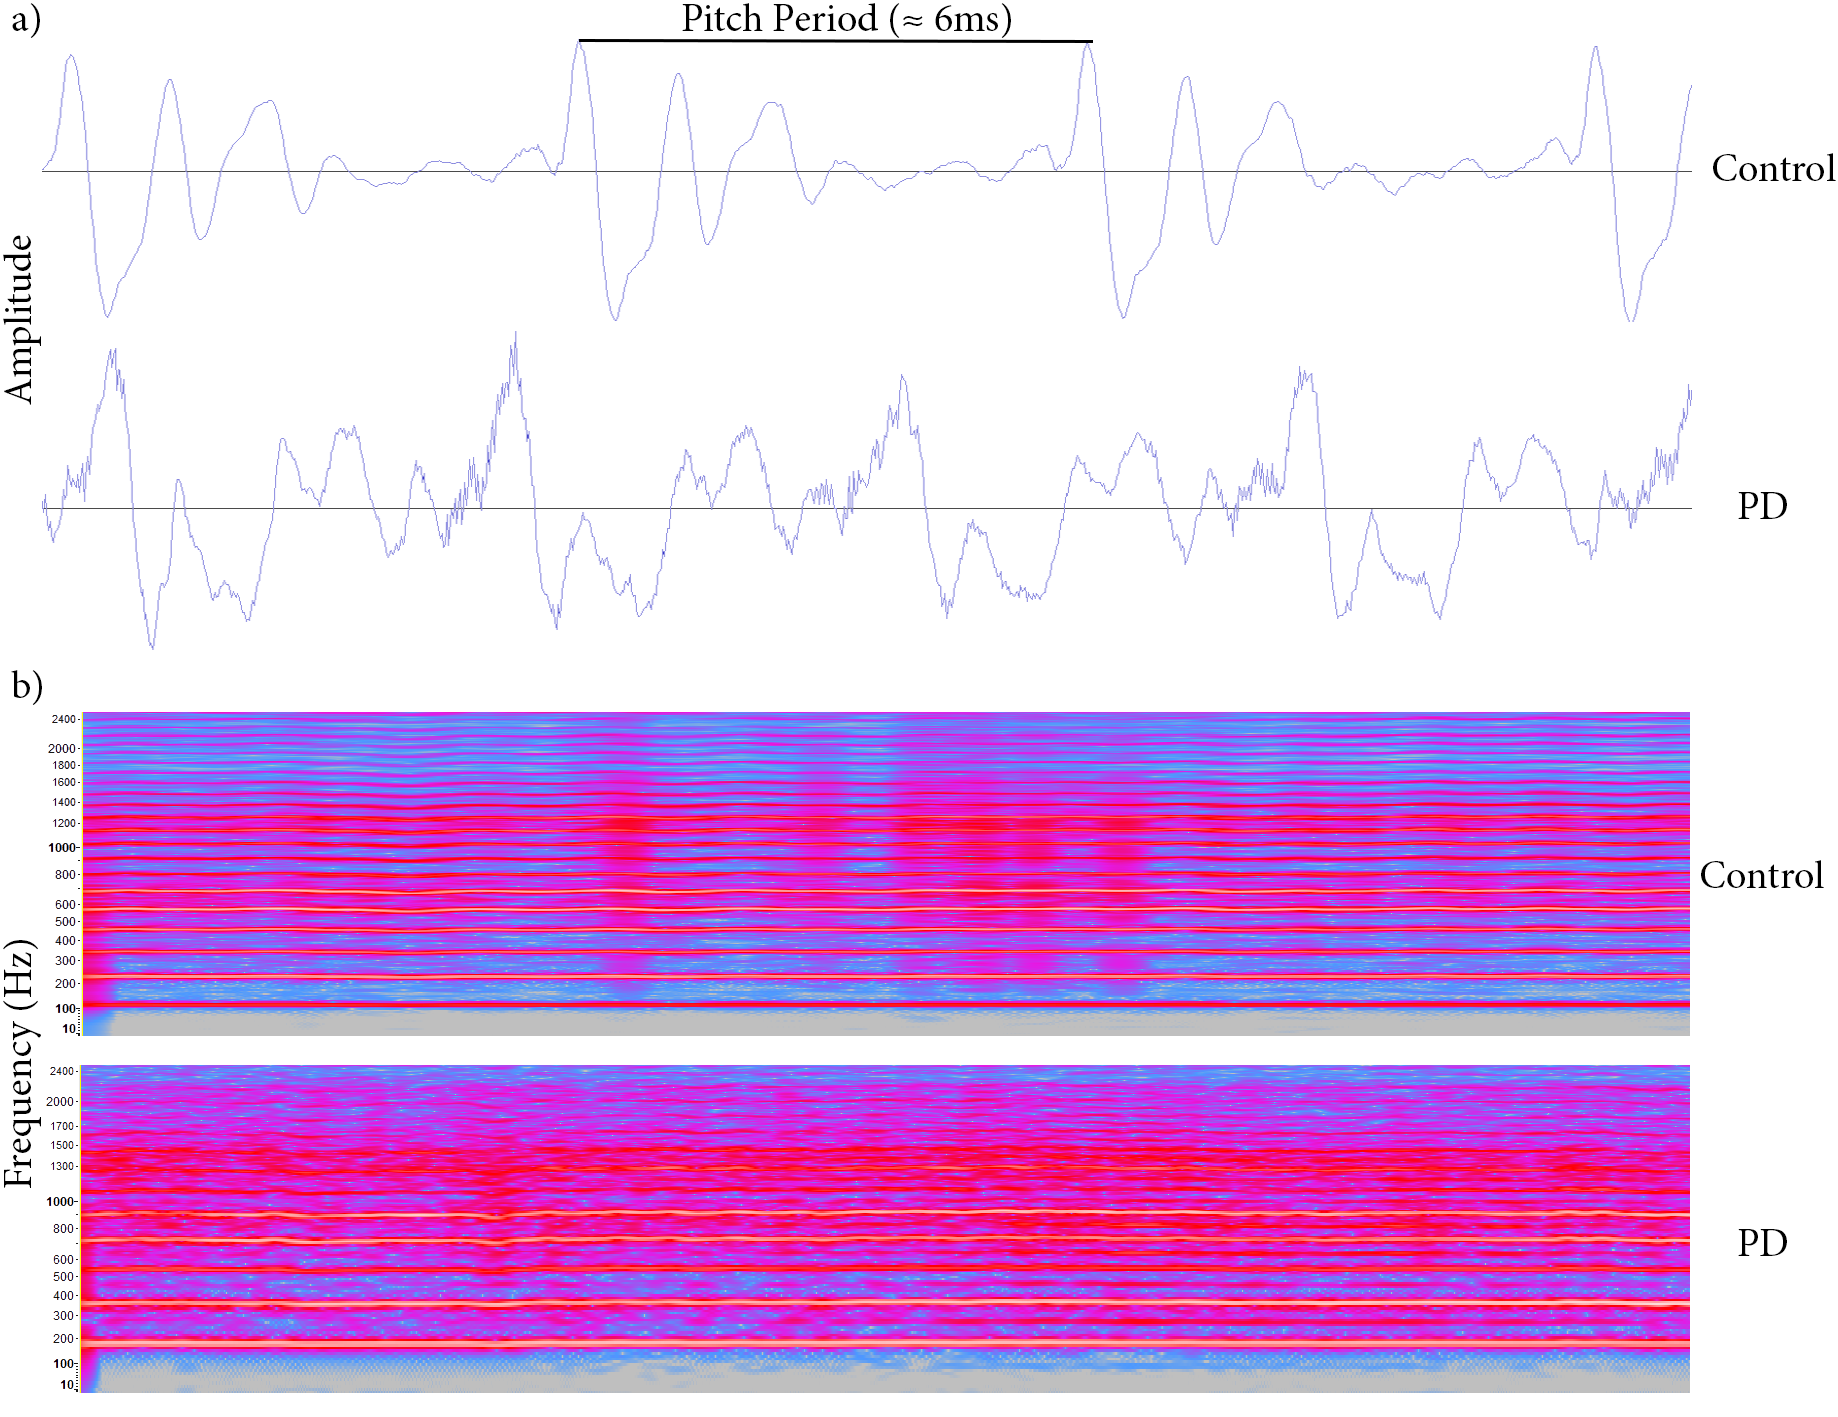
\includegraphics[width=1.2\linewidth]{timespectrogram.png}}
	\caption{A visualisation of prominent dypshonia in /aa/ phonation on the time (a) and short time spectral domain (b, Mel-scale~\cite{mfscale}). Cases are generally not as extreme and the natural variation in voice makes differentiation a difficult task.}
	\label{spectrogram}
\end{figure}



%Features developed specifically for dysphonia are based on the non-linear model of speech production~\cite{splittledysphonia2009, splittlenonlinear2007}. 

%These features generally quantify the variation in each glottal cycle, relying on detection of the fundamental frequency ($f_0$). It should be noted that determining the $f_0$ from sustained vowel phonation is an inexact science~\cite{f0estimation}.


Tsanas~\cite{spoverview} extends GNE to develop the \textit{Vocal Fold Excitation Ratio} (\emph{VFER}). VFER is another quantification of the `breathiness' effect in dysphonic speech from turbulent airflow. Tsanas also introduces the Glottal Quotient (\emph{GQ}), which measures the standard deviation of the duration when the glottis is opened versus closed. Both VFER and GQ are built upon concepts of the DYPSA~\cite{dypsa} fundamental frequency estimation algorithm. 

Mel-Frequency Cepstral Coefficients (\emph{MFCC}) have long been used for speech recognition~\cite{mfcc}, and have also shown promise in detecting dysphonia~\cite{mfccml}. They are the most common and often the only feature used in speech recognition systems, but they lack interpretability and are very sensitive to noise~\cite{mfccrobust}. There are also a variety of feature sets used in general speech classification, such as the 6,368 feature ComParE set~\cite{is2013}. Although these features may not be designed specifically for dysphonia, they are effective in fields such as speaker trait classification and may be useful in providing contextual information for complex machine learning models. The incidence of PD varies based on age, gender and race~\cite{ageracial,racial}, and it is likely that dysphonia presents itself differently depending on speaker traits. We refer to Eyben~\cite{ostextbook} for a comprehensive description of these features as well as a summary of feature sets used in speech classification.


\label{dfadescription}
Methods used in non-linear dynamical systems\footnote{Dynamical systems theory is used to describe the behaviour of deterministic systems which appear to exhibit unpredictable behaviour based on a number of initial conditions. This will be explored further in \textit{\hyperref[eegsigproc]{Section}} \ref{eegsigproc}} have also been effective in dysphonia quantification~\cite{splittlenonlinear2007}. \textit{Detrended Fluctuation Analysis} (\emph{DFA}) was originally introduced as a measure of the autocorrelation\footnote{\emph{Autocorrelation} describes the similarity of a signal to itself when offset by a given interval.} of a signal~\cite{dfa}. Little~et~al.~\cite{splittlenonlinear2007} shows this correlates with the amount of turbulent airflow in speakers with dysphonia. Little~et~al. also proposes Recurrence Period Density Entropy (\emph{RPDE}), which characterises the periodicity of a signal. These measures are expected to be lower for speakers with dysphonia due to the noise introduced by turbulent airflow. Little~et~al.~\cite{splittledysphonia2009} builds upon RPDE to develop Pitch Period Entropy (\emph{PPE}) which is a better measure of the impaired control of pitch experienced by PD patients.


\subsection{Movement}\label{movementfeatures}
Despite a similar amount of literature existing in movement and voice feature engineering, signal processing in the voice domain is more developed. Feature engineering for movement data diverges into a number of subfields, each developing different measurements for different sensors to quantify the extent of a movement disorder. %Features are crafted specifically for dyskinesia\footnote{\emph{Dyskinesia} describes the presence of involuntary, often `jerky' movements.} and akinesia\footnote{\emph{Akinesia} is the impairment of voluntary movement.} quantification. The signal processing techniques used in movement disorder quantification are basic compared to methods in voice.

People with PD exhibit increased tremor, particularly in the 3.5-7Hz range~\cite{duval2004detection}, as well as distinct patterns of postural sway. Mediolateral (left-right) sway is generally a better indicator of PD than Anteroposterior (forwards-backwards) sway~\cite{posturalswaylongitudinal}. A Fourier transform can quantify the amount of tremor in IMU sensor data. Postural sway is best measured when the subject attempts to stand as still as possible. Both IMUs and force plates can quantify this --- IMUs have the advantage of being cheaper and more accessible; however, have lower resolution and may not be spatially accurate~\cite{palmerini2011tremor}.  Medication such as Levodopa is known to significantly increase the amount of postural sway~\cite{posturalswaylongitudinal}.



%, and recurrence can be quantified with techniques such as RPDE (\textit{\hyperref[dfadescription]{Section}} \ref{dfadescription}).


 
Abnormal gait is another major indicator of Parkinson's disease. Gait related symptoms are mostly presented in the forms of Bradykinesia and Akinesia. \emph{Bradykinesia} describes the slowness of movement, with individuals with PD generally showing a decreased cadence (steps per minute) and stride length~\cite{esser2011assessment}. \emph{Akinesia} describes the involuntary loss of movement, and often presents itself in the form of `freezing of gait,' where a patient experiences a sensation like their feet being glued to the ground~\cite{giladi1992motor}. Individuals with PD also exhibit interesting heel-to-toe characteristics, where their foot lands flat on the ground (as opposed to the heel striking the ground first, as in regular gait)~\cite{heeltotoe, roiz2010gait}.

Gait can be quantified using IMUs, force walkways and motion capture. IMUs are undoubtedly the cheapest and most available option; however, gait characteristics can only be estimated. IMUs attached to the foot shank allow relatively precise estimation of step length and cadence \cite{barth2011biometric, sijobert2015implementation}, whereas handheld or in-pocket gait estimation is a more challenging task~\cite{renaudin2012step,diaz2014step}. IMUs and other sensors embedded in the shoe can quantify heel-to-toe characteristics. Force Walkways and motion capture are more precise, but costly alternatives for measuring gait.

%Although expensive and difficult to set up, motion capture presents the possibility of completely quantifying all movement-related components. However, feature engineering has not evolved to take advantage of the additional information and a significant amount of training data would likely be required to realise its full potential. Das~et~al.~\cite{das2011quantitative} uses motion capture on 4 PD and 2 control subjects, yet does not explore advanced spatial features beyond what is provided by multiple accelerometers. Pose recognition in video is also an rapidly developing field which proposes similar capabilities to motion capture at a fraction of the cost. Current models are promising, however are not precise enough to be used in combination with akinesia detection~\cite{toyer2017human}.

\subsubsection{Smartphones}
Smartphones are one of the fastest adopted technologies in history, becoming increasingly prominent in developing countries. As they possess a number of sensors such as IMUs, microphones and cameras, they are a promising tool in \textit{telemedicine} --- the remote diagnosis or monitoring of PD. The universal nature of smartphones allows for large PD datasets, with the 8,000 participant mPower~\cite{mpower} dataset used in this paper crowdsourced from smartphone users.

Smartphone studies use features presented in voice and accelerometer research, along with additional tests such as memory or tapping tasks~\cite{tapping}. However, the resolution and accuracy of smartphone sensors greatly varies and introduces significant noise to the data. The influence of smartphone models on results has yet to be investigated, and it is unknown whether generalizing between phones is possible. Smartphone step and motion mode recognition\footnote{\emph{Motion mode recognition} involves classifying whether the user has their phone in their pocket, hand, bag  }~\cite{motionmoderecognition, li2010multimodal} is a similar research area; however, techniques are less applicable as measures are often more coarse.


Little~et~al.~\cite{splittledysphonia2009} provides evidence that a high quality microphone is not required to classify dysphonia, obtaining good results with phone-call recordings. Brunato~et~al.~\cite{smartphonemjfoxlion}, Boussios~et~al.~\cite{smartphonemjfoxB} and Arora~et~al.~\cite{arora2014high} also manage to obtain good results with simple smartphone IMU-based features. However, all of these models have been tested on small datasets, which are prone to overfitting on cross validation~\cite{overfittingcv} from bias and uninformative predictors~\cite{freedmanparadox}. 


Zhan~et~al.~~\cite{zhan2016high} conducted a smartphone feasibility study on the largest dataset to date --- 121 PD and 105 controls. Participants were recruited into the study and asked to peform tasks such as walking, saying /aa/ and alternated tapping~\cite{tapping}. However, Zhan~et~al. obtained 71 per cent accuracy --- especially poor considering that the mean (standard deviation) age of PD subjects was 57.6 (9.4) and control 45.5 (15.5). A similar result may be obtained by a model classifying with age alone. This result is in direct contradiction with previous works such as Arora~et~al.~\cite{arora2014high} which reported 98 per cent accuracy on very similar accelerometer features. It is clear that reported results must be taken with a grain of salt. %Zhan~et~al. also uses very basic features to quantify speech, neglecting the state of the art speech signal processing features used in other works~\cite{ostextbook, spoverview}. 

%A possible cause is that Zhan~et~al. does not control the android smartphone used, hence the sensor data collected varies significantly between devices. 

Neto~et~al.~\cite{mpowerneto2017analysis} is the first study based on the 6,000 participant mPower dataset~\cite{mpower}. Neto~et~al. focused on the data analysis aspect, investigating the impact of medication and the ``time of the day'' effect on activity performance. The features used in this analysis are not described --- the author list and citations suggest that accelerometer features used were an extension of Arora~et~al.~\cite{arora2014high}. 

Neto proposed a method of ``collapsing'' multiple recordings for a participant into one by taking the median value of each feature over all the recordings. This improves model performance, but may not be entirely valid. In mPower, participants with PD often perform more recordings than other participants, who are likely less serious about the study. When taking the median of feature values, unrealistic combinations of values may arise as they may be from different recordings. The model may be learning to associate PD with these strange combinations of `median-like' values.

\subsection{EEG}
\label{eegsigproc}
Electroencephalogram (EEG) signal processing presents an interesting challenge as the characteristics of an EEG signal are less well understood compared to speech and motion. There are specific features for diagnosis PD or Alzheimer's disease\footnote{Alzheimer's disease is a similar neurodegenerative disease. It is characterised by a loss of neurons in the cerebral cortex whereas PD targets dopaminergic neurons.}; however, this section will focus on the techniques applicable to speech and movement data.

Non-linear dynamical systems theory inspires many EEG signal processing techniques, as EEG signals are believed to be generated by non-linear coupling interactions between neuronal populations~\cite{eegalzheimers}. Patients suffering from neurodegenerative disorders often exhibit decreased complexity in EEG patterns, believed to be caused by the a decrease in  non-linear cell dynamics~\cite{jelles1999decrease}. Features developed with EEG signal processing aim to characterise the dynamic structure of this system. As these features are not related to human senses, they may be promising when applied to the task of measuring the presence of voice or movement symptoms undetectable by a neurologist. 

\begin{highlight}
The nature of features used in EEG make them promising for the task of detecting the presence of symptoms undetectable by a neurologist.
\end{highlight}


\emph{Chaos theory} is a field analysing systems which are sensitive to initial conditions. One can imagine the generation of a speech signal as a system, where parameters involve the state of components in the vocal tract. Given no change in parameters such as vocal fold tension, regular /aa/ phonation can be modelled with much fewer dimensions in \textit{phase}\footnote{The \emph{phase} space represents all possible states of a dynamic system.} space~\cite{denoisingchaos, vocalchoas}. A recurrence plot is commonly used to understand chaotic systems and is depicted in \textit{\hyperref[recurplot]{Figure}} \ref{recurplot}.


\begin{figure}[!htb]
	\centerline{
		\begin{subfigure}[]{0.4\textwidth}
			\caption{Healthy Speech}
			\centering
			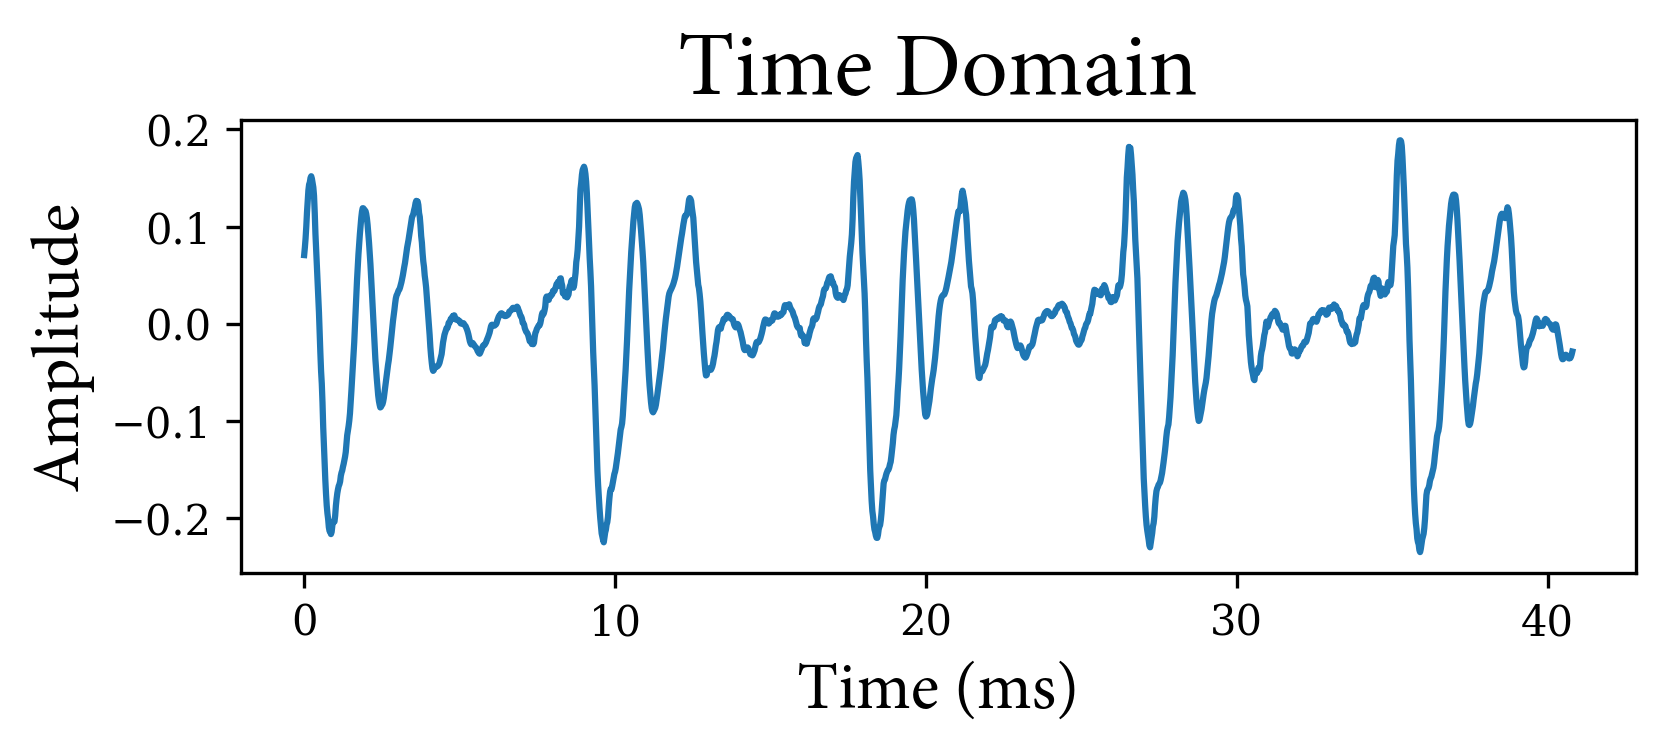
\includegraphics[width=0.96\linewidth]{healthy_time.png}
		\end{subfigure}%
		\hspace{3em}
		\begin{subfigure}[]{0.4\textwidth}
			\caption{Dysphonic Speech}
			\centering
			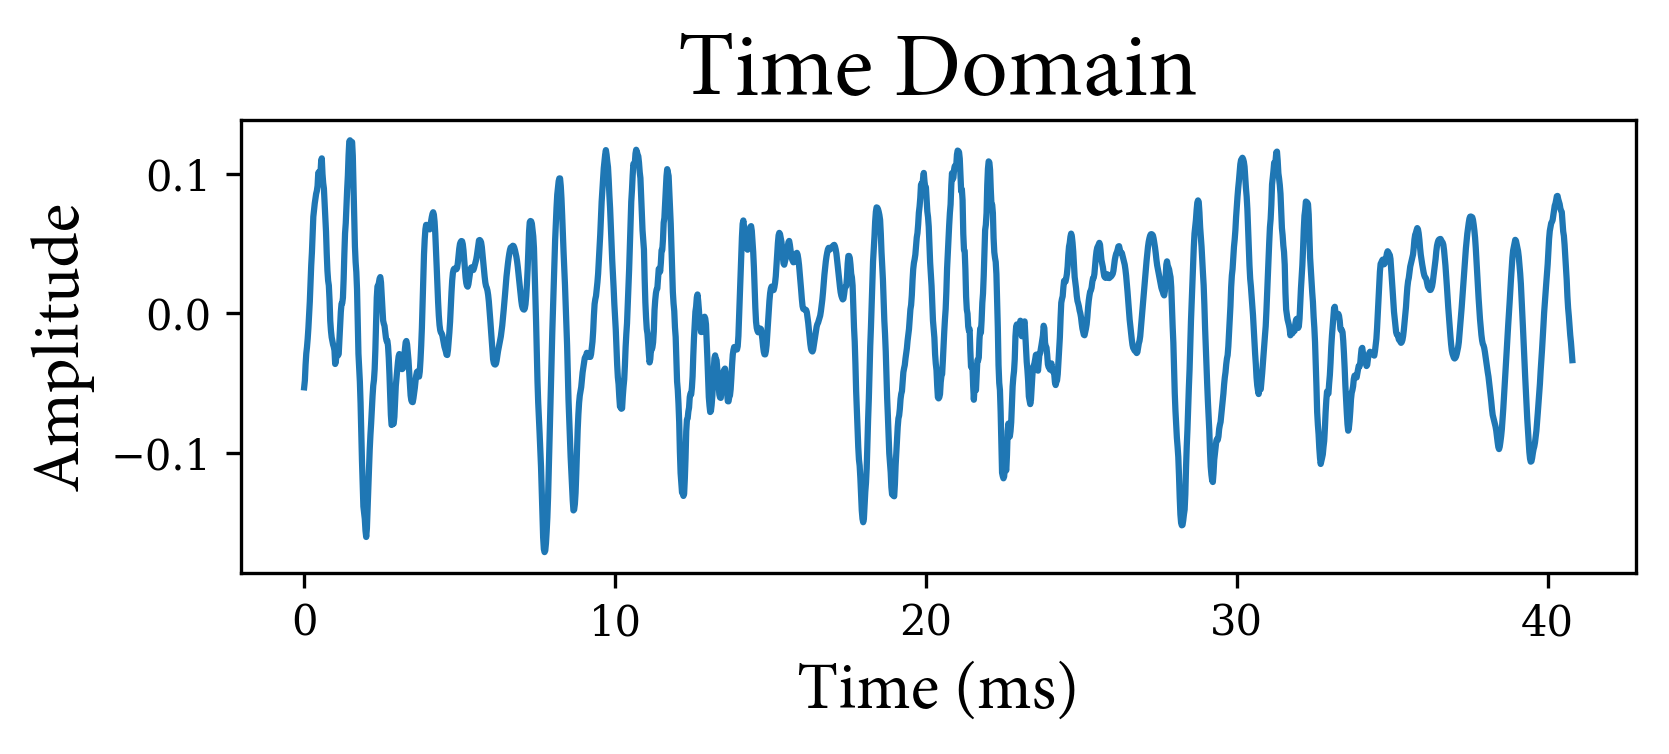
\includegraphics[width=0.96\linewidth]{pd_time.png}
		\end{subfigure}
	}
	
	\centerline{
		\begin{subfigure}[]{0.4\textwidth}
			\centering
			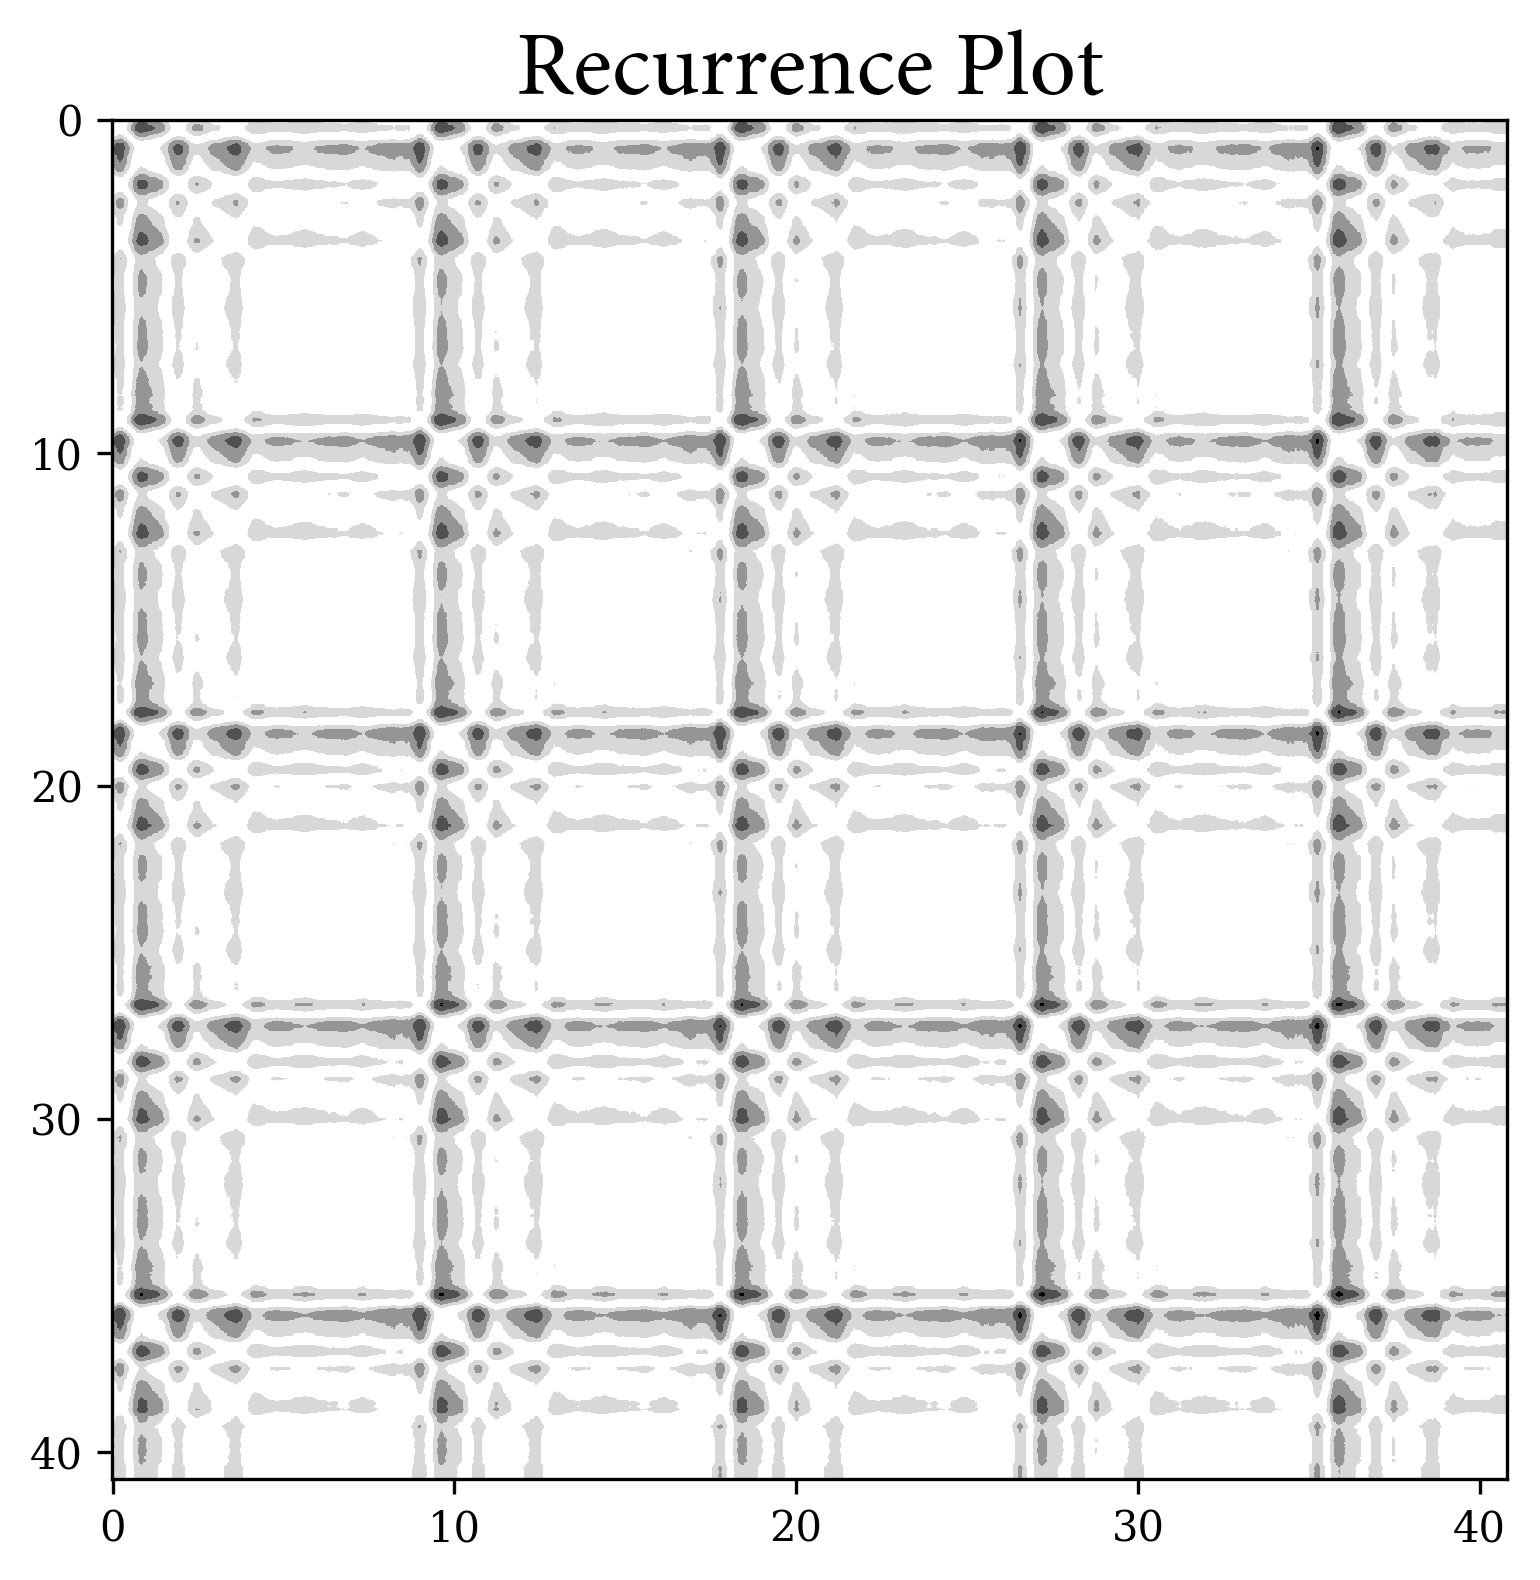
\includegraphics[width=0.96\linewidth]{healthy_rplot.png}
		\end{subfigure}%
		\hspace{3em}
		\begin{subfigure}[]{0.4\textwidth}
			\centering
			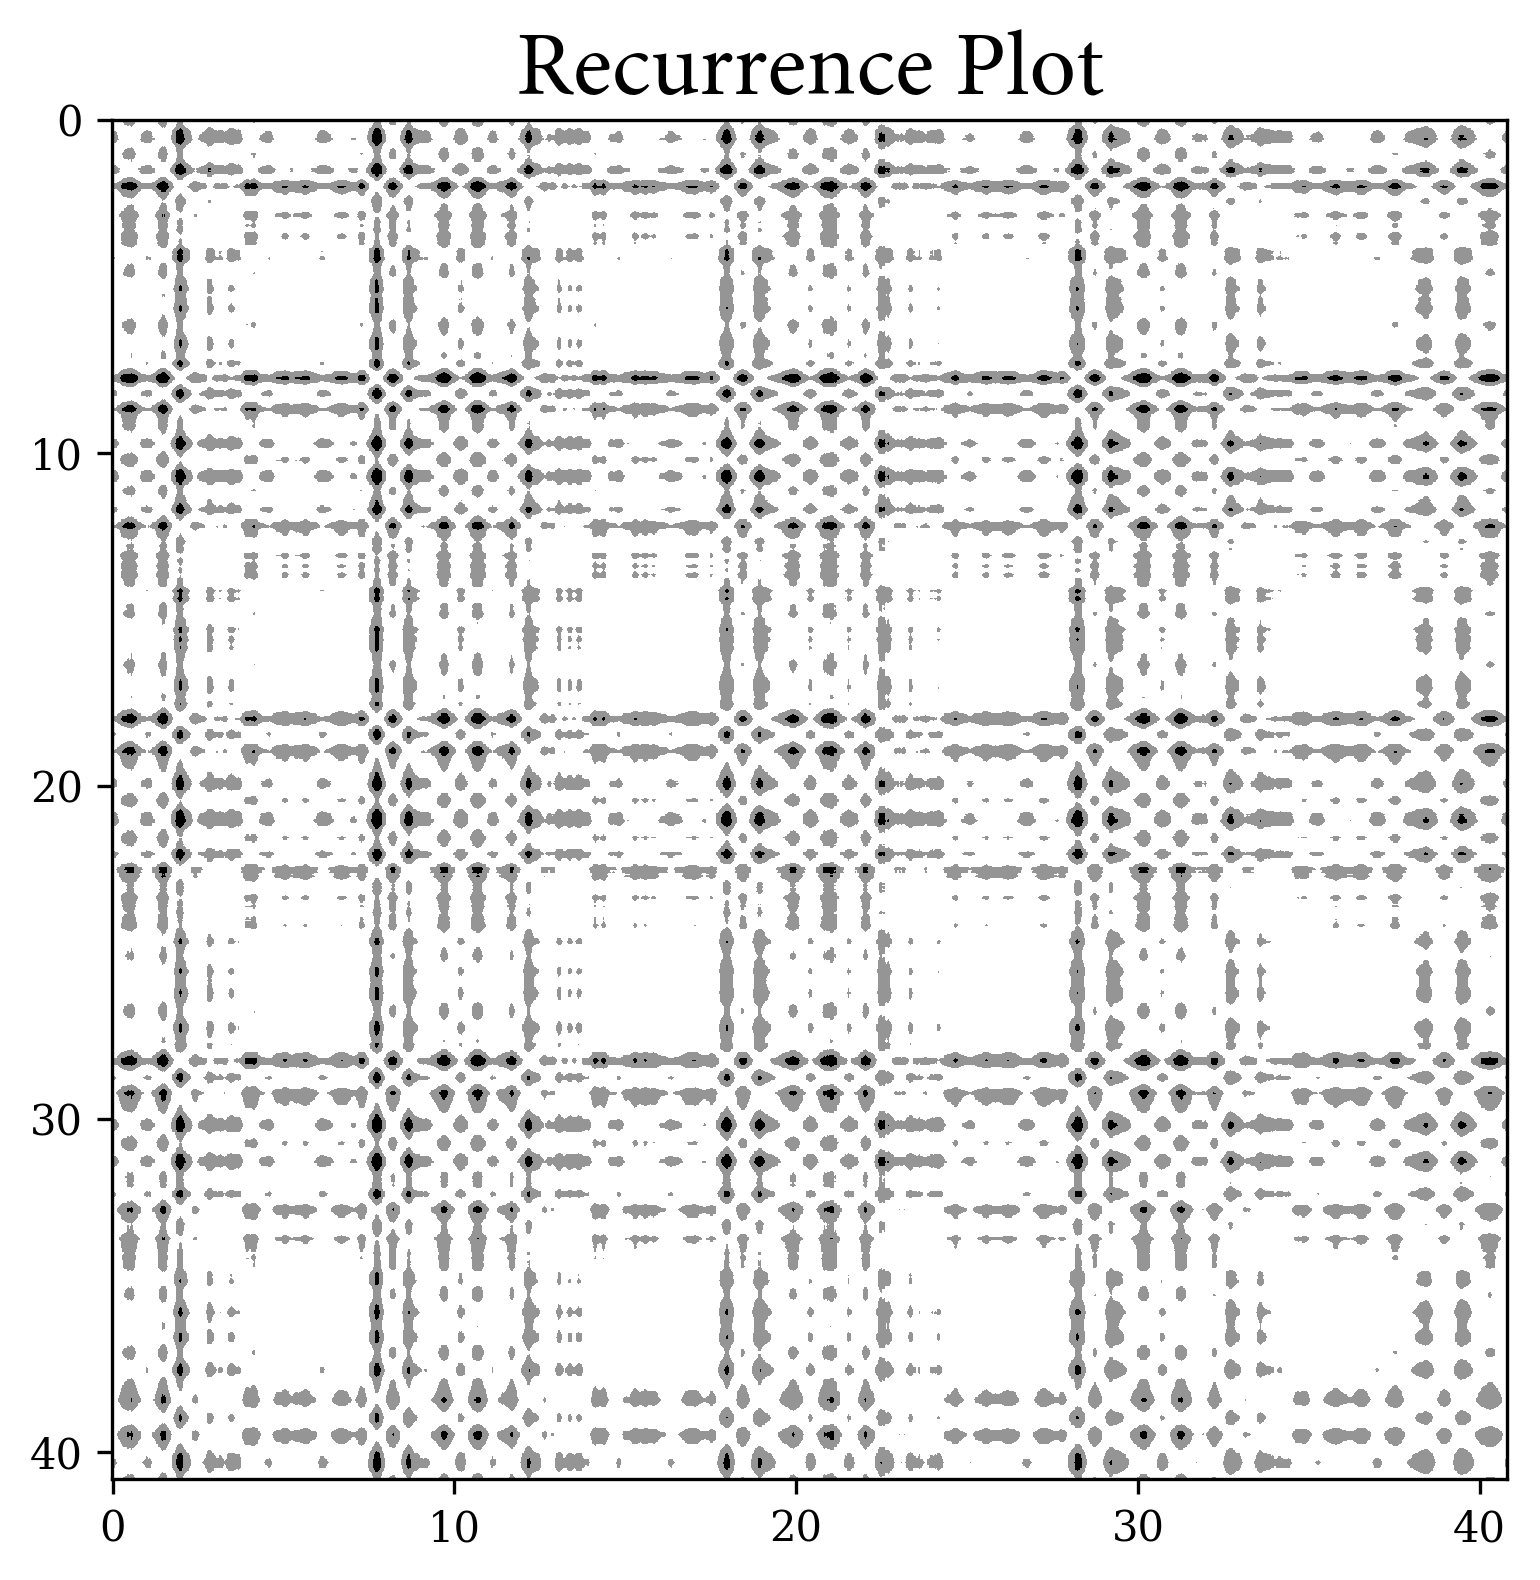
\includegraphics[width=0.96\linewidth]{pd_rplot.png}
		\end{subfigure}
	}
	
	\centerline{
		\begin{subfigure}[]{0.4\textwidth}
			\centering
			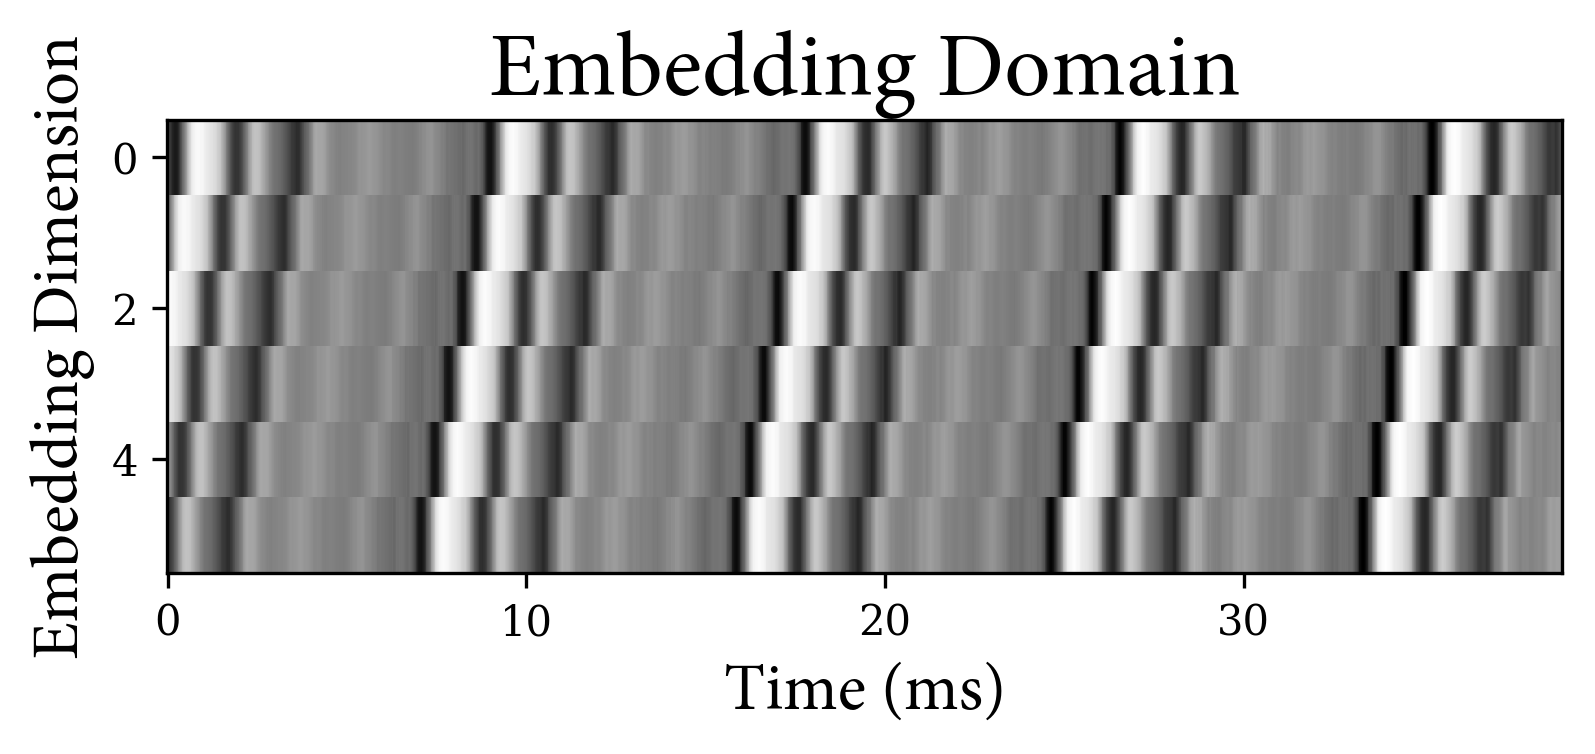
\includegraphics[width=0.96\linewidth]{healthy_embdim.png}
		\end{subfigure}%
		\hspace{3em}
		\begin{subfigure}[]{0.4\textwidth}
			\centering
			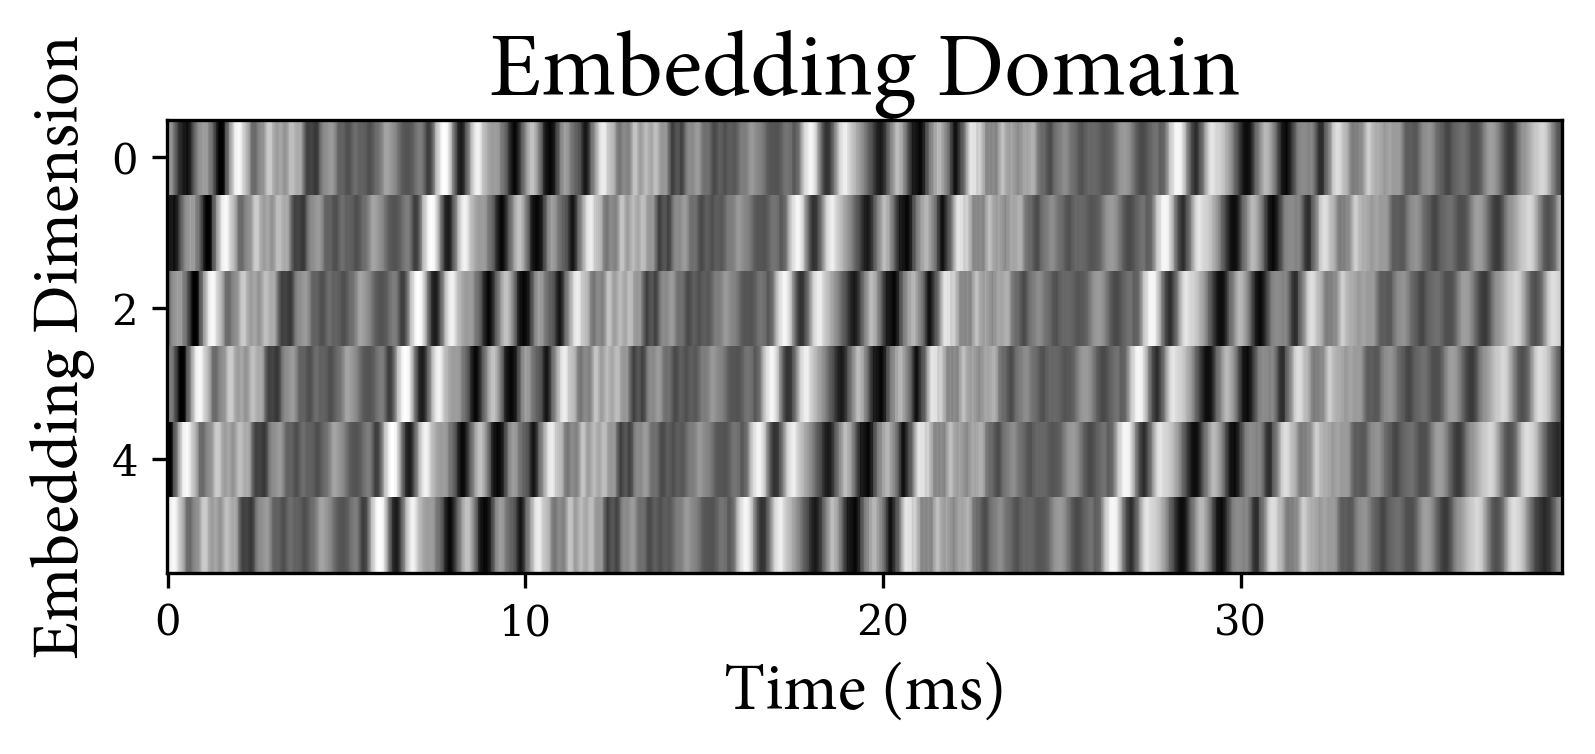
\includegraphics[width=0.96\linewidth]{pd_embed.png}
		\end{subfigure}
	}
	\caption{A visualisation of speech on various domains. The recurrence plot~\cite{recurrenceplots} was developed to visualise the periodicity of a signal, highlighting where the system approximately reaches the same state. The time-lagged embedding domain is used by Rosenstein~et~al~\cite{rosenstein1993practicallyapunov} to calculate non-linear measures such as the largest Lyapunov exponent and in measures such as Fisher Information or SVD Entropy.}
	\label{recurplot}
\end{figure}


The \emph{Lyapunov Exponents} quantify the divergence of two systems with infinitesimally similar initial parameters. The \textit{Largest Lyapunov Exponent} (\emph{$\lambda^*$}) characterises the chaos in a system and is commonly estimated with Rosenstein's algorithm~\cite{rosenstein1993practicallyapunov} which reconstructs the system's dynamics using a time delay technique. Its inverse, $\frac{1}{\lambda^*}$ is the Lyapunov time, which defines how long the behaviour of a system can be predicted. The $\lambda^*$ has long been used in the EEG analysis of sleep and as a feature for machine learning~\cite{eeglyapunov1, eeglyapunov2}. The $\lambda^*$ have also been applied in the analysis of speech~\cite{banbrook1999speechlyapunov,kokkinos2005nonlinearlyapunov}, gait and balance ~\cite{dingwell2000nonlinearlyapunov, howcroft2014analysisgaitlyapunov, liu2015analysislyapunov}.



%\footnote{Accurate estimations of additional Lyapunov exponents generally require known equations describing the system~\cite{lyapunovall}. Eckmann's algorithm~\cite{eckmann1986liapunov} can roughly estimate these exponents.}

%\begin{figure}[!htb]
	%\label{LLE}
	%\centering\centerline{
\includegraphics[width=1.2\linewidth]{attractor.png}}
	%\caption{$\lambda^*$ describes the trajectory of a system's %\textit{attractor}. First three dimensions of the reconstructed attractors %from /aa/ and /s/ phonation depicted. Image from %Kokkinos~et~al.~\cite{kokkinos2005nonlinearlyapunov} }
%\end{figure}



%The term as coined by Mandelbrot in 1967~\cite{mandelbrot1967long}

The \emph{fractal dimension} is another measure commonly used in the analysis of EEG and other dynamical systems along with the LLE. It represents the ratio of the log change in detail to log change in scale of a signal\footnote{The coastline paradox is the observation that as you measure a coastline with increasingly smaller measuring sticks, the measured coastline length will increase. The \emph{fractal dimension} would measure the ratio of change in length as of the `stick' used to measure the coastline is made shorter.}~\cite{mandelbrot1967long}. A higher value correlates to a more complex signal, and the fractal dimension of an EEG signal with open vs. closed eyes and normal vs. epileptic states are observably smaller~\cite{eegfractal, seizuredimensions}. The fractal properties exhibited in neuronal control are reflected in heartbeat and gait~\cite{fractalgait} with force plate data from elderly and Parkinsonian subjects showing a significant increase in fractal dimension compared to healthy young subjects~\cite{hfdcop, fractalpd, fractalbalance}. Esteller et~al.~\cite{fractaldimensions} compares algorithms estimating the fractal dimension of signals.


\emph{Fisher Information} is a measure relating to the uncertainty of measuring a variable (signal) about the unknown parameters modelling its distribution~\cite{fisherentropy}. It is applicable in quantifying non-linear dynamics~\cite{fisherinfo} and has been applied in the analysis of EEG~\cite{fisherinfo2}. General entropy will not differentiate two sequences where the frequency of each variable is the same; however, the sequences 0,0,0,0,1,1,1,1 and 0,1,0,0,1,1,0,1 are clearly generated by different stochastic processes. \emph{Approximate} and \emph{sample entropy} are similar measures to entropy; however, they quantify this unpredictability in a signal~\cite{apsampentropy, apentropy}. The multi-scale sample entropy~\cite{multiscaleentropy} is especially powerful tool in the analysis of biological signals~\cite{samplegaitmulti, sampleheart}. Although approximate and sample entropy are prominently used in EEG signal processing, they are rarely applied to voice and movement analysis. 

Although signals may appear to have high information content on the time domain, they may be easier to represent on others. For example, the JPEG image compression format~\cite{jpeg} primarily relies on the inability of human vision to perceive high frequency information. Images are compressed by taking a Fourier transform and reducing the amount of high frequency information. \emph{Spectral entropy} measures the information content of the signal in its frequency domain representation. The singular value decomposition (SVD) factorises a matrix $M$ into $U\Sigma V$ where $U$ and $V$ are orthogonal matrices and $\Sigma$ is a diagonal matrix of \textit{singular values}.  \emph{SVD entropy}~\cite{svdentropy} measures the entropy of the singular values obtained when the signal is embedded with Rosenstein's~\cite{rosenstein1993practicallyapunov} technique. 

Like DFA, the \emph{Hurst} exponent characterises the autocorrelation of a signal~\cite{hurst}. DFA is a generalisation of the Hurst exponent for non-stationary processes\footnote{Non-stationary systems are those with properties which evolve over time. A grid-like, repetitive recurrence plot (\textit{\hyperref[recurplot]{Figure} \ref{recurplot}} is indicative of a stationary system, whereas curved patterns are signs of a non-stationary, chaotic system~\cite{facchini2005recurrence}}; however, DFA has been criticised for being biased towards underestimation in short signal recordings, and its ability to address non-stationary signals questioned~\cite{revistDFA}. For self-similar signals, the Hurst exponent relates directly to the fractal dimension. In general the measures are independent, with the Hurst exponent characterising the global rather than local properties of a signal~\cite{hurstfractal}. A Hurst exponent less than 0.5 characterises the signal `switching' between high and low values, 0.5 characterises random walk like behaviour, and values greater than 0.5 imply positive autocorrelation. Like fractal dimension, the Hurst exponent is a valuable tool in the analysis of gait and balance~\cite{duarte2000fractal}. 

\vspace{22em}
\subsection{Summary of Features}
\textit{\hyperref[genfeatsum]{Tables}} \ref{genfeatsum} to \ref{eegfeatsum} summarise all of the features used in the construction of models presented in this thesis. The libraries and parameters used to implement them are described in \textit{\hyperref[implementation]{Section}} \ref{implementation}. Features are organised by field of introduction or by their most applicable field. All relevant general and EEG features are calculated for both the audio and accelerometer models used in this thesis. Additionally, RPDE and DFA are used as a feature in accelerometer based models.

\label{featuresummary}
% \centering
\bgroup
\def\arraystretch{1.3}%
\begin{longtable}{r p{114mm}}
\caption{Features and techniques which are applicable to any signal processing problem.}
\label{genfeatsum}\\
\multicolumn{2}{c}{\specialcellbold{General Signal Processing}} \\
\midrule 
\vspace{-0.2em} Feature & \vspace{-0.2em} Description \\
\midrule
Moments & Statistical features --- mean, variation, skewness, kurtosis, etc.\\
Crossing Rate & Rate the signal oscillates around a value --- usually zero or the mean.\\
\specialcellright{Information\\ \hspace{1em}Theoretic} & Entropy, mutual information, cross-correlation and related measures based on the information content of signal. \\
Spectral Flux & Rate at which the power spectrum changes\\
Fourier & Transforms the signal from time domain to frequency/spectral domain. Quantifies the \textit{power} of a signal at a given frequency.\\
Wavelet & A variation of the Fourier transform with a different bases, allowing it to quantify both time and frequency\\
\specialcellright{\hspace{3em}Energy\\Operators~\cite{tkeo}}& Quantifies the instantaneous amplitude and frequency of a signal. Common operators are Teager-Kaiser (TKEO) and Squared (SEO) \\
\midrule 
\end{longtable}

\begin{longtable}{r p{114mm}}
	\caption{Dysphonia signal processing generally quantifies the variation in each glottal cycle during speech production}\\
\multicolumn{2}{c}{\specialcellbold{Voice -- Dysphonia}} \\
\midrule
 \specialcellright{Power\\Cepstrum} & From the inverse Fourier transform. Commonly taken in the Mel-log scale~\cite{mfscale}, resulting in the MFCC~\cite{mfcc}. Minimal interpretability, though it is the primary feature used in speech recognition~\cite{mfccml}. \\
Pitch~\cite{f0estimation} & Although obtainable with a Fourier transform, pitch often refers to estimating the exact duration of each glottal cycle.\\
Loudness & The volume of a sound in relation to human hearing. Only meaningful if recording setup is strictly controlled.\\
Formants & The resonance frequencies of an audio sample.\\
HNR~\cite{HNRintro,HNRperiodic} & Measures the ratio of noise in a voiced signal (signal to noise)\\
Jitter~\cite{jittertime} & Measures of the variation between the length of each glottal cycle. \\
Shimmer~\cite{shimmerjitter} & Measures of the variation of amplitude between each glottal cycle. \\
LPCC~\cite{lpcc} & Coefficients of an \textit{autoregressive} model which measures how well a signal can be modelled linearly by its previous values.\\
GNE~\cite{gne} & An extension of HNR by Michaelis et~al.~\cite{gne} to improve reliability in dysphonia quantification. \\
VFER~\cite{tsanas2012novel} & An further extension of HNR, building upon the theory of GNE.\\
EMD-ER~\cite{EMDER} & Another technique developed based on non-linear speech theory to quantify signal to noise\\
GQ~\cite{tsanas2012novel} & Measures standard deviation of duration the glottis is opened vs. closed.\\
DFA~\cite{splittlenonlinear2007, dfa} & Detrended Fluctuation Analysis. A generalisation of the Hurst exponent which measures the autocorrelation of a time series.\\
RPDE~\cite{splittlenonlinear2007} & Measures the periodicity of a signal, specifically designed with non-linear speech as the target.\\
PPE~\cite{splittledysphonia2009} & Measures the stability of pitch in sustained phonation.	\\
\specialcellright{\hspace{1.9em}Wavelet\\Measures~\cite{sptsanastelemonitor2010}} & A set of 180 measures for dysphonia based on wavelet transforms to the $f_0$ of speech introduced by Tsanas~et~al.~\cite{tsanas2011nonlinear}.\\
\specialcellright{GeMAPS~\cite{geneva}} & A minimal acoustic feature set of 58 or 87 (eGeMAPS) parameters that performs well in general speech classification~\cite{ostextbook}.\\
\specialcellright{\hspace{1.3em}Interspeech\\ComParE~\cite{compareis13featureset}} & An exhaustive 6,368 feature set for general speech classification~\cite{ostextbook}. Feature/dimensionality reduction generally improves performance unless data is plentiful.
%\\\specialcellright{Hammarberg\\ \hspace{0.2em} Index~\cite{hammarberg1980perceptual}} & The ratio of the strongest energy peak from 0-2kHz versus 2-5kHz. The \textit{Alpha Ratio} is similar, measuring the largest peak 50Hz-1kHz versus 1kHz-5kHz.\\
\\
\midrule
\end{longtable}


\begin{longtable}{r p{114mm}}
	\caption{There are few movement specific features, with most based on simple measures of postural sway or irregular gait.}\\
\multicolumn{2}{c}{\specialcellbold{Movement}} \\
\midrule
\specialcellright{\hspace{2.5em}Fourier\\\hspace{2.7em}Bands} & The power in bands such as 3.5hz-7hz compared to 7hz-12hz are the primary features used to detect Parkinsonian tremor.\\
Jerk~\cite{jerkfeature} & The change in acceleration. The jerk signal may be more effective when combined with certain signal processing methods.\\
\specialcellright{Sway\\Area} & This can be calculated na\"{i}vely by multiplying the range of sway in the A/P and M/L directions or by fitting a bounding ellipse in the principal component axis~\cite{pcasway}. As A/P and M/L directions are lost in accelerometer data, the bounding ellipse method is used.\\
\specialcellright{Cadence\\Measures} & The steps per minute, variation in time taken for each step, difference between left and right stride times.\\
\specialcellright{\hspace{1em}Stride\\Measures} & The length of each step and variation in step lengths. This was not measured as leg length is not available in the dataset used~\cite{diaz2014step}.
\\ 
\midrule
\end{longtable}

\vspace{2em}

\begin{longtable}{r p{114mm}}
	\caption{EEG signal processing is often based on non-linear systems theory. These features may be effective in detecting the presence of symptoms invisible to neurologists.}
	\label{eegfeatsum}\\
\multicolumn{2}{c}{\specialcellbold{EEG}} \\
\midrule
\specialcellright{\hspace{3.6em}Hjorth\\Parameters~\cite{hjorth}} & Three simple statistical measurements of a signal which have been used as features in EEG and IMU models~\cite{hjorthsmartphone}.\\
\specialcellright{\hspace{2em}Lyapunov\\Exponents~\cite{eckmann1986liapunov}} & Characterises the divergence of systems with close initial conditions. The largest exponent ($\lambda^*$)~\cite{dingwell2000nonlinearlyapunov} is generally the most informative. \\
\specialcellright{\hspace{3.3em}Fractal\\Dimension~\cite{mandelbrot1967long}} & A measure of how the detail in a signal changes with the scale at which it is measured. The Higuchi~\cite{hfd} and Petrosian~\cite{petrosian1995kolmogorov} fractal dimensions are used in this thesis.\\
\specialcellright{\hspace{3.2em}Hurst\\Exponent~\cite{hurst}} & Characterises self-similarity. DFA is a generalisation of the Hurst Exponent and is robust to non-stationary signals. The difference in measurements may be informative.\\
\specialcellright{Fisher Info~\cite{fisherinfo2}} & Quantifies the non-linear dynamics in the system generating a signal.\\
\specialcellright{\hspace{1.1em}Ap/Samp\\Entropy~\cite{apentropy}} & Approximate and sample entropy quantify the unpredictability of a signal. Multiscale entropy increases information content~\cite{multiscaleentropy}.\\
\specialcellright{Spectral\\Entropy} & Measures the regularity of the spectral (frequency) distribution. A high spectral entropy implies sharp differences in frequencies present in the signal.\\
\specialcellright{\hspace{2.9em}SVD\\Entropy~\cite{svdentropy}} & A measure of complexity. The entropy of the singular values of the signal after applying the time delay embedding method~\cite{rosenstein1993practicallyapunov}.
\\
\midrule
\end{longtable}


\egroup
% \end{table}
\section{Machine Learning}
\label{machinelearning}
\begin{highlight}
Fundamentally, the goal of machine learning is to use past data to make accurate predictions about new data. 
\end{highlight}

Machine Learning tasks can be classified as classification or regression, and supervised or unsupervised. Classification involves predicting the \textit{class} of a datapoint --- for instance, distinguishing PD from control --- whereas regression involves predicting a numerical value, such as the UPDRS motor scores. In supervised learning, the data is \textit{labelled} with the ground truth --- i.e., whether the subject has PD --- whereas an unsupervised model must find patterns in the data without any prior knowledge. This section will focus specifically on \emph{supervised binary classification} (two classes). 

Supervised binary classification can be viewed as `learning' a model which given a set of numerical input features, predicts a class 0 (control) or 1 (PD). This can be visualised as a function $f : \mathbb{R}^d \mapsto \{0,1\}$ where $d$ is the number of features used in the model. The edge where the $f$ transitions from zero to one is denoted the decision boundary (or `hyperplane') which partitions the data into the two classes. This is depicted in \textit{\hyperref[binaryclass]{Figure}} \ref{binaryclass}.


\begin{figure}[!htb]
\centering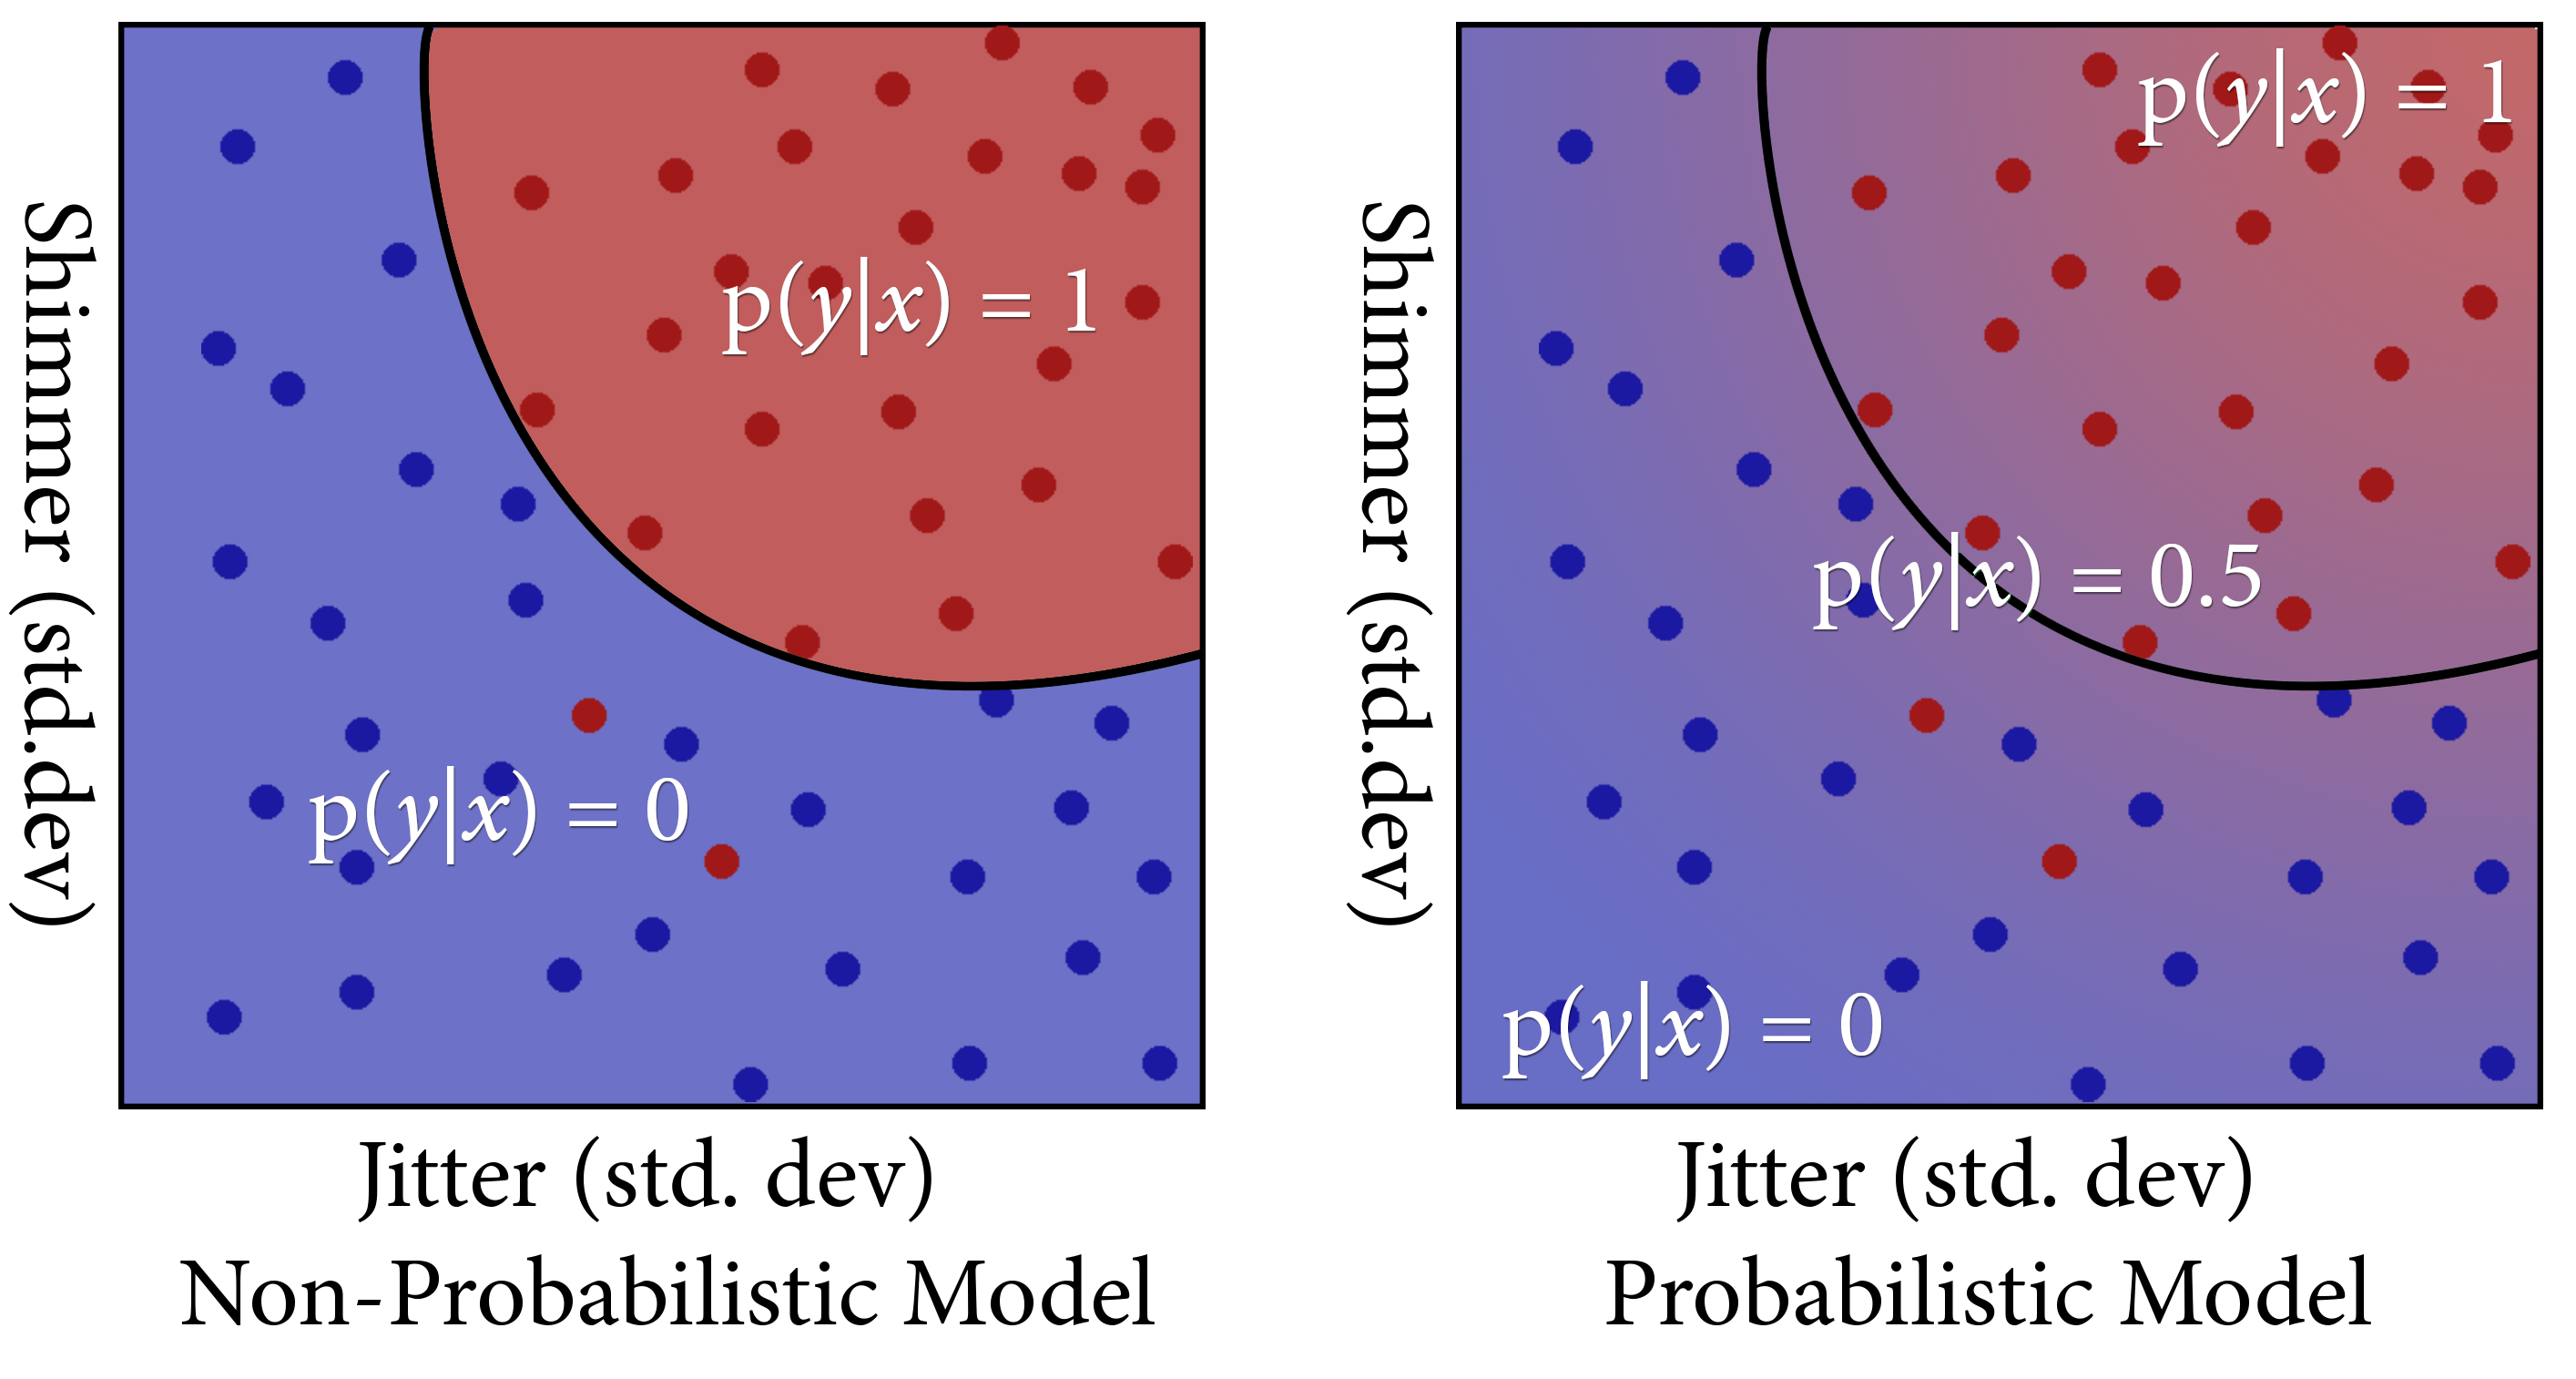
\includegraphics[width=0.7\linewidth]{binaryclassification2.png}
\caption{A visualisation of binary classification with two features. Data is rarely as `clean' as this artificial example.}
\label{binaryclass}
\end{figure}

Traditional machine learning models are built on solid statistical and mathematical foundations, and are well understood. However, these models have been developed on assumptions that are rarely satisfied by real-world data. Models such as deep neural networks have started to rise to popularity recently due to their modelling power; however, their behaviour is still poorly understood and they are difficult to analyse~\cite{visualisernn}.    

Models have strengths in different areas, and very rarely does a model strictly dominate another. The structure of the data informs the choice of model. For example, models like deep neural networks may perform well when data is plentiful, but in small datasets simple decision (\textit{\hyperref[traditionalmodels]{Section}} \ref{traditionalmodels}) trees may outperform neural networks (\textit{\hyperref[neuralnetworkintro]{Section}} \ref{neuralnetworkintro}).





\begin{highlight}
There is no `best' model --- the choice of model is informed by the data. 
\end{highlight}

The predictive error in any model can be decomposed as \emph{irreducible error}, \emph{bias} and \emph{variance}. Irreducible error occurs when the features used are too noisy\footnote{\emph{Noisy} in the context of machine learning of signal processing relates to the inherent variance of a measure. An inaccurate, low quality sensor can be considered `noisy'.} or unrelated to accurately predict the data. An optimal model cannot achieve performance beyond this irreducible error. Bias describes a model `fitting' the data poorly --- a model with high bias will have low accuracy. Variance describes how `unstable' a model is --- a model with high variance may score 100 per cent accuracy but generalise poorly to new data. A model with high variance is essentially predicting results by `memorisation.' Fitting a model with high variance is often known as \emph{overfitting}. The bias-variance tradeoff~\cite{biasvarnn} is a fundamental problem in machine learning, describing the difficulty in reducing bias without increasing variance and vice versa. Bias and variance are depicted in \textit{\hyperref[overfitex]{Figure}} \ref{overfitex}.

%Models often have one or more adjustable parameters to balance bias and variance. These parameters are tuned with intuition combined with some form of search~\cite{gridsearch, tpe}. 

\begin{figure}[!htb]
\centering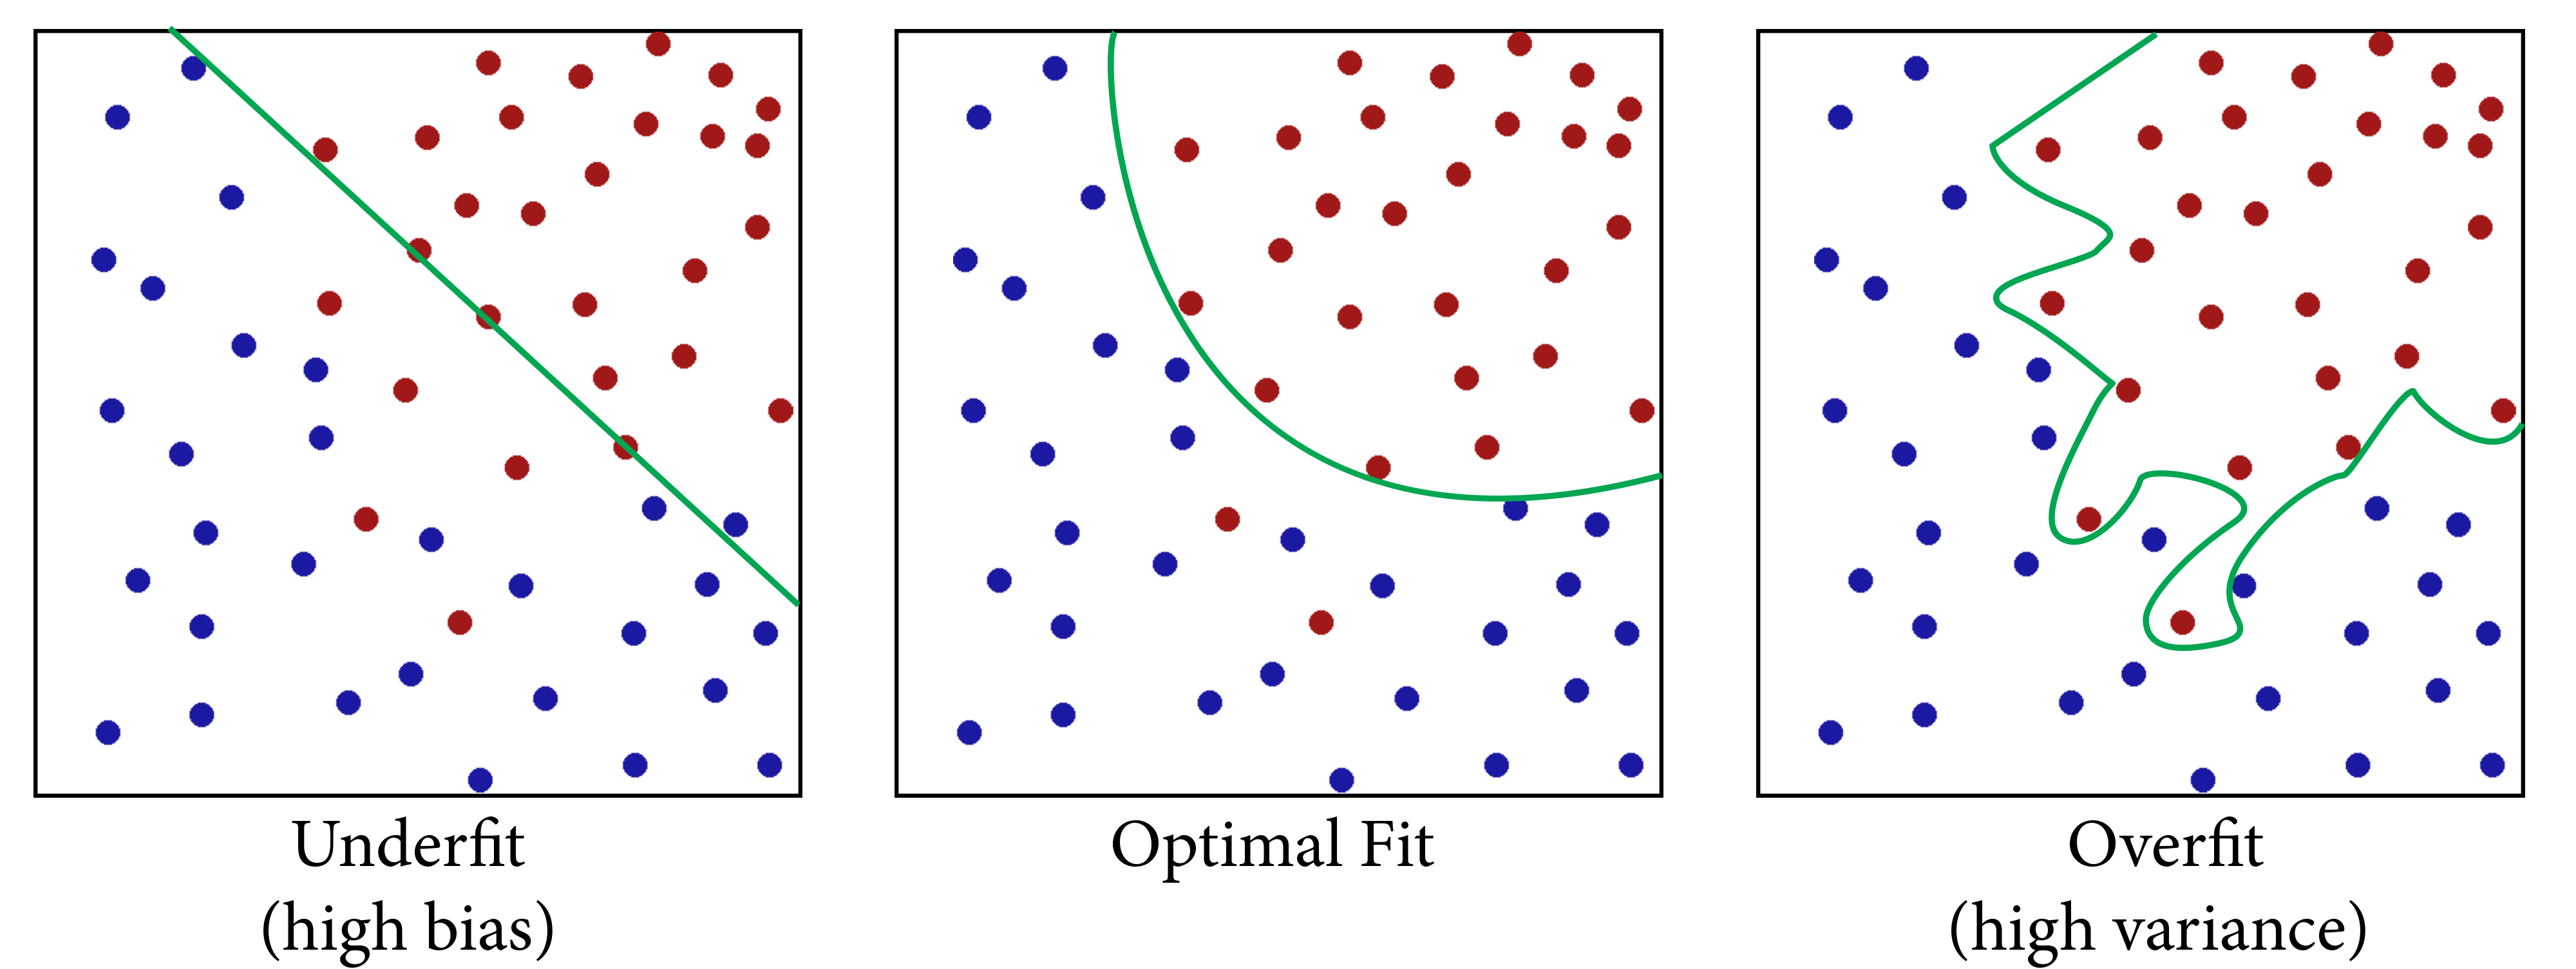
\includegraphics[width=0.95\linewidth]{overfit2.png}
\caption{Machine learning models and their parameters must be carefully chosen to ensure the optimal fit.}
\label{overfitex}
\vspace{-0.5em}
\end{figure}

Overfitting is a major issue in machine learning as data is limited and models are often too complex to analyse. Visualising and detecting overfitting may be simple when fitting a function in two dimensions, but it is significantly more difficult when the input has thousands of dimensions. Cross validation is the gold standard in machine learning when it comes to model evaluation and recognising overfitting; however, there are a number of caveats in its application. Cross validation, its caveats, and other techniques used for model evaluation will be discussed in detail in \textit{\hyperref[detectoverfit]{Section}} \ref{detectoverfit}. Like any statistics-based field, careful analysis of the results is required; unfortunately, this is often neglected in machine learning literature.


The following sections will cover three common models: random forest classifiers, support vector machines, and neural networks. The mathematical formulation of these models is abstracted in favour of intuition behind their behaviour. We refer to Bishop~et~al.~\cite{prml} for a formal description of these models.

 
\subsection{Traditional}
\label{traditionalmodels}
Traditional models are the approach favoured in current literature~\cite{review2013} due to the small dataset sizes. The two most popular models used are \emph{Random Forests} (of decision trees) and \textit{Support Vector Machines} (\emph{SVM}). Both of these are suitable for small datasets as they are relatively resistant to the curse of dimensionality\footnote{The \emph{curse of dimensionality} states that  exponentially more training data is often required for each additional feature to ensure a complete and reliable model.}~\cite{curseofdimensionality}. Both are also non-probabilistic classifiers\footnote{In general. Random forests and SVMs can provide pseudo-probabilistic output~\cite{svmprobabilistic}.}. There exists models which are inherently probabilistic such as Gaussian processes~\cite{rasmussen2006gaussian}, but these are often out-performed by decision-boundary based models in binary classification.

\emph{Random Forest}~\cite{randomforests} classifiers are derived on the concept of Bootstrap Aggregation  (\textit{bagging})~\cite{bagging} where the results of multiple models are combined to obtain better performance than any of the constituent models alone. Random forests aggregate \emph{Decision Trees} which are one of the simplest and most common approaches to data mining and machine learning.

\begin{figure}[!htb]
\centering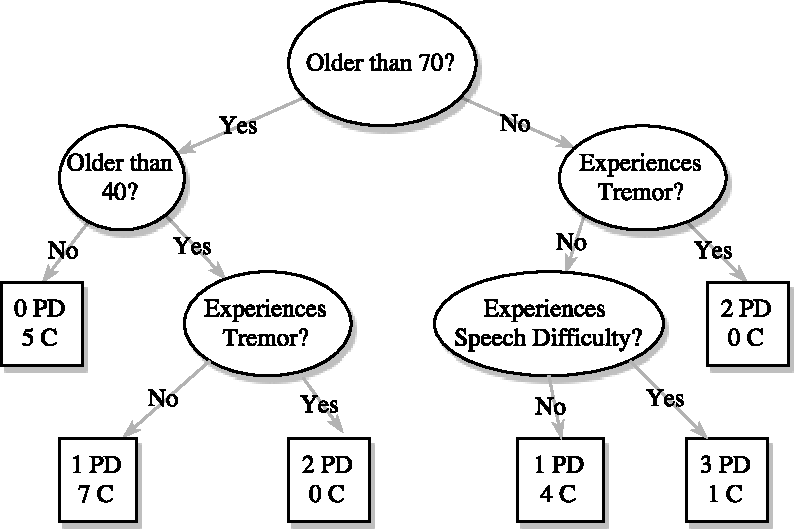
\includegraphics[width=0.7\linewidth]{decisiontree.pdf}
\caption{A simple Decision Tree with cutoff depth 3. Data is split by rules until a leaf contains only one class exists or a cutoff criterion is satisfied.}
\label{decisiontree}
\end{figure}

Decision Trees (\textit{\hyperref[decisiontree]{Figure}} \ref{decisiontree}) are robust against high dimensional data and their results are simple to interpret and transparent to human users (compared to SVMs and neural networks). However, selecting the optimal decision rules and cutoff criterion is a NP-complete problem. Decision rules are often developed based on greedy algorithms related to information criterion or search. A deep decision tree is prone to overfitting whereas a shallow one underfits.

Random Forests correct for the tendency of decision trees to overfit and offer robust and consistent results regardless of hyperparameters. The two hyperparameters are the number of trees to aggregate over and the number of features used in the search to split each branch of the tree. If the number of trees used is greater than the `complexity' of the problem, additional trees will not affect results~\cite{treesinaforest}. The square root of the number of features for classification is recommended by Breiman~\cite{randomforests} and performs well in most cases. Therefore, it is rare to perform hyperparameter tuning on random forests. In general, they are easier to interpret than SVMs and neural networks.

\begin{highlight}
Random forests provide robust and consistent results without the need for hyperparameter tuning.
\end{highlight}

\emph{Support Vector Machines}~\cite{svm} are built on the concept of creating the optimal decision boundary. The motivation is to create decision boundary which maximises the margin\footnote{The \emph{margin} is the smallest distance between the decision boundary and any of the samples} between different classes. A Lagrangian can be used to mathematically solve for a linear decision boundary. As most problems are not linear, the \emph{kernel trick} is used to transform the data into a linear space.


Kernels measure the similarity between two data points, and the kernel trick transforms the raw input into the feature space of the kernel\footnote{Kernels perform the same role as basis functions in linear regression}. Non-linear kernels enable a SVM to fit a non-linear function; however, selecting the perfect kernel is hard unless the exact non-linearity of the data is known. There are uncountably many kernels, and kernels such as the Radian Basis Function (RBF), Fisher and Polynomial are commonly used\footnote{There is rich literature in developing new kernels; however, these are rarely applied.}. Kernels also have adjustable parameters, such as the degree and constant coefficient for polynomial kernels. 

The original SVM algorithm was not able to handle cases where data was not separable. This led to the introduction of slack variables which define a penalty for data beyond the SVM's margins, extending their use to non-separable data~\cite{cortes1995support}. The sum of these slack variables is added to the SVM's Lagrangian equation along with a constant scaling factor $C$. The parameter $C$ balances the penalty for data beyond the margins with the size of the margin. A small $C$ is incentive to create a large margin whereas a large $C$ is incentive to minimise errors.

\begin{figure}[!htb]
	\centering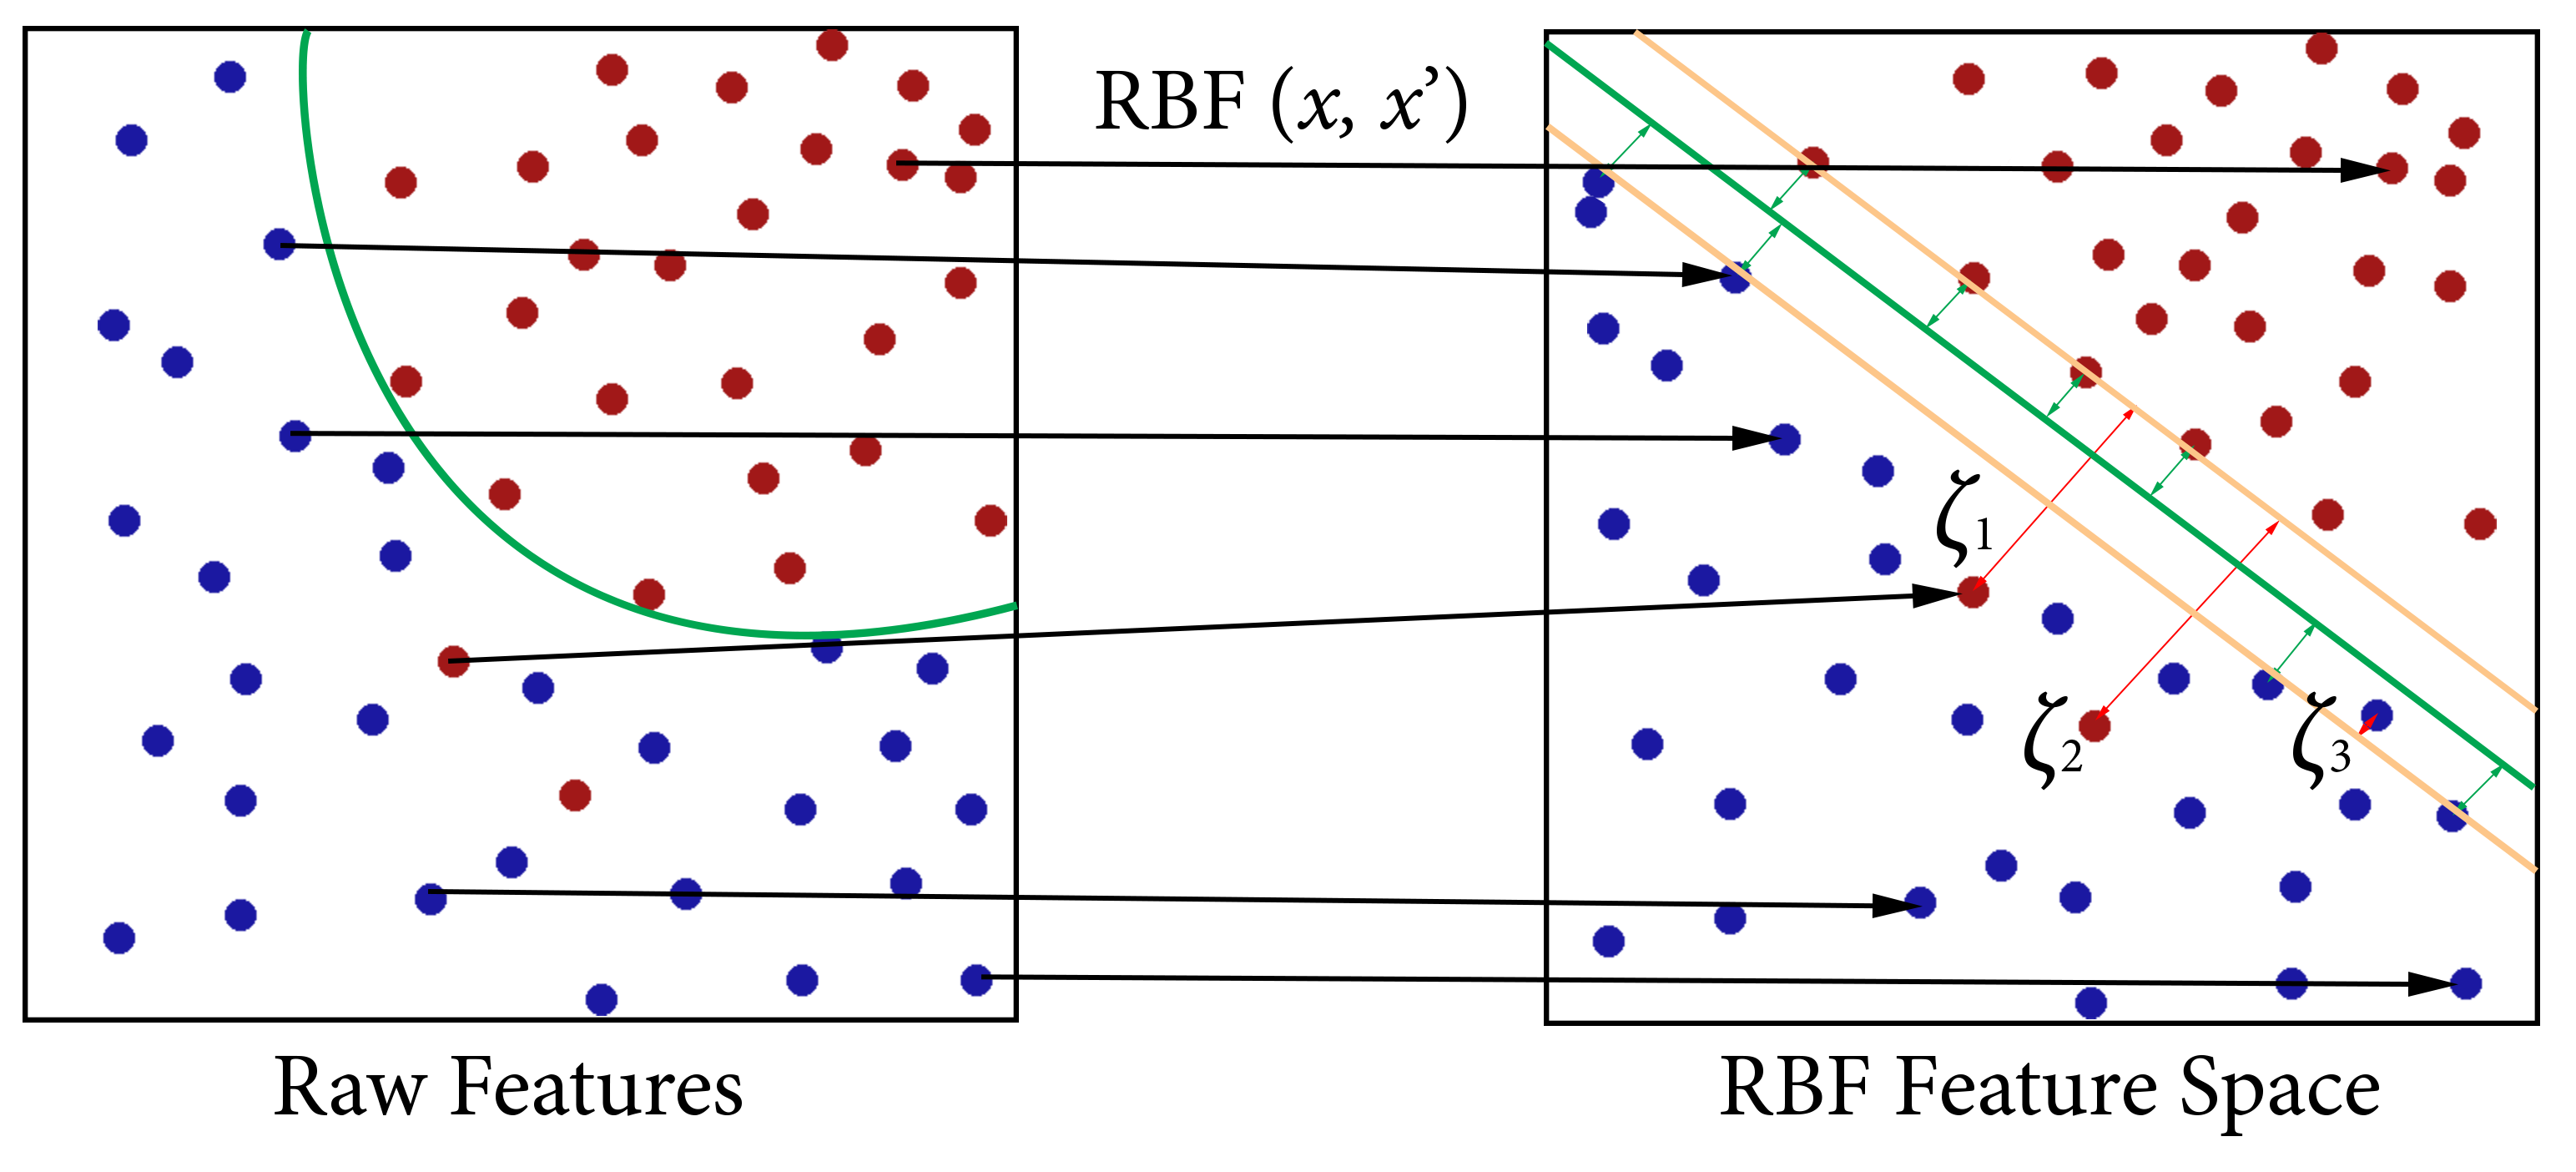
\includegraphics[width=0.8\linewidth]{svm.png}
	\caption{A RBF kernel is used to transform the data into a more linearly separable space. $\zeta_i$ denote slack variables which lie beyond the margin (depicted by beige lines). }
	\label{svm}
	\vspace{-0.5em}
\end{figure}
The combination of kernels and slack variables resulted in SVMs becoming popular in the machine learning community. A consequence of the improved performance is a reduction in interpretability --- making the SVMs a `black-box' method~\cite{svmblackbox} --- limiting its adoption in health care, where establishing user's trust through interpretable and easy-to-understand results is important. Kernels and slack variables also introduce many hyperparameters, such as the scaling factor $C$ and the type of kernel. Although intuition and knowledge of the data can guide kernel and hyperparameter choice, techniques such as grid or random search~\cite{gridsearch} are often used to fine-tune them. However, hyperparameter tuning increases the risk of overfitting, which will be discussed in \textit{\hyperref[detectoverfit]{Section}}~\ref{detectoverfit}. 

\begin{figure}[!htb]
	\centerline{\centering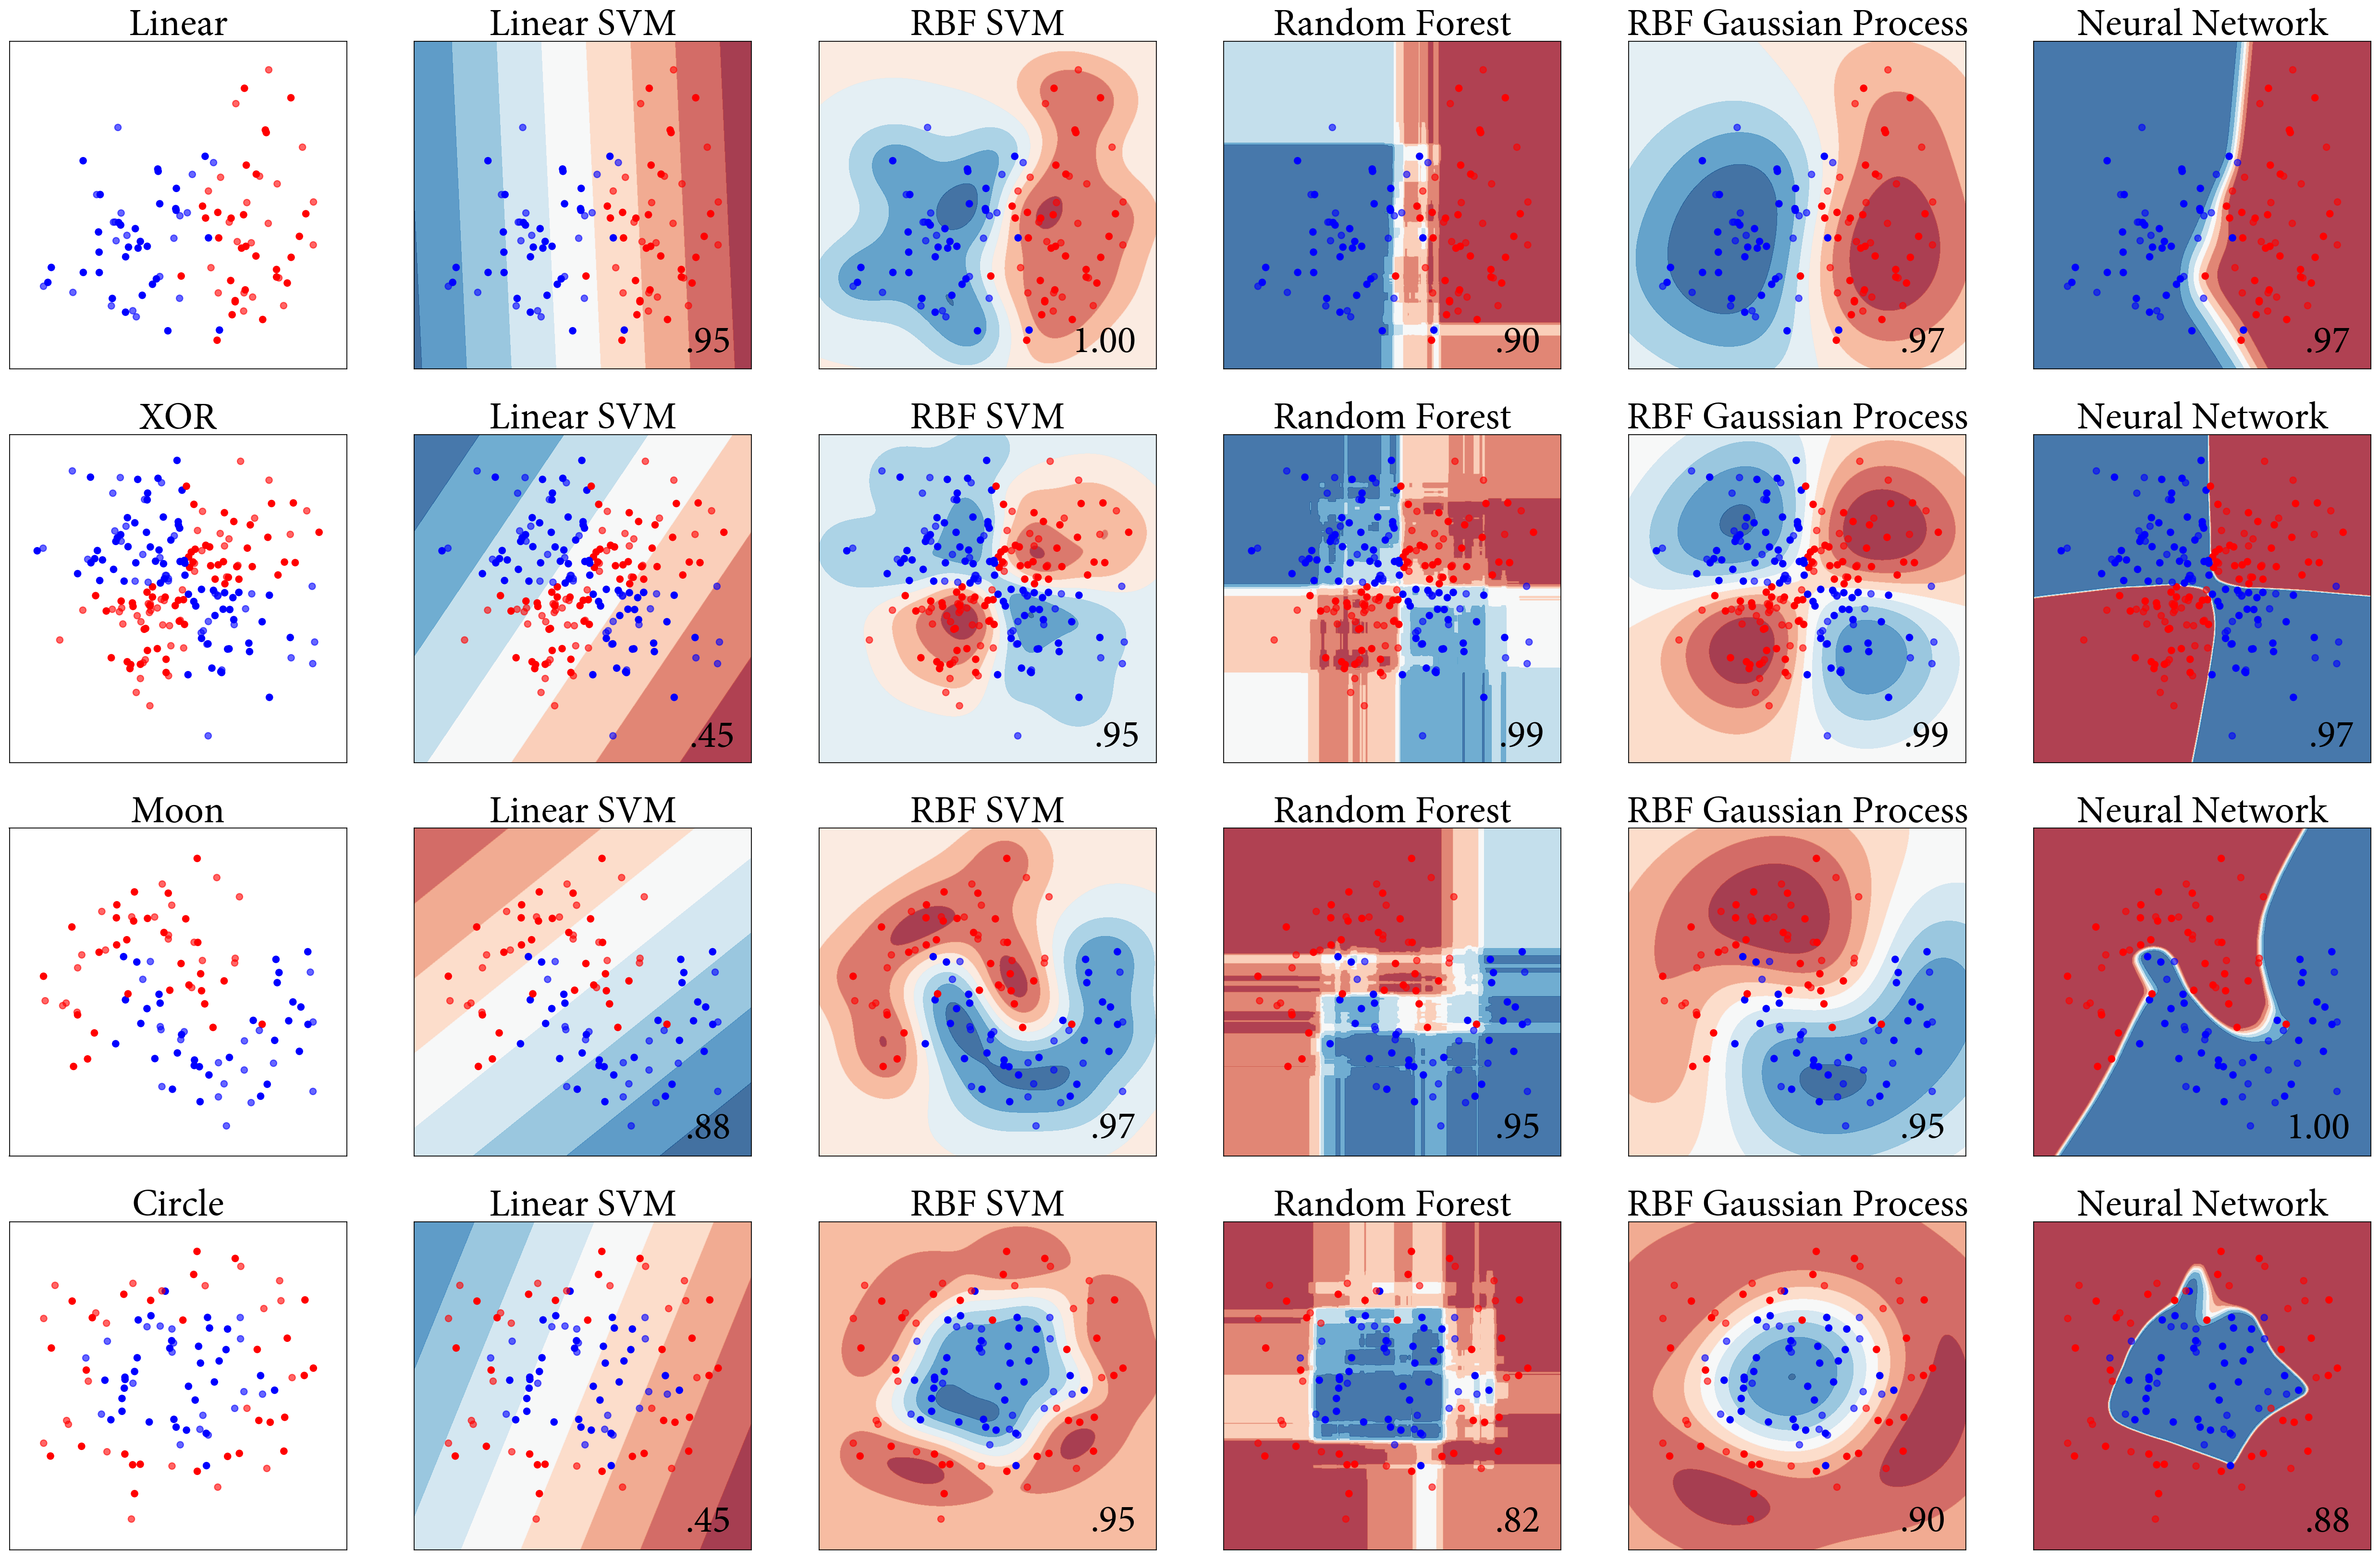
\includegraphics[width=1.2\linewidth]{model_vis.png}}
	\caption{A visualisation of various models ($x$ axis) fitting two dimensional distributions of data ($y$ axis). Choosing a model is difficult when the characteristics of the data are not well understood.}
	\label{modelvis}
\end{figure}

\subsection{Artificial Neural Networks}
%Most traditional machine learning models are derived under the assumption of independent and identically distributed data. The

%Random forests and SVMs are 
 
Traditional machine learning models perform best when data is structurally simple. Most statistical models such are designed to fit a linear function through the data, using pre-defined basis functions or the kernel trick to imitate non-linearity. Random forests and decision trees are powerful when data is readily available, but they do not model functions of data, and are less suitable when predicting unseen outliers~\cite{kramer2001propositionalization}. Neural networks are popular models used when the dataset is reasonably sized and there exists a complex structure between the input features. They are extremely powerful, but very difficult to interpret or debug; they are also highly prone to overfitting.
 
\label{neuralnetworkintro}Although neural networks have only recently risen to the spotlight, their history begins in 1943 with the introduction of a computational model of biological neurons\footnote{\emph{Neurons} are cells which transmit information via chemical and electrical signals. They are the fundamental building block of the human brain.}~\cite{nn1943}.
In 1958, the simple perceptron learning algorithm (\textit{\hyperref[perceptron]{Figure}} \ref{perceptron}) was developed~\cite{rosenblatt1958perceptron}, which would become the building blocks of neural networks today. The fundamental concept of a neural network is to connect many perceptrons (acting as neurons) together to simulate the behaviour of a biological brain. 



\begin{figure}[!htb]
\centering\includegraphics[width=1\linewidth]{perceptron.png}
\caption{The simple perceptron learning algorithm. The original incarnation could not handle inseparable data~\cite{rosenblatt1958perceptron}. Images adapted from Bishop~\cite{prml}.}
\label{perceptron}
\end{figure}

A perceptron by itself (\textit{\hyperref[perceptronvis]{Figure}} \ref{perceptronvis}) is a simple machine learning model, taking input features  and outputting a value representing a class or probability. As neurons were thought to have two states --- either firing or not --- the output was passed through a Heaviside\footnote{A discontinuous function which outputs either 0 or 1, defined as $ H(x)=\begin{cases} 
      0 & x < 0 \\
      1 & x \geq 0 
   \end{cases}
$} \emph{activation function}. At the time, computational power was limited, and large networks impossible to train. Early works by Minsky and Papert~\cite{minsky1969perceptrons} were misinterpreted as stating that perceptrons were incapable of modelling the `exclusive or' (XOR) function. However, Minsky and Pampert only proved this for a single perceptron and believed that multiple layers of perceptrons could model the XOR function. In 1989, it was shown that a single layer with enough perceptons can approximate any non-linear continuous function~\cite{nnuniversalapprox}.


\begin{figure}[!htb]
\centering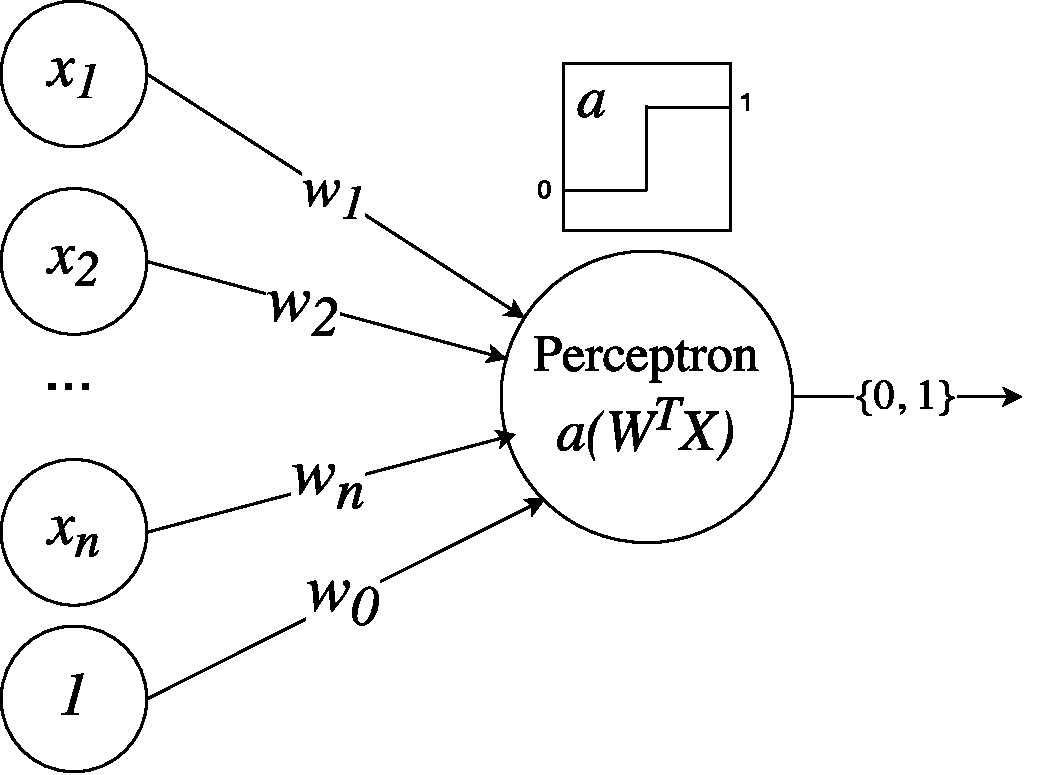
\includegraphics[width=0.5\linewidth]{perceptron.pdf}
\caption{A single perceptron node. Takes input $X$ and learns the weight vector $W$ to classify the output with the Heaviside activation function $a$.}
\label{perceptronvis}
\end{figure}

Multiple layers of perceptrons had always been the goal of neural network research; however, training them was not possible until backpropagation, a form of gradient descent\footnote{Surprisingly, Werbos' work on backpropagation~\cite{werbos1974beyond}  was lost and would be rediscovered a decade later in 1985 by Rumelhart et~al.~\cite{backproprediscover}} was developed~\cite{werbos1974beyond}. Backpropagation required the activation function to be differentiable, hence the sigmoid\footnote{The sigmoid function is defined as $\sigma(n) = \frac{1}{1+e^{-x}}$}  replaced the Heaviside activation function. Neural networks (\textit{\hyperref[nnetstacked]{Figure}} \ref{nnetstacked}) were now trainable, although computational power would be a bottleneck for a couple of decades. \textit{Deep learning} or \textit{Deep neural networks} are a general term for neural networks with many (generally more than 3) layers.

%. Unlike SVMs, a kernel does not have to be predefined - a neural network is able to learn a non-linear function of the data.

\begin{highlight}
A neural network's ability to learn complex non-linear relationships provides an advantage over traditional models, where this non-linearity must be defined.
\end{highlight}

\begin{figure}[!htb]
\centering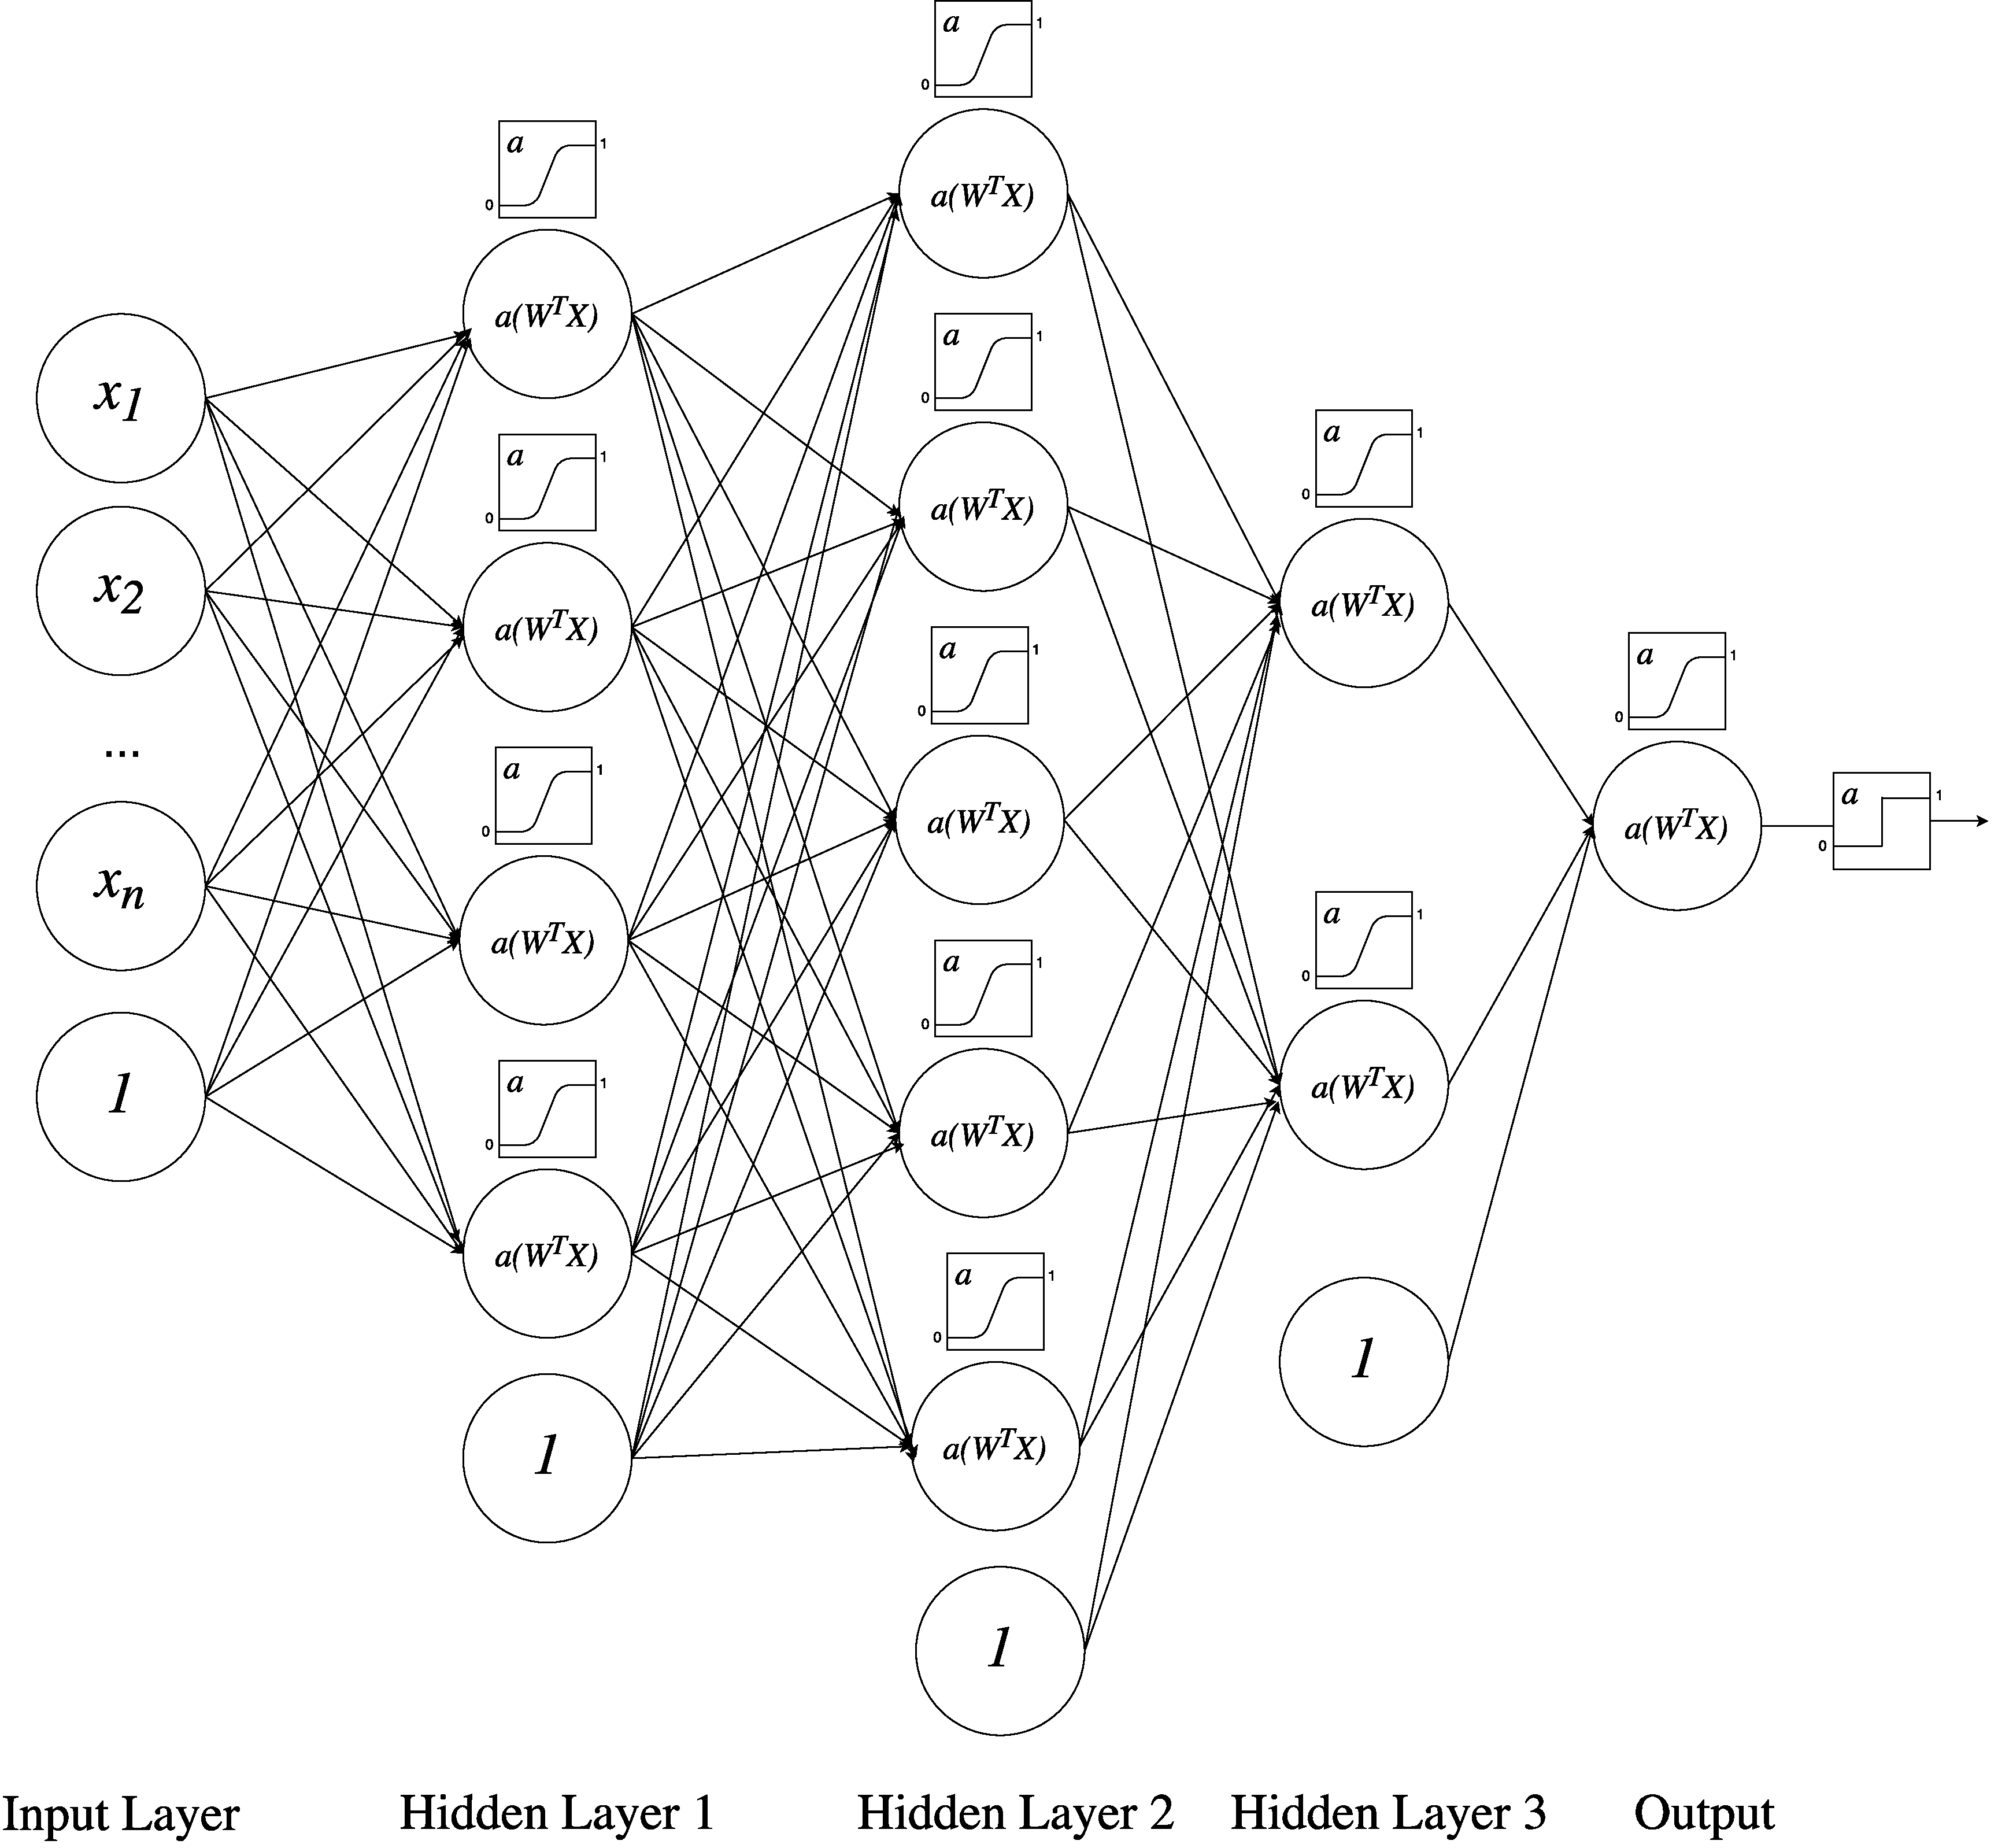
\includegraphics[width=1\linewidth]{neuralnet.pdf}
\caption{A simple\protect\footnotemark neural network with three fully connected hidden layers using sigmoidal activations. By stacking non-linear activation functions, neural networks are able to learn any non-linear function of the input. The '1' nodes represent the bias at each layer.}
\label{nnetstacked}
\end{figure}

\footnotetext{Typically, neural networks are more complex, consisting of more hidden layers, a variety of activation functions, and partial/structured connections.}


Neural networks are computationally expensive models and training them requires optimising a non-convex function. This is computationally intractable, so current neural networks use gradient descent and backpropagation to find a good local optima~\cite{convexopt}. The vanishing gradient problem~\cite{vanishinggradient} limited the depth of neural networks until the recent development of batch normalisation~\cite{batchnorm}. Previously, careful management of gradient flow was required to train deep neural networks~\cite{googlenet}. 

Two major variations of the traditional fully connected structure are convolutional and recurrent neural networks. Convolutional neural networks (\emph{CNNs}) are inspired visual cortex, where neurons are connected to local regions of the visual field. These networks contain `convolution' layers where neurons are connected to a small local region of neurons in the previous layer. These convolution layers learn a hierarchy of features (\textit{\hyperref[cnnvis]{Figure}} \ref{cnnvis}), and can negate the need for feature engineering for certain types of input data. Their power is clear in the task of image recognition, where CNNs have rapidly exceeded the performance of traditional models.


\begin{figure}[!htb]
	\centering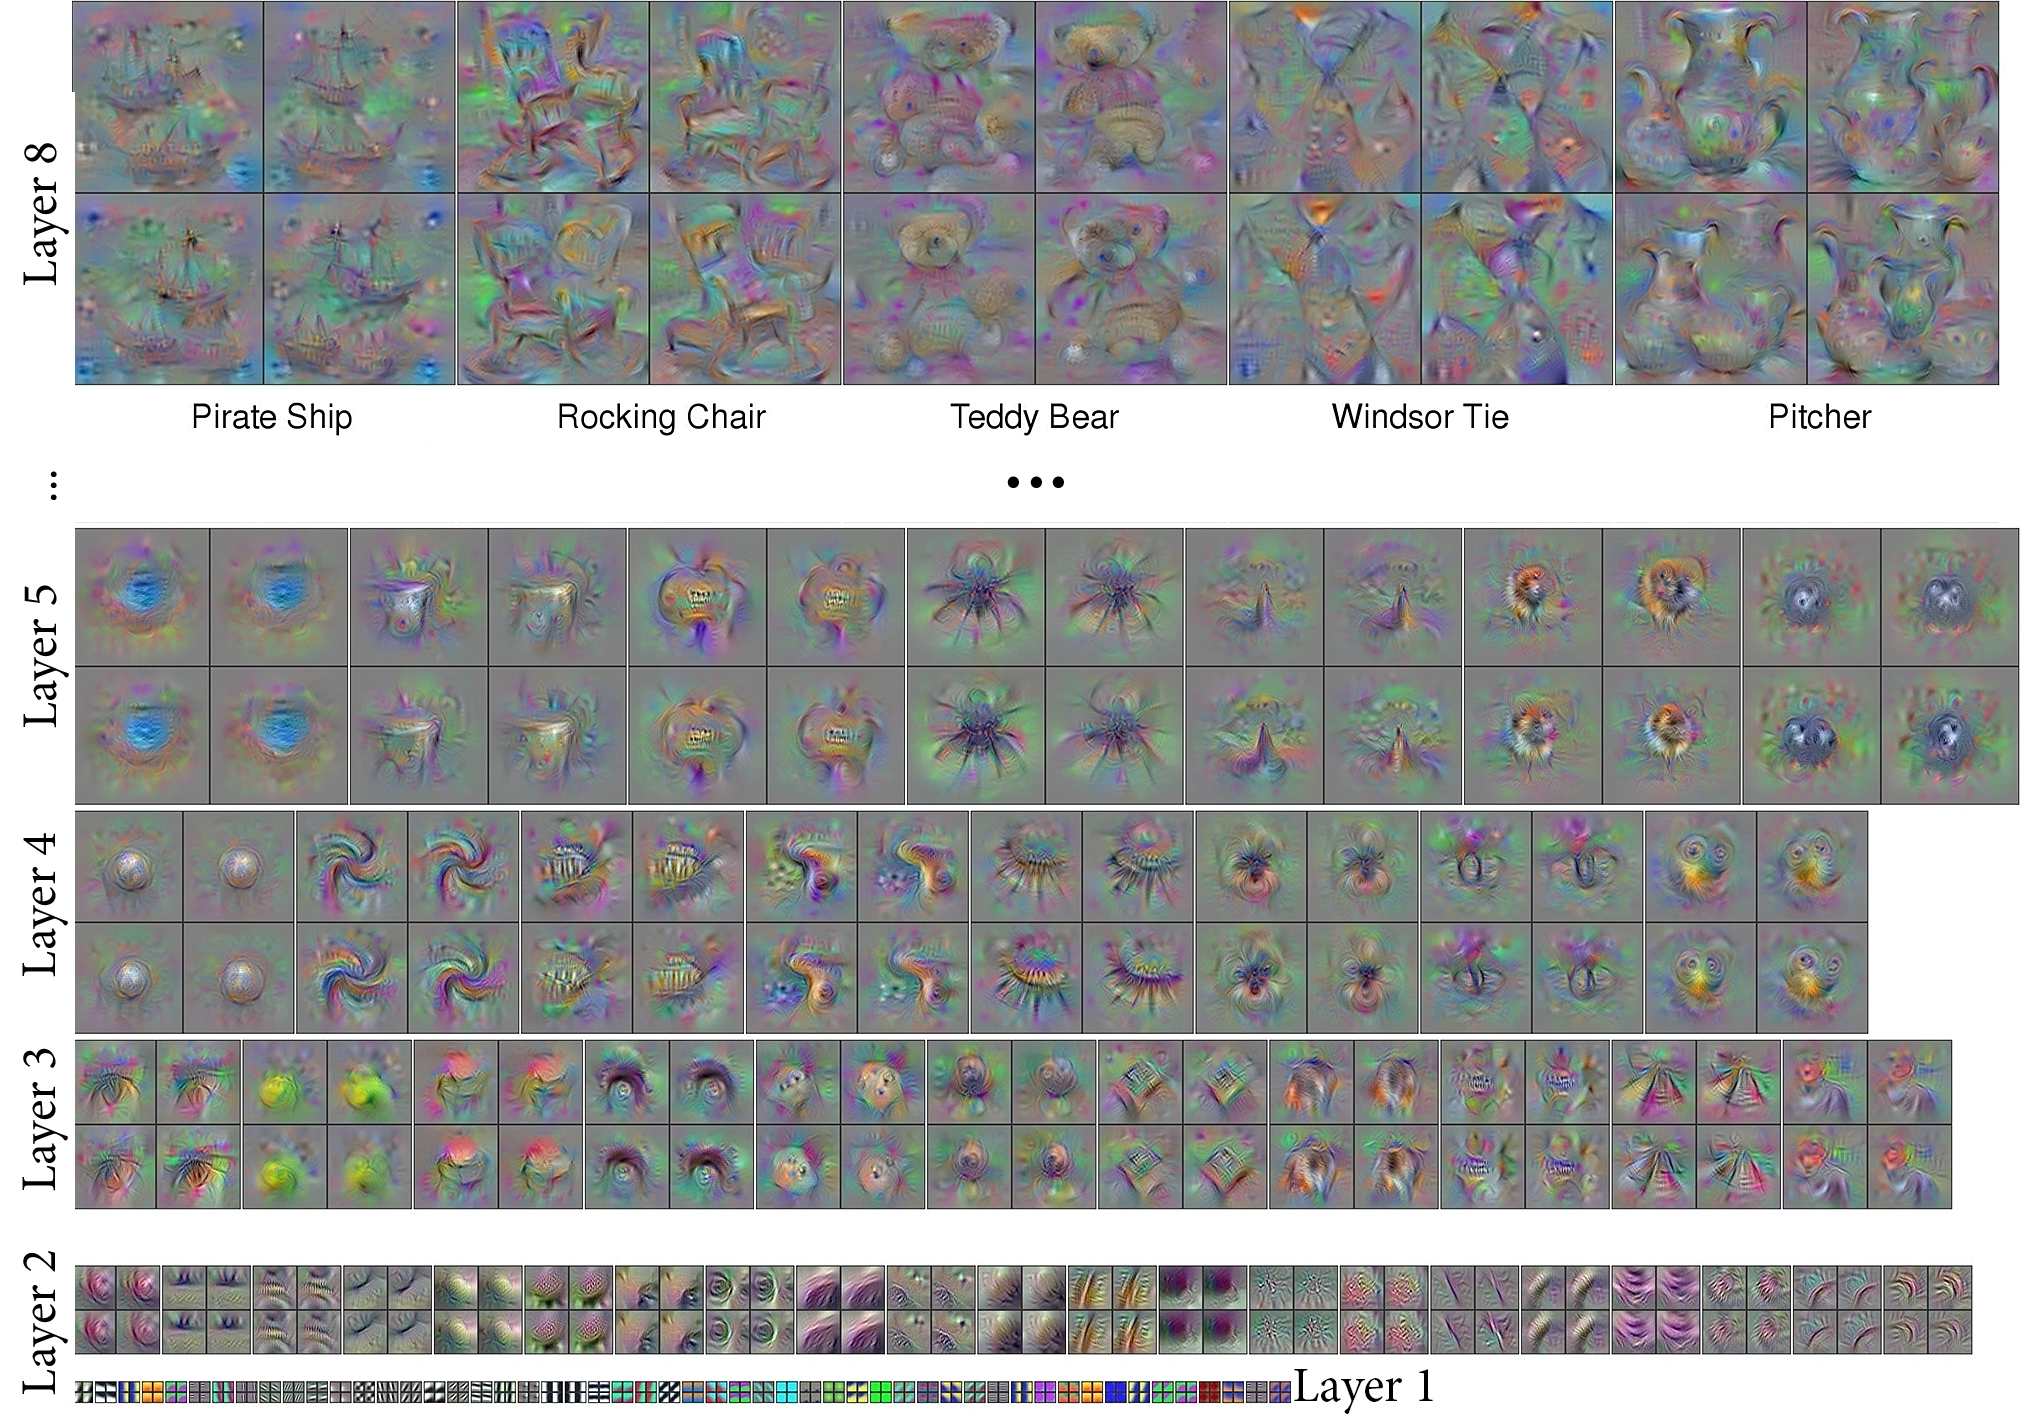
\includegraphics[width=1\linewidth]{cnnvis.png}
	\caption{A visualisation of CNN activations from Yosinski et al.~\cite{cnnvis}. Layers capture increasingly complex relationships between pixels and are input features to further layers. }
	\label{cnnvis}
	\vspace{-0.4em}
\end{figure}


Recurrent neural networks (\emph{RNNs}), on the other hand, have cyclic connections. This simulates an internal state which allows RNNs to base future predictions on past data, therefore better handling temporal information. There are a number of RNN variants, and long short-term memory (LSTM) nodes are the most common in practice as they are more robust to the vanishing gradient problem~\cite{lstm}. Recently, fusion models of LSTM and convolution layers have seen success in EEG classification~\cite{bashivan2015learning} and multimodal activity recognition~\cite{deepconvlstm}.
%RNNs also and provides flexibility for the type of input and output data. 


\subsubsection{Neural Network Hyperparameters}
Neural networks have many hyperparameters --- combined with computationally expensive training, hyperparameter tweaking often relies on intuition. This section will provide a basic intuition behind selecting hyperparameters of a neural network. 

The most fundamental features are the width and depth of the network. In general, increasing the number of nodes in a network reduces its bias and is effective when data is plentiful. It is thought that networks with many nodes per layer (\emph{width}) are better at memorization, while additional layers (\emph{depth}) are better at generalisation of features~\cite{cheng2016wide}. Depth can also be exponentially more valuable than width for modelling the structure of complex non-linear data~\cite{eldan2016power}. There is still no consensus on the balance between number of nodes and layers --- this varies significantly problem to problem.

A large neural network tends to overfit by memorising the data. Regularisation is a method of preventing this without reducing the size of the network. In traditional machine learning, $l_1$ and $l_2$ weight regularisation is most common. This involves adding a penalty to weights, motivated by Occam's razor where a simpler model (smaller weights) is preferred. When applied to neural networks, weight regularisation slows convergence and complex models can still be learned with a deep enough network. {Early stopping} and {dropout} are the most common forms of regularisation in practice.
\newpage 

\emph{Early stopping} involves stopping training before the optima is reached, at the point where the cross-validation accuracy starts to decrease from overfitting. \emph{Dropout} involves randomly disabling some percentage of nodes on each layer at each iteration of gradient descent~\cite{dropout}. This may appear unintuitive; however, the motivation is to promote redundant feature representations to improve its robustness. Dropout and early stopping are a powerful combination and used in most architectures. There are also variations of dropout such as dropconnect~\cite{dropconnect} where connnections rather than nodes are zeroed.

A major problem with the sigmoidal activation function is that as the activation approaches either 0 or 1 the gradient approaches zero. This is known as \textit{saturation} and significantly slows the convergence of gradient descent in the training process. Rectified linear units (\emph{ReLUs}) use the activation function $f(x) = \max(0,x)$ which resolve the gradient issue and are believed to be more biologically plausible~\cite{relu,relubiology}. One notable characteristic of ReLUs is that once the unit outputs zero, it is essentially `dead' as the gradient of the rectifier is zero. A number of modifications to ReLU have been proposed such as the leaky/parametric ReLU~\cite{heinitialization} ($f(x) = \max(\alpha x, x)$ for $\alpha\leq 1$), Maxout~\cite{goodfellow2013maxout}, noisy ReLU~\cite{relu} and exponential linear unit~\cite{clevert2015fast}.

The initialisation of the weights in the network will affect the solution found by gradient descent and the rate of convergence to it. Poor initialisation can result in the death of ReLUs or saturation of sigmoidal and tanh units. Recently, it was shown that initializing the weights according to a Gaussian distribution with variance $2/(n_{\text{in}}+n_{\text{out}})$, where $n_{in}$ is the number of inputs to the node and $n_{out}$ the number of outputs was highly effective in preventing saturation. This is termed Xavier or Glorot initialisation and is effective for networks with sigmoidal or tanh activations~\cite{glorot2010understanding}. However, Xavier initialisation causes ReLUs to rapidly tend to zero, so small modification was proposed where variance is set to $2/n_{\text{in}}$, termed He initialisation~\cite{heinitialization}.

The method of gradient descent, referred to as the \textit{optimiser} is also a major area of neural network research. Traditional gradient descent often gets stuck at saddle points and local minima as the gradient is zero, as depicted in \textit{\hyperref[graddescent]{Figure}} \ref{graddescent}. Non-linear techniques developed in convex optimisation such as conjugate gradient descent and (Quasi-)Newton methods are powerful, yet rarely applied in practice due to their computational complexity. The most popular optimisers for neural networks incorporate the concept of momentum, where earlier gradients are considered in the descent. Adam~\cite{adam} is one of the most recent optimisers and combines elements from two powerful optimisers before it, AdaGrad and RMSProp. Nesterov momentum~\cite{nesterov1983method} --- which has favourable properties in convex optimisation --- can also be incorporated into Adam, creating Nadam~\cite{nadam}. 

\newpage
\begin{figure}[!htb]
	\centering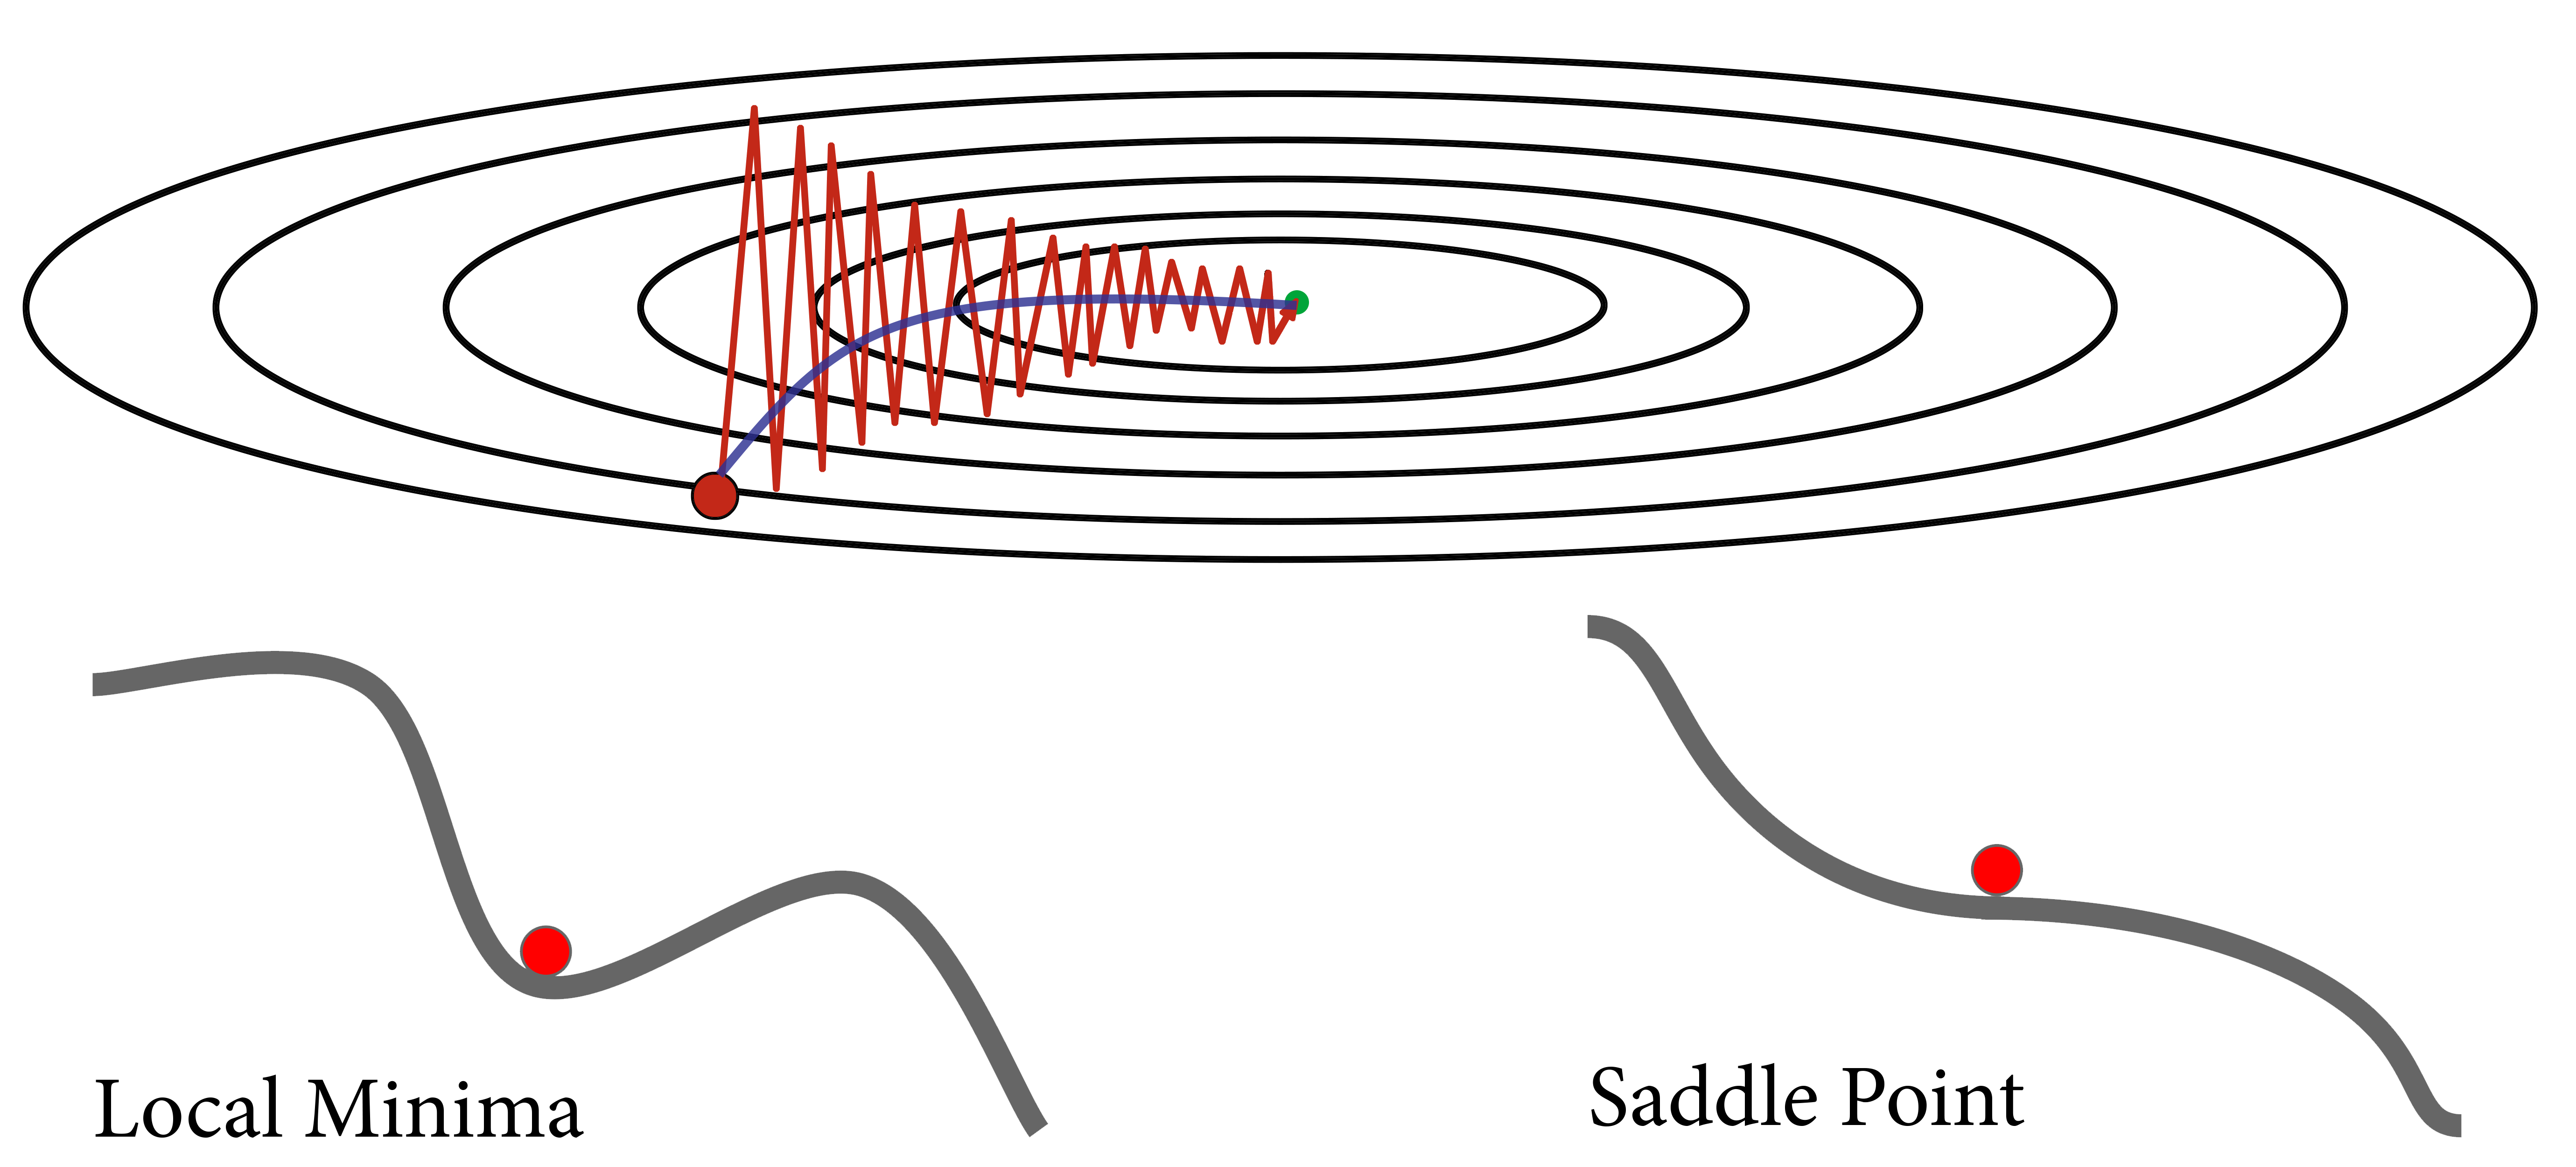
\includegraphics[width=0.82\linewidth]{gradescent.png}
	\caption{Traditional gradient descent (red curve) performs poorly in `long valleys'. Optimisers generally use momentum to simulate the behaviour of the optimal blue curve and avoid local minima. Diagram adapted from Stanford's CS231n~\cite{cs231n}.}
	\label{graddescent}
\end{figure}

Each optimiser also has its own hyperparameters, the most major one being the learning rate. As training is stochastic, training multiple models and using them in an ensemble often results in better performance. Loshchilov and Hutter~\cite{sgdrestarts} proposed a novel approach where the learning rate is fluctuated during training to create multiple different models to ensemble in one training process. 

\vspace{1em}

\subsection{Feature Selection and Dimensionality Reduction}
\label{fseldimred}
The general approach to a machine learning problem is to extract as many features as possible then decide which are most relevant. Redundant or highly correlated features reduces the performance of most machine learning algorithms. Simple models like Na\"{i}ve Bayes rely on the assumption that features are independent and correlated features can disproportionately weigh certain factors. Neural networks are better equipped to handle correlated and redundant features; however, may need more data and training time to do so. 


%\footnote{There are issues with this approach such as Freedman's paradox~\cite{freedmanparadox} however resolving this is the task of model evaluation (Section \ref{detectoverfit}).}

\begin{highlight}
	Feature selection techniques aim to eliminate useless features and dimensionality reduction reduces the correlation between features.
\end{highlight} 

\emph{Feature selection} simplifies the model by selecting a subset of features to use. This increases the interpretability of a model, reduces the probability of cross-validation overfitting~\cite{overfittingcv} and speeds up training. Selecting the optimal subset of features is not a simple task as some features may be uninformative on its own, but useful when combined with others. An computationally intractable exhaustive search would be required to determine the optimal subset. Feature selection algorithms aim to quickly find a good subset and can be categorised as filters, wrappers and embedded methods. 

\emph{Filters} evaluate subsets of features by maximising various criteria such as entropy, similarity and other statistical measures. Evaluation of subsets are fast and results are independent of machine learning model. However, a majority of filters are based on the assumption of linearity, and may not be suitable when complex relationships exist between features. \emph{Wrappers} `wrap' around existing models, using cross-validation to evaluate a feature subset. Features are therefore better tailored to each model; however, wrappers may be computationally prohibitive and also cater towards the model's tendency to overfit~\cite{wrapperoverfit}. \emph{Embedded} methods are based on models which inherently perform feature selection during their training, often from strong regularisation. 

The performance of these approaches are highly domain-dependent. This thesis employs state of the art supervised feature selection algorithms as depicted in \textit{\hyperref[featureselection]{Table}} \ref{featureselection}.  We refer to Li~et~al.~\cite{skfeature} for a thorough description and comparison of chosen techniques. 

\begin{table}[!htb]
	\caption{Feature selection methods used in this thesis. Implemented with scikit-feature~\cite{skfeature}}
	
	\label{featureselection}
	\centering
	\begin{tabular}[t]{c c c}
		\toprule
		{\specialcellbold{Filter}} &
		{\specialcellbold{Wrapper}} &
		{\specialcellbold{Embedded}}\\
		\midrule
		
		\begin{tabular}[t]{@{}l@{}}ReliefF~\cite{relieff}\\ 
		Fisher score~\cite{fisherscore}\\
		CIFE~\cite{cife}\\
		JMI~\cite{cife}\\
		ICAP~\cite{icap}\\
		MIFS~\cite{cife}\\
		MRMR~\cite{mrmr}\\
		CFS~\cite{CFS}	
		\end{tabular}
		& 
		
		\begin{tabular}[t]{@{}l@{}}SVM/Gaussian Process\\
			Forward/Backwards\\
			Search
		\end{tabular}
		&
		\begin{tabular}[t]{@{}l@{}}RFS~\cite{fs_rfs}\\
			ls\_l21~\cite{l21}
		\end{tabular}	
		\\
		\bottomrule
	\end{tabular}
\end{table}

Rather than eliminating features, \emph{dimensionality reduction} reduces the amount of information required to represent the set of features. This can de-correlate features and improve performance for simpler machine learning models. The two most common forms of dimensionality reduction are the unsupervised principal component analysis (PCA) and supervised linear discriminant analysis (LDA)~\cite{prml}. Neural networks can also be used to reduce the dimensionality of data by training a network to predict the input, where layers progressively contain fewer nodes. These are termed autoencoder networks and can out-perform PCA; however, they are more difficult to analyse~\cite{nndimred}.	 


\begin{highlight}
Feature selection is almost a requirement for small datasets, whereas dimensionality reduction is less commonly applied as it can obfuscate the model. 
\end{highlight}
\newpage
\subsection{Model Evaluation and Handling Overfitting}
\label{detectoverfit}
The primary goal of machine learning is to train a model which will generalise well to new data. Accuracy over the entire dataset is evidently not a good metric, as a model which memorises the data (overfit) can appear to have perfect accuracy while failing to generalise to new data. Model selection and evaluation is the field in statistics which handles this. 

Cross validation (\emph{CV}) has become the de-facto standard in machine learning. Conceptually, CV is simple --- the primary types used in machine learning are \textit{leave-one-out} and \textit{k-fold}. Let there be 100 data points in a dataset. In leave-one-out CV (LOO-CV), 99 data points are used to train a model, and 1 data point to test and evaluate the performance. This is repeated over each  data point and the average result taken as the generalization accuracy. K-fold is similar; however, rather than using only one data point, the data is split into $k$ groups, training on $k-1$ and testing on $1$ group. For example, 2-fold CV involves training on group 1 and testing on group 2 then training on group 2 and testing on group 1. CV reduces the risk of overfitting; however, repeated runs of CV over different models increases the probability of overfitting.



\begin{highlight}[Model Selection]
	Good model selection techniques are becoming increasingly important in machine learning as improvements become more marginal, and are likely to arise from natural variance in an model~\cite{overfittingcv}.
\end{highlight} 



In summary, we will be performing 10-fold CV with random stratification\footnote{\emph{Stratification} involves ensuring there are an equal ratio of classes in each group. In this case, people with and without PD. } repeated 10 times. This results in a set of 100 accuracy values after taking the mean accuracy of each fold of cv for each model. The same stratification sets are used, and Bayes factor~\cite{bayesianttests} is used to test if the mean performance of one model is greater than the other. This decision will be justified in the following section with more background into model selection and hypothesis testing provided.

\subsubsection{Model Selection and Hypothesis Testing }

K-fold CV and LOO-CV are the de-facto standards in machine learning, and it is rare to look for alternatives. They provide a good estimate for generalisation error, are easy to implement and fast to evaluate. LOO-CV allows almost all the data to be used in training. When the data is clean (high signal-to-noise ratio) LOO-CV performs nearly unbiased estimations~\cite{crossvalsurvey}. However, LOO-CV has been criticised for preferring models with a high variance and is less computationally feasible for large data sets~\cite{kohavi1995study}. Kohavi~\cite{kohavi1995study} instead recommends 10 fold CV in the general case. CV variations such as exhaustive and Monte-Carlo CV exist, but are not recommended by statistical literature~\cite{kfoldvsloo, crossvalsurvey}. 

There are a number of catches when performing cross validation. Importantly, CV requires validation data to be independent from training data. In medical contexts, it is common to have multiple recordings from a single patient. Recordings from the same patient are likely to share similar attributes and cross-validating na\"{i}vely over the whole dataset can easily overfit~\cite{mpowerneto2017analysis}. Secondly, when performing hyperparameter optimisation the CV score is used as a metric. This introduces the risk of the best model hyperparameters fitting the validation sets by chance~\cite{overfittingcv}.

Overfitting on cross-validation is difficult to detect without additional data and is a major issue in small datasets. A common approach is to take a subset of data as the `test' data which remains unseen in hyperparameter optimisation; however, this is infeasible when there is not enough data to create a test set large enough for results to be meaningful. Ng~\cite{overfittingcv} proposes an algorithm to select from a number of competing hypothesis. Repeating k-fold CV with different division of folds can also reduce the likelihood of overfitting on CV by chance. Bouckaert~\cite{bestcvempirical} recommends 10 fold CV repeated 10 times after extensive empirical testing.

Accuracy is the most basic and intuitive measure of performance; however, it has been the subject of a number of criticisms. Firstly, it is susceptible to the false positive paradox\footnote{The false positive paradox occurs when there is a very low incidence of a positive results in the target population. For example, when only 1 per cent of the population suffer from PD, a model which only predicts `no PD' will be completely uninformative yet perform better than any model which predicts PD sometimes.}, and may not be a good representation of a model's effectiveness in difficult tasks. Sensitivity, or recall, is a measure of the proportion of positive classes correctly identified and specificity measures the proportion of correctly identified negative examples. Precision is occasionally used instead of specificity in the machine learning community, measuring the proportion of correctly identified positive examples over all positive predictions. The $F_1$ score is the harmonic mean of sensitivity and precision and is an more effective measure of model performance when classes are unbalanced. 


Secondly, accuracy does not take into consideration the confidence of a model's predictions. The area under the ROC (Receiver Operating Characteristics~\cite{rocauc}) curve (\emph{AUROC}) was proposed as a better alternative to accuracy. The ROC curve is created by plotting sensitivity and specificity at all confidence thresholds, and the area under ROC was believed to be a more robust and consistent measure of model performance~\cite{aucgood}. However, recent empirical experiments have shown that AUROC favours particular models~\cite{aucmislead2} and it has been criticised for being incoherent~\cite{aucmislead, aucincoherent}. Modifications to AUROC have been proposed~\cite{aucmislead2, aucincoherent}, but they are uncommon in practice. As a result, accuracy will be the primary performance measures utilised in this thesis as it is interpretable and independent of model characteristics. AUROC is more robust when there is a large disparity between classes, and will also be recorded for comparison with prior works such as Neto et~al.~\cite{mpowerneto2017analysis}.


\begin{table}[!htb]
	\caption{A summary of common performance measures used in machine learning and statistics literature.}
	\label{measuremeaning}
	\centering
	\begin{tabular}[t]{c c c}
		{\specialcellbold{Confusion Matrix}} & &
		{\specialcellbold{Measure Definitions }} \\[10pt]
		\begin{tabular}{lcl}\hhline{~|*{2}{-}}
			\multicolumn{1}{l|}{}                                 & \multicolumn{1}{c|}{\cellcolor[HTML]{EFEFEF}Pred True} & \multicolumn{1}{c|}{\cellcolor[HTML]{EFEFEF}Pred False} \\ \hline
			\multicolumn{1}{|l|}{\cellcolor[HTML]{EFEFEF}\specialcell{Real\\True}} & \multicolumn{1}{c|}{\specialcell{True Positive\\ (TP)}}                          & \multicolumn{1}{c|}{\specialcell{False Negative\\ (FN)}}                         \\ \hline
			\multicolumn{1}{|l|}{\cellcolor[HTML]{EFEFEF}\specialcell{Real\\False}}  & \multicolumn{1}{c|}{\specialcell{False Positive\\ (FP)}}                          & \multicolumn{1}{c|}{\specialcell{True Negative\\ (TN)}}                         \\ \hline
			
		\end{tabular}
		& &
		\begin{tabular}{@{}rc@{}}
			\specialcellright{Sensitivity\\ \hspace{1.6em}/Recall}    & $\dfrac{TP}{TP+ FN}$      \\ \midrule
			Specificity  &   $\dfrac{TN}{FN+FP}$   \\ \midrule
			Precision &    $\dfrac{TP}{TP+FP}$  \\ \midrule
			$F_1$ Score    &   $\dfrac{2TP}{2TP + FP - FN}$   \\ \midrule
		\end{tabular}
	\end{tabular}
\end{table}

Hypothesis tests are used to determine if the results obtained in experiments are \textit{statistically significant}. After cross validation, a hypothesis test should be used to determine that the difference in results is not by chance. Paired t-tests are the traditional approach; however, they have been subject to a range of criticisms regarding replicability~\cite{publicationbias, replicability}. Recently, the American Statistical Association has officially endorsed \textit{Bayes factor}~\cite{bayesianttests} (\emph{BF}) as their preferred method of hypothesis testing~\cite{bayesfactorASA}. Mass-replication studies have shown that almost a half of prior psychological research does not meet the criteria for strong evidence when Bayes factor is applied~\cite{bayesfactorempirical}. Their interpretation is depicted in \textit{\hyperref[bayesfactorinterpretation]{Figure}} \ref{bayesfactorinterpretation}. The standard two tailed Cauchy distribution is used as a prior in this thesis~\cite{bayesianttests}.


\begin{table}[!htb]
	\caption{Interpretation of Bayes factors~\cite{bayesfactorinterpretation}. Bayes factors do not account for model validity and selection bias.}
	\label{bayesfactorinterpretation}
	\centering
\begin{tabular}{@{}rc@{}}
	$<1$ &  Evidence for the null hypothesis of $1/BF$\\ \midrule
	1 to 3 &  Insignificant evidence\\ \midrule
	3 to 10 & Substantial evidence \\ \midrule
	10 to 30    & Strong evidence    \\\midrule
	30 to 100 & Very strong evidence\\\midrule
	$\geq 100$ & Decisive evidence \\\midrule
\end{tabular}
\end{table}


Consider three models: $A$ which achieves 80 per cent accuracy, $B$ at 81 per cent and $C$ at 81 per cent. $B$ is strictly dominant to $A$, correctly classifying all of $A$'s successes and additionally some of its failures. $C$ has a very different set of successes and failures to $A$. Our Bayesian approach to model selection distinguishes the two cases, with $B$ obtaining the more significant result than $C$, as it is more likely due to an improvement in the model rather than chance. 

In statistics, there is no agreed upon method for model selection and evaluation. Penalization based evaluation\footnote{\emph{Penalization} based model criteria are inspired by Occam's razor, preferring simple models over complex ones which as they are less likely to overfit. A penalty is attached to the number of free parameters in a model.}  criteria such as Akaike/Bayesian/General Information Criterion~\cite{aicbic,generalinfocriteriongic} and Minimum Description Length~\cite{mindescriptionlength} are common model selection techniques. However, these are less suitable for machine learning as it is difficult to quantify the complexity of model such as neural networks. Cross validation is therefore the only feasible technique to compare completely different models. 
 

Overall, it should be clear that results reported in machine learning are highly susceptible to overfitting and should be considered with a grain of salt. Unless standard datasets of an substantial size are developed, methodology rather than results should be the primary concern. Seemingly insignificant details such as stratifying on a per-person or a per-sample level can be the difference between an AUROC of 98 and 45 per cent~\cite{mpowerneto2017analysis}. 

Cross validation results should not be interpreted as real-world generalisability --- especially in small datasets. Accuracy will undoubtedly increase in the future when more training data becomes available. Furthermore, there is no statistical technique which can reliably account for inherent bias in the dataset or flawed methodology.

%Dieterrich recommends two fold, understimate variance ~\cite{bestcvapproximate}
%\cite{nounbiasedkfoldcv}




\chapter{Our Work}
\label{ourwork}
\vspace*{-1em}
Although there is a rich selection of prior work in PD diagnosis with machine learning, the lack of a standard dataset and methods limits the comparability of different studies. It is apparent that multiple sub-fields exist and research is often confined within its own sub-field. For example, the top papers in the Interspeech 2015 PD speech challenge~\cite{compareis15pd} used methods independent of the dysphonia feature engineering previously done for PD. Research also rarely considers the results of works completed in challenges such Interspeech or Michael J. Fox Foundation Parkinson's data challenges~\cite{mjfoxchallenge2013}. It is common to find papers failing to cite prior work which performs the same experiments. A major goal of this thesis is to consolidate and distil the techniques applied in prior works in a coherent, sequential format.

\begin{highlight}
Multiple sub-fields exist in PD literature and research is often isolated within a sub-field.
\end{highlight}

Although prior works have reported excellent results, it is difficult to determine if these results are caused by biases in the dataset or overfitting. Like any field based on empirical statistics, a publication bias exists~\cite{publicationbias}, and there will exist irreproducible results~\cite{replicability}. \textit{\hyperref[detectoverfit]{Section}} \ref{detectoverfit} details measures such as significance testing to reliably evaluate and select models; however, their implementation is uncommon in machine learning literature. 

The variation of results shines doubt on the replicability of the best performing papers. Arora~et~al.~\cite{arora2014high} achieves 98 per cent accuracy using smartphone IMU data from 20 participants. In contrast, Zhan~et~al.~\cite{zhan2016high} uses all features in Arora~et~al., in addition to speech and tapping measures; however, only manages 71 per cent accuracy. Furthermore, state of the art techniques in motion mode recognition rarely achieves such results, despite motion mode recognition likely being the `easier' task~\cite{motionmoderecognition}. 

Neto et~al.~\cite{mpowerneto2017analysis} shows that it is possible to ``digitally fingerprint'' people using accelerometer and voice data, and that failure to split data on a per-participant scale is subject to overfitting. The walk signal was very informative at classifying PD when split at the sample level (AUROC $\approx 98$ per cent) and uninformative when samples were split at a participant level (AUROC $\approx 45$ per cent). 
 \newpage
%The following sections detail the experiments performed as part of the project. %To reduce the risk of overfitting and bias, we have employed a much larger, albeit `noisier' dataset.

%We will apply a combination techniques used in state of the art on a larger dataset to assess true performance. The mPower dataset~\cite{mpower} has been chosen for this  task and will be described in the following section.


\section{The mPower Dataset}
\label{mpower}
To minimise the likelihood of bias or overfitting, a larger dataset was required. Currently, the only publicly available dataset that satisfies this requirement is mPower~\cite{mpower}. 

\begin{figure}[!htb]
\label{mpowerapp}
\centering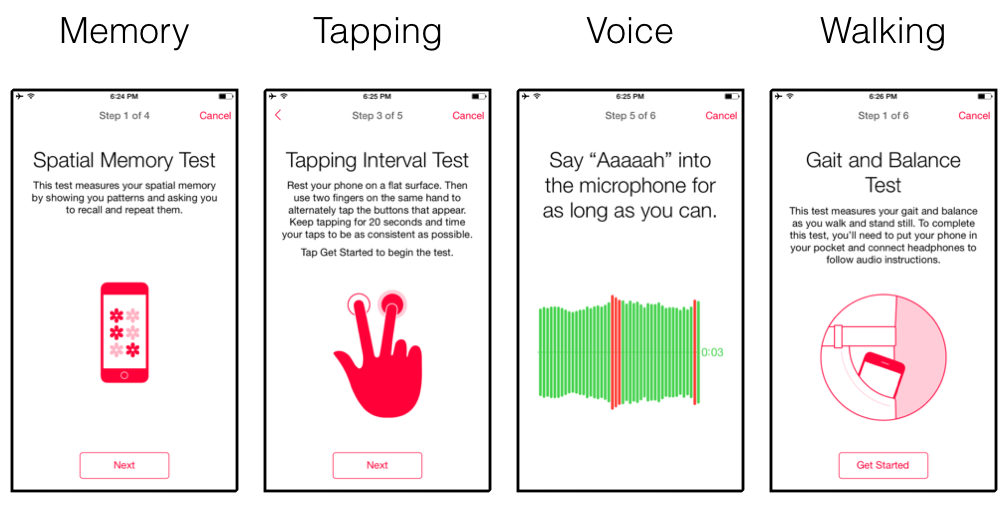
\includegraphics[width=1\linewidth]{mpower.png}
\caption{The mPower app consists of several tasks to evaluate memory, bradykinesia, voice and gait. }
\end{figure}

The mPower study began in March 2015, open to people living in the United States who owned an Apple iPhone or iPod released in 2011 or later. Upon downloading the app, the user is presented with the tasks depicted in \textit{\hyperref[mpower]{Figure}} \ref{mpower}, along with general demographics and UPDRS questions. Each task/questionnaire was optional and could be completed multiple times. As of writing, there are around 6,500 participants in the study, 1,100 with PD. Users come from diverse backgrounds and may have other illnesses. The mPower dataset also contains a number of cases of young-onset Parkinson's disease\footnote{Assuming the participants are honest of their circumstances.}, which have rarely been studied in a diagnosis context~\cite{youngpd1, youngpd2}. Age is a bias in the dataset as a majority of the non-PD participants in the study were young adults. %Using age alone, the prediction PD $\Leftrightarrow$ age $> 52$ would result in 86.1\% accuracy.

\addtocounter{footnote}{-1}
\begin{figure}[!htb]
\label{mpowerage}
\centering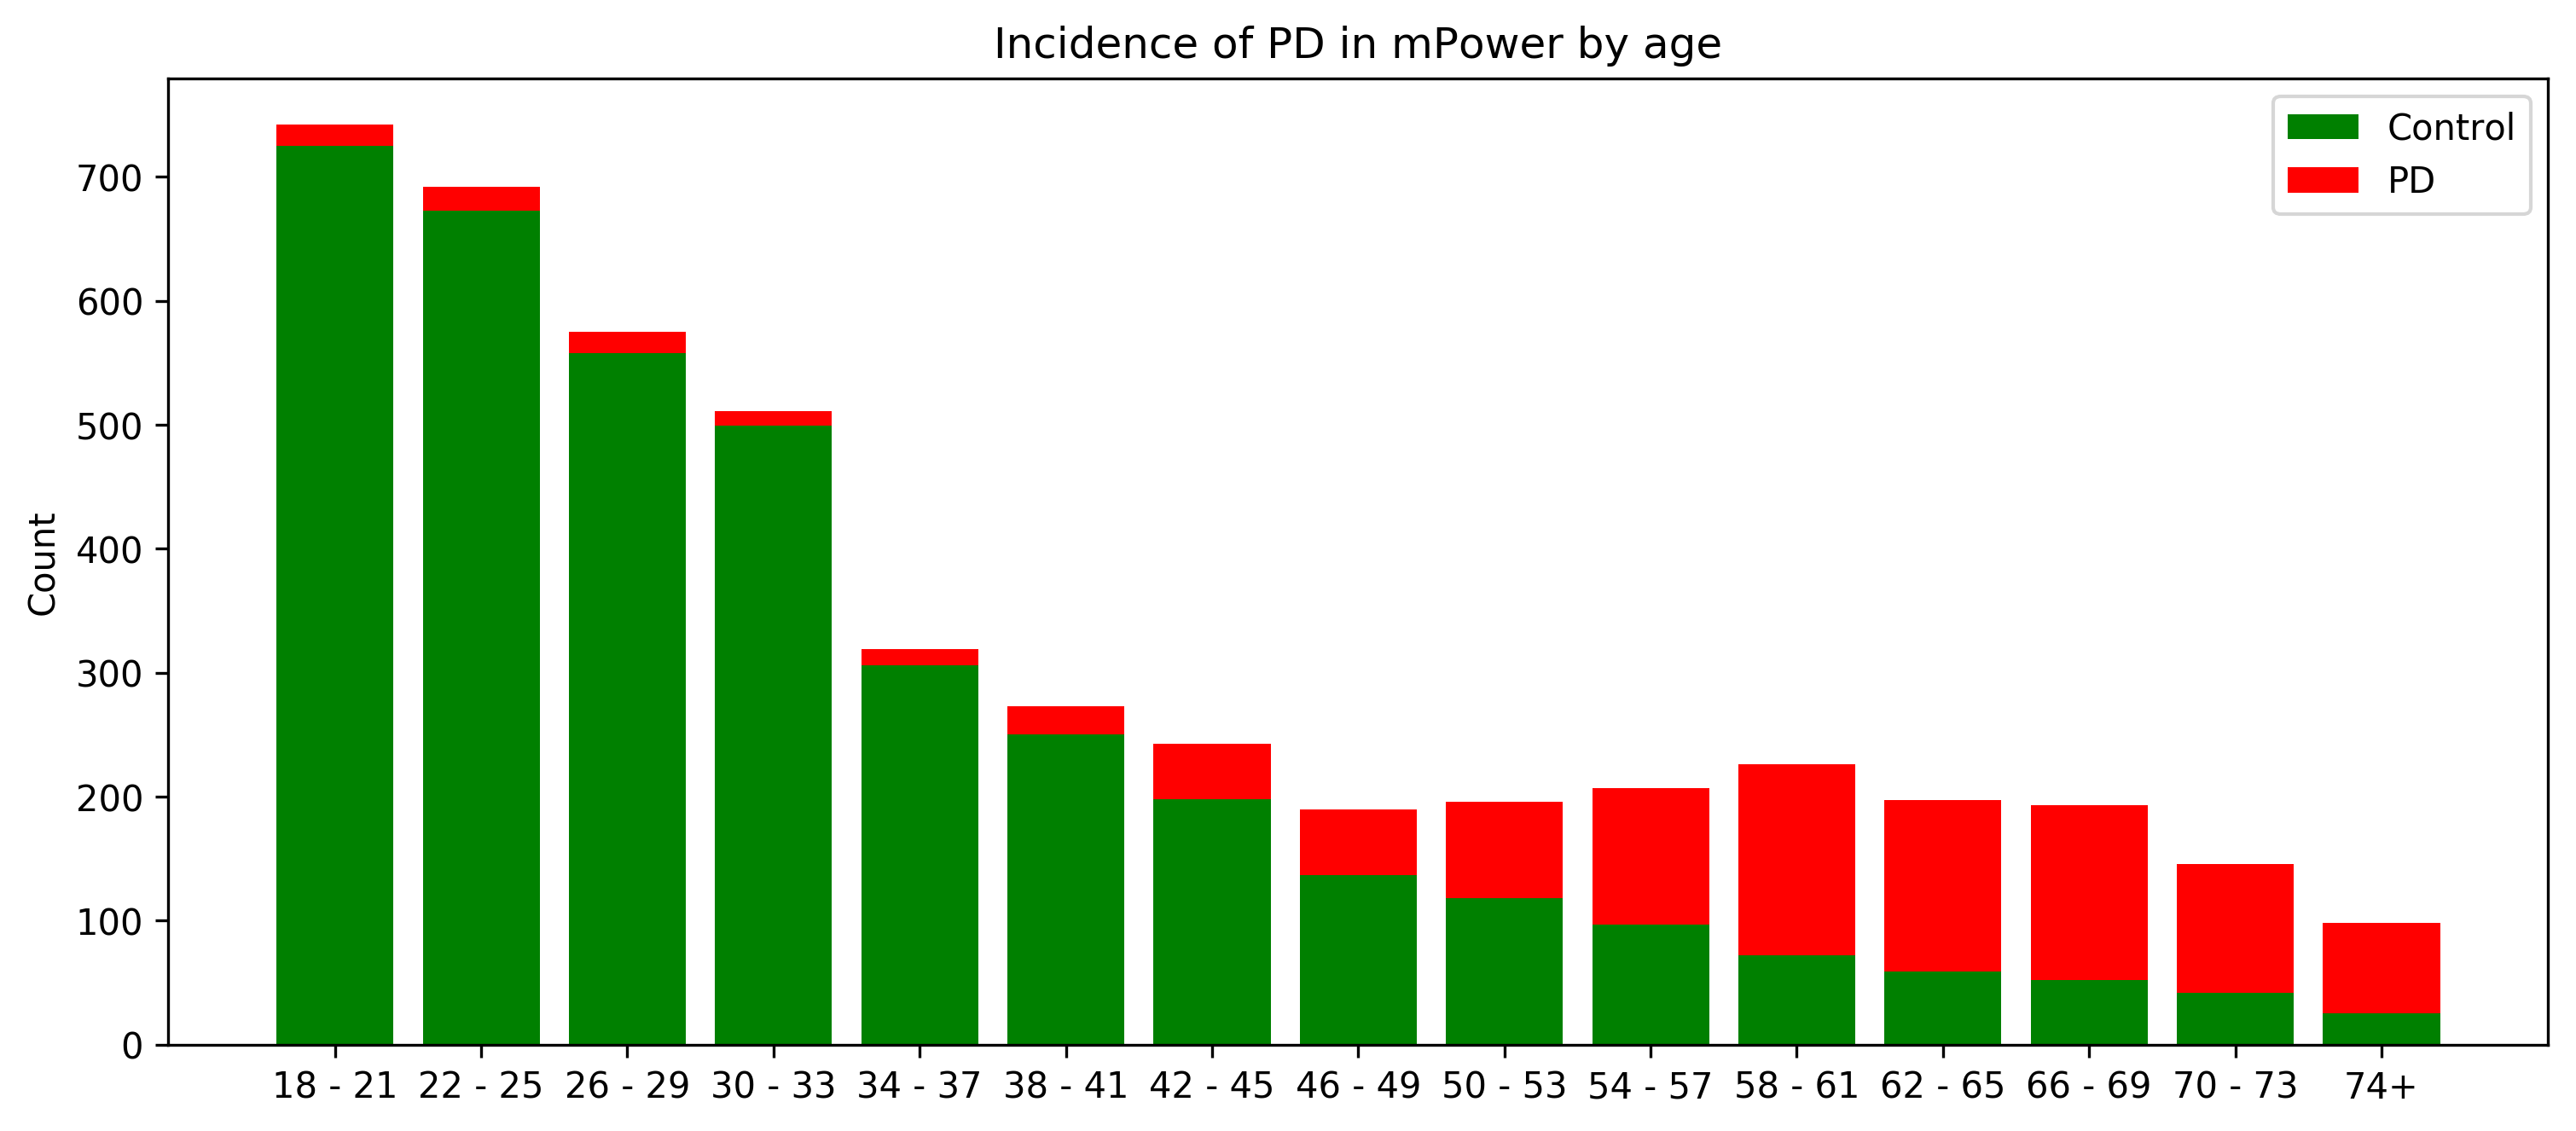
\includegraphics[width=1\linewidth]{mpowerage.png}
\caption{Age is a bias in the mPower dataset as most non-PD participants are young. There are also some cases of rare young-onset PD\protect\footnotemark.}
\end{figure}

%The mPower data study was an experiment in data-collection and was not created with machine learning as a focus. 
The dataset was released late 2015 and has been used in a few studies. The most significant being the recently published Neto~et~al.~\cite{mpowerneto2017analysis}, which provides extensive analysis on the data with respect to medication state and time of the day\footnote{Neto~et~al.~\cite{mpowerneto2017analysis} was published in Jun 29 on arXiv and was not discovered until a late stage literature re-review. Unfortunately techniques introduced in Neto such as detangling medication states and ``time of the day'' effects were not explored due to time limitations.}. A major issue with mPower is that the data is `noisy' --- a common problem in any crowdsourcing project without significant precautions~\cite{crowdsourcing}. 


\subsubsection{Preprocessing and Feature Selection.}
\label{mpowerprocess}
\emph{Vowel phonation} was captured with the single channel iPhone/iPod microphone at 44,100 Hz. Initial investigation showed that a substantial number of participants did not complete the task to an acceptable standard. Excessive levels of environmental noise, hesitation, interruptions or pronouncing vowels other than /aa/ were common. Additionally, the distance between the phone and user varies, with some participants speaking directly into the microphone, creating a large amount of `wind noise'. Preprocessing techniques reduce these interferences exist, but have not been applied to avoid introducing bias to the data~\cite{wang2007speechenhancement, orozco2015voiced,	windnoise}. 

% Although the mPower application prevented access to the voice task when background noise exceeded a certain threshold, this threshold was too lenient. A large number of participants also failed to complete the recording task properly ---

At the time of writing, there were 65,000 phonation samples from 6,000 participants in the mPower dataset (a majority of these from a small number of users). We evaluated 1,600 randomly selected samples for performing the task correctly, rejecting around 25 per cent. Simple metrics such as variance in short time energy and noise prior to recording were used in hand-crafted rules to rank and filter the phonation samples. After filtering, 4,100 users remained, 900 with PD. The highest ranked sample was selected for each of the users\footnote{Optimally, all samples should be used to improve robustness, but available processing power was limited.}. Upon reflection, a valid recording should have been randomly sampled from each participant to avoid the bias of PD participants performing more recordings. Machine learning could optimise this process; however, was avoided due to the possibility of introducing bias to the data. 

%One issue is the varying number of recordings between participants which can be resolved with a participant stratified k-fold CV implementation.

The \emph{walking} task involves the participant putting their phone in the pocket or bag, walking 20 steps then standing still (balancing) for 30 seconds. During this task, accelerometer and gyroscope is continually sampled at $95\pm7$ Hz. Basic features such as the cadence were extracted; however, mPower does not record the parameters necessary (such as leg length) to estimate step length~\cite{diaz2014step}. The characteristics of the signal in-pocket and in-bag would vary significantly, with female users predisposed to having the phone in their bag~\cite{femalephone}. For future data collection projects, phone in hand may be preferable as it introduces fewer variables and does not cause information loss, unlike phone in bag.


%Although in-pocket IMU gait estimation exists~\cite{diaz2014step}, mP. The results of Esser~et~al.~(2011)~\cite{esser2011assessment} suggests that although PD patients on average have a longer cadence, the separation is not clean.

\begin{figure}[!htb]
	\label{mpowerwalking}
	\centering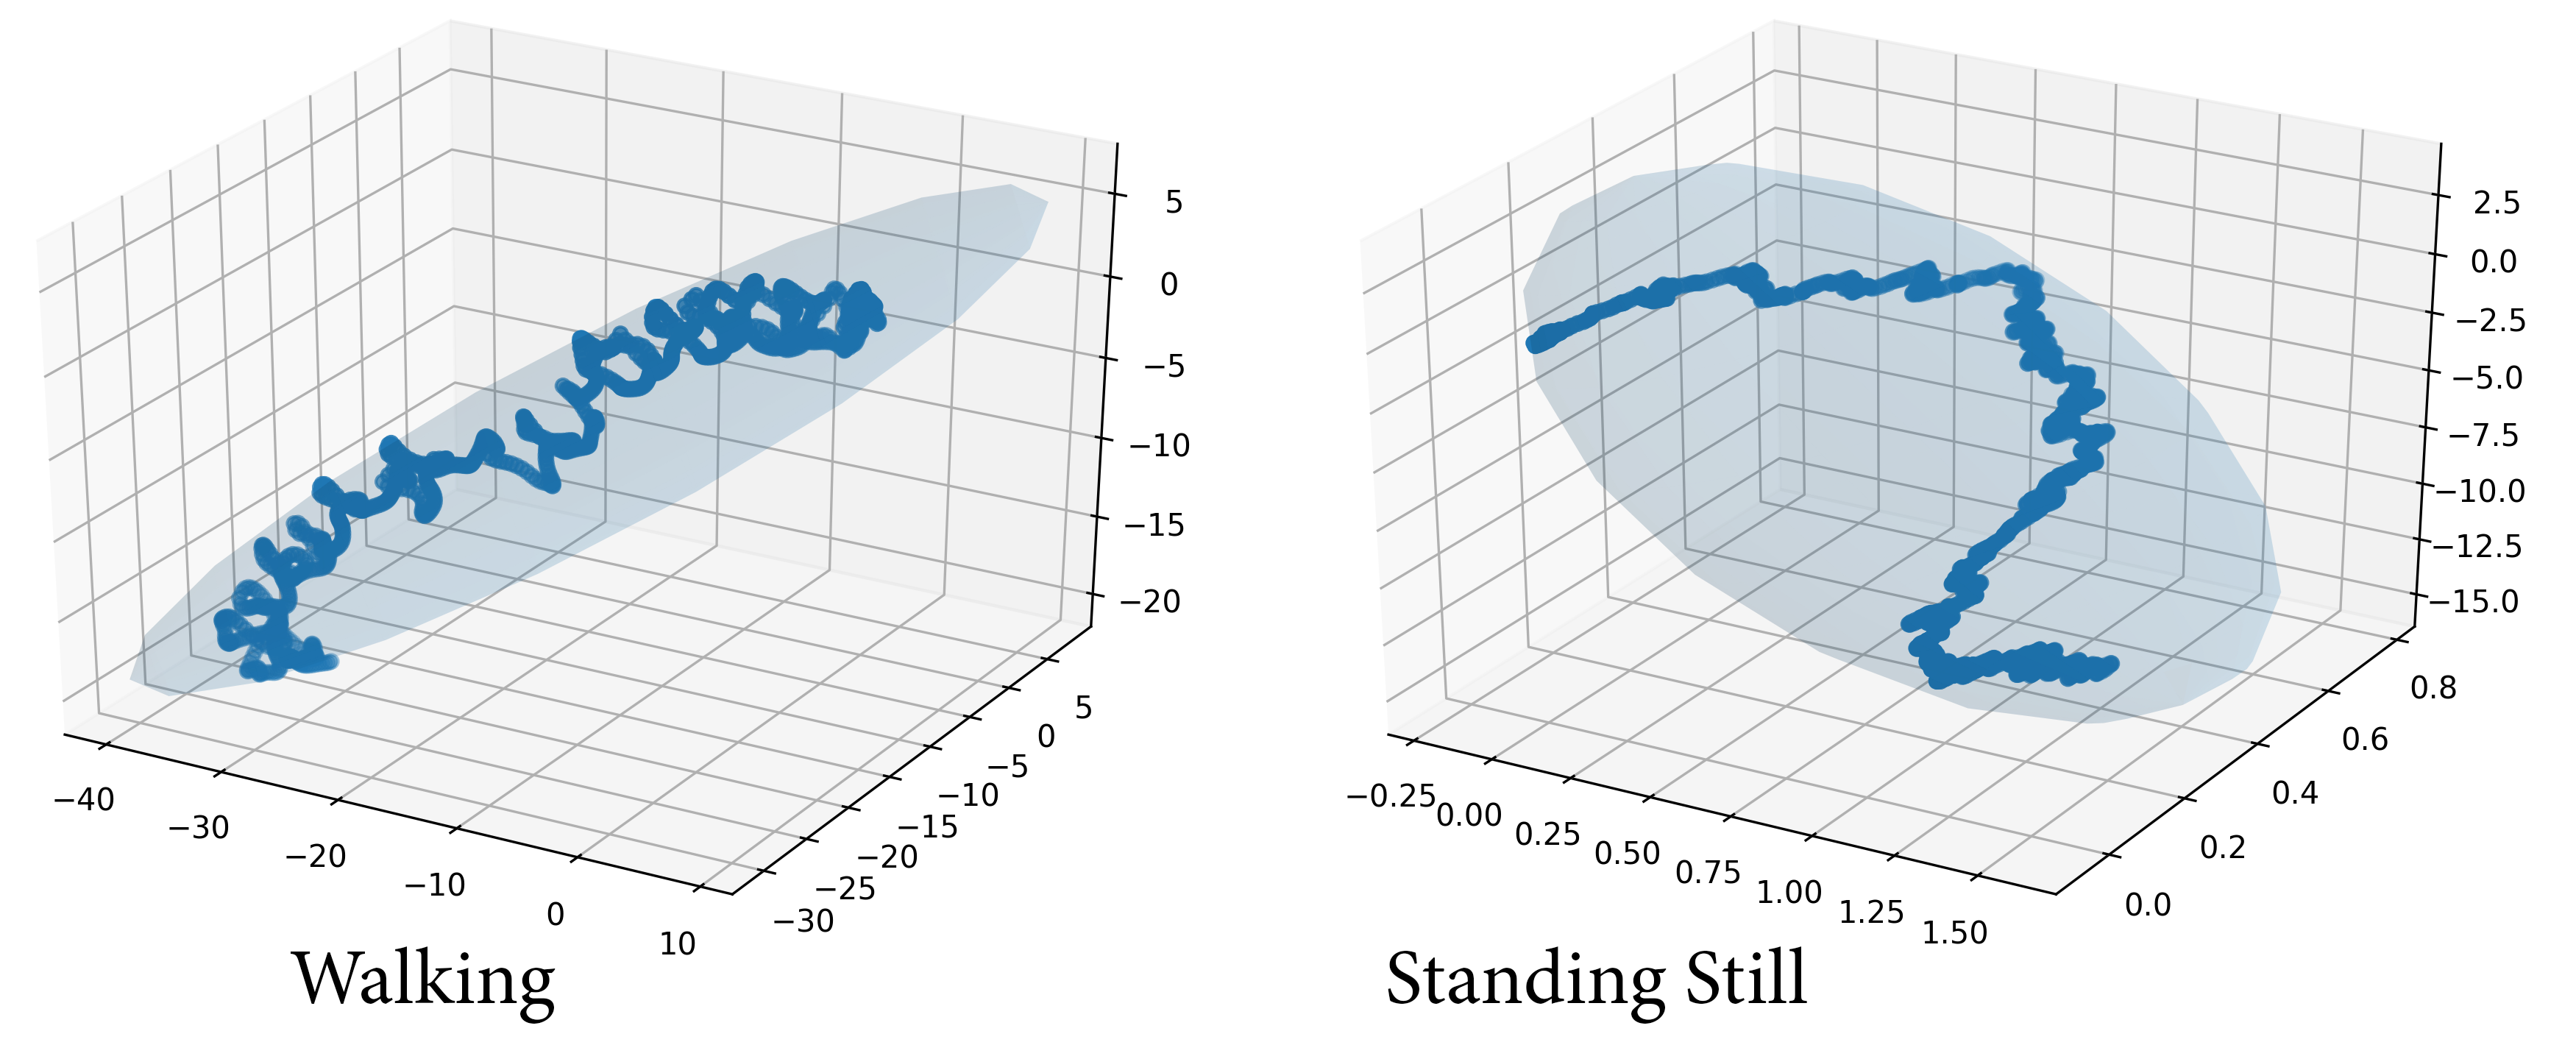
\includegraphics[width=0.9\linewidth]{pathvis3d.png}
	\caption{A visualisation of position from the raw device accelerometer during walking and balancing. The participant appears to be walking on a slope.}
	\vspace{-0.5em}
\end{figure}


As the device is in the user's pocket or bag, data from the gyroscope would be minimally informative. A rotation matrix was computed with the gyroscope data to align the accelerometer's $z$ axis to the direction of gravity. Another rotation was applied to align the average direction of motion with the $x$ axis.

The balancing task aims to simulate the behaviour of standing on a force plate. Unlike force plate experiments, there is no central reference and the subject was not instructed to stand as still as possible. Many participants showed a significant amount of sway which could be consciously preventable. To map the accelerometer to force plate data, a 10\textsuperscript{th} order zero-phase 1hz Butterworth highpass filter was applied (\textit{\hyperref[butterworth]{Figure}} \ref{butterworth}). The highpass filter removed preventable sway at the cost of valuables information below 1hz~\cite{swayspectral}. Additionally, the Anteroposterior and Mediolateral directions of sway were lost with this preprocessing.

\begin{figure}[!htb]
	\centering\centerline{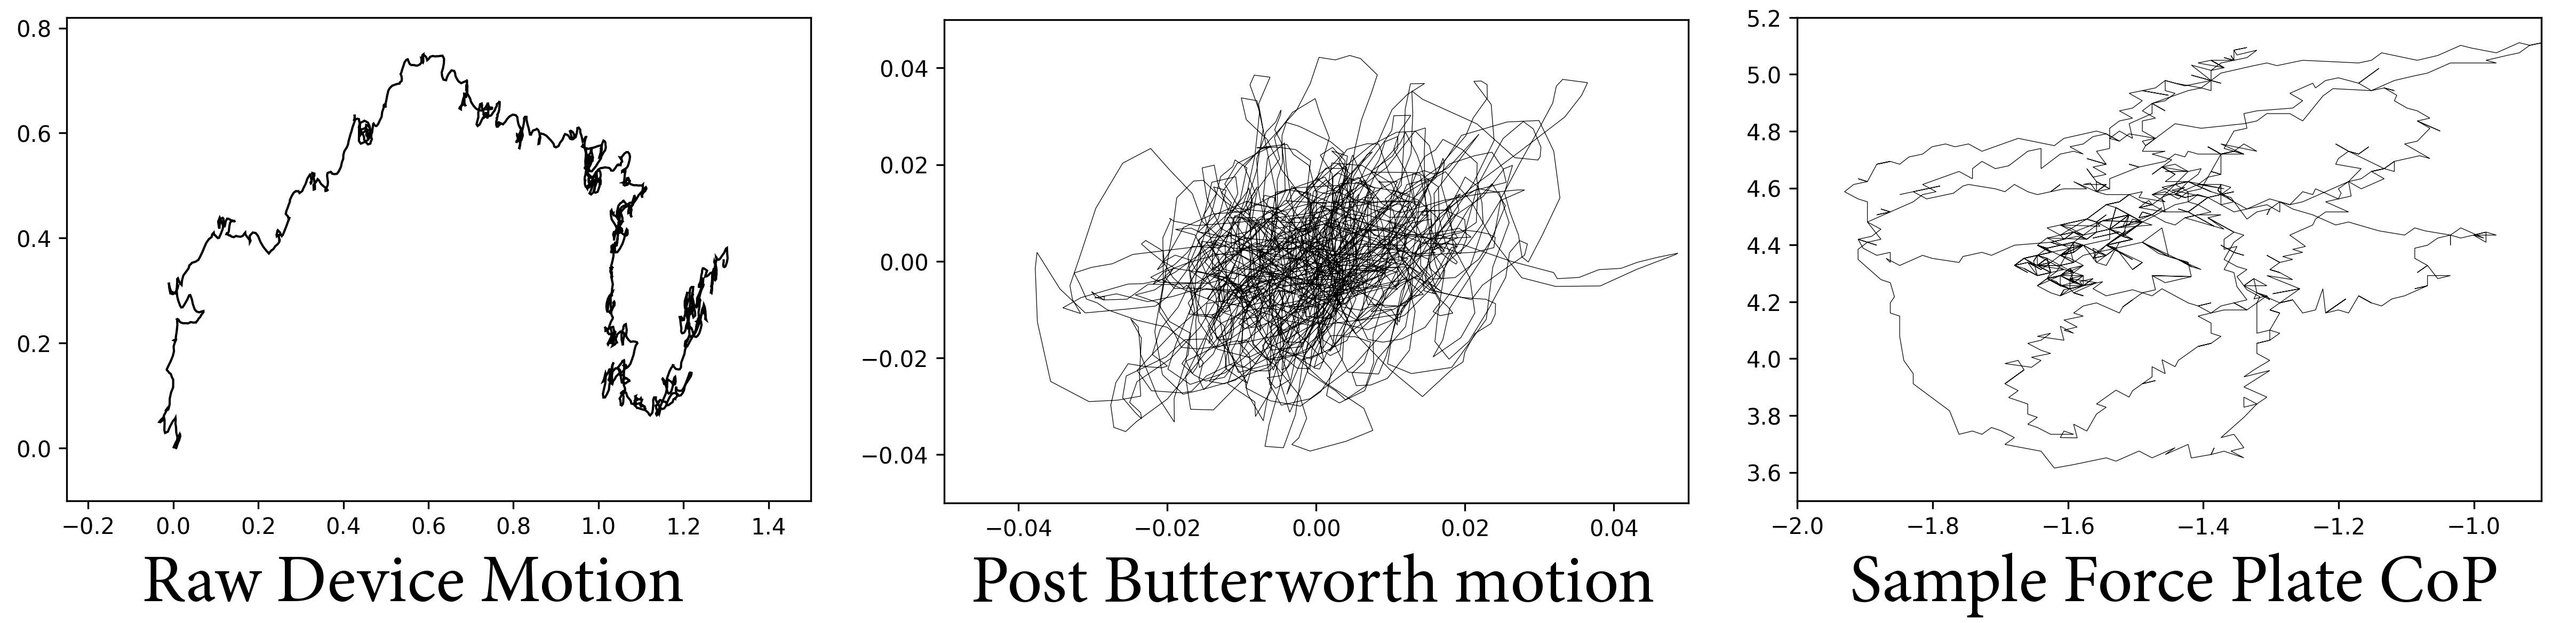
\includegraphics[width=1.15\linewidth]{butterworth.png}}
	\caption{The Butterworth filter results in a device path more similar to the centre of pressure; however, low frequency sway information is lost. Note that the device motion recording is 30 seconds long while the force plate is 10 seconds.}
	\label{butterworth}
	\vspace*{-0.5em}
\end{figure}


A 16 second extract of balance recording between 4s and 20s and the first 10 seconds of the walking task was used for each subject. The choice of these values was solely informed by the nature of the dataset, with the first four seconds of balance data containing significant movement and most recordings of variable length.

Samples which are too short, are corrupted, or have too much variability in recording rate were removed from the set. Approximately 2,300 participants remained with both a valid phonation and movement recording, 600 with PD. The most recent valid sample was selected for each participant, and features specified in \textit{\hyperref[featuresummary]{Section}}~\ref{featuresummary} calculated using the tools and techniques described in \textit{\hyperref[implementation]{Section}}~\ref{implementation}.  Feature engineering was done on both the original and filtered data for the balancing task. Features were computed over the $(x,y)$ and $(x,y,z)$ dimensions for the balancing and walking task respectively.

\begin{highlight}
	One recording of each task per user is selected for machine learning. After preprocessing, the phonation task consists of 4,100 users, 900 with PD, and the movement task consists of 2,300 users, 600 with PD.
\end{highlight}

\newpage
\section{Replicating Past Work}
\label{pastwork}
The work of Tsanas et~al.~\cite{tsanas2012novel} on diagnosis with vowel phonation, and Arora et~al.~\cite{arora2014high} on smartphone accelerometer data was replicated. SVM results are reported as they consistently performed better than random forests and Gaussian processes.

\subsection{Vowel Phonation}
\label{phonationpast}
Tsanas et~al.~\cite{tsanas2012novel} used the National Center for Voice and Speech (NCVS) dataset, which consisted of 33 people with PD, and 10 healthy controls. In total, 263 phonations were recorded in controlled circumstances using a professional grade microphone. HNR, GQ, RPDE, DFA, PPE, GNE, VFER, MFCC and variants of shimmer and jitter were calculated, resulting in a set of 132 features (\textit{\hyperref[featuresummary]{Section}} \ref{featuresummary}).


\begin{figure}[!htb]
	\caption{Cross-validation results of Tsanas~\cite{tsanas2012novel} with a SVM classifier after feature selection. Results reported as mean accuracy $\pm$ std accuracy.}
	\label{tsanasresults}
	\centering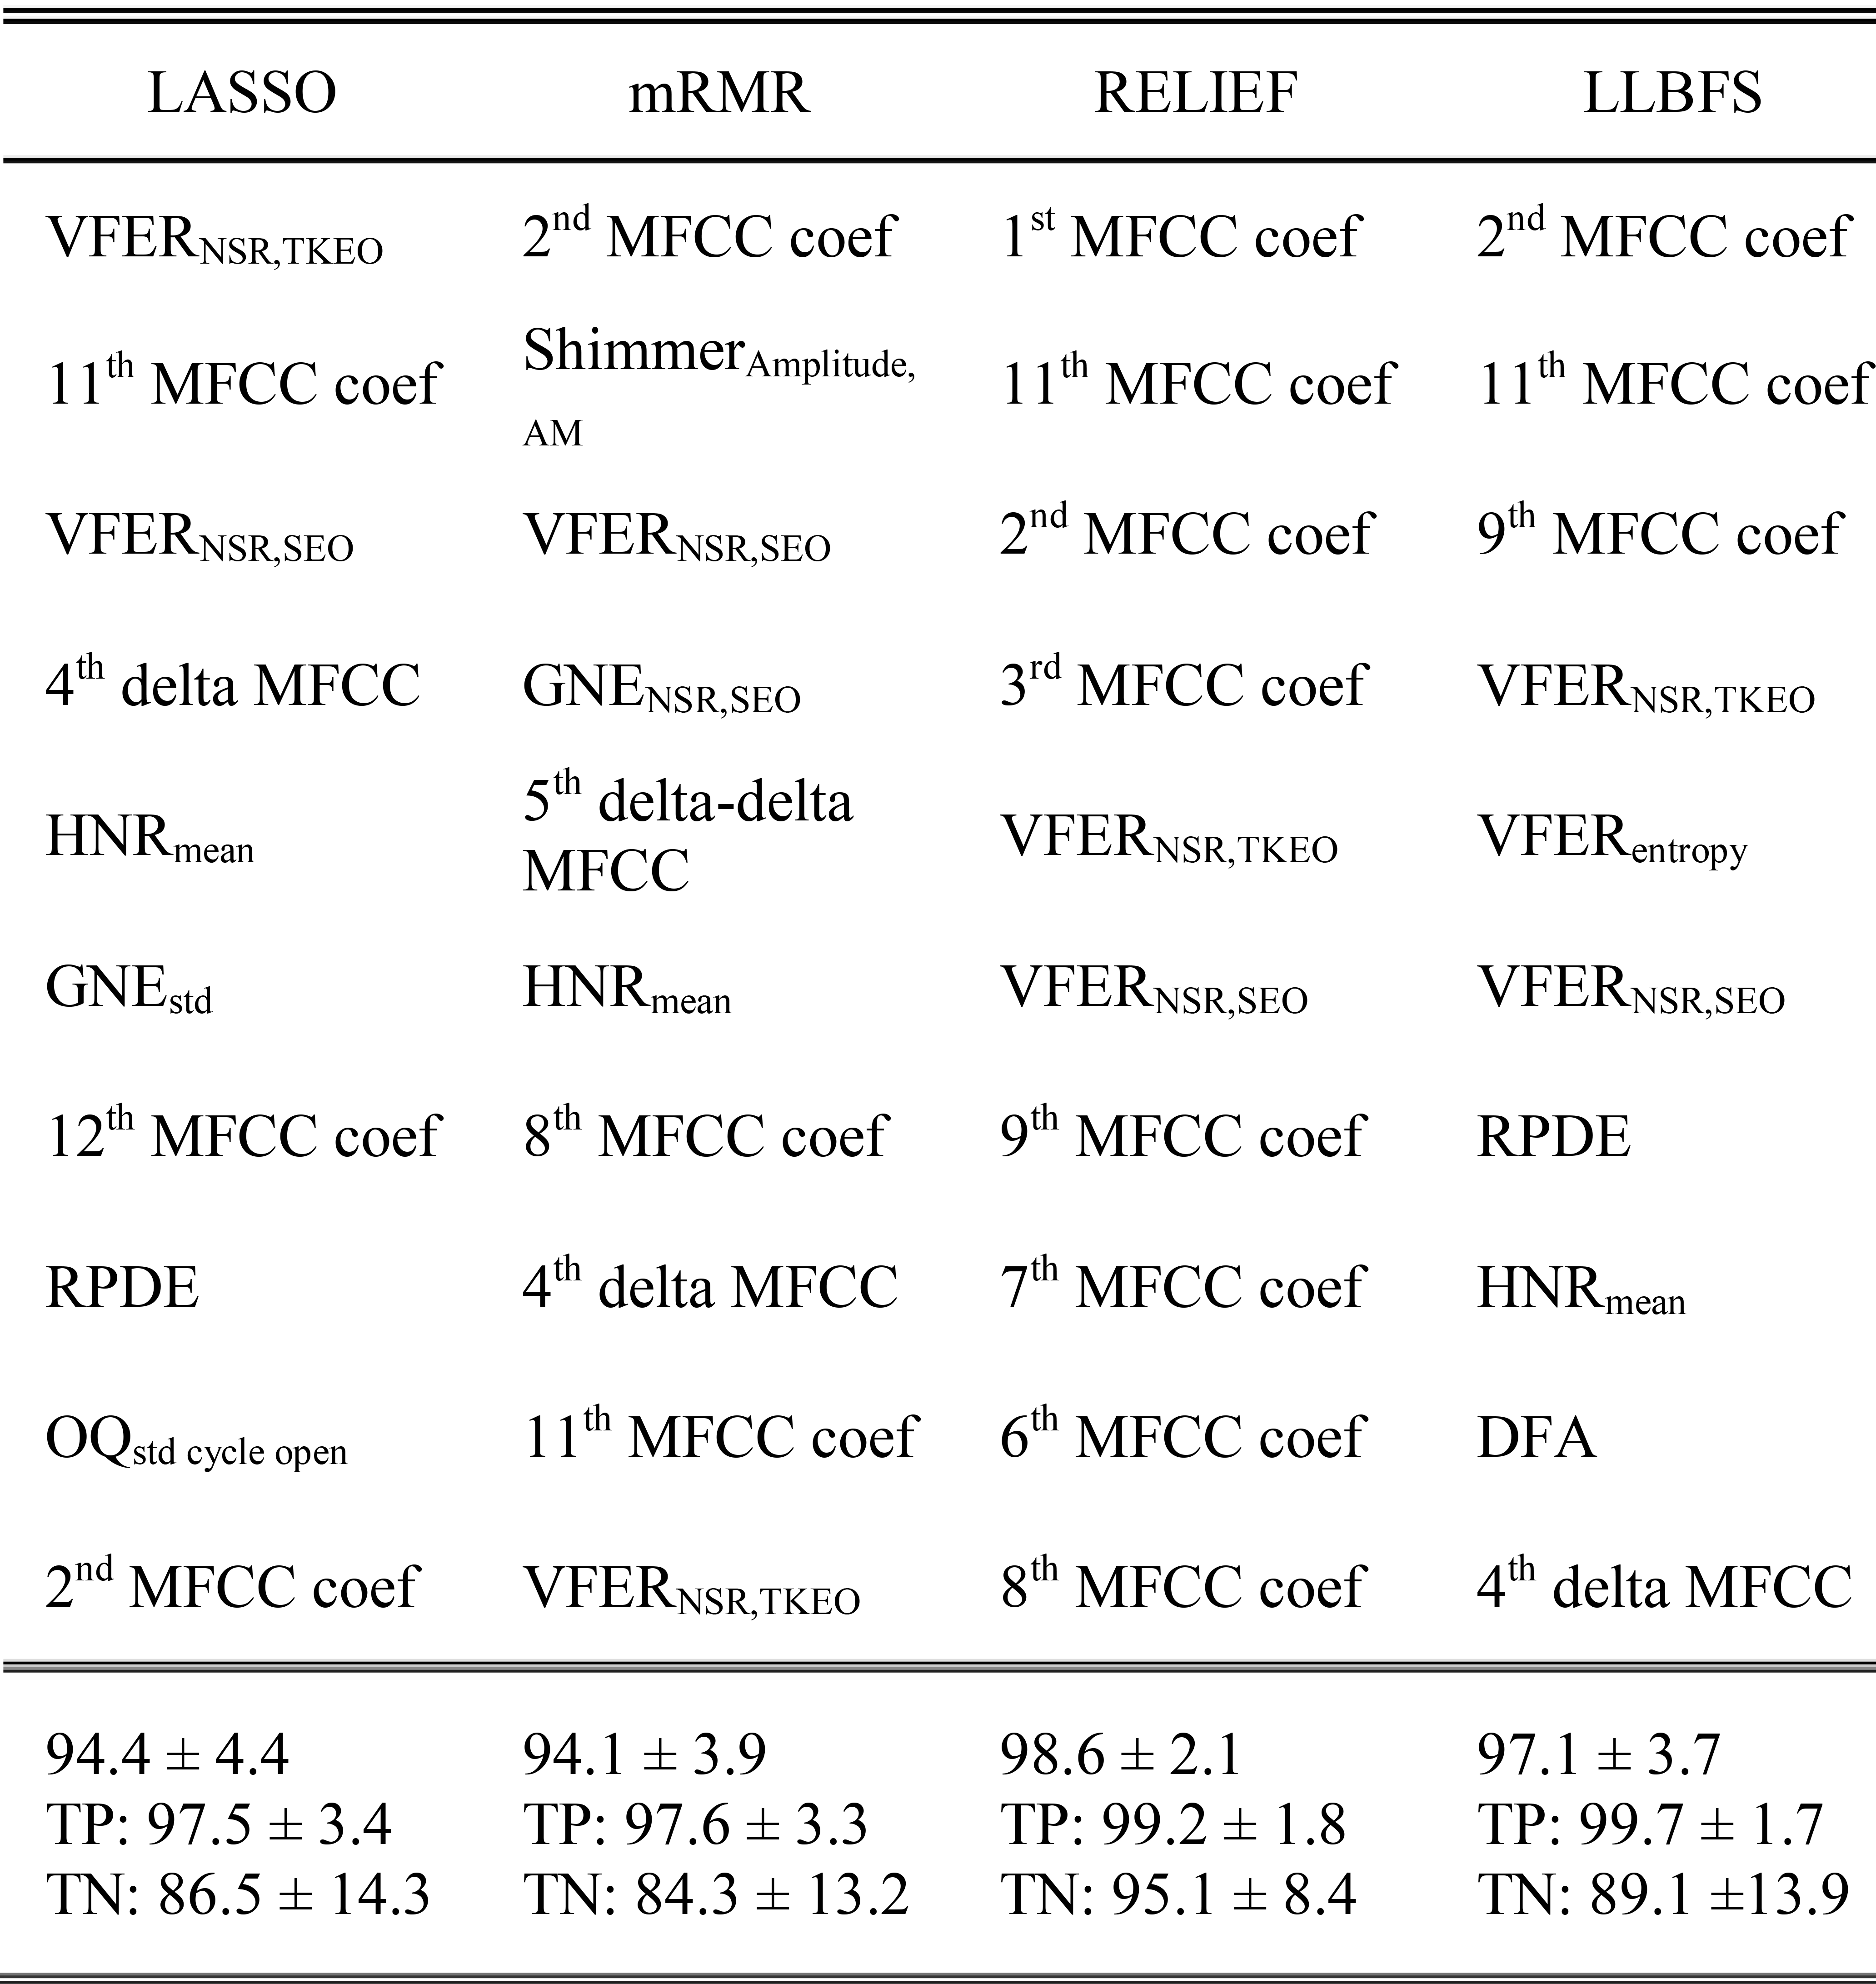
\includegraphics[width=0.75\linewidth]{tsanas.png}
\end{figure}

Features were calculated on the 263 phonations and 100 times repeated 10 fold cross validation used to evaluate models. It is unclear whether Tsanas~et~al. has split the phonations on a per-subject scale --- failure to do so substantially increases risk of overfitting, as phonations from the same subject may appear in both the training and validation set. Random Forests and SVMs were evaluated with hyperparameters selected by gridsearch~\cite{gridsearch}. As data is limited, feature selection with four common algorithms was performed to improve results. This results in the 10 feature subsets depicted in \textit{\hyperref[tsanasresults]{Figure}} \ref{tsanasresults}.


 \begin{highlight}
 	It is unclear whether Tsanas has split the phonations on a per-subject scale and failure to do so presents a substantial risk of overfitting.
 \end{highlight}

We replicated Tsanas on the 3,200PD and 900C phonations selected after preprocessing mPower (see \textit{\hyperref[mpowerprocess]{Section}} \ref{mpowerprocess}). Features were extracted from a 1.5 second window of each audio sample, which is similar to the phonation length used in fundamental frequency estimation datasets~\cite{f0estimation}. Gridsearch was performed to find (near) optimal SVM hyperparameters. The best performing 10 feature subset in Tsanas et~al. (ReliefF) is initially evaluated.

\begin{highlight}[Hyperparameters]
	Unless otherwise specified, search over hyperparameter values were performed for all SVMs. The RBF kernel was always the most effective. Probabilistic output SVMs~\cite{svmprobabilistic} were used for a more accurate AUROC score.
\end{highlight}

Note the NCVS data used in Tsanas et~al. was at a ratio of 33PD:10C, whereas the mPower data is at a ratio of 9PD:32C. We stratified the data by random sampling to simulate NCVS split. On both the NCVS and mPower ratio, the SVM classifier exhibited the false positive paradox --- where the most common class is predicted for all inputs. As evident in \textit{\hyperref[tsanasfsresultsrelieff]{Table}} \ref{tsanasfsresultsrelieff}, the replicated results are significantly poorer than the reported results. 


\begin{table}[!htb]
\caption{Cross validation results of a SVM using Tsanas' 10 feature ReliefF subset (fig \ref{tsanasresults}). Presented as mean $\pm$ standard deviation.}
\label{tsanasfsresultsrelieff}
\centering
\begin{tabular}[t]{c c c}
{\specialcellbold{Equal stratification (50P:50C)}} &&
{\specialcellbold{mPower stratification (9P:32C) }} \\[10pt]
\begin{tabular}{lcl}\hhline{~|*{2}{-}}
	\multicolumn{1}{l|}{}                                 & \multicolumn{1}{l|}{\cellcolor[HTML]{EFEFEF}Pred PD} & \multicolumn{1}{l|}{\cellcolor[HTML]{EFEFEF}Pred C} \\ \hline
	\multicolumn{1}{|l|}{\cellcolor[HTML]{EFEFEF}True PD} & \multicolumn{1}{c|}{$28.2\pm2.6$\%}                          & \multicolumn{1}{c|}{$21.8\pm2.6$\%}                         \\ \hline
	\multicolumn{1}{|l|}{\cellcolor[HTML]{EFEFEF}True C}  & \multicolumn{1}{c|}{$13.5\pm2.4$\%}                          & \multicolumn{1}{c|}{$36.5\pm2.4$\%}                         \\ \hline
	\multicolumn{2}{l}{Accuracy}                                                                                 & $64.7\pm3.0$\%                                              \\
	\multicolumn{2}{l}{Sensitivity}                                                                         & $56.4\pm4.7$\%                                              \\
	\multicolumn{2}{l}{Specificity}                                                                         & $73.0\pm4.4$\%                                               \\
	\multicolumn{2}{l}{AUROC}                                                                         & $69.4\pm4.8$\%                                             
\end{tabular}
& &
\begin{tabular}{lcl}\hhline{~|*{2}{-}}
\multicolumn{1}{l|}{}                                 & \multicolumn{1}{l|}{\cellcolor[HTML]{EFEFEF}Pred PD} & \multicolumn{1}{l|}{\cellcolor[HTML]{EFEFEF}Pred C} \\ \hline
\multicolumn{1}{|l|}{\cellcolor[HTML]{EFEFEF}True PD} & \multicolumn{1}{c|}{$0\pm0$\%}                          & \multicolumn{1}{c|}{$79.2\pm0$\%}                         \\ \hline
\multicolumn{1}{|l|}{\cellcolor[HTML]{EFEFEF}True C} &
\multicolumn{1}{c|}{$0\pm0$\%}                          & \multicolumn{1}{c|}{$21.8\pm0$\%}                         \\ \hline
\multicolumn{2}{l}{Accuracy}                                                                                 & $79.2\pm0$\%                                              \\
\multicolumn{2}{l}{Sensitivity}                                                                         & $0\pm0$\%                                              \\
\multicolumn{2}{l}{Specificity}                                                                         & $100\pm0$\%                                              \\
\multicolumn{2}{l}{AUROC}                                                                         & $72.1\pm4.8$\%                                              
\end{tabular}
\end{tabular}
\vspace{-0.5em}
\end{table}


The ReliefF~\cite{relieff} feature subset in Tsanas~et~al. consisted primarily of MFCC coefficients. MFCC is often the primary feature in speech recognition systems; however, the high and low coefficients are known to be rarely informative in speech recognition~\cite{mfcchistory} --- the ReliefF feature set contains both the 1\textsuperscript{st} and 11\textsuperscript{th} coefficients. The result suggest that high and low coefficients may be informative when used to detect abnormal speech. MFCC are known for being very sensitive to noise and frequency~\cite{mfccrobust,mfccrobust2} and another explanation is the data used in Tsanas~et~al. consisting of controlled recordings, whereas mPower is noisy.

Overfitting is also a possibility. It is ambiguous if Tsanas~et~al. divided phonations of a per-subject level in cross validation. Na\"{i}ve CV may result in  phonations from same individuals appearing in both the training and validation sets. As MFCCs are sensitive to minor changes in frequency~\cite{mfccrobust2}, phonations from different individuals may be easily separable in the MFCC space. This is also supported by the disparity of results between the random forest and SVM classifiers on all features (90.2 per cent vs. 97.7 per cent), as the hyperparameters of the RF classifier were not tuned by cross validation and RF is more robust against overfitting. 


\begin{table}[!htb]
	\caption{Cross validation results of a SVM using all speech features presented in Tsanas~et~al.~\cite{tsanas2012novel}. Decisively outperforms \ref{tsanasfsresultsrelieff} with a Bayes factor of $10^{17}$.}
	\label{tsanasfsresults}
	\centering
	\begin{tabular}[t]{c c c}
		{\specialcellbold{Equal stratification (50P:50C)}} & &
		{\specialcellbold{mPower stratification (9P:32C) }} \\[10pt]
		\begin{tabular}{lcl}\hhline{~|*{2}{-}}
			\multicolumn{1}{l|}{}                                 & \multicolumn{1}{l|}{\cellcolor[HTML]{EFEFEF}Pred PD} & \multicolumn{1}{l|}{\cellcolor[HTML]{EFEFEF}Pred C} \\ \hline
			\multicolumn{1}{|l|}{\cellcolor[HTML]{EFEFEF}True PD} & \multicolumn{1}{c|}{$31.5\pm2.4$\%}                          & \multicolumn{1}{c|}{$18.5\pm2.4$\%}                         \\ \hline
			\multicolumn{1}{|l|}{\cellcolor[HTML]{EFEFEF}True C}  & \multicolumn{1}{c|}{$12.2\pm2.1$\%}                          & \multicolumn{1}{c|}{$37.8\pm2.1$\%}                         \\ \hline
			\multicolumn{2}{l}{Accuracy}                                                                                 & 69.3$\pm$3.3\%                                              \\
			\multicolumn{2}{l}{Sensitivity}                                                                         & 62.9$\pm$4.8\%                                              \\
			\multicolumn{2}{l}{Specificity}                                                                         & 75.6$\pm$4.2\%                                              \\
			\multicolumn{2}{l}{AUROC}                                                                         & $75.7\pm3.4$\%                                                     
		\end{tabular}
		& &
		\begin{tabular}{lcl}\hhline{~|*{2}{-}}
			\multicolumn{1}{l|}{}                                 & \multicolumn{1}{l|}{\cellcolor[HTML]{EFEFEF}Pred PD} & \multicolumn{1}{l|}{\cellcolor[HTML]{EFEFEF}Pred C} \\ \hline
			\multicolumn{1}{|l|}{\cellcolor[HTML]{EFEFEF}True PD} & \multicolumn{1}{c|}{$3.9\pm0.8$\%}                          & \multicolumn{1}{c|}{$16.9\pm0.8$\%}                         \\ \hline
			\multicolumn{1}{|l|}{\cellcolor[HTML]{EFEFEF}True C}  & \multicolumn{1}{c|}{$1.9\pm0.6$\%}                          & \multicolumn{1}{c|}{$77.3\pm0.6$\%}                         \\ \hline
			\multicolumn{2}{l}{Accuracy}                                                                                 & $81.2\pm1.1$\%                                              \\
			\multicolumn{2}{l}{Sensitivity}                                                                         & $18.7\pm4.2$\%                                              \\
			\multicolumn{2}{l}{Specificity}                                                                         & $97.6\pm0.9$\%                                              \\
			\multicolumn{2}{l}{AUROC}                                                                         & $76.7\pm2.9$\%                                                     
		\end{tabular}
	\end{tabular}
\vspace{-0.5em}
\end{table}


In our testing, using all measures presented in Tsanas~et~al. results in improvements over any of the 10 feature subsets presented in \textit{\hyperref[tsanasresults]{Figure}} \ref{tsanasresults}.
\textit{\hyperref[tsanasfsresults]{Table}} \ref{tsanasfsresults} shows the improvement --- it is barely enough to escape the false positive paradox. 

\subsection{Movement}
\label{accelpastwork}
Arora~et~al.~\cite{arora2014high} used smartphone accelerometer data to distinguish 10 healthy and 10 PD participants. Participants were given a LG Optimus S smartphone and instructed to walk 20 steps, turn around, walk 20 steps then stand upright for 30 seconds. The position of the device was not specified --- it is most likely in the participant's pocket. No preprocessing was done to the data, and features engineering included simple statistical and entropy measures, DFA, mean TKEO and the dominant frequency. Arora~et~al. obtained 98 per cent accuracy on with 100 times repeated 10-fold cross validation. Zhan~et~al.~\cite{zhan2016high} extended the feature set and performed a similar experiment on 121 PD and 105 control using additional voice and tapping features; however, only achieved 71 per cent accuracy.

This thesis also coincided with the PD Digital Biomarker DREAM Challenge which involved using accelerometer data to classify PD or predict the UPDRS motor score~\cite{dreamchallengeinfo}. Sage Bionetworks, sponsor of the mPower dataset and a organiser for the challenge released a baseline feature set~\cite{mpowertools} which included all features in Arora~et~al.~\cite{arora2014high}, with additional jerk based measures and the peak of the Lomb-Scargle periodogram~\cite{lombscargle}. The work completed as part of this thesis was submitted to the challenge. The challenge evaluated the trained models on an unreleased portion of the mPower data, validating that our models have not overfit.

%TODO:::::::::::: ADD RESULTS ON DREAM PLSSS

We evaluate both the features in Arora and the DREAM challenge baseline on the mPower accelerometer data. The DREAM baseline is expected to outperform Arora as it is a superset of the features used in Arora. The DREAM features are assumedly an extension of the original code in Arora et al.~\cite{arora2014high} (based on the organiser's affiliations), whereas the Arora feature set is calculated with our own implementation. The models were evaluated on a 50PD:50C stratification of the data to better convey performance.

\begin{table}[!htb]
	\caption{Cross validation results of a SVM on a 50PD:50C stratification of the mPower accelerometer data. Bayes factor of 1.2 --- there is insufficient evidence to conclude the DREAM set outperforms Arora.}
	\label{walkingresults}
	\centering
	\begin{tabular}[t]{c c c}
		{\specialcellbold{Arora Features}} & &
		{\specialcellbold{DREAM baseline features }} \\[10pt]
		\begin{tabular}{lcl}\hhline{~|*{2}{-}}
			\multicolumn{1}{l|}{}                                 & \multicolumn{1}{l|}{\cellcolor[HTML]{EFEFEF}Pred PD} & \multicolumn{1}{l|}{\cellcolor[HTML]{EFEFEF}Pred C} \\ \hline
			\multicolumn{1}{|l|}{\cellcolor[HTML]{EFEFEF}True PD} & \multicolumn{1}{c|}{$30.0\pm3.2$\%}                          & \multicolumn{1}{c|}{$20.0\pm3.2$\%}                         \\ \hline
			\multicolumn{1}{|l|}{\cellcolor[HTML]{EFEFEF}True C}  & \multicolumn{1}{c|}{$17.5\pm2.9$\%}                          & \multicolumn{1}{c|}{$32.5\pm2.9$\%}                         \\ \hline
			
			\\
			
			\multicolumn{2}{l}{Accuracy}                                                                                 & 62.5$\pm$4.2\%                                              \\
			\multicolumn{2}{l}{Sensitivity }                                                                         & 60.0$\pm$6.4\%                                              \\
			\multicolumn{2}{l}{Specificity }                                                                         & 65.0$\pm$5.9\%                                              \\
			\multicolumn{2}{l}{AUROC }                                                                         & $72.1\pm4.8$\%                                                     
		\end{tabular}
		& &
		\begin{tabular}{lcl}\hhline{~|*{2}{-}}
			\multicolumn{1}{l|}{}                                 & \multicolumn{1}{l|}{\cellcolor[HTML]{EFEFEF}Pred PD} & \multicolumn{1}{l|}{\cellcolor[HTML]{EFEFEF}Pred C} \\ \hline
			\multicolumn{1}{|l|}{\cellcolor[HTML]{EFEFEF}True PD} & \multicolumn{1}{c|}{$31.3\pm2.7$\%}                          & \multicolumn{1}{c|}{$18.7\pm2.7$\%}                         \\ \hline
			\multicolumn{1}{|l|}{\cellcolor[HTML]{EFEFEF}True C}  & \multicolumn{1}{c|}{$17.5\pm2.8$\%}                          & \multicolumn{1}{c|}{$32.5\pm2.8$\%}                         \\ \hline
			
			\\
			\multicolumn{2}{l}{Accuracy}                                                                                 & $63.8\pm3.9$\%                                              \\
			\multicolumn{2}{l}{Sensitivity (TP)}                                                                         & $62.6\pm5.4$\%                                              \\
			\multicolumn{2}{l}{Specificity }                                                                         & $65.0\pm5.7$\%                                              \\
			\multicolumn{2}{l}{AUROC (TN)}                                                                         & $72.1\pm4.8$\%                                                     
		\end{tabular}
	\end{tabular}
\end{table}
The results in \textit{\hyperref[walkingresults]{Table}} \ref{walkingresults} fall far from those reported in Arora et al.~\cite{arora2014high}, and mirrors the findings of Zhan et al.~\cite{zhan2016high}. It is clear that performing machine learning in small datasets is a perilous task, with reported results at high risk of overfitting on cross validation. 

\begin{highlight}
	Neither Tsanas' or Arora's results could be replicated on the mPower dataset. 
\end{highlight}


The mediocre performance is not unexpected --- it is unlikely that simple statistical and entropy measures are sufficient to accurately distinguish PD from control. There is a significant amount of noise from variables such as whether the phone was in a pocket or bag and large variance in human gait. This noise is difficult to handle with simple statistical and entropy measures which are sensitive to minor changes in the signal. More advanced signal processing techniques which may be more resistant to the noise will be required.

\newpage
\section{Novel Features for PD Diagnosis}
\label{dynamicalsystems}
The features used in current PD literature are insufficient to accurately perform a diagnosis --- especially given the natural variance of biological signals. EEG signal processing is a field that faces similar issues, with the characteristics of an EEG signal difficult to define. Machine learning with EEG data has evolved to rely primarily on non-linear signal processing techniques. These are detailed in \textit{\hyperref[eegsigproc]{Section}} \ref{eegsigproc} --- the relation of some of these measures to PD symptoms will be summarised below.

Non-linear signal processing involves the estimation more abstract characteristics of a signal. Previously, the nonlinear methods DFA, RPDE and PPE have been applied to phonation~\cite{splittlenonlinear2007,splittledysphonia2009}. DFA and RPDE are measurements quantifying the autocorrelation of a signal, which is expected to be lower in dysphonic phonation due to the variation introduced by turbulent airflow around the incomplete glottal closure. These features may also be applicable to accelerometer data, with the increased tremor and jerking motion from cogwheel rigidity~\cite{cogwheel} resulting in a less stable signal. PPE is a measure of the stability of the fundamental frequency in speech and is less applicable to accelerometer data.

A wider range of non-linear signal processing has been applied on EEG signals. The largest Lyapunov exponent is a measure of the chaos in a system, which is likely higher in dysphonic speech and dyskinetic movement. The fractal dimension relates to the complexity of a signal, and Fisher information and sample entropy measure the unpredictability of a signal. These are likely to be higher in dysphonic speech and dyskinetic movement due to added information from turbulent airflow or tremor and jerking movements. 

\begin{highlight}
The novel features we introduce do not directly relate to human senses and may be more promising at detecting subtle symptoms missed by neurologists.
\end{highlight}

We believe these novel features are more robust measures of symptoms. These features do not directly relate to the information captured by human senses, and may be applicable in detecting symptoms unnoticeable by an expert. We repeated earlier accelerometer and speech experiments on the mPower dataset using the novel features introduced in \textit{\hyperref[eegsigproc]{Section}} \ref{eegsigproc}, with the results recorded in \textit{\hyperref[resultsdynamical]{Table}} \ref{resultsdynamical}. 


\begin{table}[!htb]
	\caption{Cross validation results for a SVM when including the non-linear features. Adding the novel features improves model performance on the accelerometer and phonation data with a Bayes factor of $10^7$ and $10^{12}$ respectively.}
	\label{resultsdynamical}
	\centering\centerline{
	\begin{tabular}[t]{c c c}
		{\specialcellbold{Accelerometer (50PD:50C stratification)}} & 
		{\specialcellbold{Phonation (50P:50C stratification)}} \\[10pt]
		\begin{tabular}{@{}rcccc@{}}
			&  \specialcell{\\DREAM} & \specialcell{Novel \\ Only} & \specialcell{\\Both} \\ \midrule
			Accuracy [\%]    &      $63.8\pm3.9$ &                       $66.0\pm4.0$                                  &        $68.8\pm3.7$\\ \midrule
			Sensitivity [\%] &      $62.6\pm5.4$ &                       $61.8\pm5.7$                                  &     $67.2\pm5.3$\\ \midrule
			Specificity [\%] &      $65.0\pm5.7$ &                       $70.2\pm1.9$                                  &     $70.5\pm5.4$\\ \midrule
			AUROC [\%]         &      $72.1\pm4.8$ &                       $71.3\pm4.5$                                  &     $74.8\pm4.1$\\ \midrule
		\end{tabular}
		&
		\begin{tabular}{@{}cccc@{}}
			\specialcell{\\Tsanas} & \specialcell{Novel \\ Only} & \specialcell{\\Both} \\ \midrule
			$69.3\pm3.3$ &                       $62.9\pm3.5$                                  &       $72.2\pm3.1$ \\ \midrule
			$62.9\pm4.8$ &                       $48.5\pm5.0$                                  &       $69.7\pm4.3$\\ \midrule
			$75.6\pm4.2$ &                       $77.2\pm4.9$                                  &       $74.8\pm4.7$ \\ \midrule
 			$75.7\pm3.4$ &                       $66.6\pm3.9$                                  &       $78.3\pm2.9$\\ \midrule
		\end{tabular}
	\end{tabular}}
\end{table}

The novel features are stronger differentiators of PD than features used in current literature, but not sufficiently to robustly classify PD and control. Bayes Factor analysis shows novel features alone for accelerometer performs better than the DREAM baseline with a $BF=5$. This value is substantial in statistics, but in cross validation implies that the classifiers are succeeding on fairly different examples. Combining both novel features and Tsanas' feature set improves performance greatly on the speech data.

\begin{highlight}[Novel Features]
	The novel features are stronger differentiators of PD; however, there is still more to be desired in terms of performance.
\end{highlight}

\vspace{2em}
\section{Visualising The Features}
\label{visfeature}
In this section, we explore and visualise why models replicated earlier perform well below the reported level in prior works. This disparity is possibly caused by differences in dataset quality --- particularly in ensuring that the task is performed correctly or consistently. It is equally likely that introducing a greater diversity of subjects increases the problem difficulty due to the natural variances in speech and gait. No individual feature could achieve greater than 60\% classification accuracy on an equal stratification of the data. Note that only a fraction of the data is visualised to improve clarity --- more formal analysis of the features is performed in \textit{\hyperref[formalfeatures]{Section}} \ref{formalfeatures}

\begin{highlight}
	No single feature was able to differentiate Parkinson's disease with a greater than 60\% accuracy.
\end{highlight}

\subsection{Speech}
Many dysphonia features rely on precise measurements of the length of each glottal cycle. The SWIPE~\cite{camacho2007swipe} fundamental frequency estimation algorithm was used to obtain these measurements. Most $f_0$ algorithms are sensitive to changes and noise in the signal, and are not yet suitable to handle the noisy mPower data. Issues with $f_0$ extraction would invalidate the measurements of a number of features. A simple investigation shows that the standard deviation of $f_0$ (\textit{\hyperref[stdevf0]{Figure}} \ref{stdevf0}) exceeds 10Hz for 347 subjects, a value that indicates a failure of the algorithm or a poorly executed recording.

\begin{figure}[!htb]
	\centering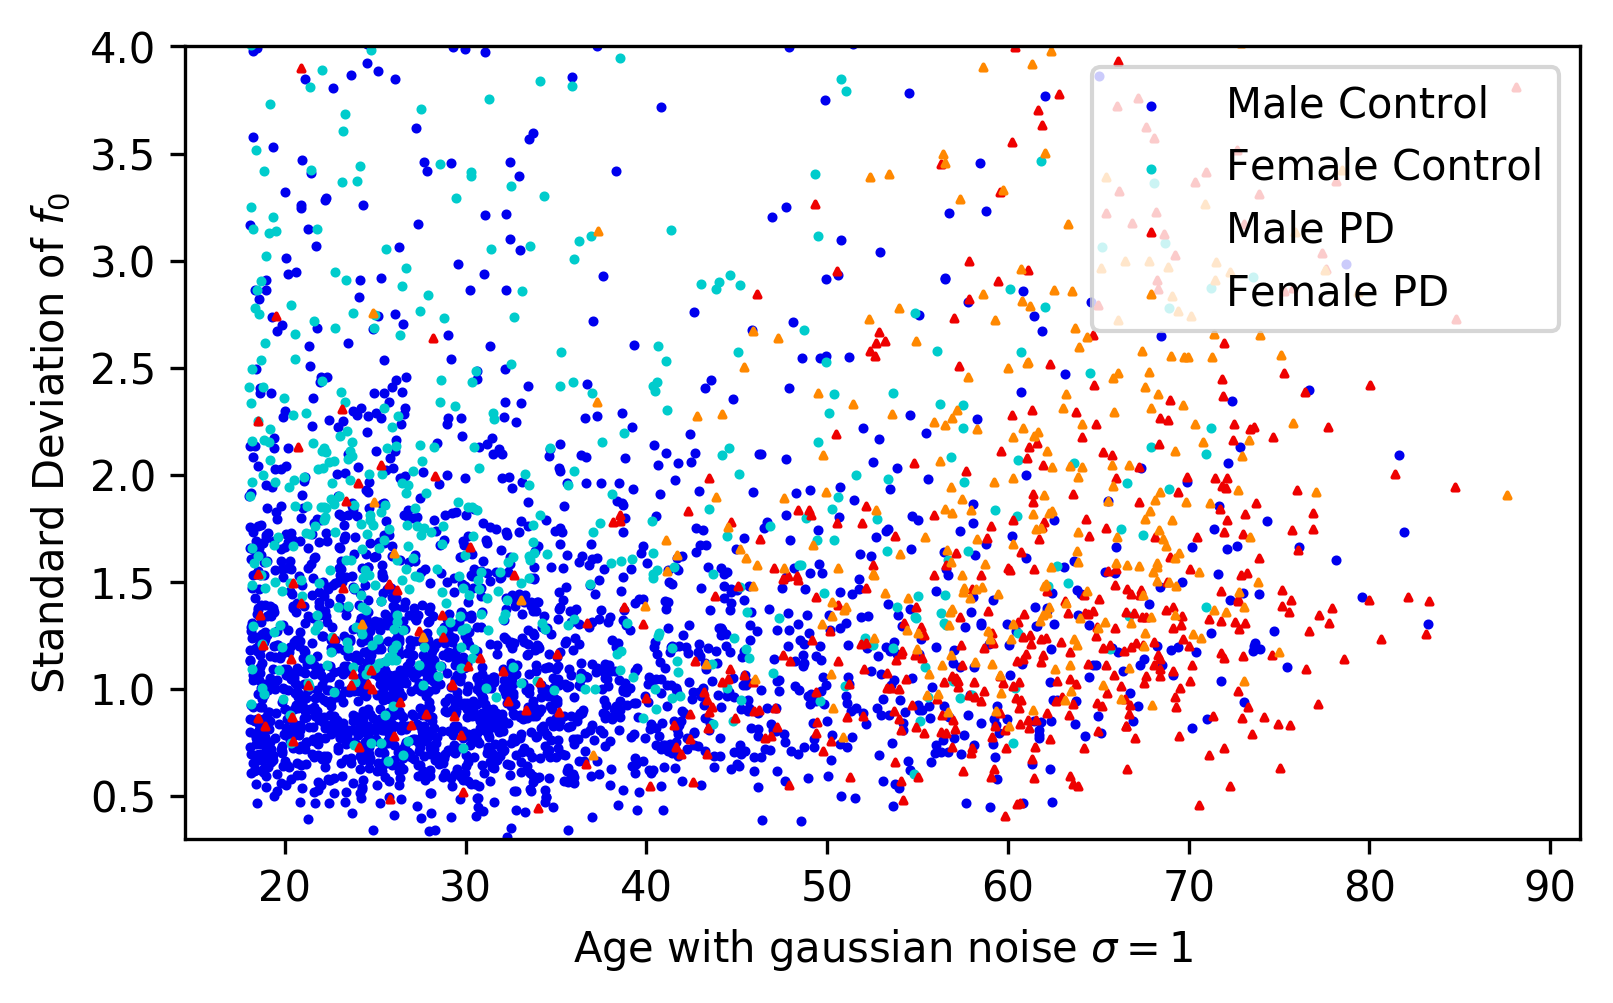
\includegraphics[width=0.67\linewidth]{f0stdev.png}
	\caption{Standard Deviation of the fundamental frequency during phonation. Females and older individuals exhibit notably higher variations in $f_0$, whereas the distinction between age matched PD and control participants is less clear.}
	\label{stdevf0}
\end{figure}

\begin{figure}[!htb]
	\centering\centerline{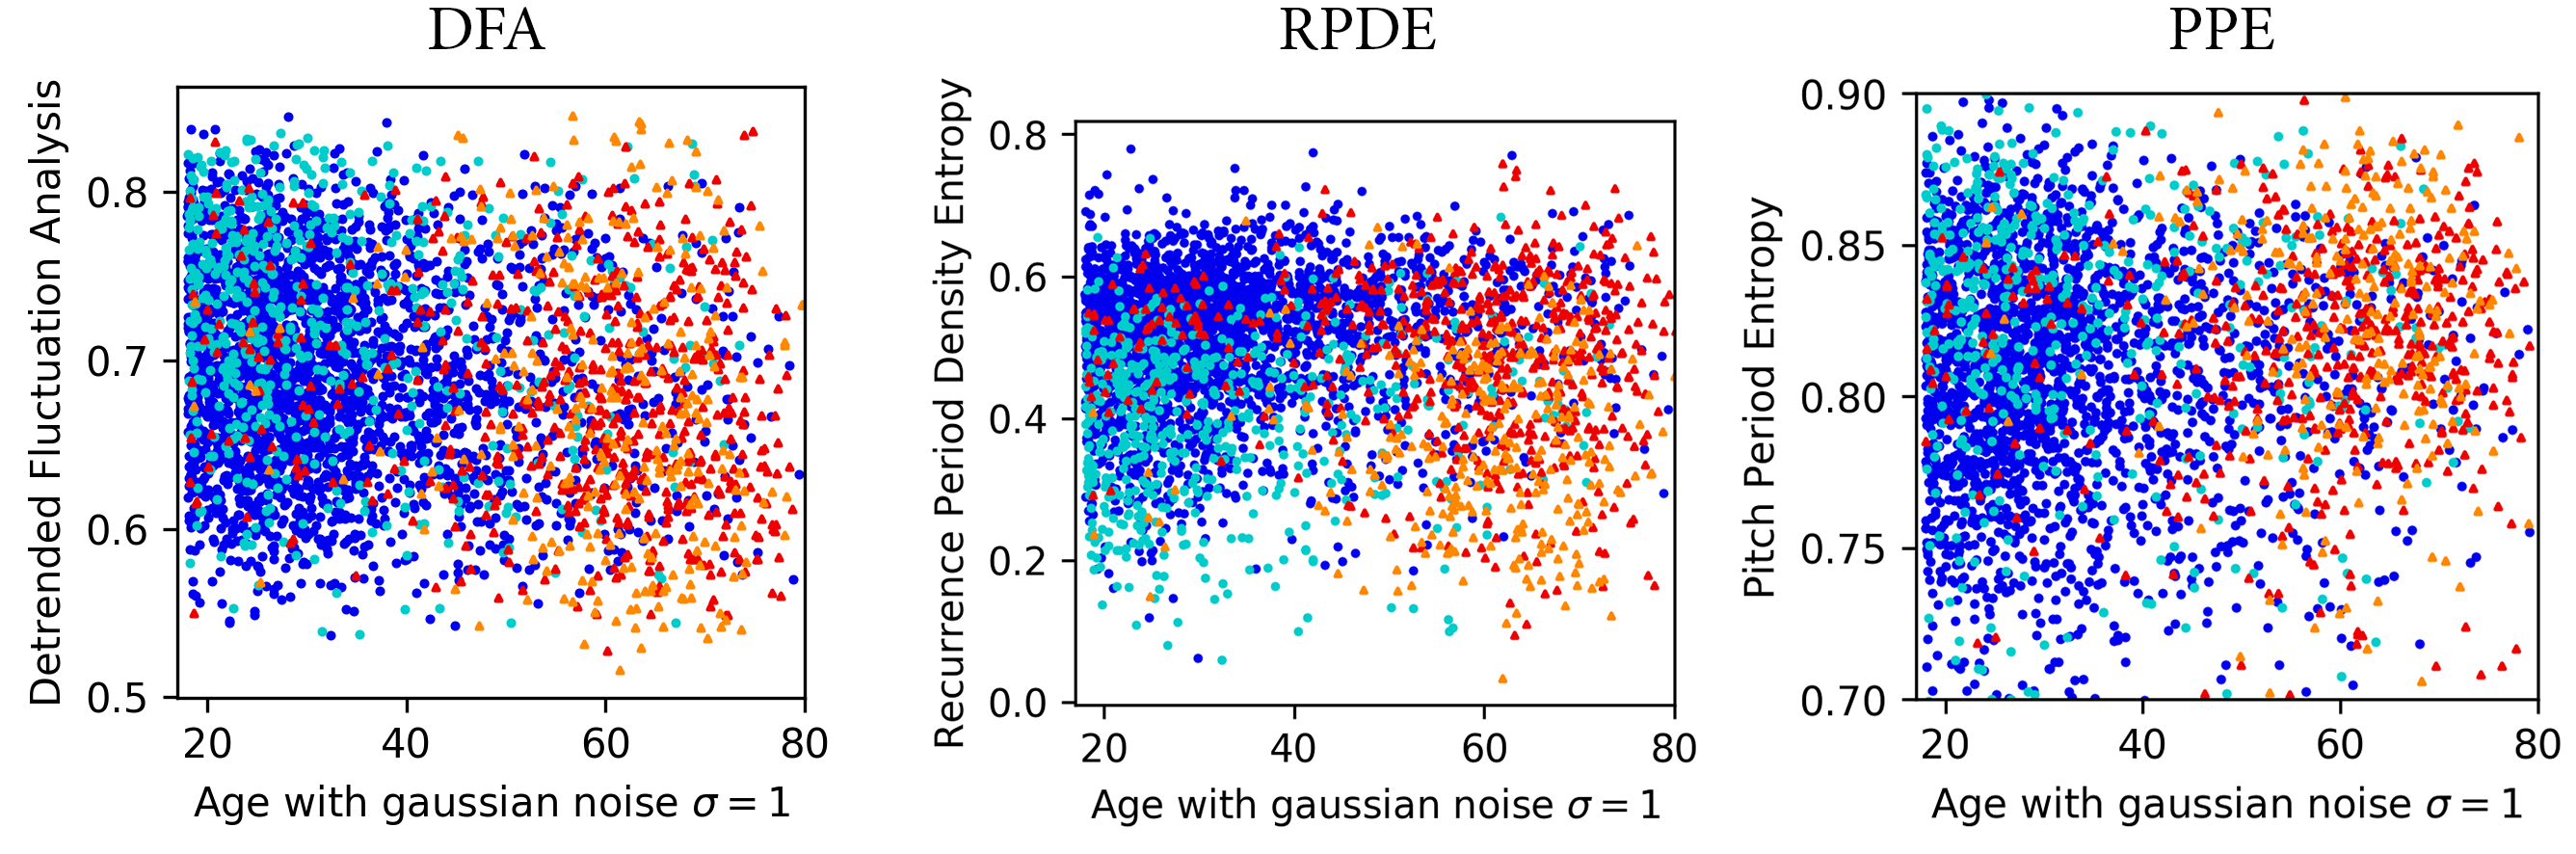
\includegraphics[width=0.82\linewidth]{dfapperpde.png}}
	\caption{PD subjects exhibit a lower DFA and RPDE, and a higher PPE. However, these features are hardly separable. A combination of DFA and RPDE significantly enhances the separability of female participants with PD. See \textit{\hyperref[stdevf0]{Figure}} \ref{stdevf0} for legend.}
	\label{dfapperpde}
	\vspace{-1.5em}
\end{figure}


Little~et~al.~\cite{splittlenonlinear2007,splittledysphonia2009} introduced three measures to distinguish dysphonia --- DFA, RPDE and PPE. DFA and RPDE are measures of the autocorrelation of a signal. As evident in \textit{\hyperref[dfapperpde]{Figure}} \ref{dfapperpde}, people with PD exhibited a lower autocorrelation than age matched control subjects, indicative of a more chaotic and variable speech signal. People with PD also show an increase in PPE to age matched control, which is evidence of fluctuations in pitch above healthy speech production. However, distinguishing dysphonic speech is not easy due to the natural variance in speech production.


\begin{figure}[!htb]
	\centering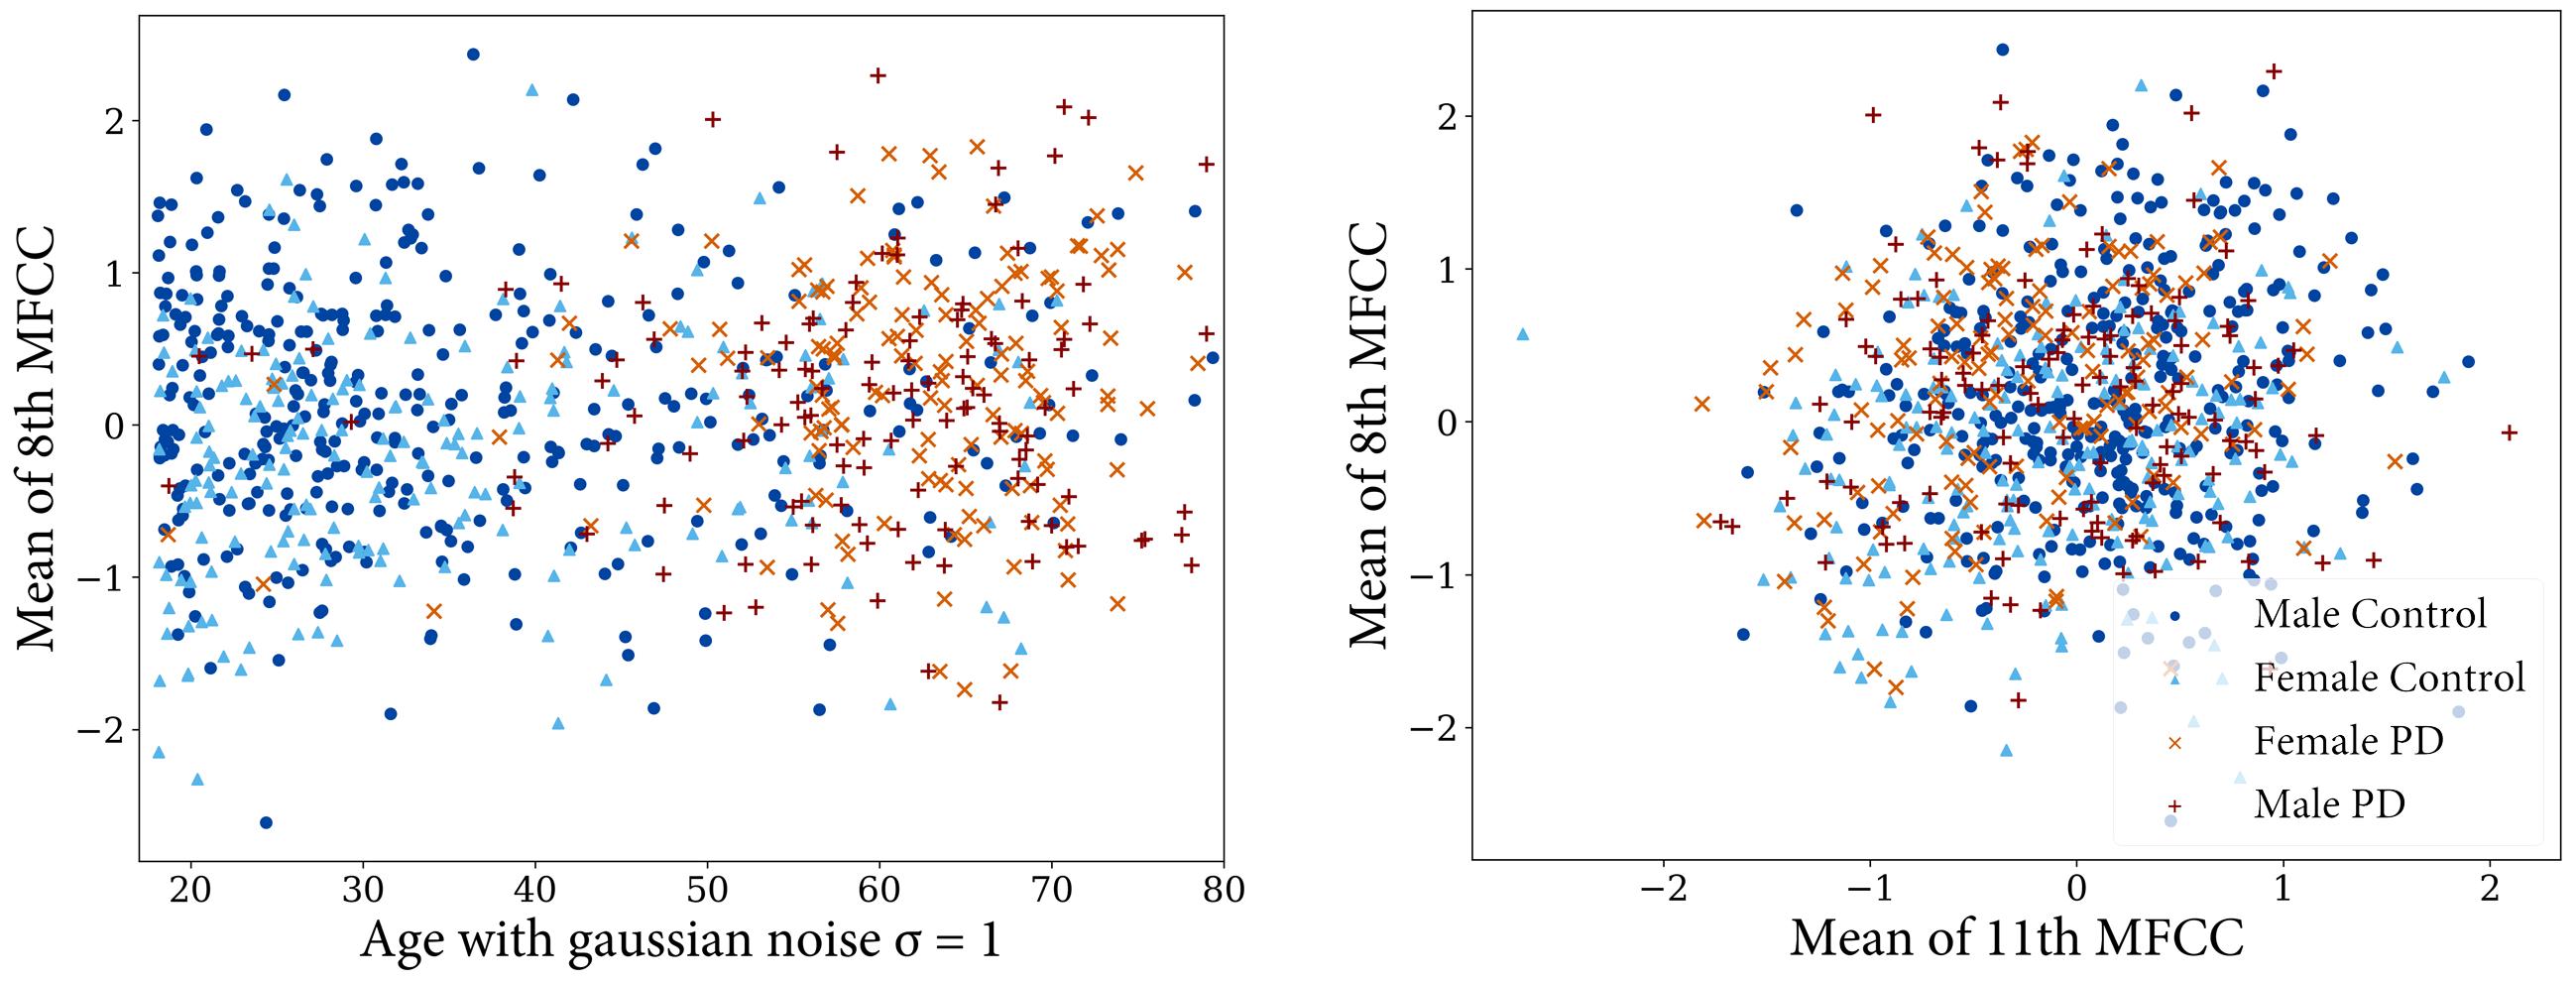
\includegraphics[width=1\linewidth]{mfcc_feat.png}
	\caption{Unlike Benba~\cite{benba2014mfcc}, the 8\textsuperscript{th} MFCC coefficient is not a notable for distinguishing dysphonia. A combination of multiple MFCC adds marginally more information. }
	\label{mfcc_feat}
	\vspace{-0.5em}
\end{figure}

Benba et~al.~\cite{benba2014mfcc} distinguished PD with a 82 per cent success rate primarily with MFCC, which are also present in most of the feature subsets derived by Tsanas et~al.~\cite{tsanas2012novel}. Being the primary feature in most speech recognition systems, it is not surprising MFCC are strong features in detecting dysphonia. However, \textit{\hyperref[mfcc_feat]{Figure}} \ref{mfcc_feat} suggests that there is a very minimal correlation between MFCC and PD. The MFCC are very sensitive to changes in the signal, and more advanced measures than the mean and standard deviation may be required to fully utilise them. An example is using a LSTM neural network, which is common in speech recognition~\cite{convlstm}.




\begin{figure}[!htb]
	\centering
	\centerline{
		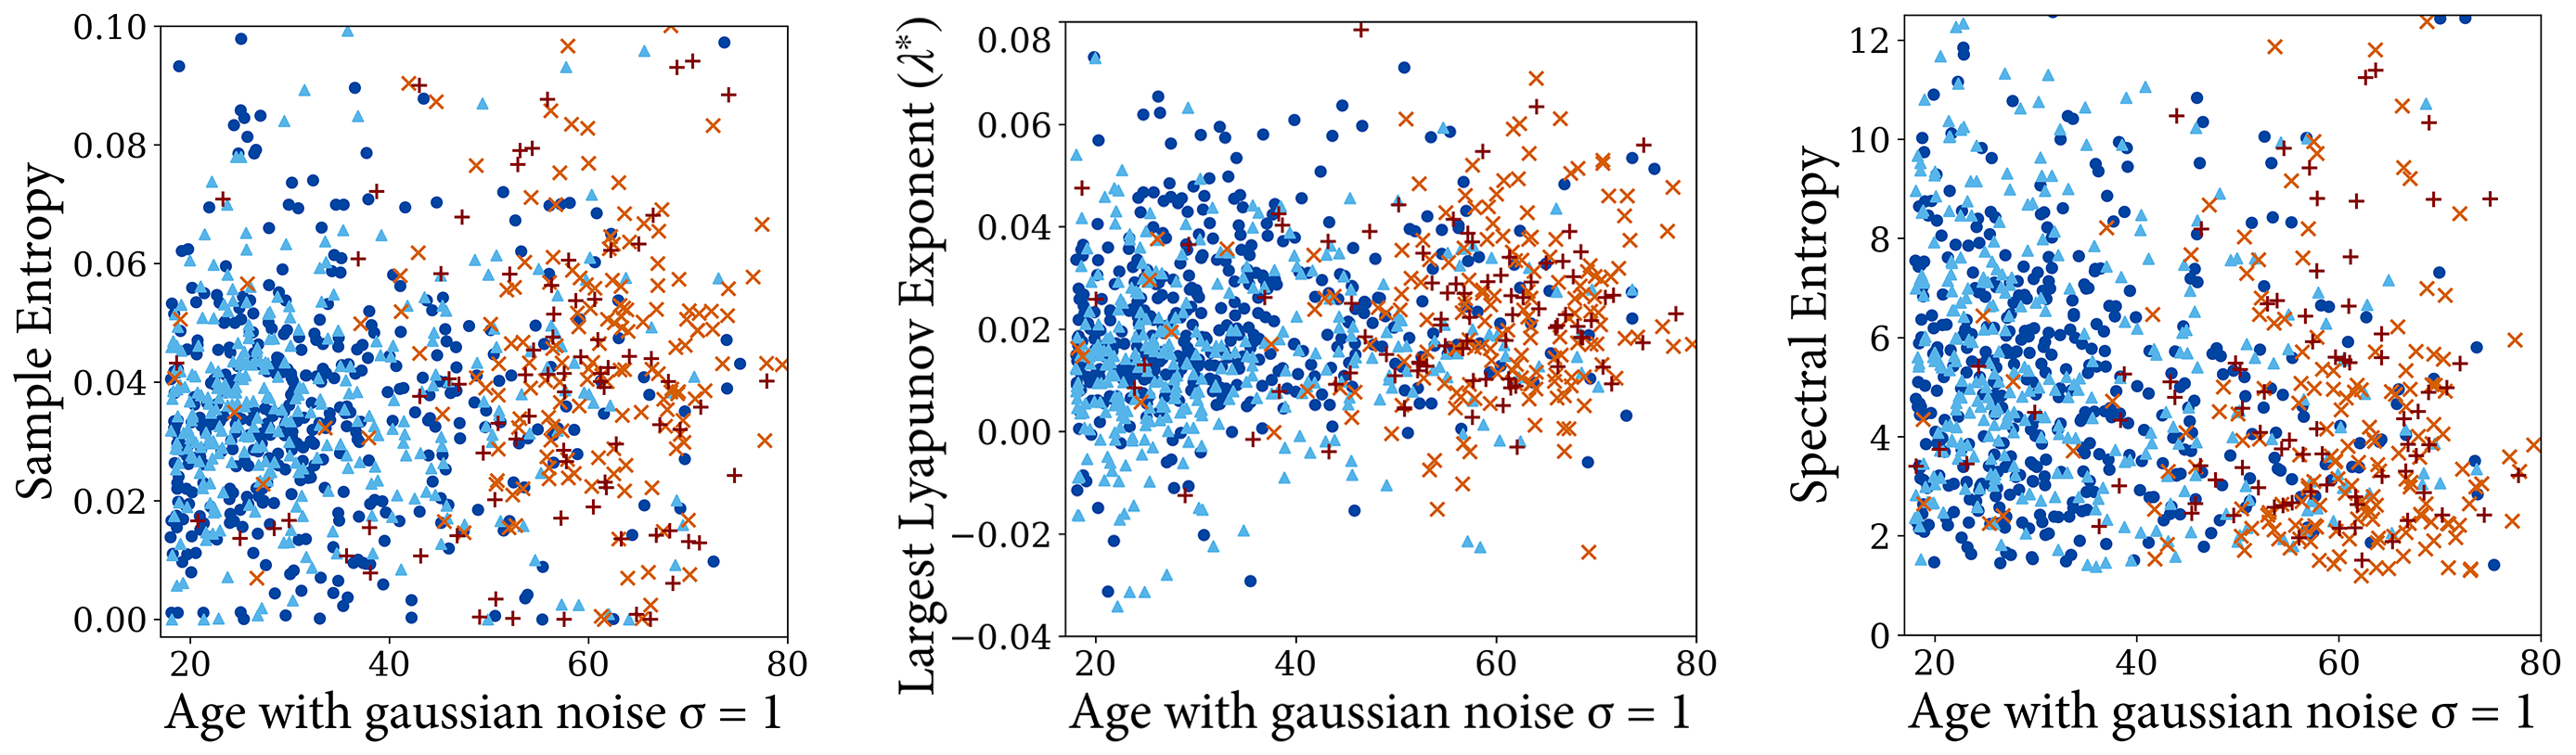
\includegraphics[width=1.15\linewidth]{speech_dynamic.png}
	}
	\caption{A visualisation of some nonlinear speech features. Sample entropy and $\lambda^*$ (measures of unpredictability) are higher in subjects with PD, whereas spectral entropy is lower. See \textit{\hyperref[mfcc_feat]{Figure}} \ref{mfcc_feat} for legend.}
	\vspace{-0.5em}
	\label{speechdynamic}
\end{figure}

The novel features introduced in \textit{\hyperref[eegsigproc]{Section}} \ref{eegsigproc} are strong differentiators of PD. As expected, the sample entropy and largest Lyapunov exponent ($\lambda^*$) are greater in participants with Parkinson's Disease, indicative of a more chaotic/unpredictable signal. The lower spectral entropy is indicative of a more even distribution of the frequencies, which can be visualised in the `blurry' nature of the spectrogram in \textit{\hyperref[spectrogram]{Figure} \ref{spectrogram}}. 




The largest Lyapunov exponent was mostly positive during the phonation of /aa/, with female participants with PD in particular exhibiting a greater $\lambda^*$. This is also a significant result for literature analysing the non-linearity of speech with $\lambda^*$ as it was conducted on a very large dataset. This provides evidence for results indicating a slightly positive $\lambda^*$ in vowel phonation~\cite{kokkinos2005nonlinearlyapunov, lyapunovpositive} rather than close to zero~\cite{banbrook1999speechlyapunov, lyapunovzero}.

\subsection{Movement}
Understanding the features extracted for the movement data is a trickier task. Like speech, a significant amount of variance will exist based on physical factors (such as leg length) and environmental factors (such as depth/tightness of pocket). The mPower application asked the user to place their phone in either their pocket or bag, and there likely exists a tendency for females to complete the activity with their phone in a bag~\cite{femalephone}. This choice of experimental design may limit machine learning potential, as information will be lost from the padding and pendulum motion of shoulder bags and padding. A better setup would be to ask participants to hold the device in their hand --- although additional variability is introduced, this could be filtered whereas lost information cannot be recovered.

Accelerometer signals contain three dimensions of data ($x,y,z$). Rotations have been performed such that the $z$ axis is aligned with gravity, and the average direction of the walk is aligned with the $x$ axis. Features are visualised as the mean value over all dimensions.

\begin{figure}[!htb]
	\centering
	\begin{subfigure}{.5\textwidth}
		\centering
		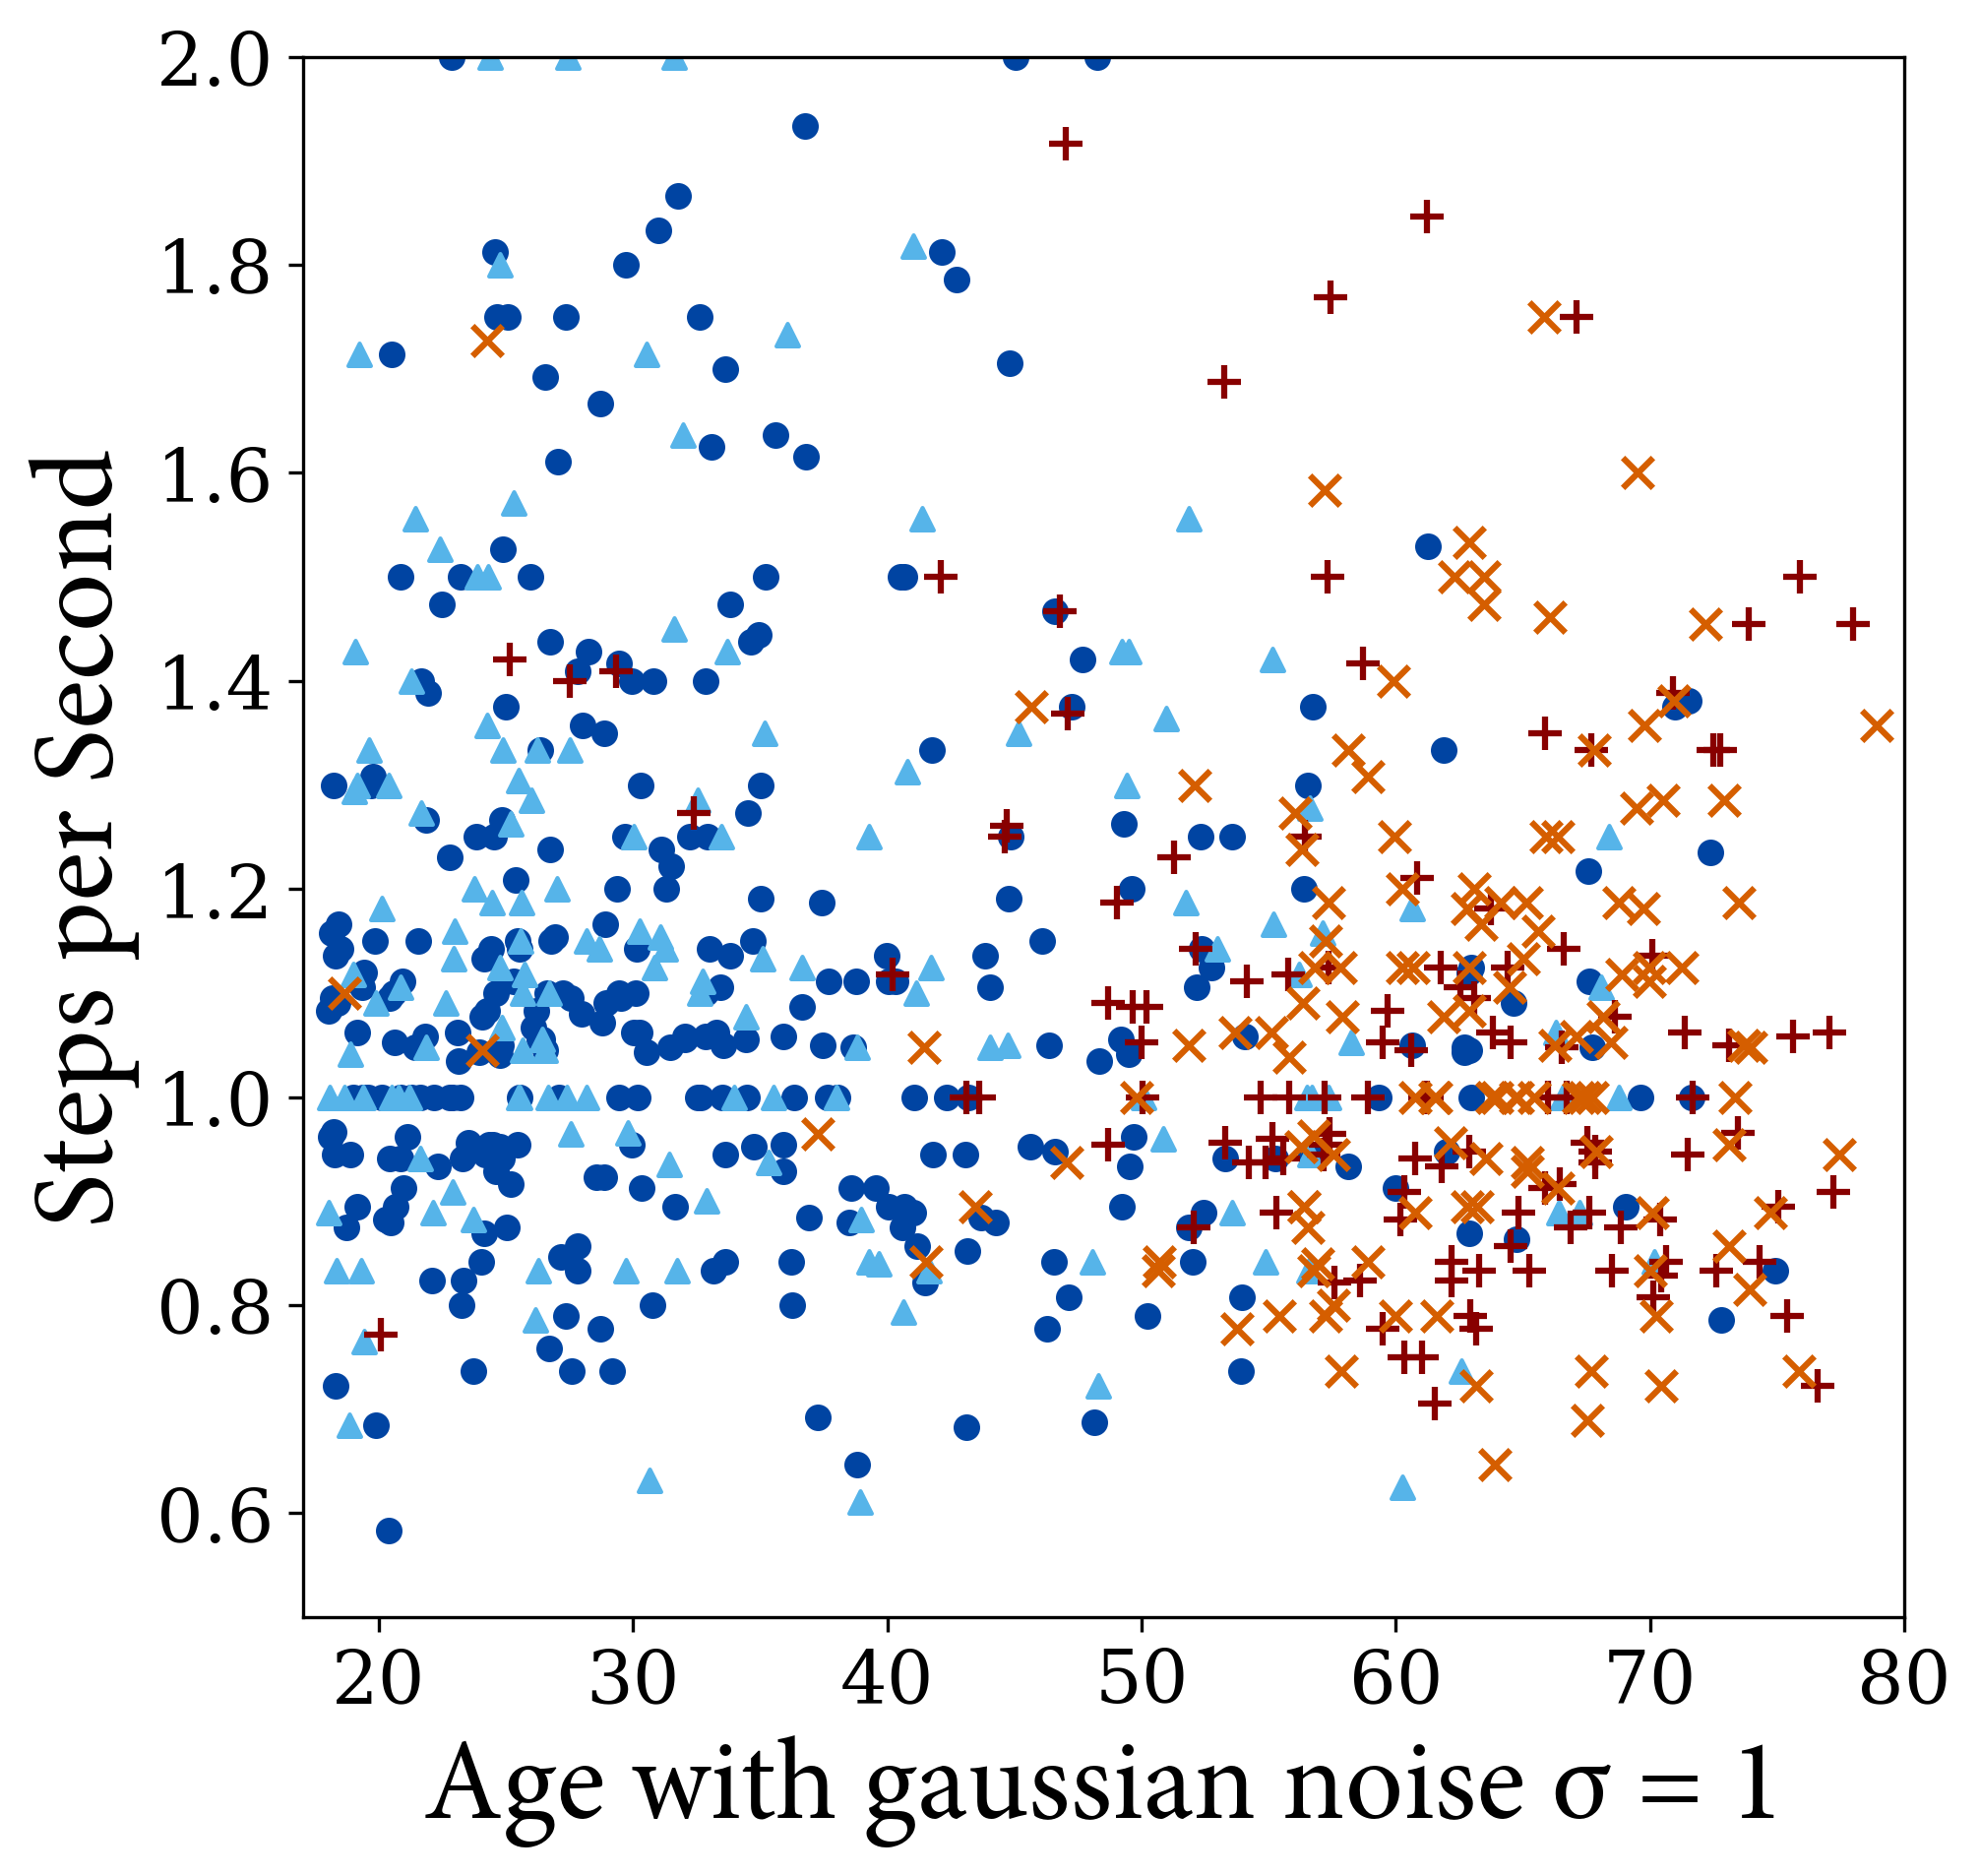
\includegraphics[width=0.92\linewidth]{stepspermin.png}
	\end{subfigure}%
	\begin{subfigure}{.5\textwidth}
		\centering
		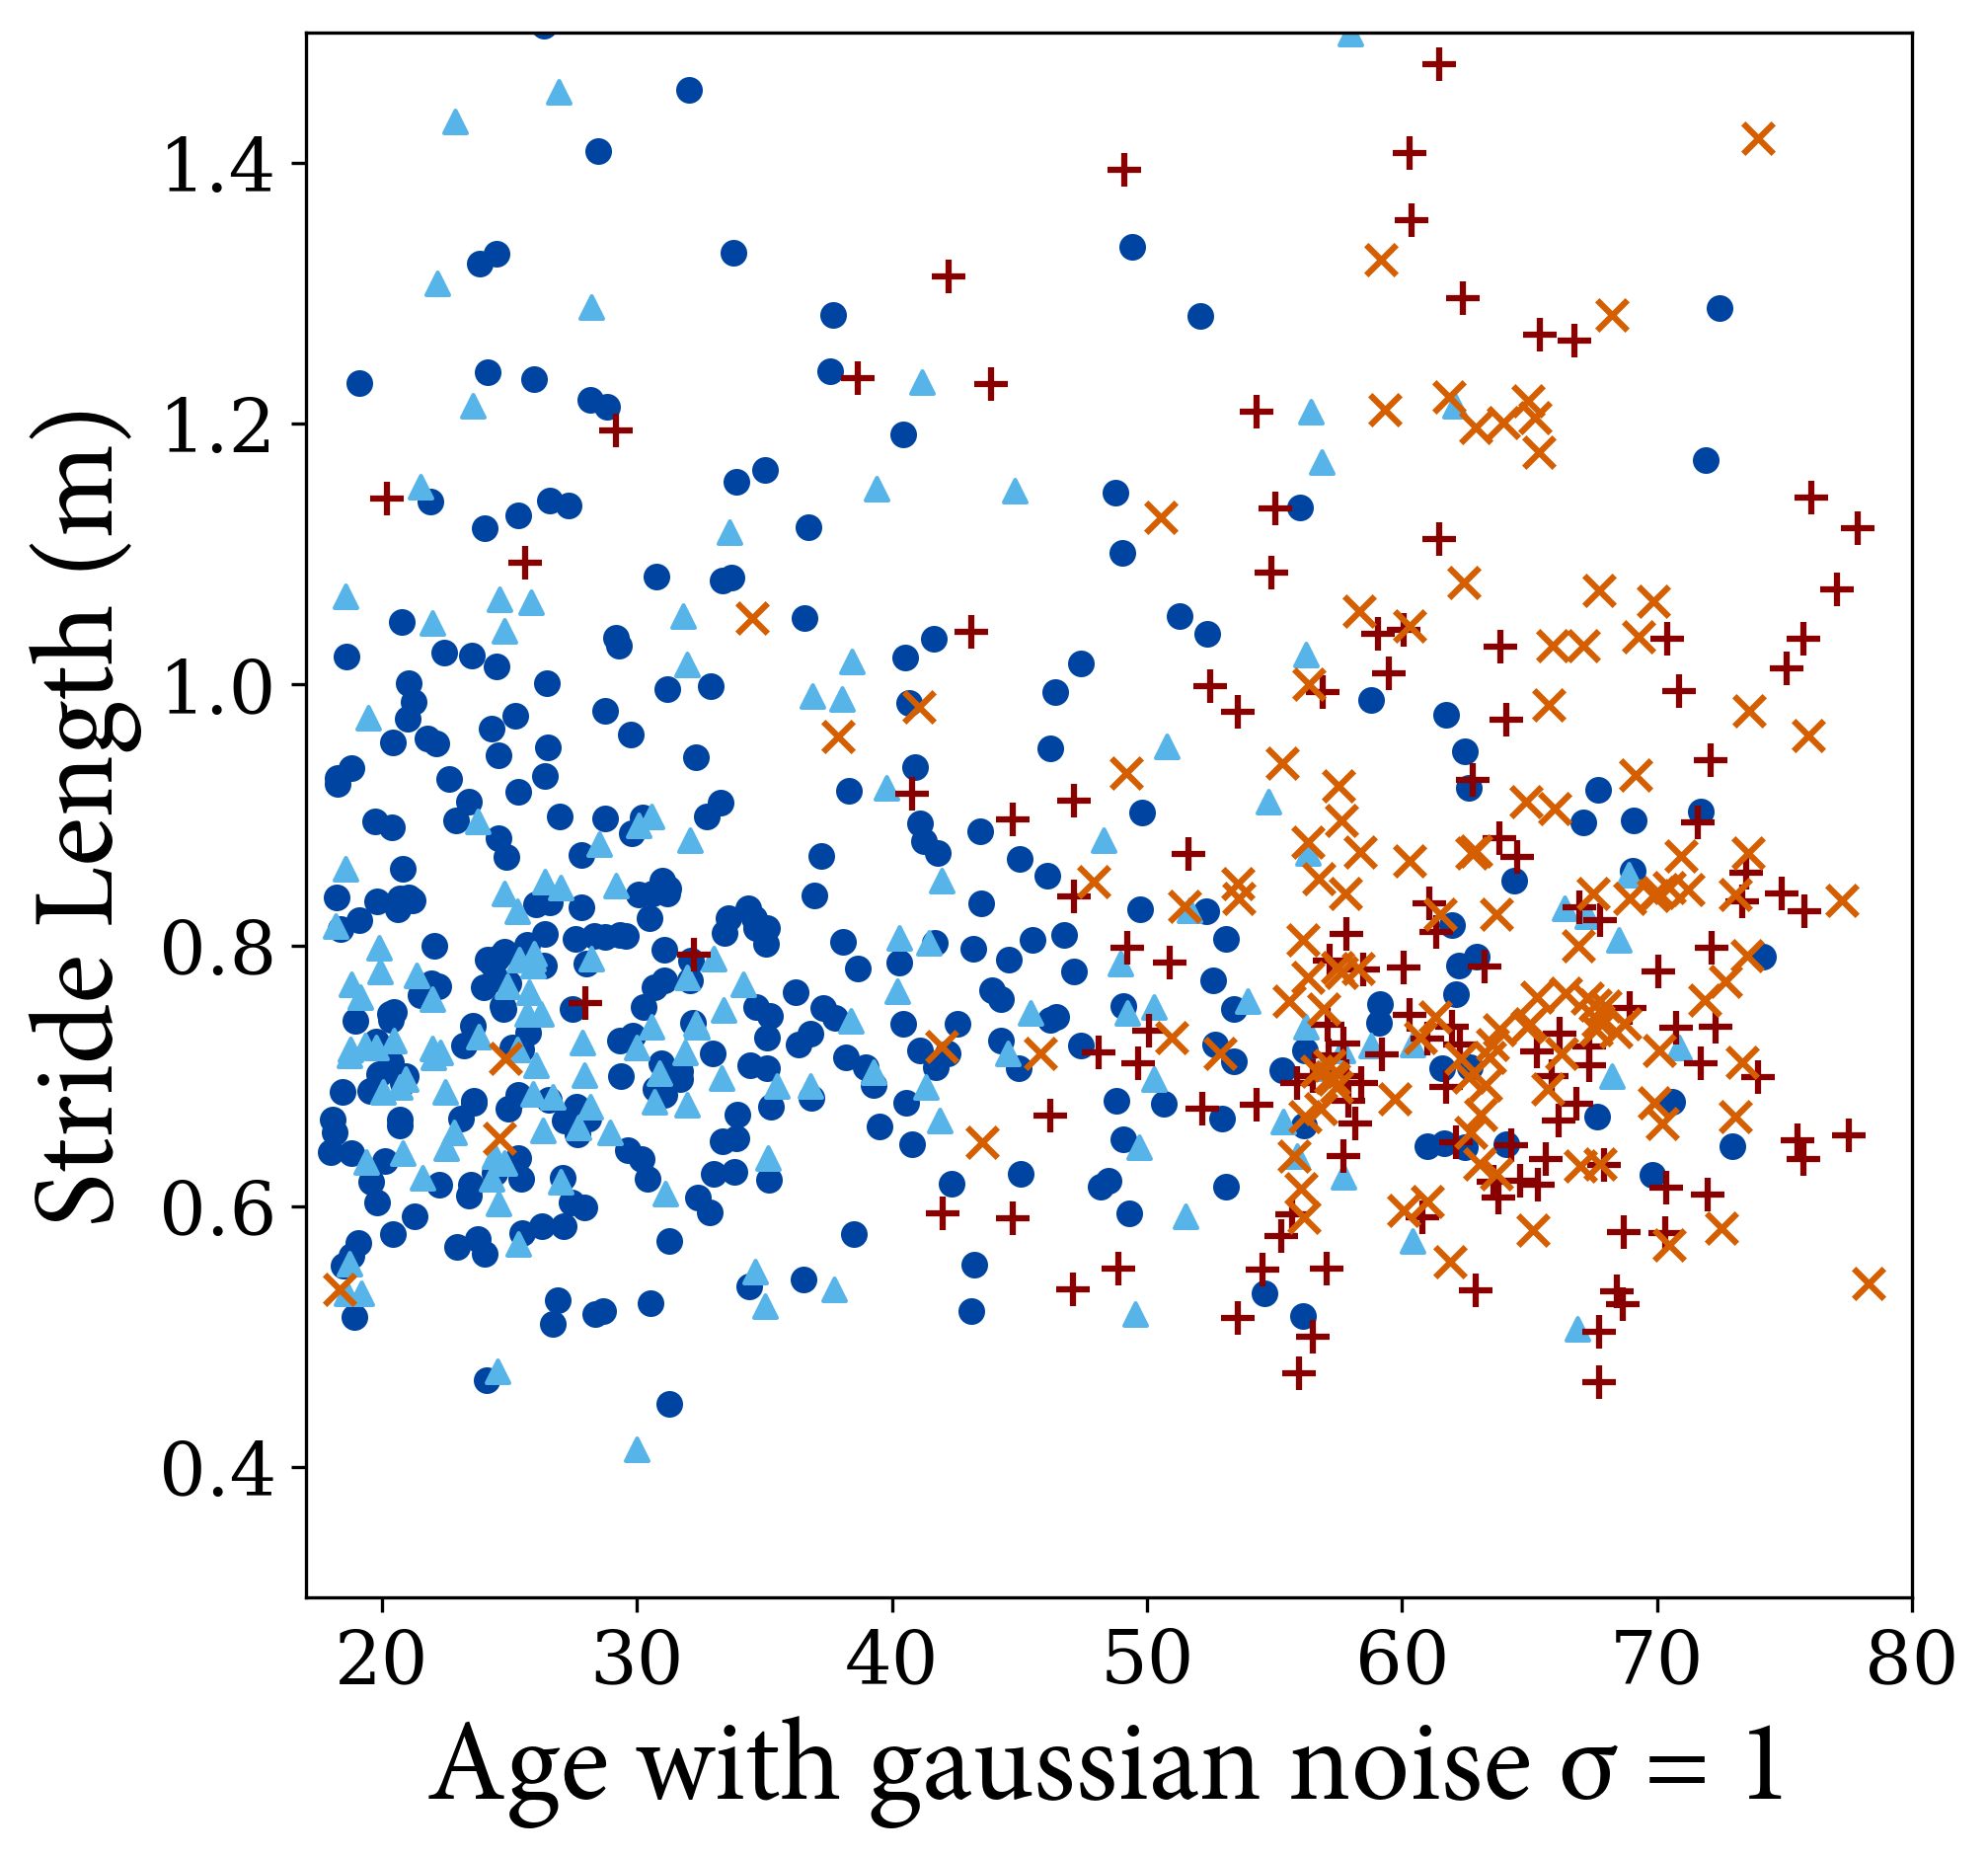
\includegraphics[width=0.92\linewidth]{stridelength.png}
	\end{subfigure}
	\caption{The average cadence and stride length of participants with PD is only marginally lower than age matched control.}
	\label{basicwalkvis}
\end{figure}

Basic walking features were calculated from the provided pedometer data, likely extracted from the implementation in Apple ResearchKit~\cite{mpower}. The estimation of steps and especially distance may not be accurate, accounting for additional variance in results. This is visualised in \textit{\hyperref[basicwalkvis]{Figure}}~\ref{basicwalkvis} and it is clear that these simple features are barely informative in diagnosis.


\begin{figure}[!htb]
	\centering
	\begin{subfigure}{.5\textwidth}
		\centering
		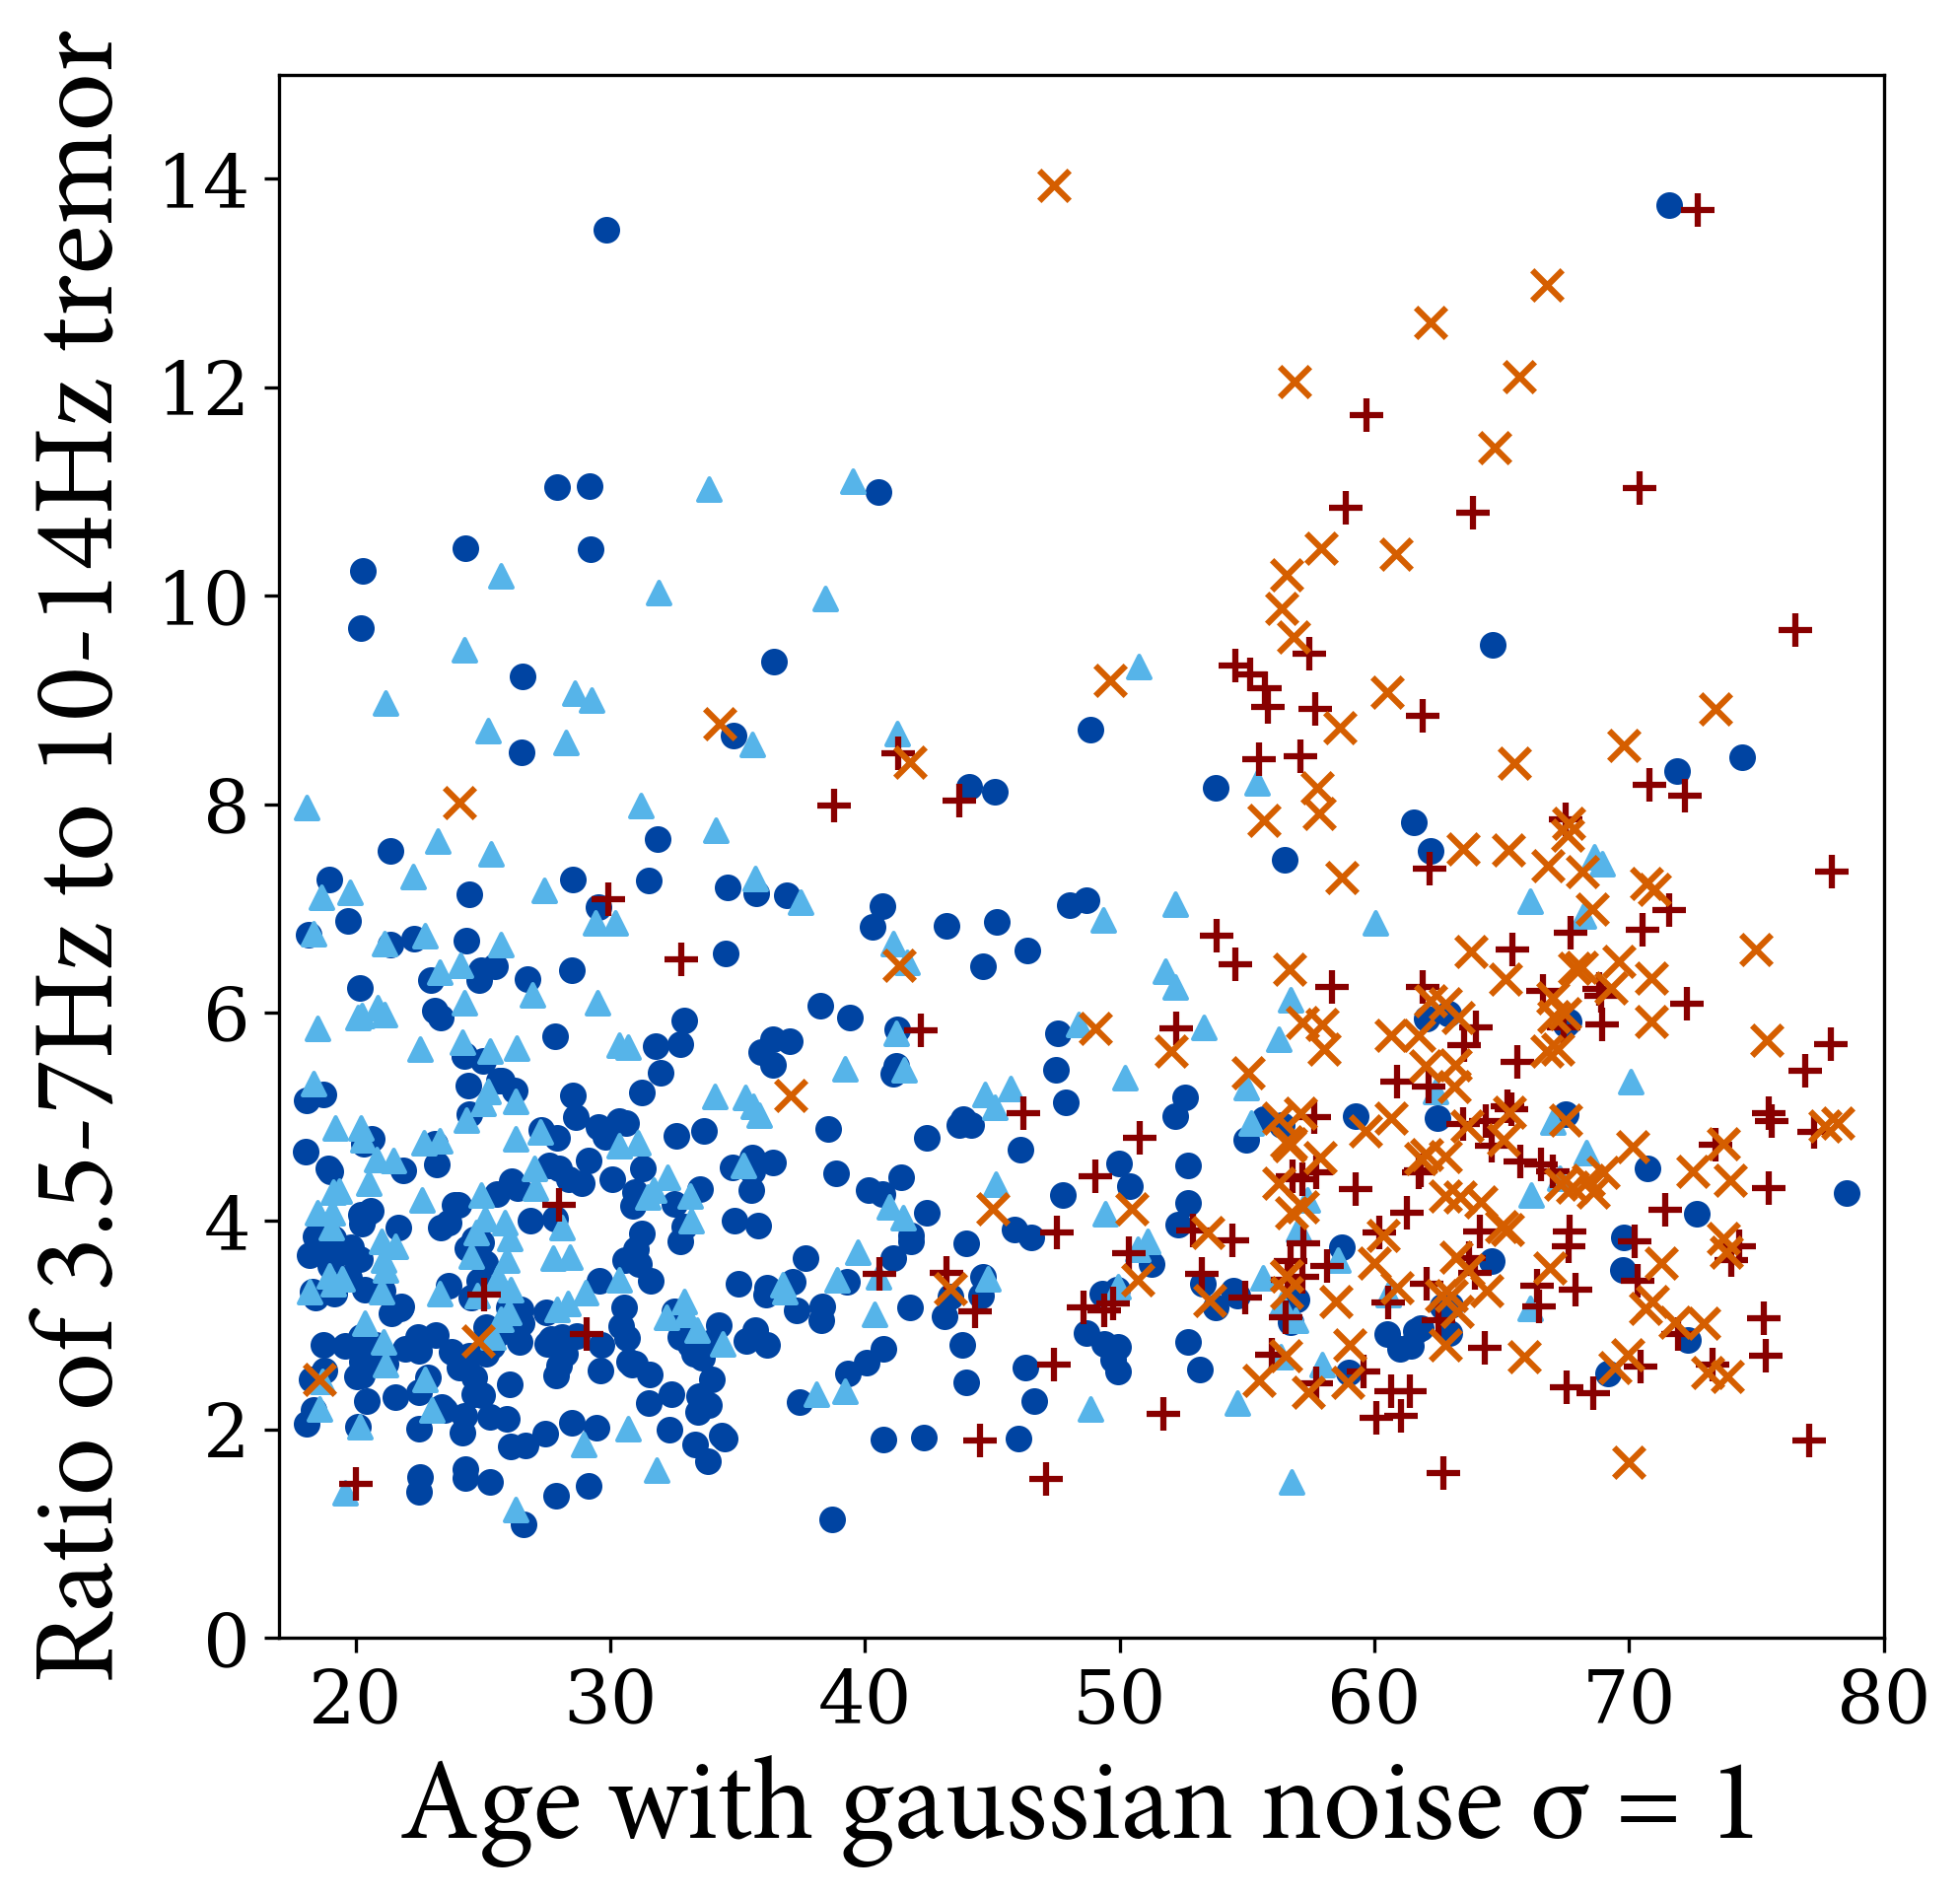
\includegraphics[width=0.92\linewidth]{resttremor.png}
	\end{subfigure}%
	\begin{subfigure}{.5\textwidth}
		\centering
		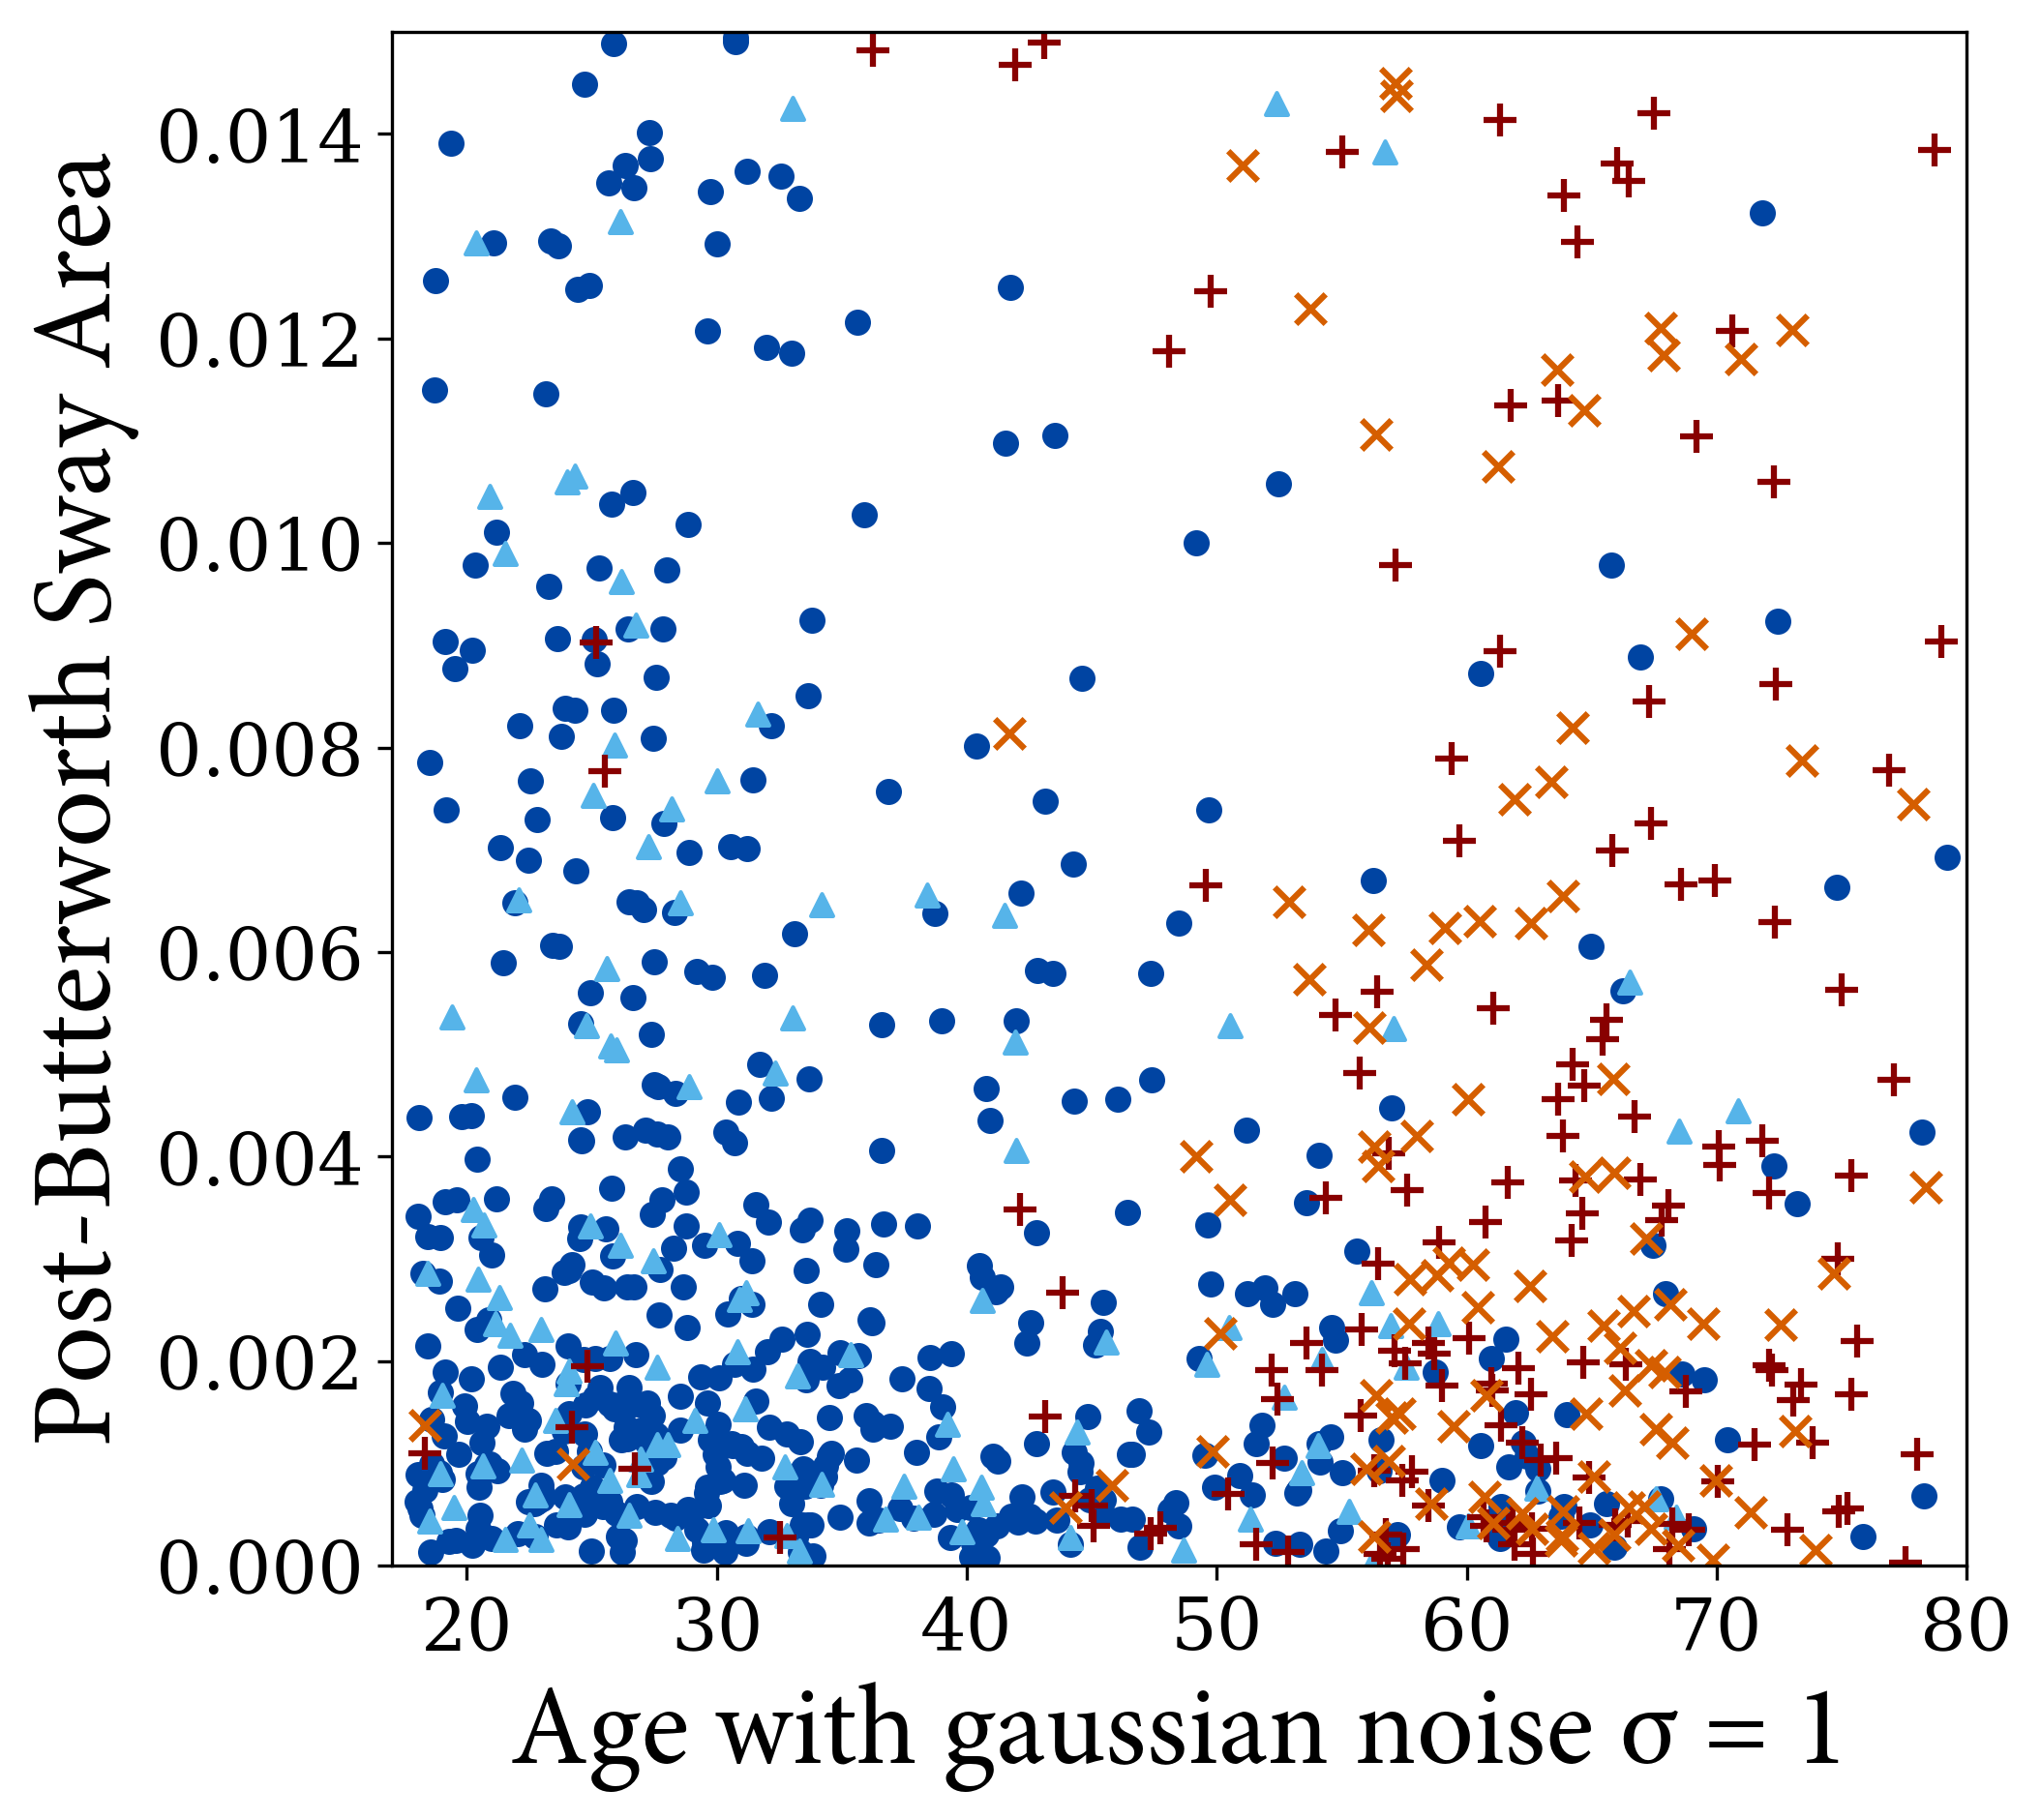
\includegraphics[width=0.92\linewidth]{bwswayarea.png}
	\end{subfigure}
	\caption{PD participants exhibit a definite increase in 3.5-7Hz tremor. The variance of sway area is high, and PD participants only exhibit a minor increase in sway area compared to age matched control. }
	\label{basicrest}
\end{figure}

The most common features used diagnosis of force plate and IMU data are tremor and postural sway. These are depicted in \textit{\hyperref[basicrest]{Figure}}~\ref{basicrest}. Visualising the ratio of tremor in the 3.5--7$\,$Hz bands (most commonly associated with PD) and 10--14$\,$Hz bands, there is a definite increase in Parkinsonian tremor. Post-Butterworth sway area (by bounding ellipse) is less informative and suffers from high variance.



\begin{figure}[!htb]
	\centerline{
		\centering
		\begin{subfigure}{.4\textwidth}
			\centering
			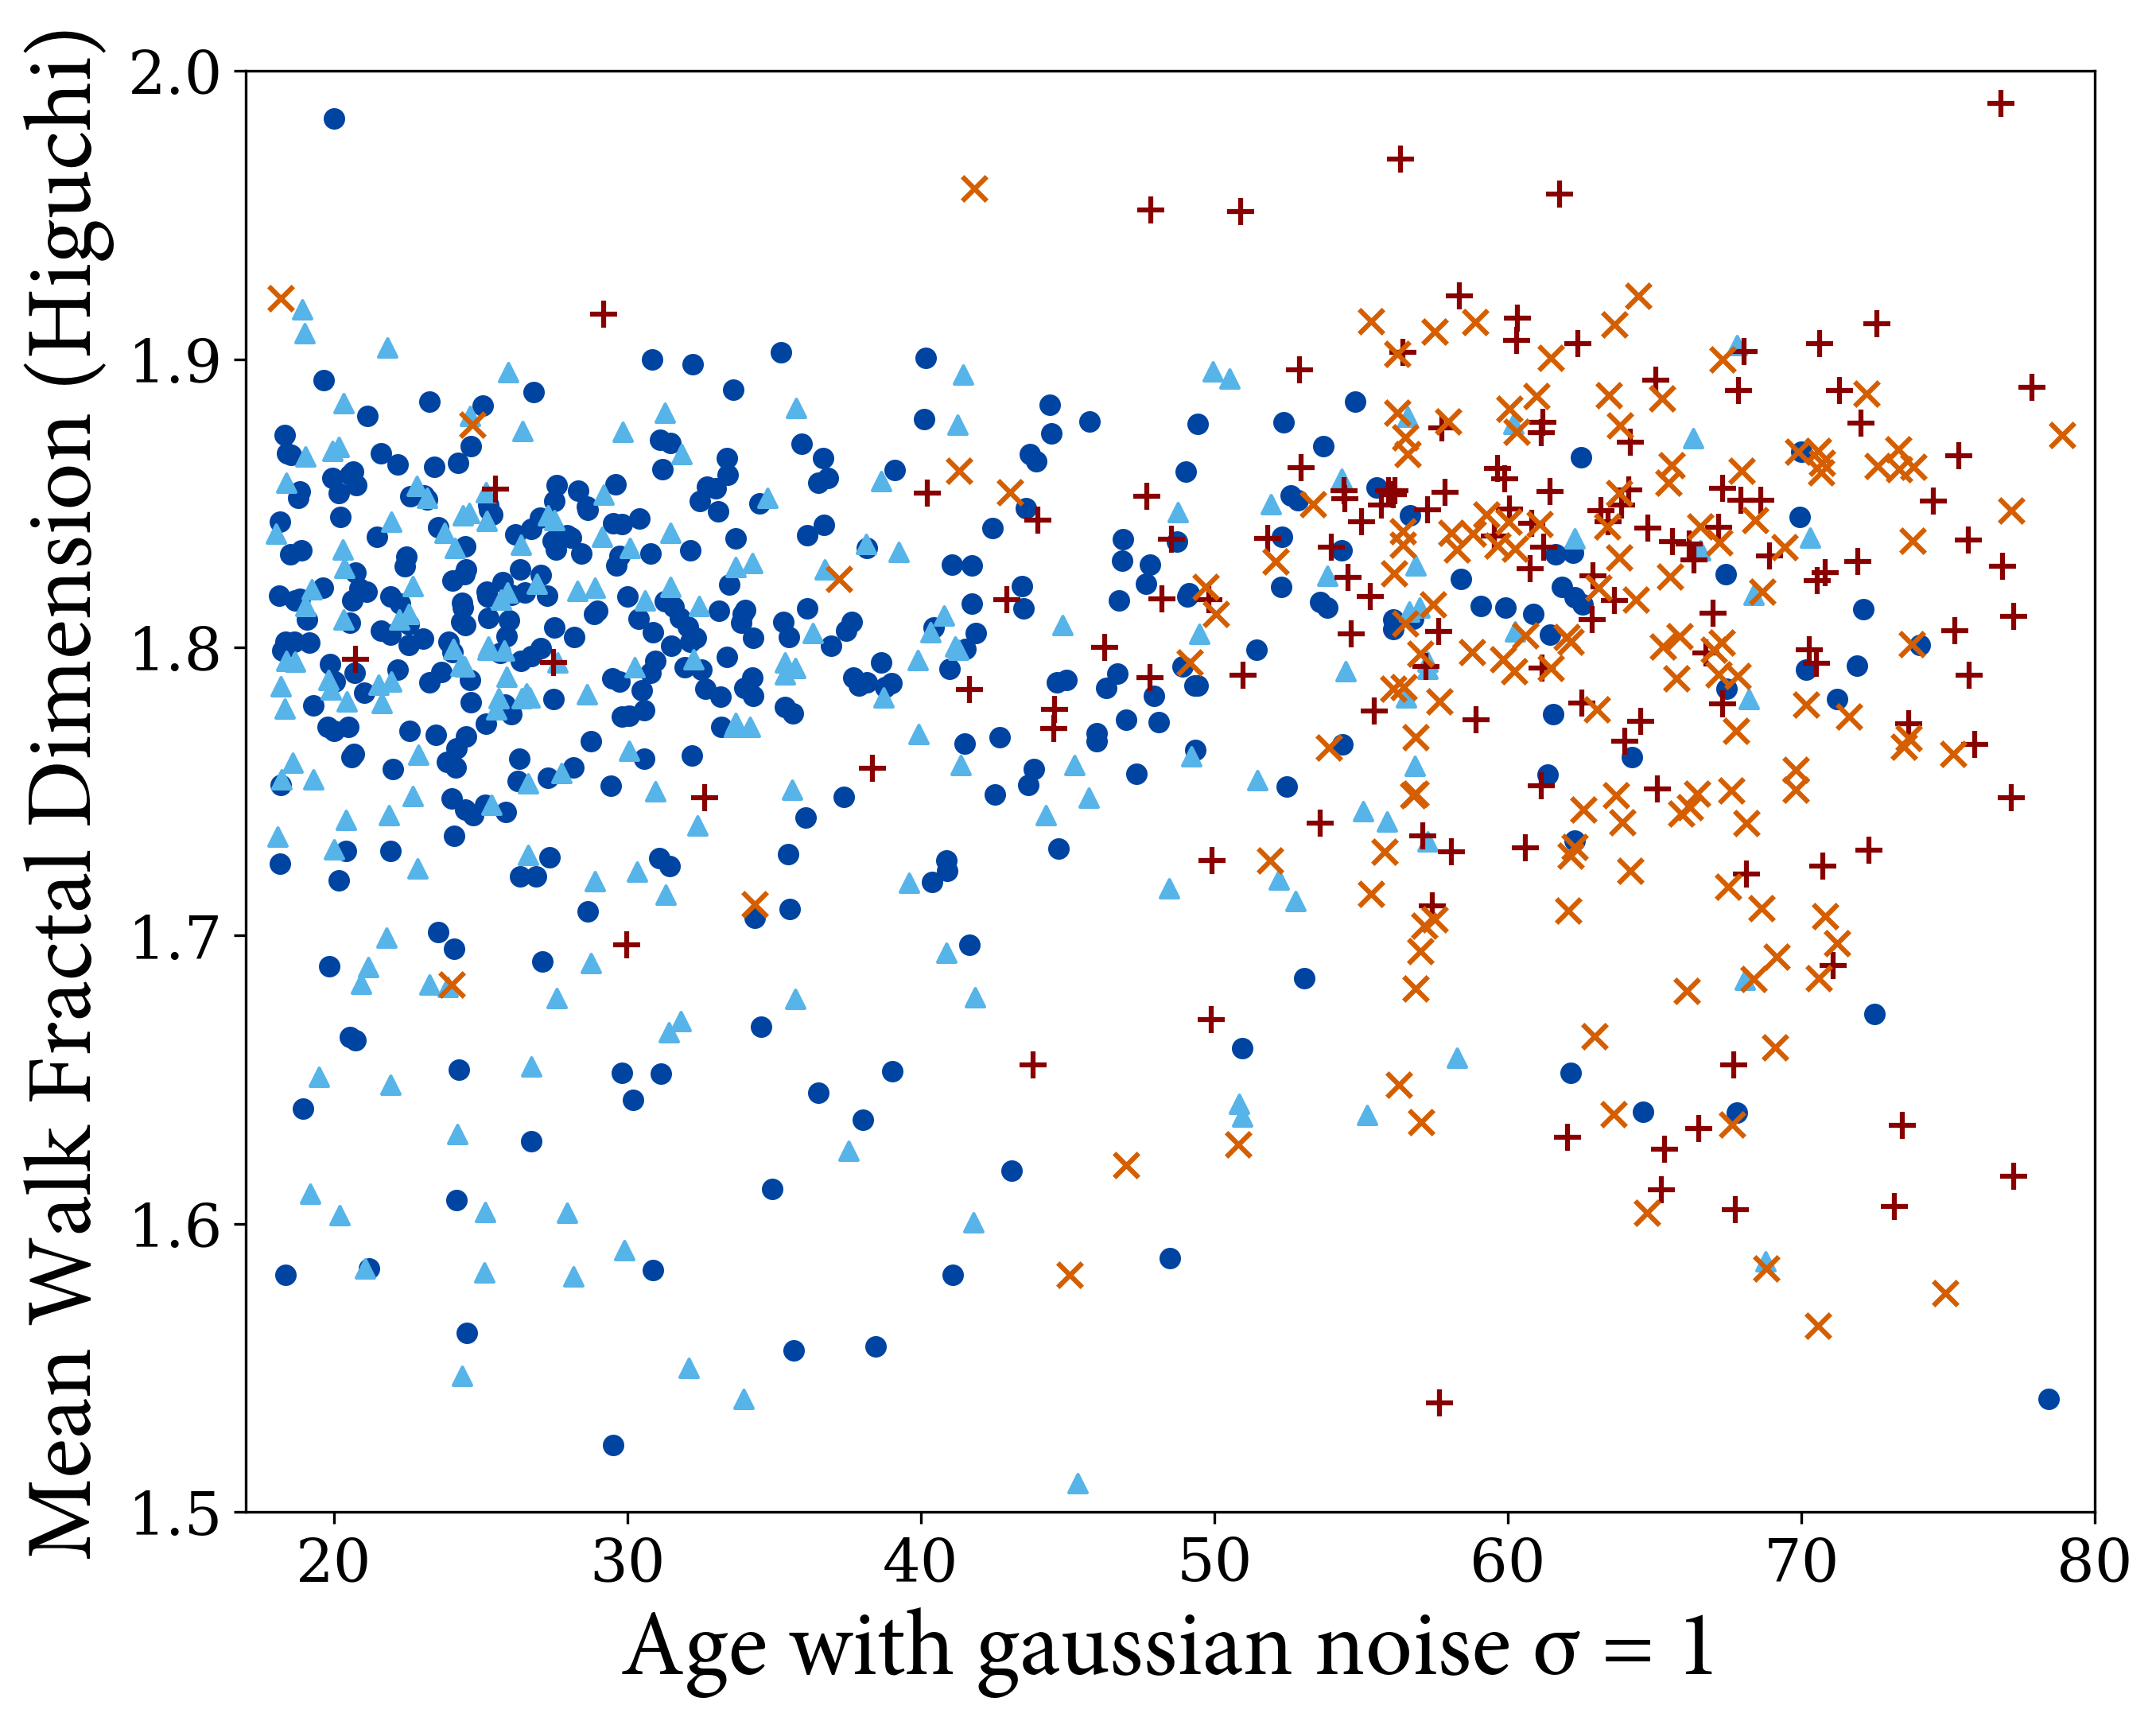
\includegraphics[width=0.96\linewidth]{fractal_dim_walk.png}
		\end{subfigure}
		\begin{subfigure}{.4\textwidth}
			\centering
			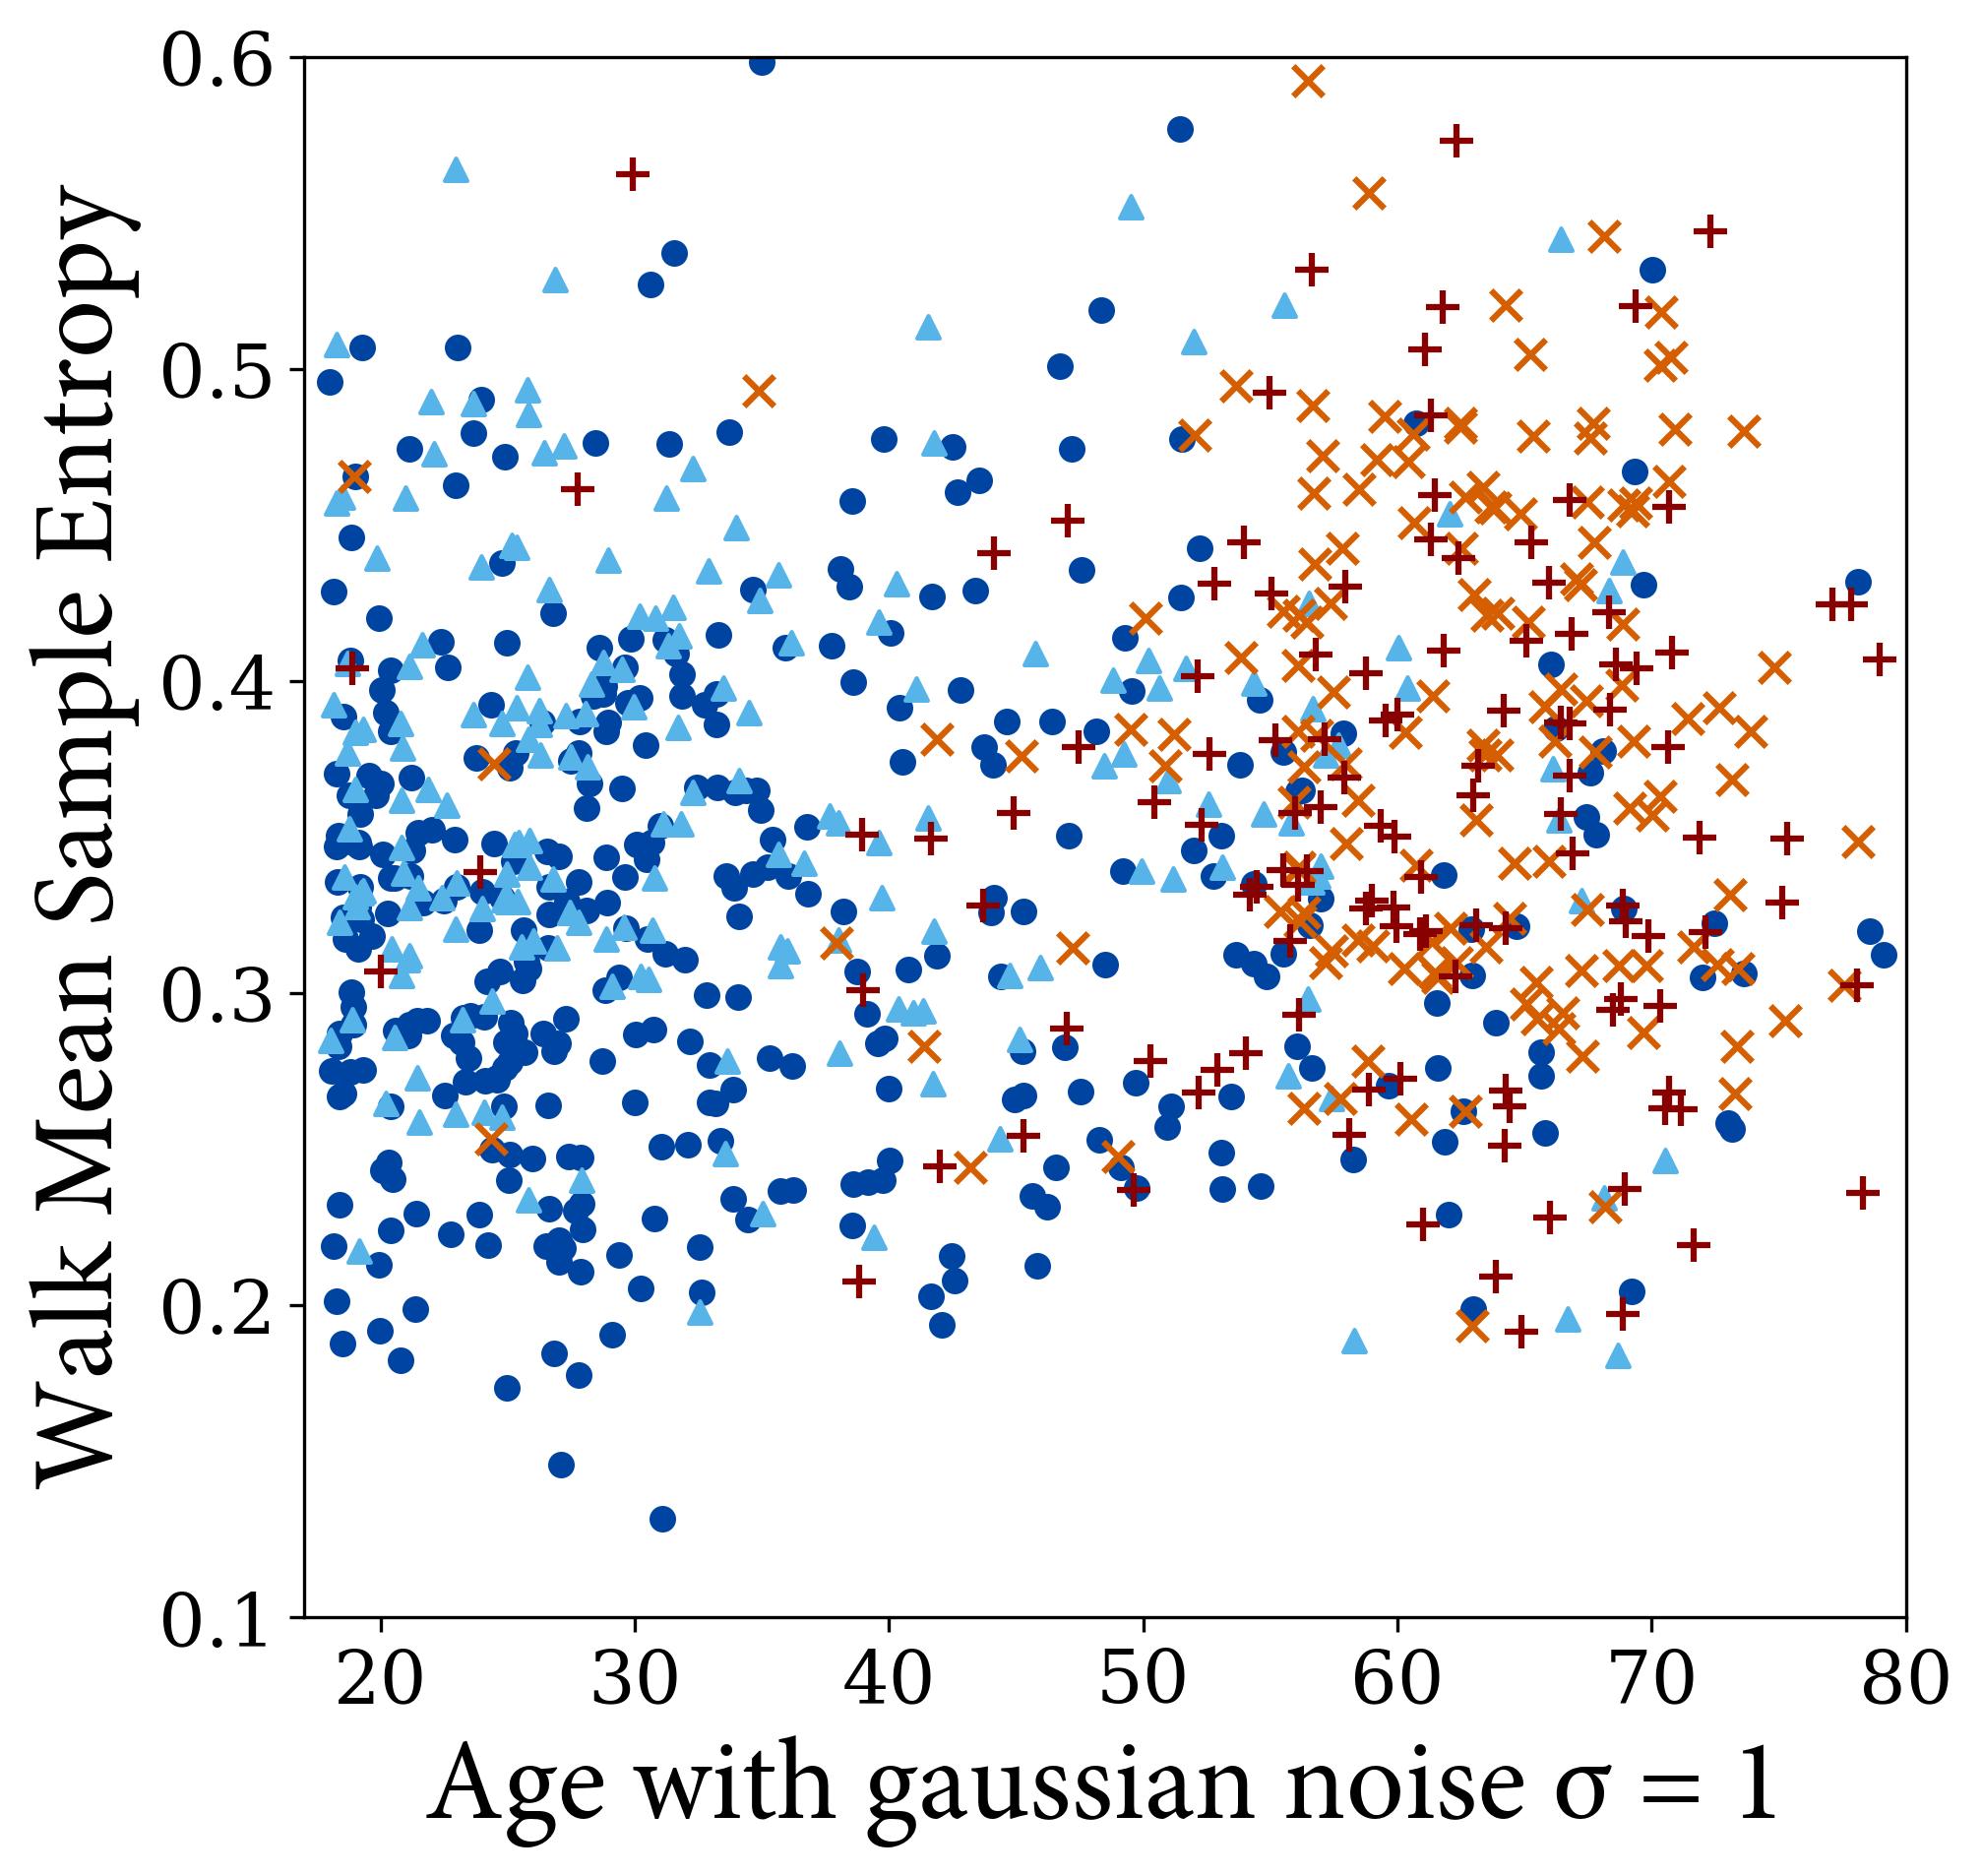
\includegraphics[width=0.96\linewidth]{walk_samp_ent.png}
		\end{subfigure}%
		\begin{subfigure}{.4\textwidth}
			\centering
			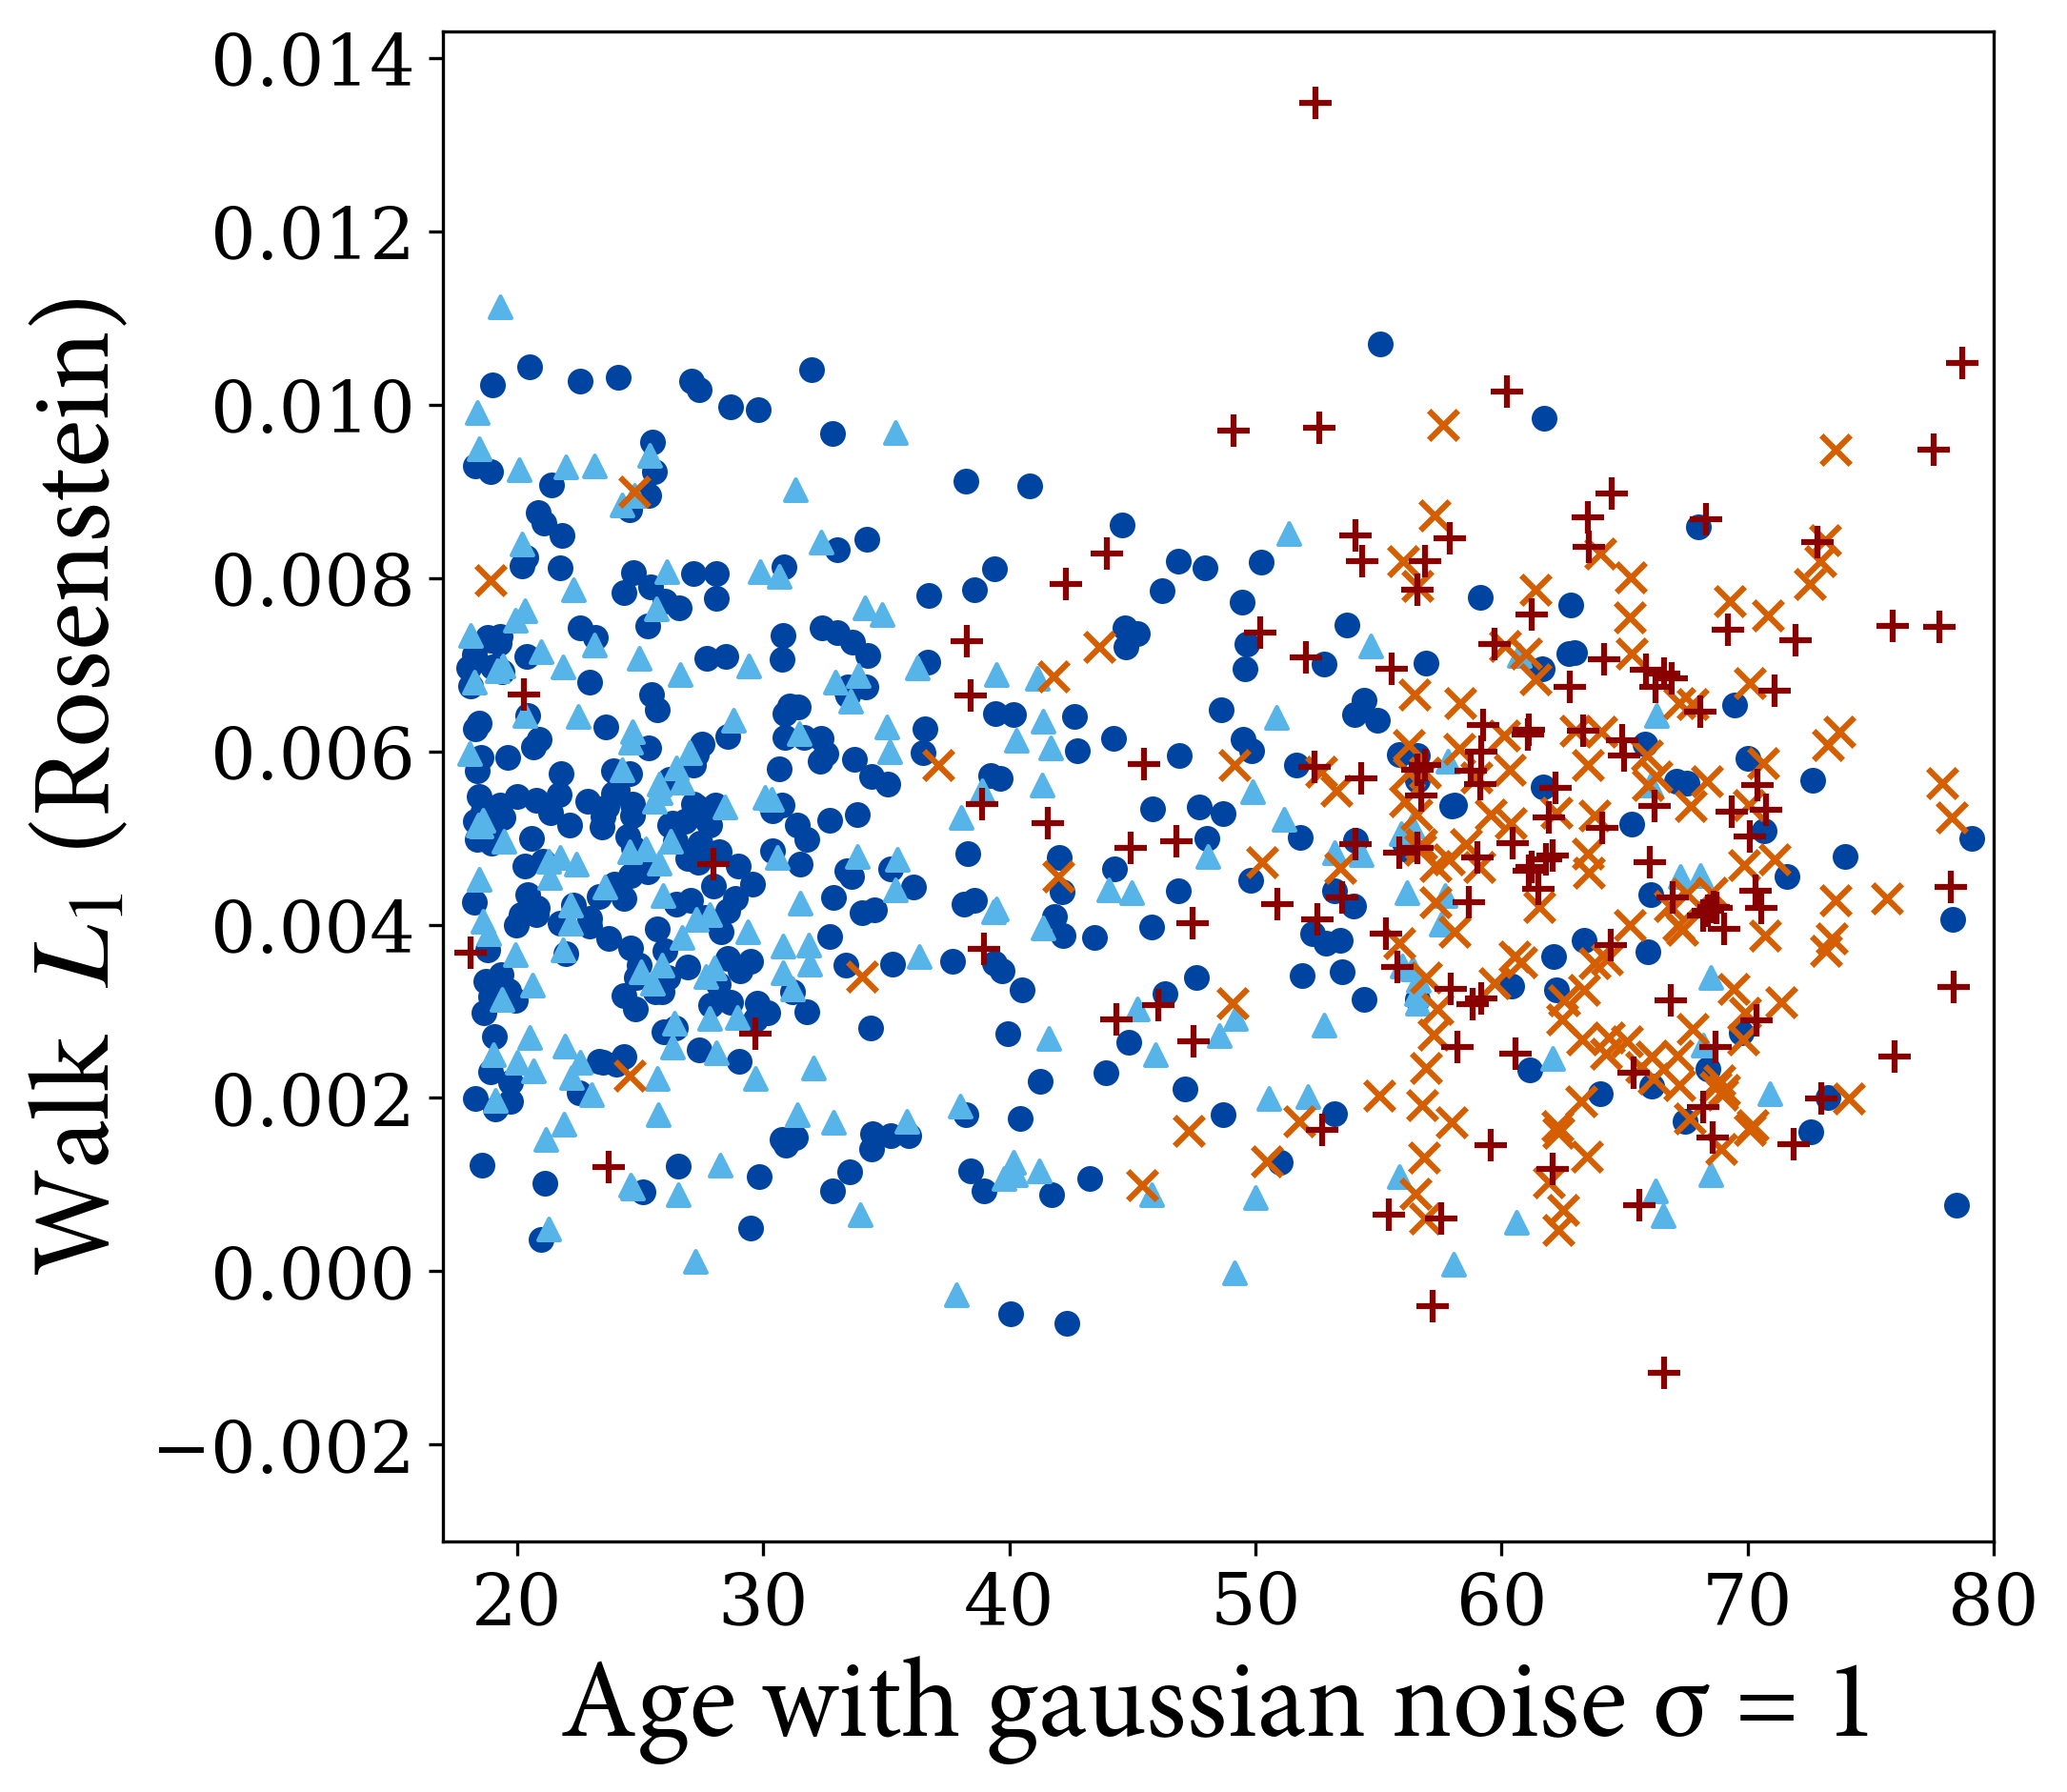
\includegraphics[width=0.96\linewidth]{walk_l1.png}
		\end{subfigure}%
	}
	\caption{The Higuchi fractal dimension and sample entropy are strong differentiators of PD, whereas $\lambda^*$ is uninformative.}
	\label{dynamicwalk}
\end{figure}

The novel features introduced in \textit{\hyperref[eegsigproc]{Section}} \ref{eegsigproc} are more suited at quantifying Parkinsonian gait. Three of them are visualised in \textit{\hyperref[dynamicwalk]{Figure}} \ref{dynamicwalk}. Fractal dimension and sample entropy are measures of the detail and complexity of a signal, and tend to be higher participants with PD --- especially females. This was a surprising result as we believed that the use of handbags would hinder the differentiability of PD.




As each gait cycle is significantly longer than a glottal cycle (speech), we would expect lower predictability in the movement task. The largest Lyapunov exponent is always positive; however, we find no statistically significant correlation between $\lambda^*$ and PD on both balance and walk data. This result contrasts with Howcraft et~al.~\cite{howcroft2014analysisgaitlyapunov} which showed a lower $\lambda^*$ in people with diabetic neuropathy (NP). This may suggest a possibility distinguish characteristics of PD and NP gait, but could also be attributed to the low sample rate of phone accelerometers which is unsuitable for estimating the Lyapunov Exponents~\cite{rosenstein1993practicallyapunov}. 



\subsection{Conclusions and Recommendations}
\label{visfeatrecommendations}
The wide variation in natural speech production makes it difficult to distinguish dysphonic speech. Many features are not invariant to the fundamental frequency of the speaker, as evident in differences between the male and female groups. Normalising these features with respect to $f_0$ may improve the applicability of these features.

Many features are sensitive to minor fluctuations in the signal and their value can change dramatically depending on the segment used, as will be shown in \textit{\hyperref[dataaugment]{Section}}~\ref{dataaugment}. The large fluctuations in value reduces their effectiveness as simple predictors; however, they may be valuable when the feature is calculated over short-time windows. Models such as CNNs or LSTMs (\textit{\hyperref[neuralnetworkintro]{Section}}~\ref{neuralnetworkintro}) can utilise the additional short-time temporal information to make more robust predictions. This would also solve the issue of some features being dependent on data length. Unfortunately this will not be explored due to computational limitations.

\begin{highlight}
	Making sense of each individual feature is a challenging task. Machine learning models are required to interpret the uncertainty of these features to obtain a reliable result.
\end{highlight}

As no individual feature can achieve good classification accuracy, machine learning models must combine multiple features to reach a reasonable level of performance. Traditional machine learning models are best suited to modelling features which are independent. They often perform worse when two features are correlated, despite there being additional information. Feature selection~\cite{skfeature} can be used in traditional machine learning models to reduce the impact of this. Models such as neural network are able to model non-linear relationships between features; however, training data may not be plentiful enough. In the following section, we will explore typical approaches to improving model performance in machine learning.
\newpage
\section{Improving Performance}
\label{dataaugment}
Three standard machine learning techniques for improving performance will be investigated: data augmentation, feature selection, and ensemble models.  These techniques have been shallowly applied to demonstrate their effectiveness --- additional computational resources is required to investigate the limits of these techniques. Data augmentation is applied to the phonation task, and feature selection and ensembling applied to the movement task.

\subsection{Data Augmentation for Phonation}
An quick examination of the features used for the phonation data showed that many were unstable, with around 10 per cent of them varying by at least $0.5$ standard deviations when computed over the same audio signal offset by different amounts. It was also clear that some features were not length independent, though resolving the length-invariance of features will not explored in this thesis.

We extracted seven 1.5 second samples from the recording, starting at the 1.5 to 4.5 second mark with a 0.5 second step size. The applicability of three simple methods of utilising the extra information is explored in \textit{\hyperref[speechboost]{Table}} \ref{speechboost}. \emph{Augmentation} involves using the additional samples as extra cross validation data. \emph{Merging} combined the 4 $\mathbb{R}^d$ vectors of features into a $\mathbb{R}^{4d}$ vector of features. Finally, \emph{Meanify} involves taking the mean of the features computed over the 4 samples. Note that this differs from `collapsing' by median in Neto et~al.~\cite{mpowerneto2017analysis} as the number of samples is fixed so bias from PD participants performing more recordings is avoided. Ensemble models are alternative techniques of utilising the extra data, and will be explored in \textit{\hyperref[spensemble]{Section}} \ref{spensemble}. 




\begin{table}[!htb]
	\caption{Cross validation results on full vocal feature set using a SVM on a 50PD:50C stratification of the data with various data augmentation techniques.}
	\label{speechboost}
	\centering
	\begin{tabular}{@{}rcccc@{}}
		&  Original & Augmented & Merged & Mean \\ \midrule
		Accuracy [\%]    &      $72.2\pm3.1$ &                       $76.9\pm1.0$                                  &     		$70.3\pm2.8$
		&						$73.3\pm3.0$\\ \midrule
		Sensitivity [\%] &       $69.7\pm4.3$ &                       $73.5\pm1.5$                                  &    		$69.6\pm4.7$
		&					    $69.9\pm4.9$\\ \midrule
		Specificity [\%] &      $74.8\pm4.7$ &                       $80.3\pm1.4$                                  &    		$71.1\pm4.5$
		&					    $76.9\pm4.3$\\ \midrule
		AUROC [\%]         &      $78.3\pm2.9$ &                       $84.0\pm1.1$                                  &     		$75.9\pm0.3$
		&				 		$80.4\pm2.7$\\ \midrule
	\end{tabular}
\end{table}

Augmentation and mean exceed the performance of the original feature set at a Bayes factor of $10^{23}$ and $10^3$ respectively. As expected, merging does not perform well with a SVM and shows the applicability of feature selection --- even in models as robust as SVMs. Data augmentation strategies evidently provide a viable solution to overcoming the low data quality in the mPower dataset. 

\begin{highlight}
Data augmentation was extremely effective, implying that performance can be significantly improved with more data.
\end{highlight}

Recurrent and convolutional networks can utilise additional temporal and variance information to improve predictions. However, the neural network architectures we applied achieved similar performance to the augmented SVM. Likely, more than seven segments are required to fully utilise the benefits of these models.



\subsection{Feature Selection and Ensembles for Accelerometer}
There are 431 numerical features used to classify accelerometer data, and many are likely redundant. Most signal processing measures are only well defined for one dimensional signals and the accelerometer provides three ($x$, $y$, $z$) dimensions of data. Although information is gained from computing measures over all dimensions, it is difficult for most machine learning models to utilise this information. It is likely that the additional variability in the axis, and the correlated nature of the data will reduce the performance of most classifiers. The effect of taking the Euclidian norm on classification accuracy is depicted in \textit{\hyperref[accelerometernorm]{Table}} \ref{accelerometernorm}.

\begin{table}[!htb]
	\caption{Results of taking the norm for features extracted over $(x,y,z)$ dimensions with a SVM. The normed features perform worse than the full feature set ($BF=41$).}
	\label{accelerometernorm}
	\centering
	\begin{tabular}{@{}rcccc@{}}
		&  DREAM & Novel Only & Both (full) & Both (normed) \\ \midrule
		Accuracy [\%]    &      $63.8\pm3.9$ &                       $66.0\pm4.0$                                  &     $68.8\pm3.7$
		&						$67.7\pm4.0$\\ \midrule
		Sensitivity [\%] &      $62.6\pm5.4$ &                       $61.8\pm5.7$                                  &     $67.2\pm5.3$
		&					    $65.4\pm6.1$\\ \midrule
		Specificity [\%] &      $65.0\pm5.7$ &                       $70.2\pm1.9$                                  &     $70.5\pm5.4$
		&					    $70.0\pm5.2$\\ \midrule
		AUROC [\%]         &      $72.1\pm4.8$ &                       $71.3\pm4.5$                                  &     $74.8\pm4.1$
		&				 		$74.0\pm4.0$\\ \midrule
	\end{tabular}
\end{table}

Somewhat unexpectedly, the normed feature set performs on par or worse than the full feature set. This implies that a SVM classifier can take advantage of the additional data provided by the individual dimensions. 


Features were extracted over the raw and high-passed balancing signal. Likely, only one of these will be redundant. Many measures such as the Higuchi and Petrosian fractal dimension are also correlated, and performance can be improved in some models by removing these redundant features. We evaluated a number of state of the art feature selection methods (\textit{\hyperref[featureselection]{Table}} \ref{featureselection}) and with a RBF SVM and sparse Gaussian process (GP)\footnote{Kernel based models are computationally infeasible for large datasets. \emph{Sparse} methods involve learning over a representative set of the full data~\cite{sparsematrix}. SVMs are inherently sparse, and sparse GPs~\cite{sparsegp} are an approximation of a full GP.} optimised over the 204 feature normed set (hyperparameter search for each feature subset was computationally prohibitive and the parameters of the normed model would be a good midway for small and large feature sets).


\begin{figure}[!htb]
	\centering\centerline{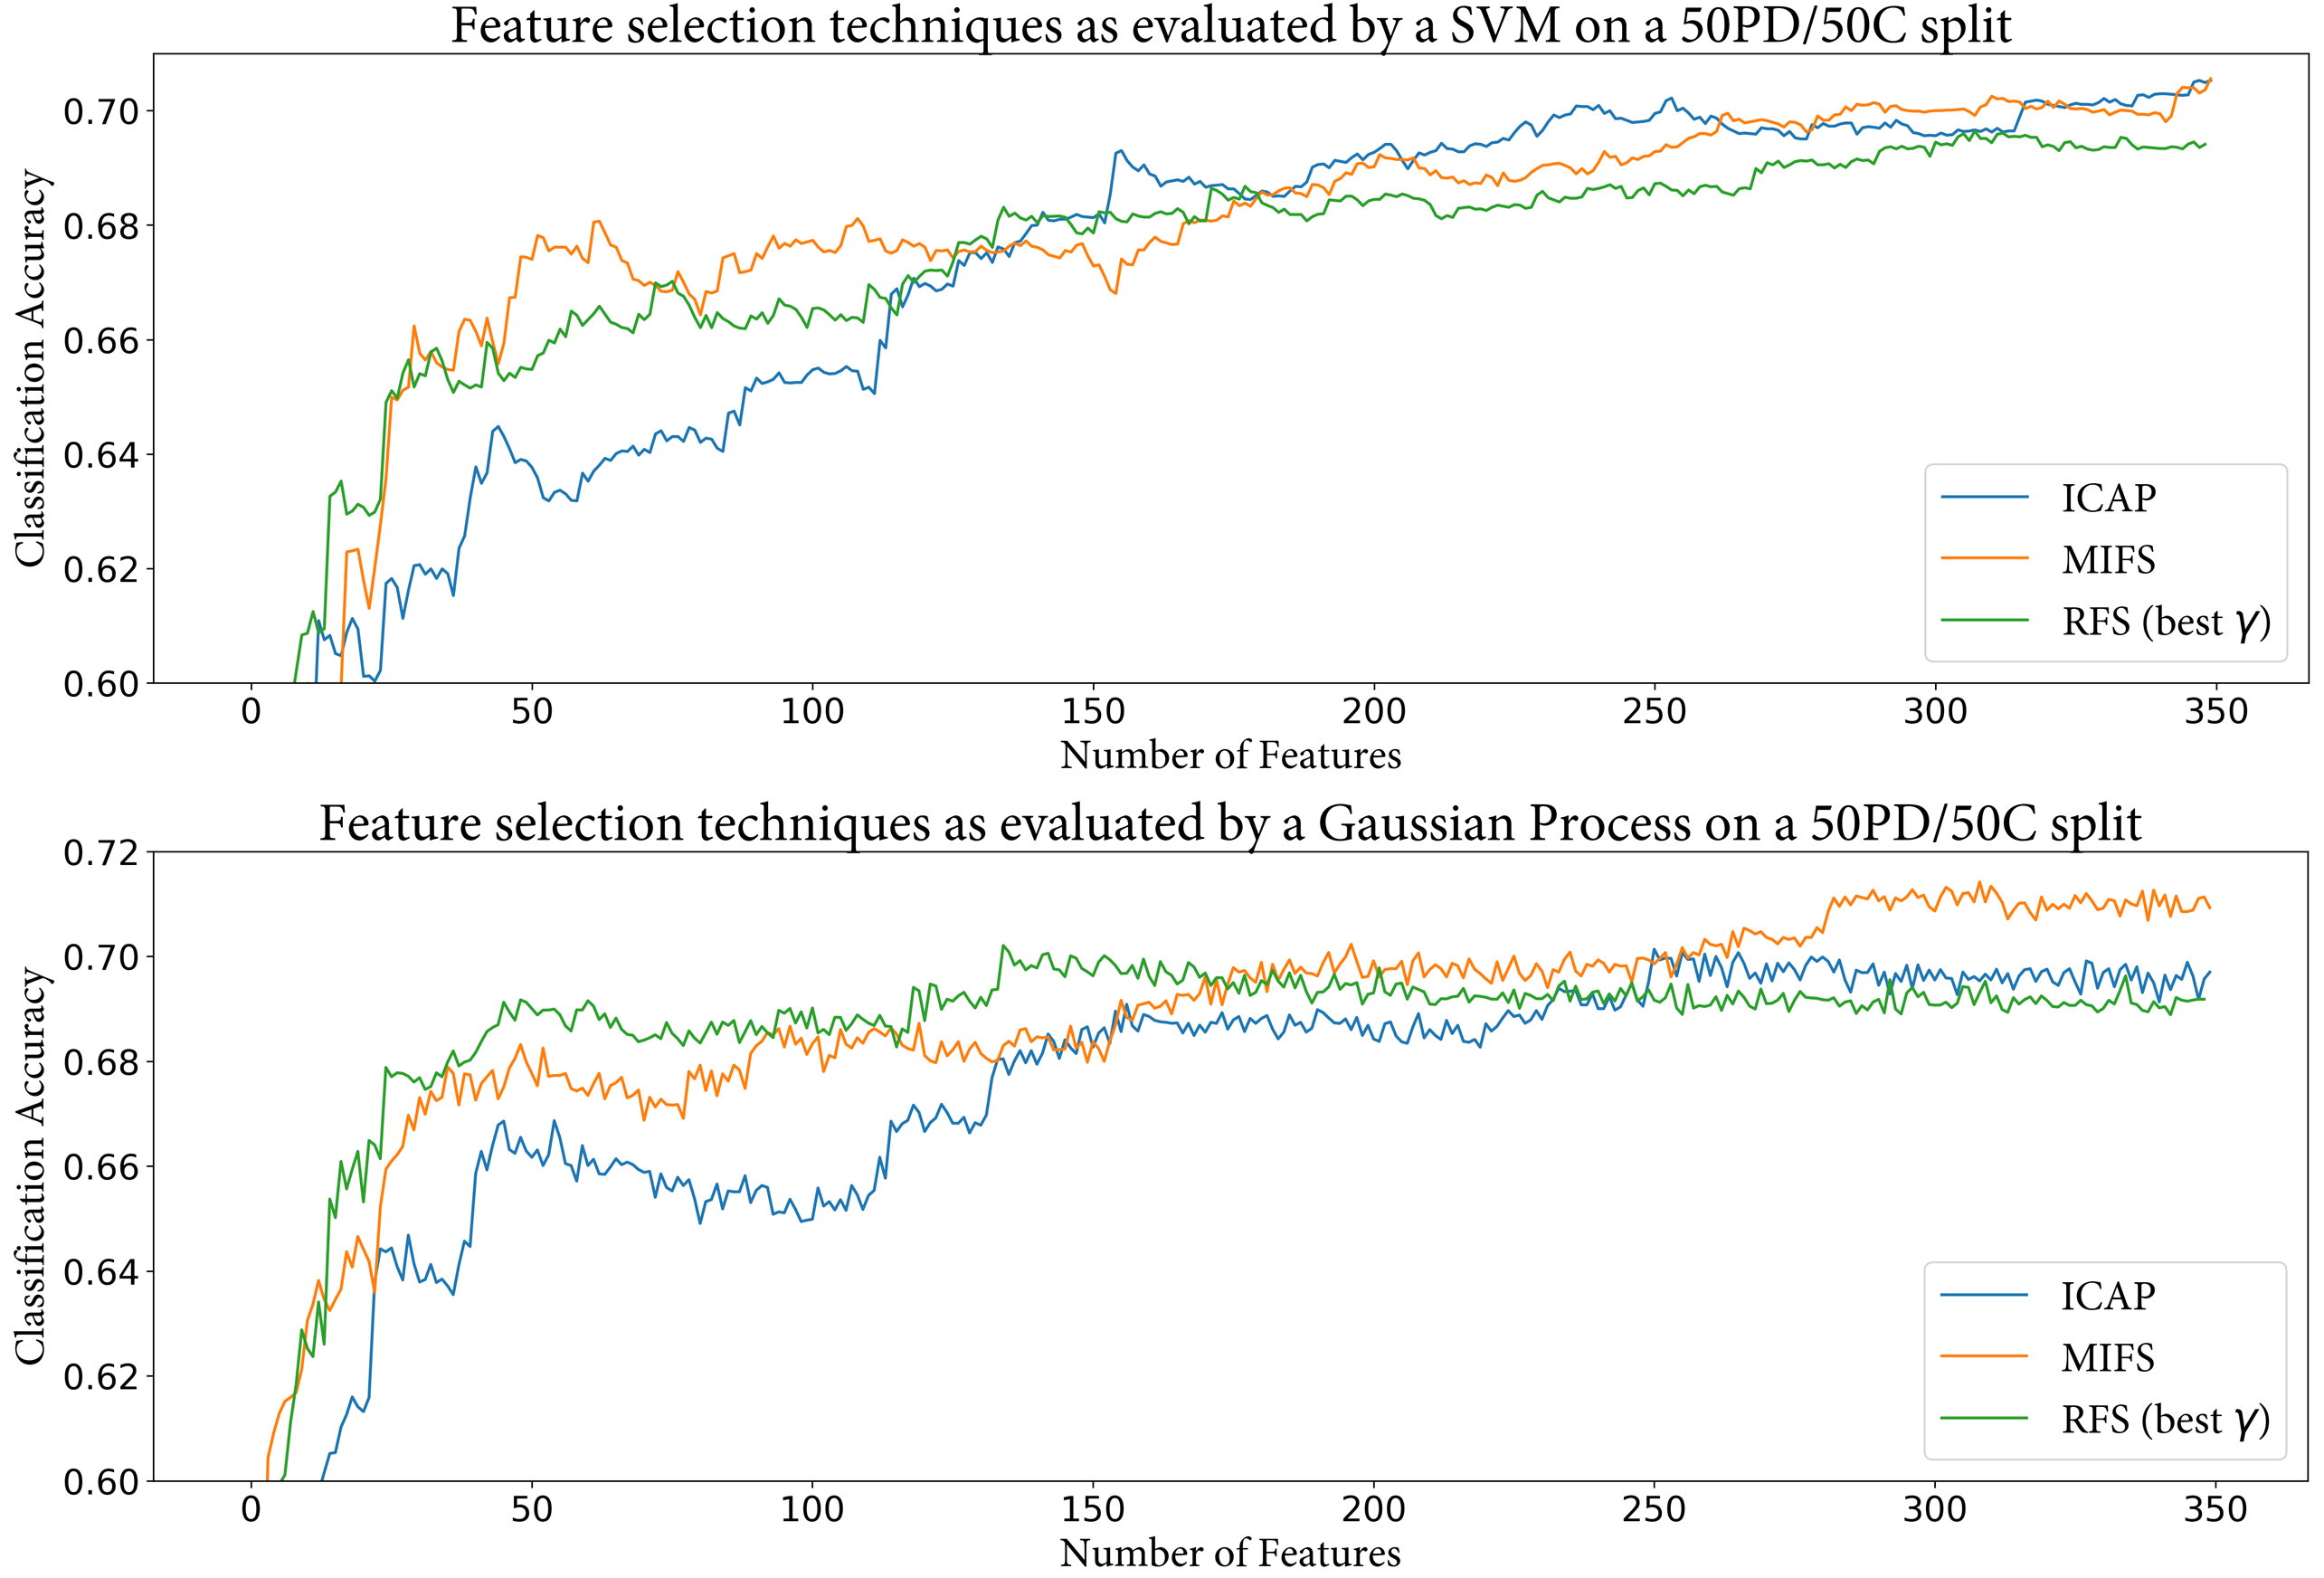
\includegraphics[width=1.07\linewidth]{fsel_accel.png}}
	\caption{Most notable 3 feature selection techniques evaluated with pre-optimised SVM and sparse GP on the full accelerometer feature set. Information theoretic filters generally performed best along with $l_{2,1}$ norm minimisation based RFS.}
	\label{accelerometerfsel}
	\vspace{-0.5em}
\end{figure}

The best feature subsets exhibited a correlation between performance and the number of features used. This is likely due to sparse GPs and SVMs being reasonably robust to redundant and correlated features (unlike na\"{i}ve Bayes), and the natural uncertainty of the features as predictors. With the information theoretic based feature selection techniques, there are `spikes' in classification accuracy --- suggesting that there exist features which appear uninformative, but are informative when combined with other features. 

The performance of the best 150--350 feature subsets appeared to exceed the performance over all features (\textit{\hyperref[accelerometernorm]{Table}} \ref{accelerometernorm}), despite the lack of hyperparameter search. This could be an artefact of using 3-fold cross validation rather than 10-fold. We evaluated the final MIFS 350 feature subset with our standard methodology, finding no significant performance improvement over the full feature set. This reinforces the need for robust model evaluation before accepting a result.

\begin{highlight}
	The feature reduction techniques explored were not very effective. This is primarily due to the inherently high uncertainty and correlation of most features.
\end{highlight}
\newpage
\label{spensemble}
An interesting observation is that the GP and SVM differ in performance on the same feature subsets. Although ICAP performed well with a SVM, CIFE was more suitable for the GP. Similarly, the small ~50 feature subsets selected by RFS performed exceptionally with the GP whereas they were average when used by the SVM. This suggests that each model uses a different set of information to make classifications, and performance could potentially improve with a more complex model. 

Noting this observation, we investigated the performance of an ensemble model consisting of seven independent predictors: A SVM, Gaussian process, random forest, k-nearest neighbour (with $k=3$) classifier, and neural networks with three, five and seven hidden layers. All models chosen were suited to the task, diagnosing PD within $\pm2$ per cent accuracy of each other.

The goal of an ensemble is the combine multiple machine learning models to create a more robust one. Ensembling techniques such as bagging and boosting~\cite{adaboost} are more suitable for ensembling `weak' learners~\cite{ensembleml}. When strong predictors are used, it is more appropriate to aggregate their predictions, either by averaging (\emph{voting}) or using another model (\emph{stacking})~\cite{stackregression}.

Building on stacking, \textit{Feature-Weighted Linear Stacking} (\emph{FWLS}) assigns a weight to each feature and model combination~\cite{fwls}. The motivation of FWLS is that in complex feature spaces, models make predictions with different sets features. This hypothesis is likely, due to the varying performance of the SVM and GP on different subsets of features. FWLS was the technique used to ensemble the winning model of the prestigious ``Netflix prize''~\cite{netflixprizebellkor}.


A RBF Gaussian process was chosen to aggregate the models in stacking and FWLS based ensembles. Gaussian processes are inherently probabilistic classifiers and are suitable for making decisions in situations of high uncertainty. Although the Netflix prize was won using gradient boosted trees~\cite{gradientboosting}, Gaussian processes worked better in our problem. The results of these ensembling techniques are presented in \hyperref[ensembles]{Table} \ref{ensembles}.


\begin{table}[!htb]
	\caption{The results of various ensembling techniques over a combination of SVM, Gaussian process, random forest, k-nearest neighbour, and a three, five and seven layer neural network.}
	\label{ensembles}
	\centering
	\begin{tabular}{@{}rcccc@{}}
		&  SVM Only & Voting & Stacked & FWLS \\ \midrule
		Accuracy [\%]    &  $68.8\pm3.7$ & $70.0\pm4.5$ &$70.9\pm5.0$&$72.3\pm5.4$\\ \midrule
		Sensitivity [\%] &  $67.2\pm5.3$ & $66.9\pm7.5$ &$66.3\pm7.8$& $69.4\pm7.6$\\ \midrule
		Specificity [\%] &  $70.5\pm5.4$ & $73.3\pm7.1$ &$75.6\pm6.0$& $75.1\pm7.6$\\ \midrule
		AUROC [\%]       &  $74.8\pm4.1$ & $76.2\pm5.1$ &$78.1\pm5.1$ & $79.6\pm4.9$ \\ \midrule
	\end{tabular}
\end{table}

FWLS ensembles are the stronger option, showing an improvement over the SVM and stacked models with a Bayes factor of $10^{15}$ and $10^2$ respectively. The ensemble models appear to have a higher variability in results --- especially with sensitivity and specificity. A quick analysis of the results showed that the ensemble was more robust -- most repetitions of k-fold had better accuracy than the SVM model. However, each individual fold showed a large variance in sensitivity and specificity, a primary influence of the neural networks which alternated between biasing for sensitivity and specificity. 


\begin{highlight}[Ensembling]
	Ensemble models significantly improved results, combining the advantages of multiple models. However, they are more difficult to interpret.
\end{highlight}

Training ensemble models is more computationally expensive; however, making a prediction from a pre-trained model will take a negligible amount of time. Although the current cost of training is negligible, larger datasets required to train robust models used in the medical context may be computationally intractable. SVMs and Gaussian processes in particular require polynomially more computational resources for each data-point, and quickly become intractable upon exceeding tens of thousands of data points. Localised approximations of these models which run in linear time exist~\cite{coresvm}, though ensembles of neural networks may be more appropriate for large datasets. Ensembles also suffer from the `black-box' effect, where their results can be difficult to interpret.

%It is likely that there are non-linear interactions between the features which could be better modelled by neural networks. However, neural networks require a large amount of training data to accurately model these non-linearities. The applicability of neural networks to classification will be explored in Section \ref{automaticfeatureengineering}.

\newpage
\section{Automatic Feature Engineering: Neural Networks}
\label{automaticfeatureengineering}
A notable weakness of feature engineering is that information is lost, as it is difficult for features to perfectly describe a signal. In computer vision and EEG signal processing~\cite{bashivan2015learning}, CNN and LSTM based neural network architectures present a viable solution, automatically `learning' the best features from the raw signal. 

The biggest tradeoff in using automatic feature engineering is that understanding the features engineered is a bigger investment than developing the model. Trust must be placed on the model and that it has not conveniently overfit on the dataset. However, diagnosing PD is a difficult enough task such that many features are already difficult to understand. As explored in \textit{\hyperref[visfeatrecommendations]{Section}} \ref{visfeatrecommendations}, no individual feature is a good quantifier of PD and a similarly difficult to interpret model must be used to fit these uncertain features.

\begin{highlight}
	Structured neural networks are able to extract features from the raw signal data, and are extremely effective in speech recognition and EEG signal processing.
\end{highlight}

We have decided to focus on automatic feature engineering for accelerometer signals. This was motivated by two factors: primarily, architectures based on accelerometer data are far more lacking compared to the abundance of speech recognition models~\cite{convlstm, wavenet}. Neural networks have only been recently applied to accelerometer signals in the field of human activity recognition~\cite{deepconvlstm}. Secondly, the three dimensions ($x,y,z$) of data presents an additional challenge.

Training deep neural networks is fraught with the possibility of overfitting --- especially as multiple epochs of gradient descent are used in training, effectively resulting in different models for the data at each epoch. The ten times repeated 10-fold cross validation performed on previous models would not be as feasible given the available computational resources (no GPU). Conveniently, the PD Digital Biomarker DREAM Challenge~\cite{dreamchallengeinfo} coincided with the timeline for this thesis. The challenge involved predicting PD based on the mPower motion data and is evaluated on a previously unreleased set of the data --- perfect for unbiased evaluation!

We propose two neural network architectures to extract features from the accelerometer data, inspired by the current state of the art in speech recognition and computer vision. 
\subsection{Background/Inspiration}
Although neural networks can extract information from raw signals, transformations can guide machine learning models to the goal. From \textit{\hyperref[generalsignalproc]{Section}} \ref{generalsignalproc} recall that audio signals are one-dimensional vectors, representing the amplitude of the sound wave over time, generally sampled at around 44,100Hz with phone microphones. 


Traditional speech recognition systems were based on Hidden Markov Models which performed best when paired with the information dense MFCC~\cite{hinton2012speech}. MFCC and other transforms can result in the loss of valuable information; thus it is preferable to work with either the raw frequency or spectral information. Recent research has shown that deep neural networks are better equipped to handle information coming directly from a short-time Fourier transform~\cite{microsoftspeech}. 

Recently, novel architectures have been proposed which are suitable for processing the raw signal. \emph{Wavenet}~\cite{wavenet} is one of the most significant developments, proposed as a method of generating speech. Wavenet stacks \textit{dilated} convolutional layers to create a large `receptive field' of data with few input layers. Residual and skip connections were used to enable training deeper networks. Wavenet inspired our first model.


\begin{figure}[!htb]
	\centering\centerline{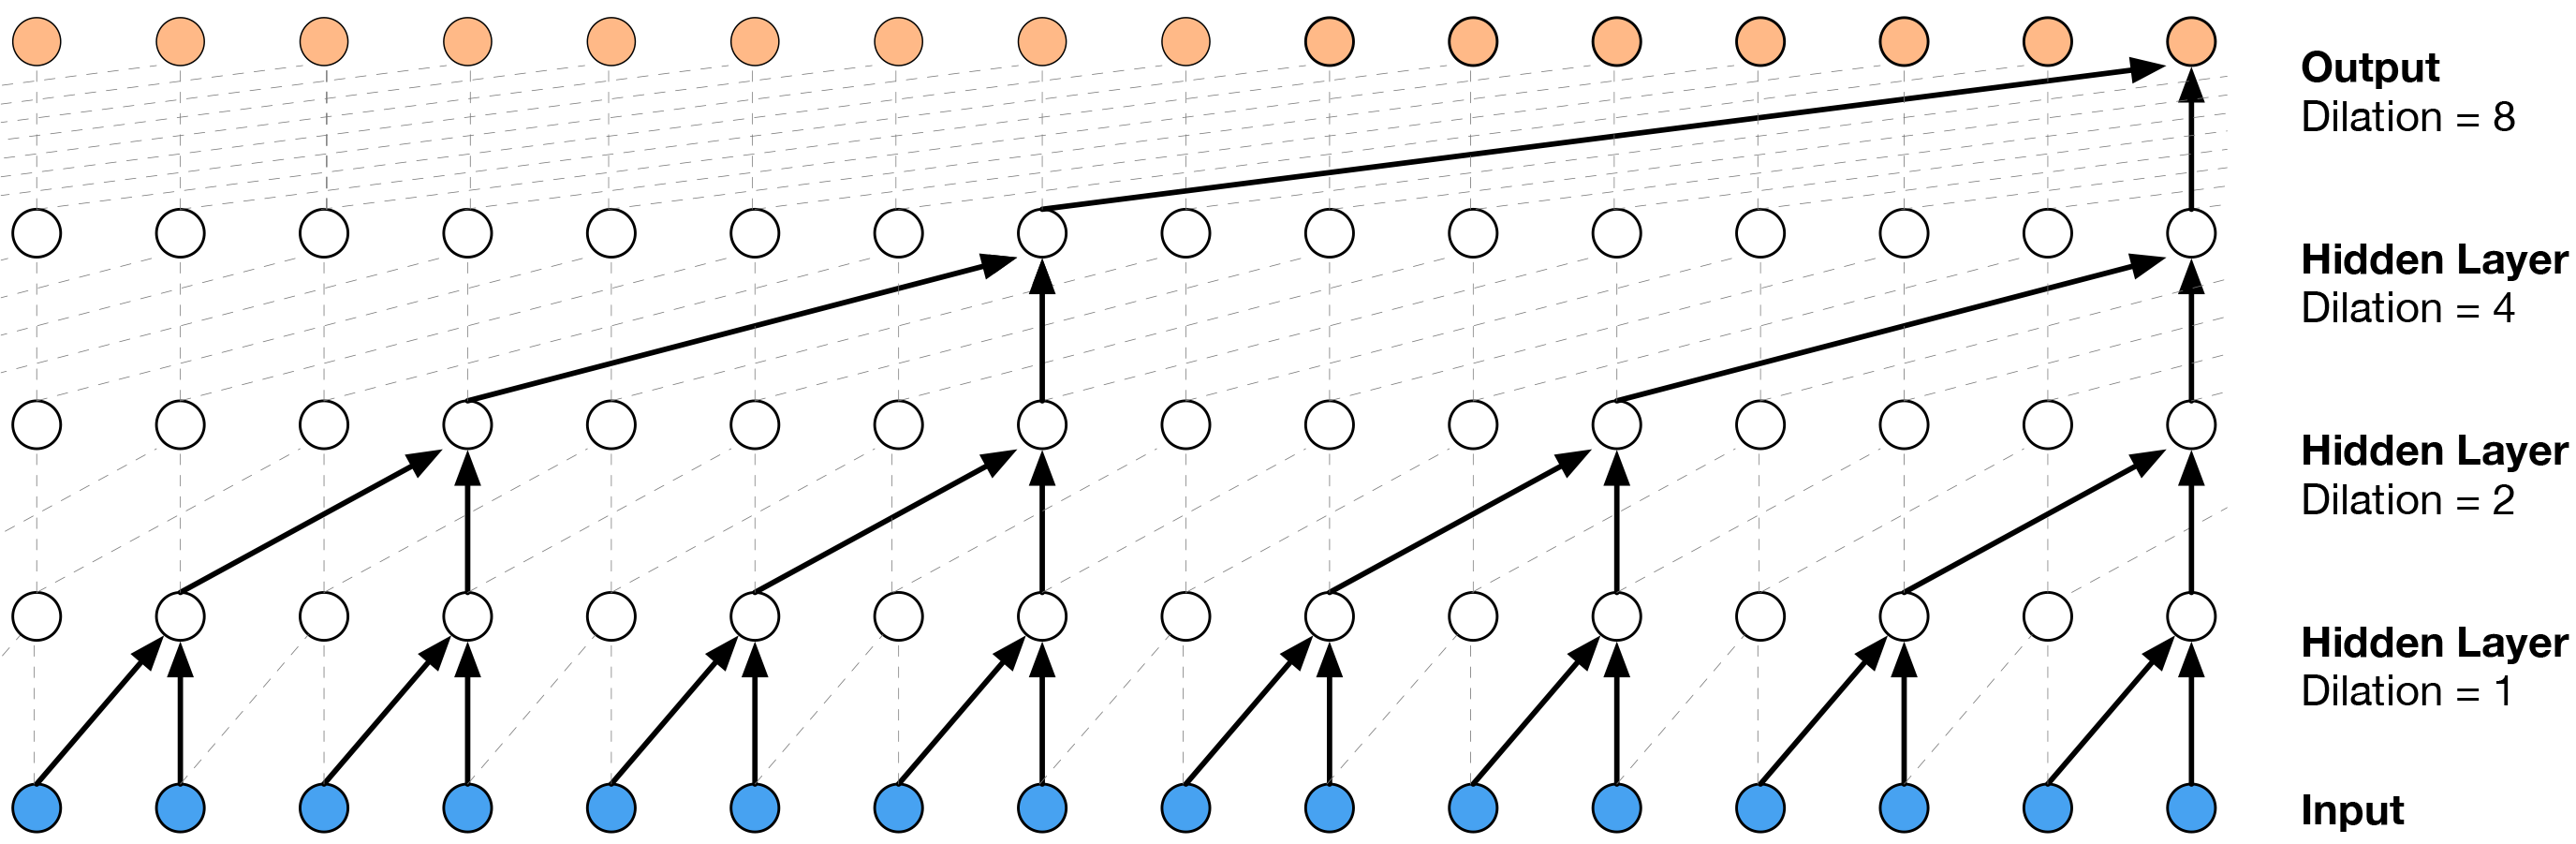
\includegraphics[width=1\linewidth]{wavenet.png}}
	\caption{Stacked dilated convolutional layers have a larger receptive field than normal convolutional layers. Image from Oord~et~al.~\cite{wavenet}.}
	\label{wavenet}
	\vspace{-0.5em}
\end{figure}

It is a fusion model consisting of two convolutional layers which feed into a number of LSTM layers. Short time spectral features from the 40 dimensional Mel-scale filterbank are input to both the convolutional and LSTM layers. The CLDNN based model shows a fair improvement over prior models; however, it is evident that the behaviour of these fusion architectures are not yet well understood. Individually, the behaviour of CNNs and LSTMs are difficult to interpret~\cite{cnnvis, visualisernn} and when combined their behaviour is more unpredictable.


\subsection{Automatic Feature Engineering for PD Diagnosis}

Our problem space is quite different from prior works in the field . Although mPower is the largest current dataset of PD data, its size is not comparable to computer vision and speech recognition datasets. For instance, the ImageNet~\cite{imagenet} dataset for computer vision consists of 14.2 million images and CLDNN~\cite{convlstm} was trained on 2,000 hours of speech. There are many (~30,000) walk recordings, but a majority of these are from a small subset of users. To avoid the `digital fingerprinting' effect\footnote{Neto et~al.~\cite{mpowerneto2017analysis} discovered that allowing mPower participants to appear in both train and test sets would result in an AUROC of 98 per cent for models trained on the walk sample. Stratifying by participant would reduce the AUROC to 45 per cent.} biasing the data, a maximum of 20 recordings were taken from any participant, resulting in a final dataset size of 12,000.

Overfitting was a major issue, and the problem changed from designing the most complex `deep' architecture capable of modelling the data, to designing an architecture which extracts useful features before severely overfitting. Simple, highly regularised models performed best in this task as they were less likely to memorise the data.


Accelerometer signals contain three dimensions of information $(x,y,z)$ and are sampled at a much lower rate: approximately 100$\,$Hz in the mPower data (vs. the 44,100$\,$Hz of audio). Experiments with various neural network architectures showed that using the normed acceleration signal performed better than using all three individual dimensions. Although using all dimensions provides more information, the lack of training data resulted in the neural architectures quickly overfitting before extracting useful features. 

Another difference is that diagnosing PD is a binary classification task and does not require intermediary predictions --- unlike Wavenet which was designed for speech generation, and CLDNN for speech recognition. There are also two distinct tasks (walking and balancing) involved in the mPower dataset, hence the final architecture would be an ensemble of at least two smaller architectures.


\begin{figure}[!htb]
	\centering\centerline{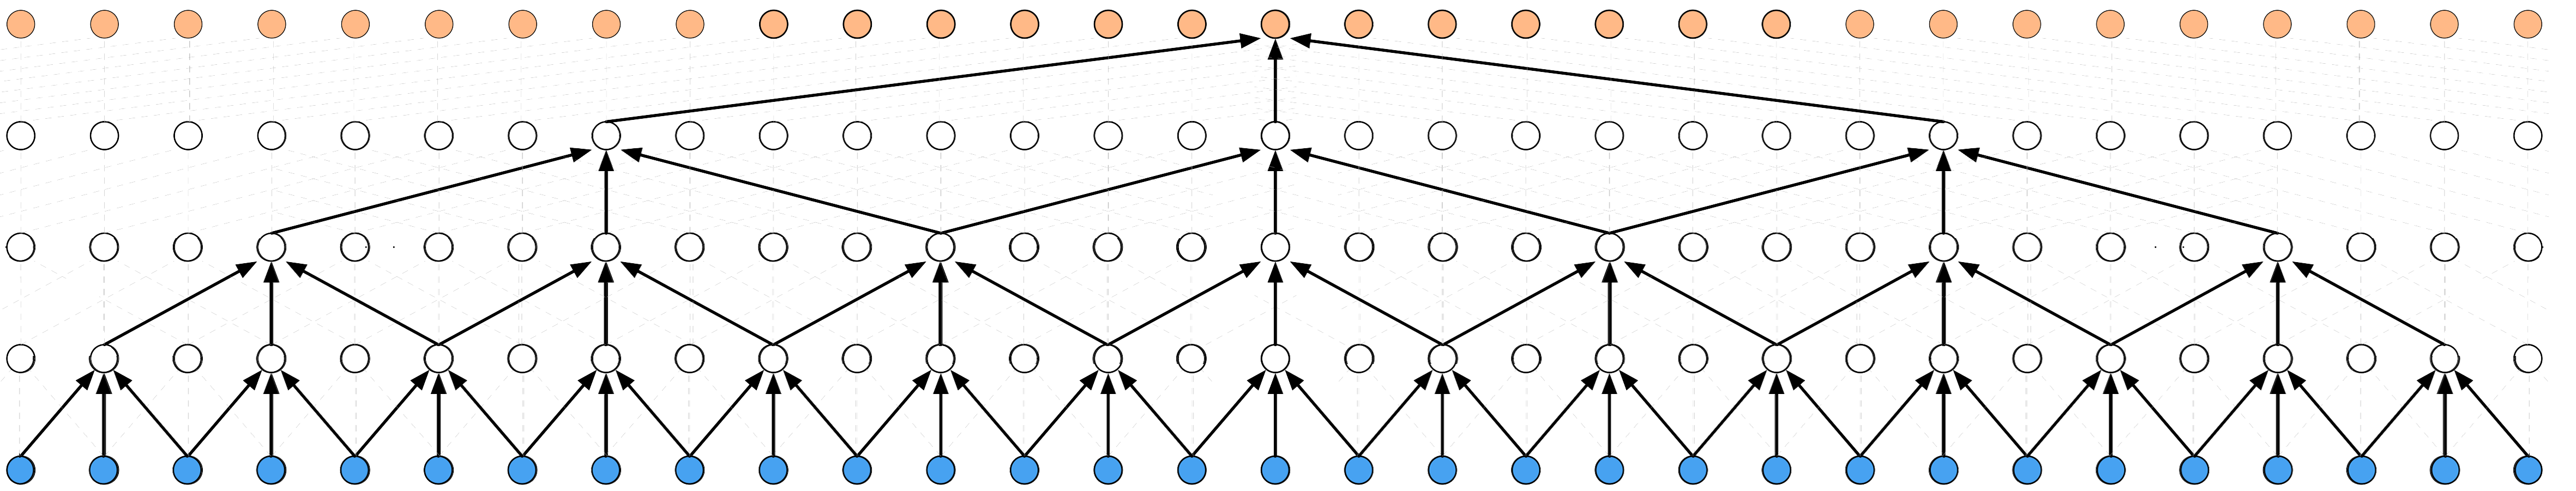
\includegraphics[width=1\linewidth]{biwavenet.png}}
	\caption{Bi-directional connections in Wavenet performed better in our task. }
	\label{biwavenet}
	\vspace{-0.5em}
\end{figure}

Out first architecture was inspired by Wavenet. As Wavenet is designed for speech generation, it only considers data from the `past'. We modified the Wavenet architecture, adding a dependency to `future' data. This was inspired by bidirectional RNNs which perform better in classification problems by utilising both past and future information. We term this \emph{Bi-Wavenet}, which exhibited improved convergence speed and peak validation accuracy compared to Wavenet. Following CLDNN, we explored a number of designs for the LSTM+CNN fusions. Layers of LSTMs followed by convolution layers seemed to be the most effective at extracting features. We denote this architecture \emph{LSTMConv}. 


Transforming the input data showed significant improvements to model performance. This is especially true with a limited amount of data, as models were less likely to overfit on the more interpretable data format. A short-time Fourier transform was used to map the input into the frequency domain. For the balancing data, a 3.2 second window with 1 second step length was the most effective input for both architectures. The walking data was more complicated as a long Fourier transform would remove valuable temporal information, and models trained on the raw signal would quickly overfit before extracting useful features. 

A compromise was made, training a model on both the raw and spectral signal with a 0.5 second window and 0.2 second step length. The outputs of each model were concatenated and a final neural network used to reduce the dimensionality of the data. Features were extracted by taking the activations of the penultimate layer of the network.


The LSTMConv architecture was vastly superior to Bi-Wavenet when handling spectral input. On the raw walking signal, Bi-Wavenet was noticeably more effective as LSTMConv based models would overfit on the walking signal before extracting useful features in validation. The final neural network architecture trained and used in the feature submission to the DREAM biomarker challenge is depicted in \hyperref[finalarchitecture]{Figure} \ref{finalarchitecture}.


\begin{figure}[!htb]
	\centering\centerline{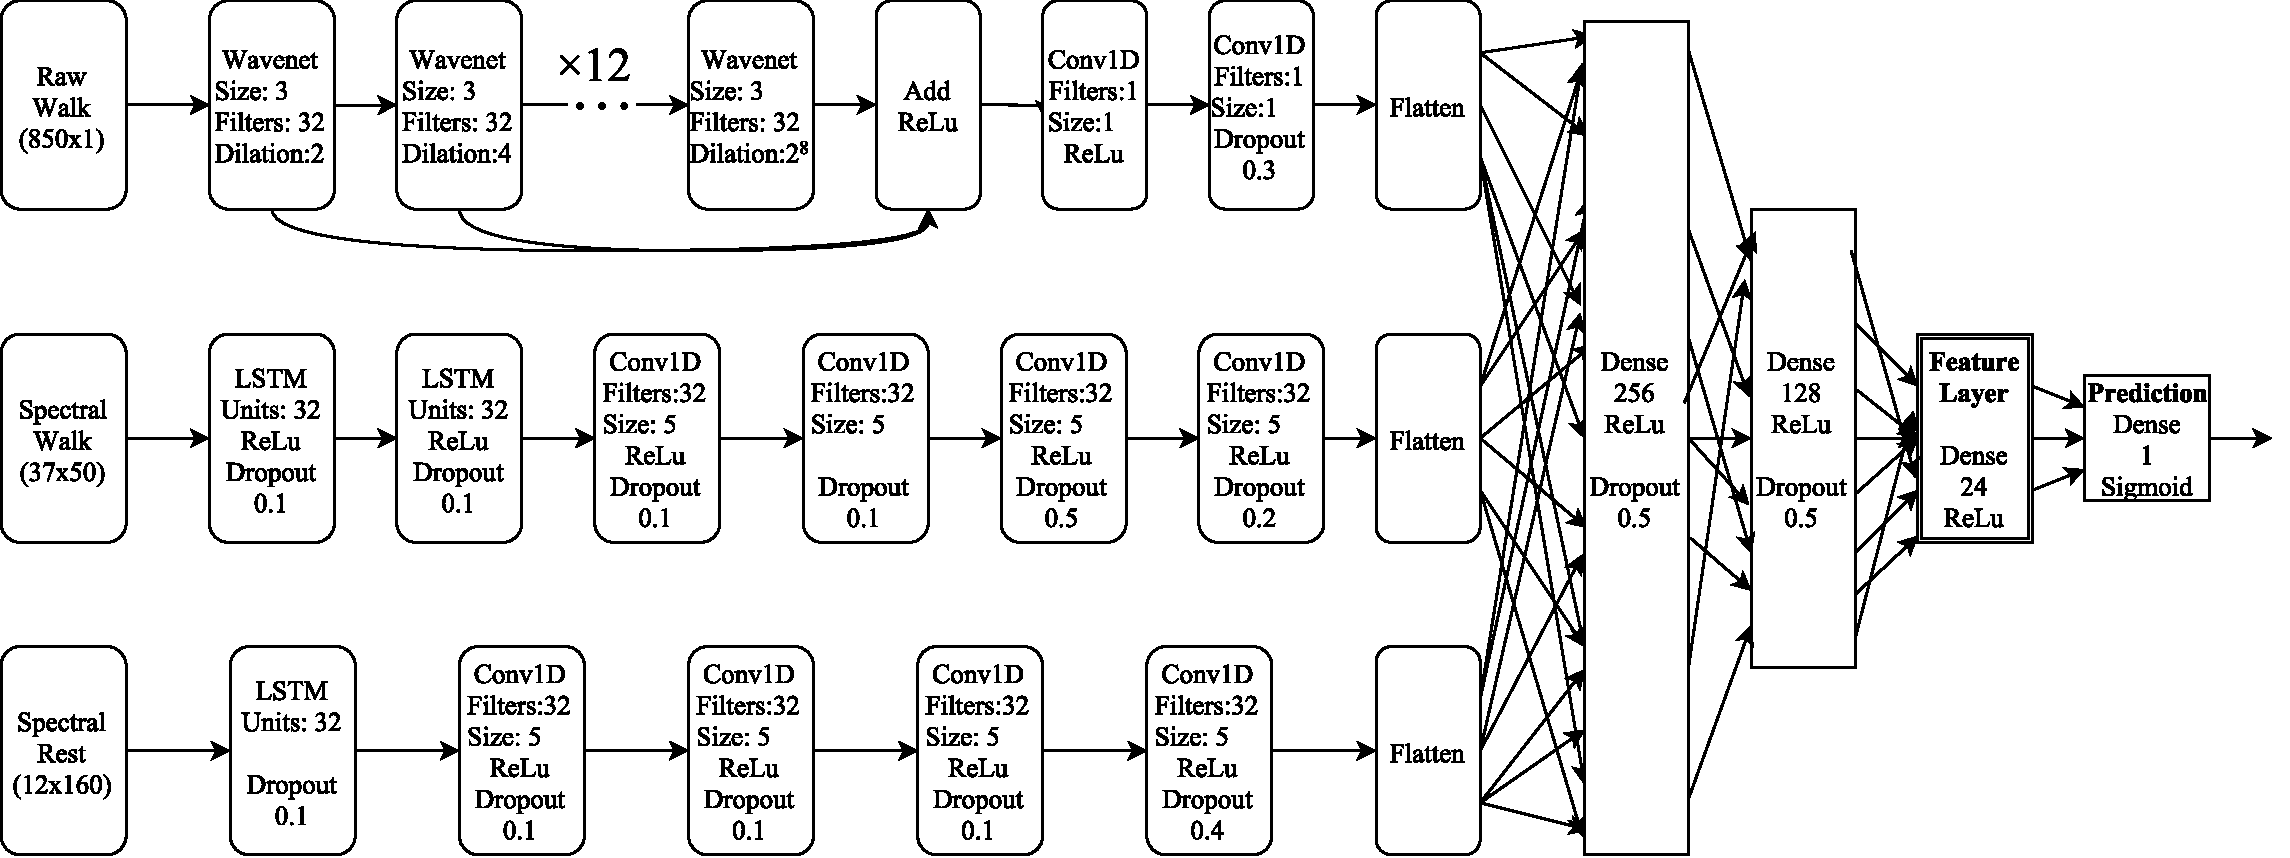
\includegraphics[width=1.2\linewidth]{final_architecture.pdf}}
	\caption{The final neural network architecture used to extract features submitted to the DREAM challenge.}
	\label{finalarchitecture}
\end{figure}


Using the DREAM evaluation methodology on the features we submitted, we obtained a cross validation AUROC of 71 per cent with all traditionally engineered features, and a cross validation AUROC of 80 per cent when the neural network based features were added. The results on the unseen testing dataset will be announced on the 31st of October at \url{synapse.org/digitalbiomarkerchallenge}. 



%ACCURACY WAS NOT A HUGE FOCUS AS TRAINING NEURAL NETWORKS IS STOCHASTIC AND THERE IS A LARGE VARIATION IN TRAINING PERFORMANCE DUE TO THE SMALL DATASET. THE ARCHITECTURES WE HAVE PROPOSED GENERALLY PERFORM WELL HOWEVER ARE NOT NECESSARILY BETTER THAN OTHERS.

%The purpose of this experiment was to investigate the feasibility of machine learning to 

%add noise and understand what happens -- what do the numbers represent, if anything?



%Computational power may have been too limited
%Due to the sensitivity of some features, it would be very interesting to extract all features on a short time scale and use a LSTM to observe
%however computational resources were too limited. 

\newpage
\section{Humans vs. Machines: A Discussion}
\label{powerml}
Now that we have shown the applicability of a range of techniques for diagnosing Parkinson's disease with raw sensor data, let us answer the question of what machine learning can provide to real-world diagnosis. The raw classifier performance on the mPower dataset is insufficient to replace neurologists; however, the results are impressive --- considering the diagnosis is solely based on a 4 second phonation of /aa/ with environmental noise, or a low quality accelerometer recording of walking.


\begin{highlight}
	Can machine learning differentiate between healthy individuals, and those with PD, but no speech difficulties?
\end{highlight}

In this section, we investigate if machine learning is able to detect symptoms imperceptible to a neurologist. Prior to training any models, we removed a set of participants with PD who declared themselves as having no speaking difficulties on the mPower UPDRS survey. We are aware that this relied on the honesty of participants and may not necessarily correlate to a neurologist's UPDRS assessment. There were 220/900 participants who had responded as having zero speaking difficulties and had filled in an answer other than the default (zero) for one other UPDRS criteria after the speech question. Of these participants, we listened to each audio sample and evaluated them for both quality and whether dysphonia was evident\footnote{Optimally, a neurologist would be involved in this process. The resources were not available. Note that the evaluator had listened to 1,600 speech samples from PD and control participants to develop the filtering criteria and is familiar with the characteristics of dysphonia.}. This resulted in a final set of 86 participants, which were removed from the dataset in all earlier models prevent overfitting from model tweaking. 


\begin{table}[!htb]
	\caption{Results of the FWLS ensemble on the 86 unseen PD participants with no speaking difficulties and the 28 PD participants in Sakar~et~al.~\cite{sakar2012}. Data augmentation was not applied due to limited /aa/ phonation time in recordings from Sakar~et~al.}
	\label{machvshumanresult}
	\centering
	\begin{tabular}{@{}rcccc@{}}
		&  \specialcell{Cross\\Validation} & \specialcell{No Speech\\Difficulties} & \specialcell{\\Sakar} \\ \midrule
		Accuracy [\%]    &  $75.4\pm2.7$ & $73.1\pm1.9$ &$85.7$\\ \midrule
		Sensitivity [\%] &  $71.1\pm4.1$ & $73.1\pm1.9$ &$85.7$\\ \midrule
		Specificity [\%] &  $79.7\pm4.6$ & $-$ &$-$   \\ \midrule
		AUROC [\%]       &  $82.5\pm2.6$ & $78.3\pm1.7$ &$90.6$ \\ \midrule
		Total Subjects & 1716 & 86 & 28 \\ \midrule 
	\end{tabular}
\vspace{-0.5em}
\end{table}


We applied the most powerful model we had available, the FWLS ensemble (\textit{\hyperref[spensemble]{Section}} \ref{spensemble}) to this task with our standard ten times repeated 10-fold cross validation. The set of 86 participants were divided into ten groups of 8-9 individuals, and the ensemble trained on all except one of these groups. To confirm results and ensure that the models able to generalise outside of the mPower dataset, we test our model's performance on the speech samples of 28 subjects with PD released by Sakar~et~al.~\cite{sakar2012} on the UCI Machine Learning repository. The best /aa/ phonation for each participant of 1.5 seconds of length was extracted as testing data. The results are presented in \textit{\hyperref[machvshumanresult]{Table}} \ref{machvshumanresult}. 



\vspace{-0.1em}
\begin{highlight}
	Machine learning is able to diagnose participants with PD without speech difficulties.
\end{highlight}
\vspace{-0.2em}
Surprisingly, there is no statistically significant difference between the specificity when diagnosing participants with perceptible and imperceptible dysphonia. This implies that there must exist some features, or a combination of features which enable the models to distinguish participants with PD and no speech difficulties and control. Some of these features will be explored in the next section. The result on Sakar~et~al.~\cite{sakar2012} provides strong evidence that the mPower trained models are not overfitting, and generalise well to unseen data. 


\vspace{-0.2em}
\subsection{Human Hearing vs. Signal Processing}
\vspace{-0.1em}
\label{formalfeatures}
As the ensemble model obtains similar classification accuracies on both the participants with and without perceptible speech difficulties, combinations of features must exist which distinguish Parkinsonian and normal speech. Some features quantify a characteristic which should be discernible with human hearing, whereas others may measure more abstract qualities. 

\vspace{-0.1em}
\begin{highlight}
	There must be a subset of features which differentiates participants with PD and no speech difficulties to healthy individuals.	
\end{highlight}

\vspace{-0.2em}

We investigate how some of the features we have introduced relate to human senses. If individuals with PD and and \textit{no speech difficulties} (NSD)\footnote{In this section, \emph{NSD} denotes the set of participants with Parkinson's disease and no speech difficulties and \emph{PD} denotes the set of participants with Parkinson's disease and speech difficulties.} are distributed similarly, and NSD and control differently, this implies that the feature is likely \emph{inaudible} to the human ear. If the distributions of NSD and control are similar and control and PD different, the feature is likely to be \emph{audible}. Otherwise, the distribution of NSD may be similar to neither PD nor control. This may imply that the feature is audible to the human ear; however, not directly associated with Parkinson's disease. 


These hypothesis will be tested with two approaches. As the features are generally not distributed in a Gaussian fashion, we employ the non-parametric Kruskal-Wallis~\cite{kruskal1952use} ANOVA test, using the Dwass-Steel-Critchtlow-Flinger method to control for repeated pairwise comparisons~\cite{DCSF}. Two groups are considered sampled from different distributions if $p<0.05$, denoted with a star\textsuperscript{*} and $p<0.001$ denoted by three stars\textsuperscript{***}. 

We are also interested in the result that two distributions are similar; however, the assumptions underlying $p$-value hypothesis testing only allow us to conclude that there is insufficient evidence to show the distributions are different~\cite{fisher1937design}. Bayesian tests such as the Bayes factor ANOVA test can quantify evidence in support of two distribution means being the same (the null hypothesis)~\cite{bayesianttests}. However, these tests are parametric, requiring a prior assumption over the distributions. We apply the Aligned Rank Transform~\cite{artool} to transform the data into a format suitable for Bayes factor analysis. Two distribution means are considered similar if $p>0.25$ and $BF<\frac{1}{3}$, denoted by a dagger\textsuperscript{†}. The Aligned Rank Transform is less suitable when repeated comparisons are performed~\cite{fan2017rank}, hence the Kruskal-Wallis test is preferred when testing for differences in the distribution (rejecting the null hypothesis).

Note that the results presented in this section are influenced by selection bias, as the NSD group have been verified as performing the task properly. The other groups may have more outliers from performing the task incorrectly or excessive background noise. This should be considered when interpreting conclusions --- `bad' samples often appear as outliers, but this may not be the case for all features.


\begin{figure}[!htb]
	\centerline{
		\begin{subfigure}[]{0.52\textwidth}
			\label{f0boxplot}
			\caption{Standard Deviation of $f_0$ ($>4.0$ removed)}
			\centering
			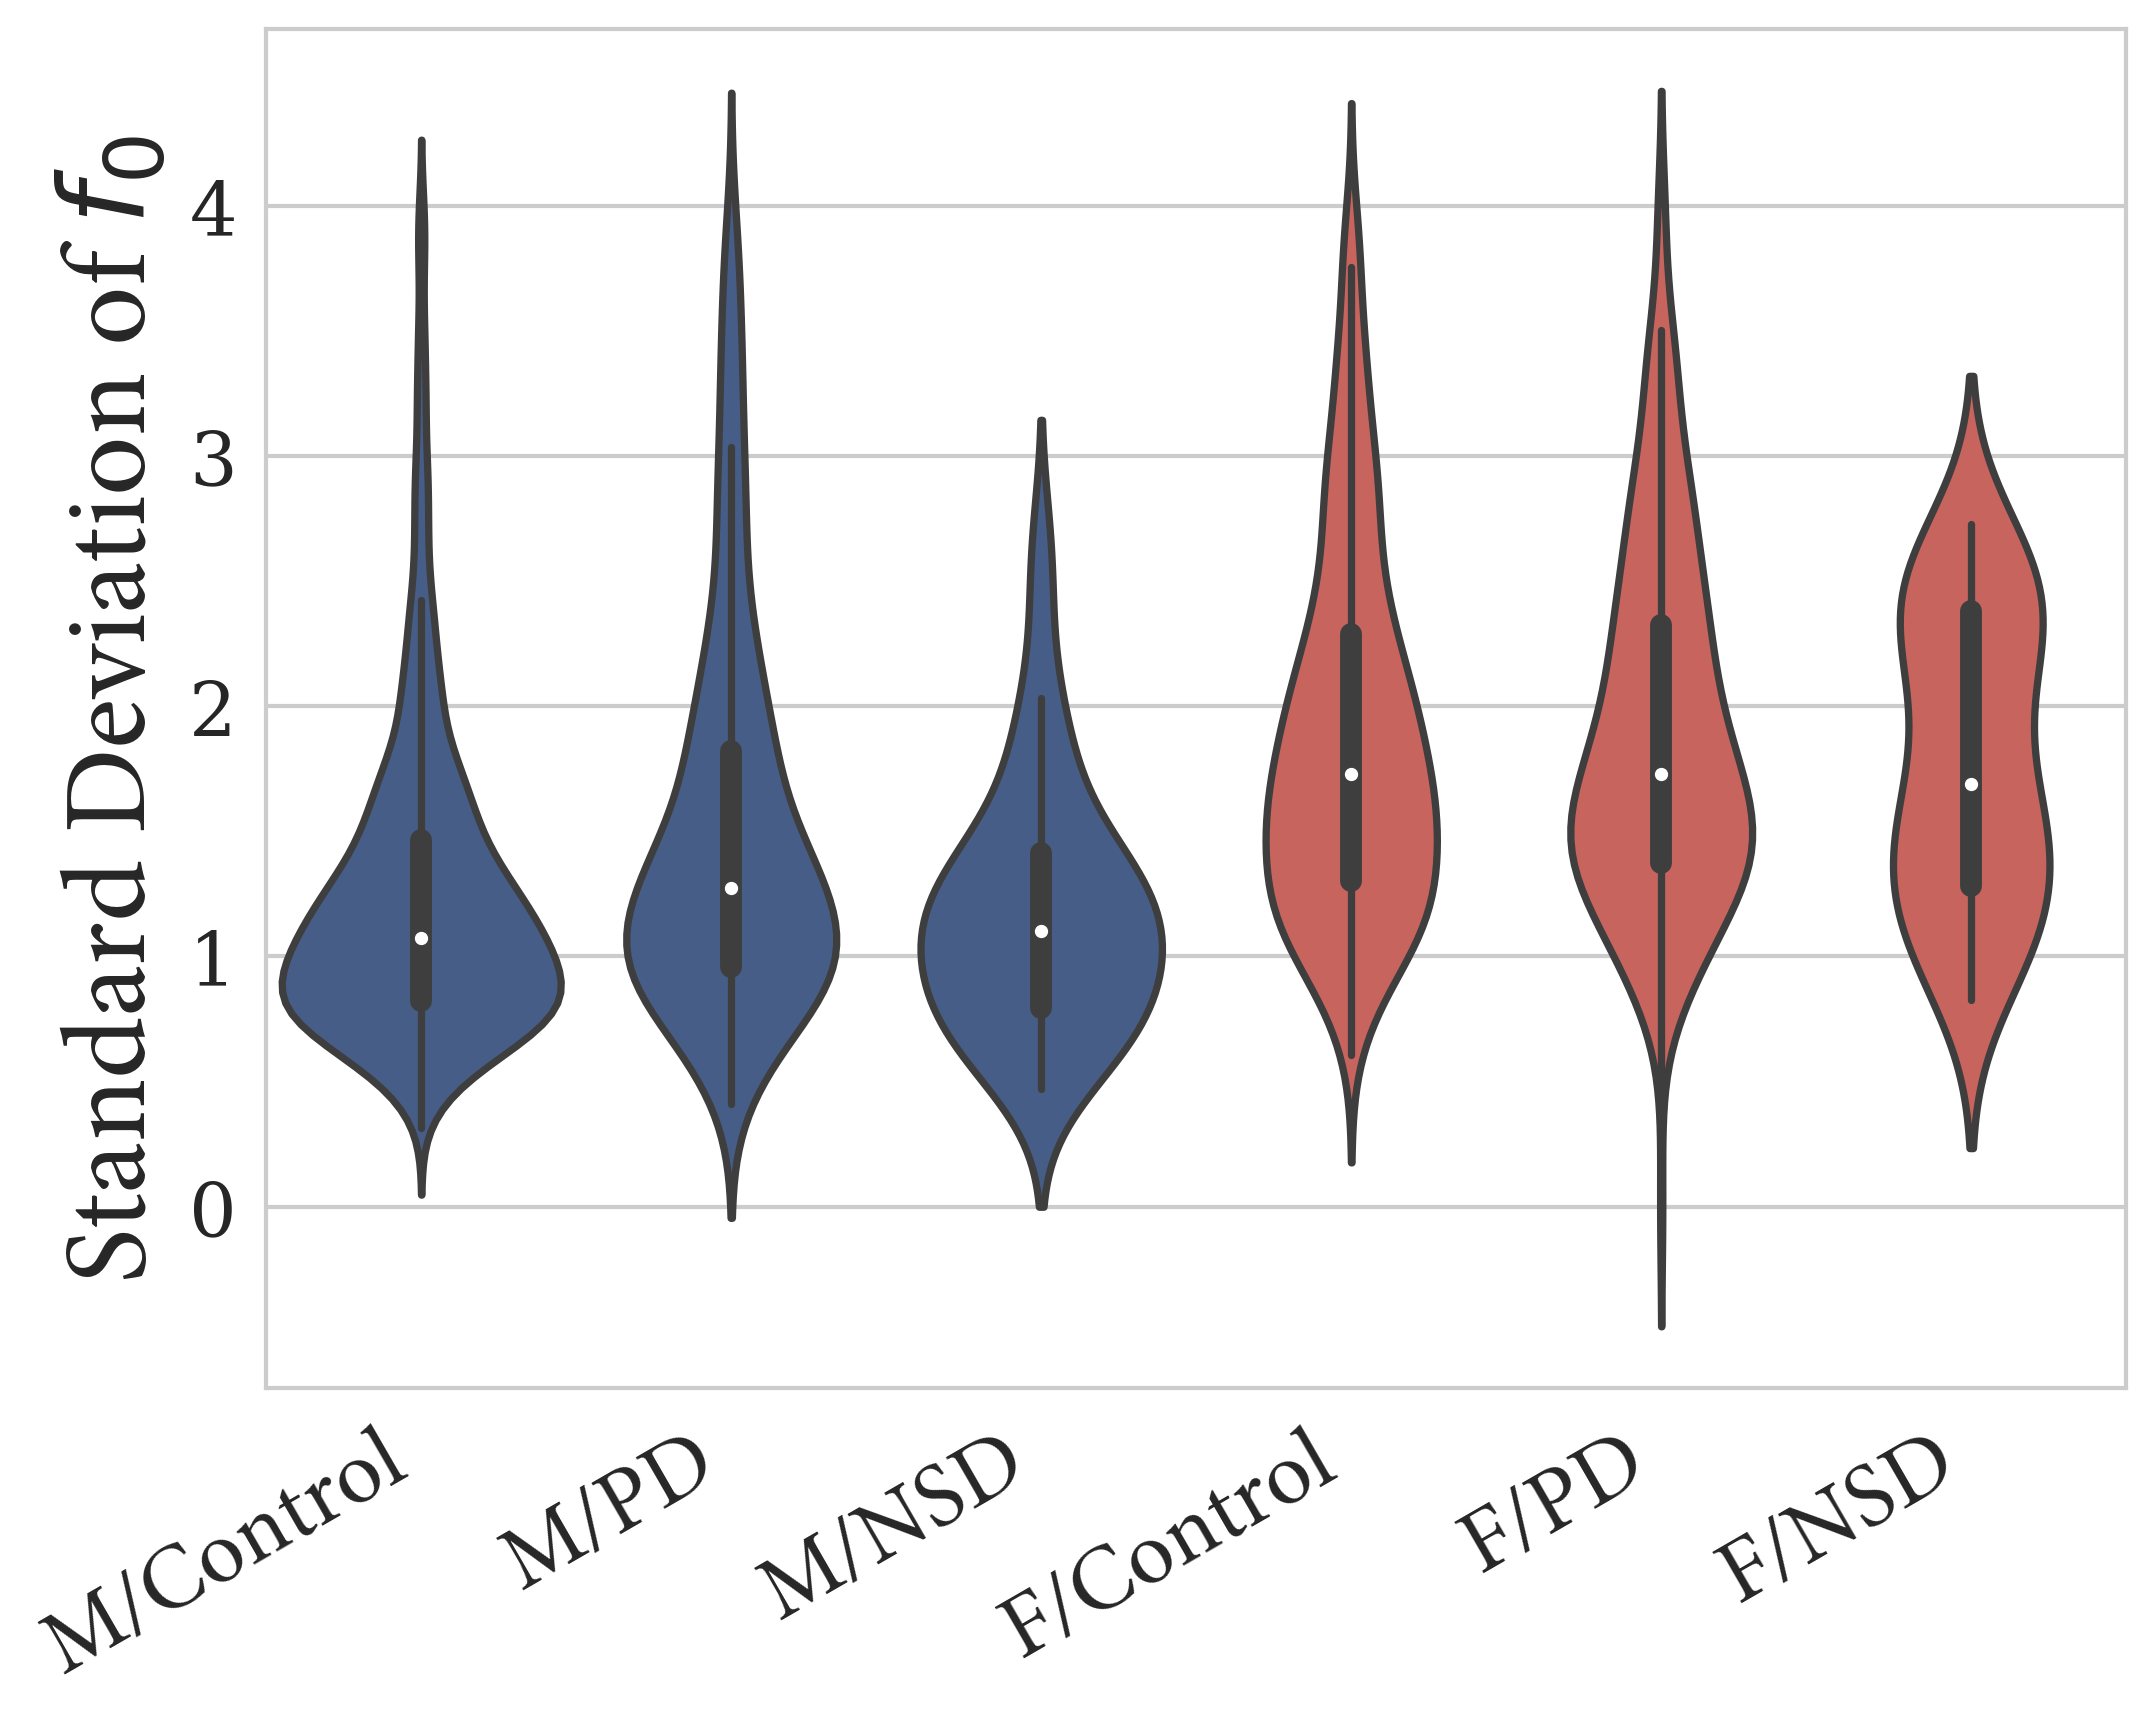
\includegraphics[width=0.96\linewidth]{stdevf0_boxplot.png}
		\end{subfigure}%
		\begin{subfigure}[]{0.52\textwidth}
			\label{vferboxplot}
			\caption{Vocal Fold Excitation Ratio ($>0.005$ removed)}
			\centering
			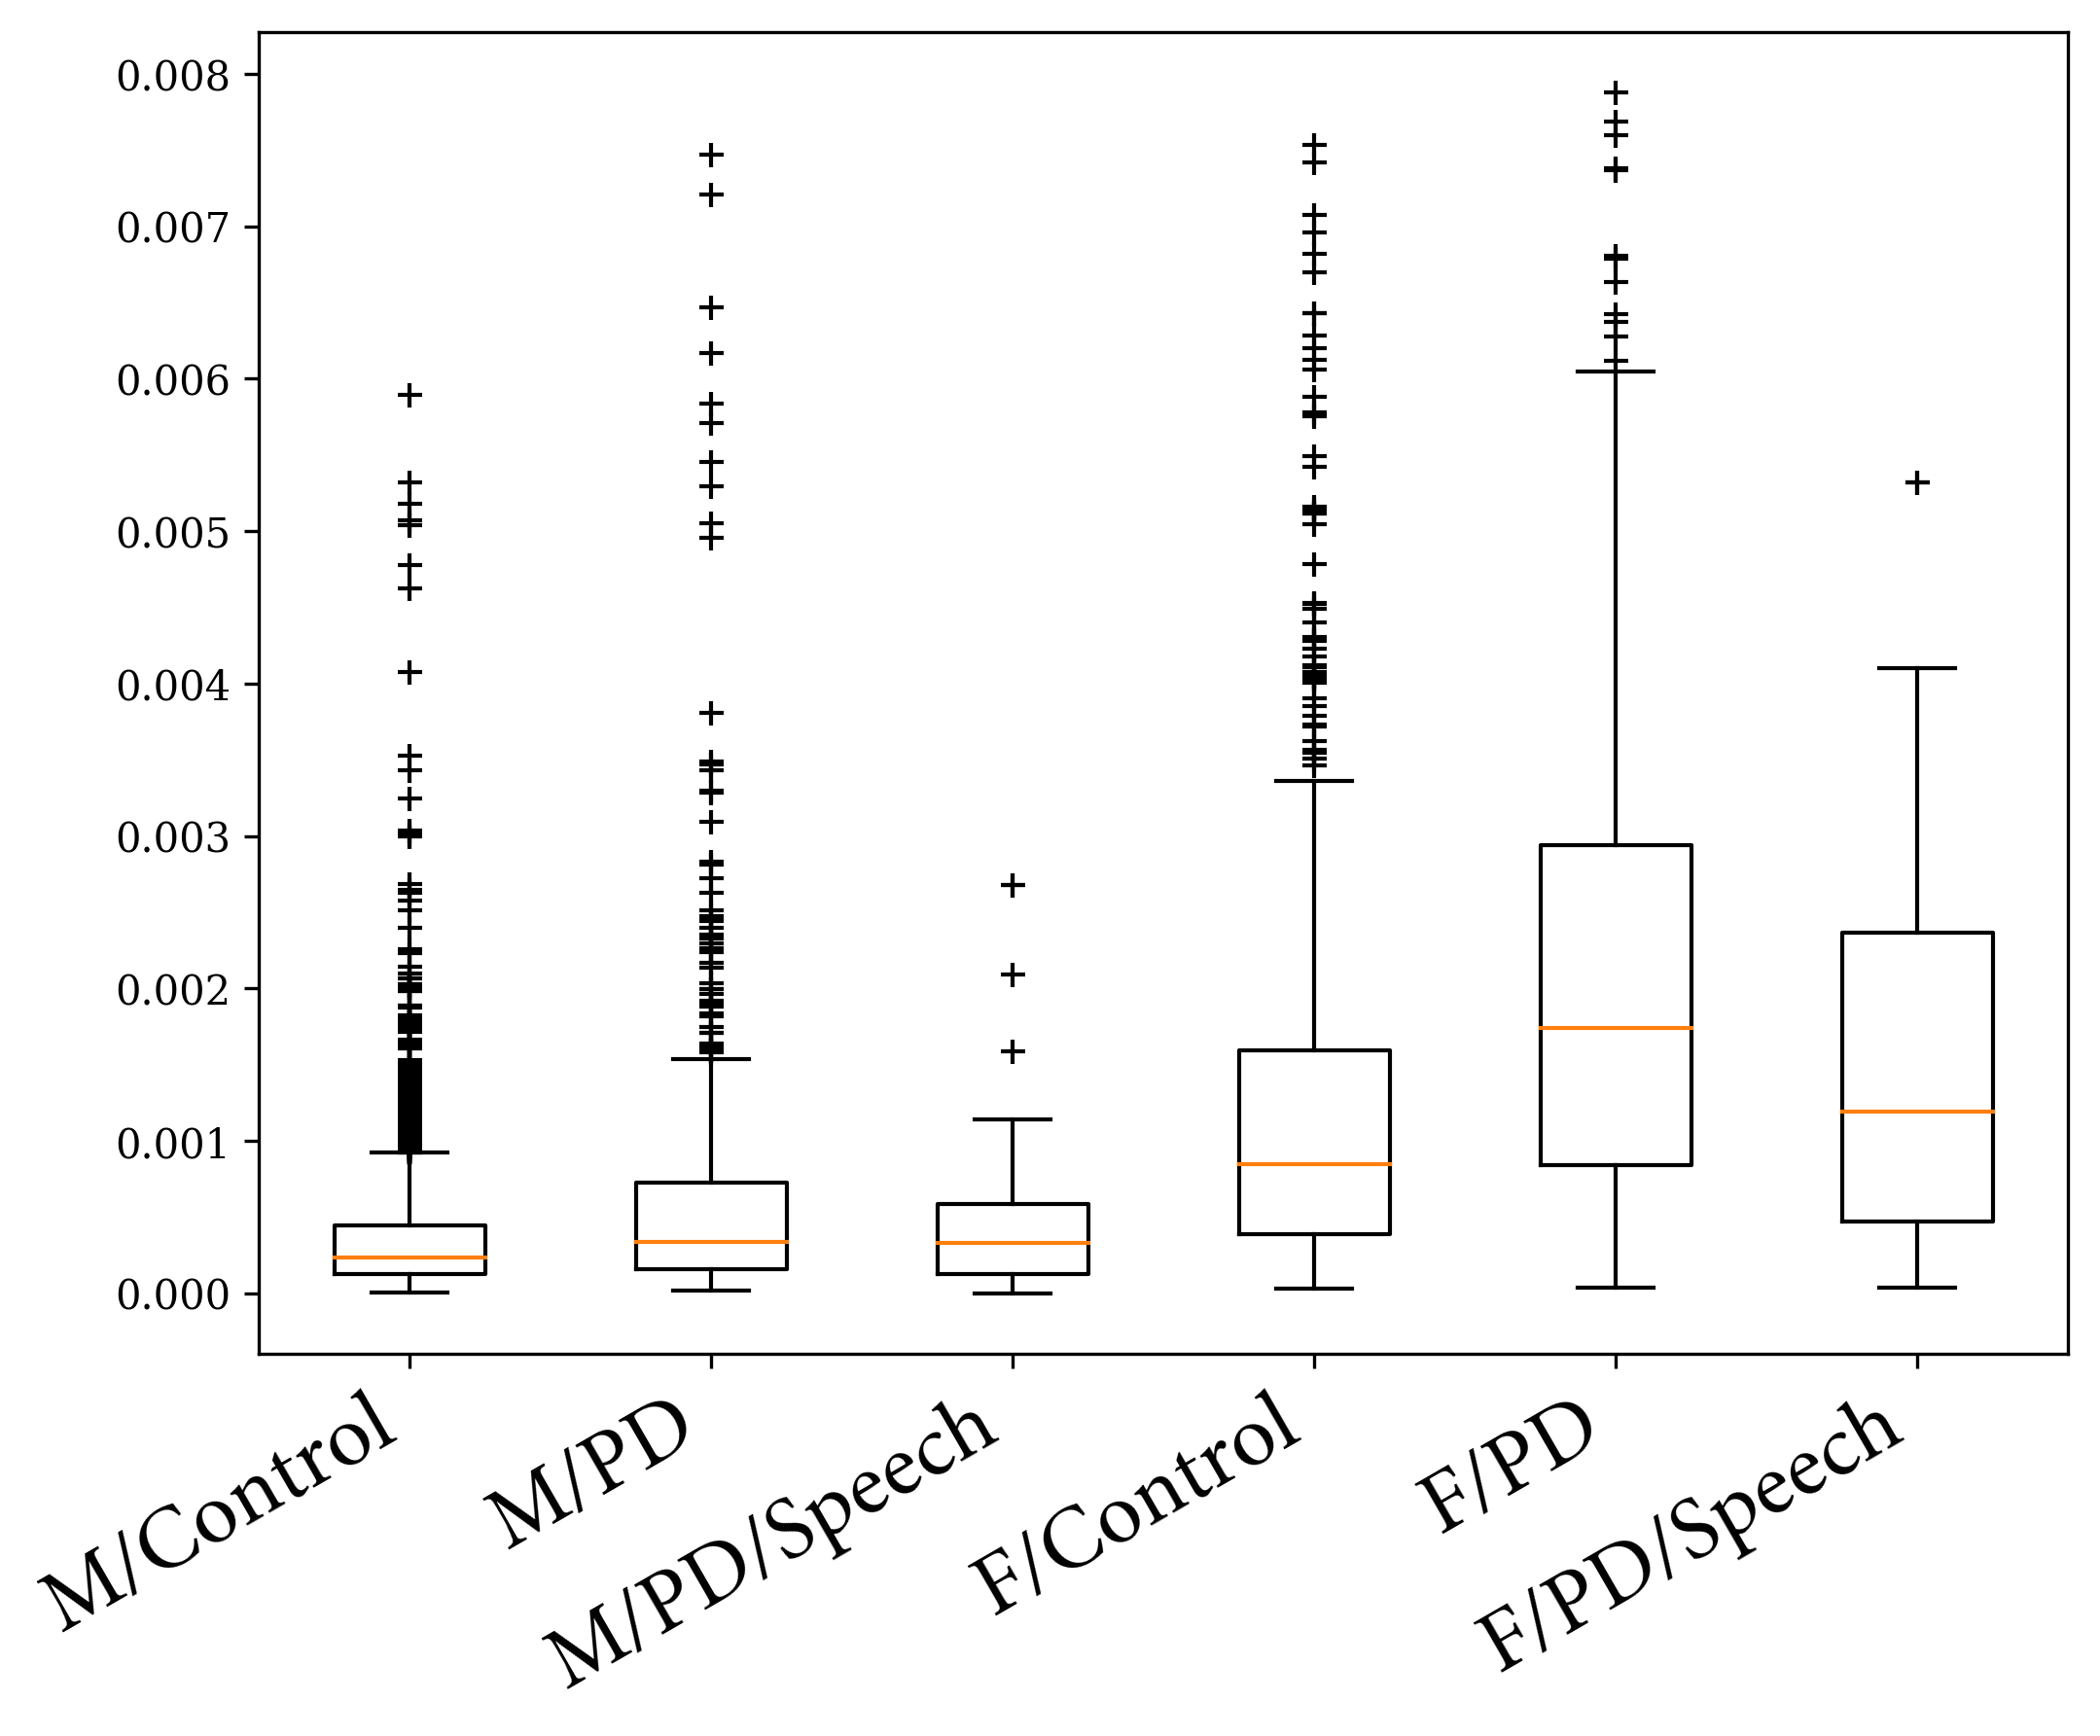
\includegraphics[width=0.96\linewidth]{VFER_boxplot.png}
		\end{subfigure}
	}
	\caption{Violin plots of features over all samples used in the machine learning models with extreme outliers removed. (a) Standard deviation of $f_0$ in males is likely audible to the human ear as control and NSD are distributed similarly \textsuperscript{†}, whereas control and PD are different\textsuperscript{***}. There is no significant variance in $f_0$ between females\textsuperscript{†}. (b) The VFER of female speech is likely audible to humans as control and NSD have similar  distributions\textsuperscript{†} while control and PD are different\textsuperscript{***}. Additional data is required for males.}
	\label{f0vferboxplot}
\end{figure}

The human ear is sensitive to changes in pitch, and Parkinsonian speech has greater fluctuations in frequency. Therefore it is expected that the NSD group has a lesser standard deviation of $f_0$ than the PD. The amount of noise (related to breathiness) should also be perceivable with human hearing. This feature is quantified by the harmonics to noise ratio (HNR); however, the HNR was not a feature strong enough to differentiate normal and dysphonic speech; thus, the Vocal Fold Excitation Ratio, an extension of the HNR was used instead~\cite{spoverview}. The differences between PD participants with and without speech difficulties are presented in \textit{\hyperref[f0vferboxplot]{Figure}} \ref{f0vferboxplot}. 

%F0
%500608114325 4.778964 0.2064219
%0.09593154 0.7069853 0.5478061

%VFER
%8.285428e+21 0.2937744 0.753058
%568957670 0.5045708 0.3774322



Based on the evidence in \textit{\hyperref[f0vferboxplot]{Figure}} \ref{f0vferboxplot}, we can conclude that there is substantial evidence the variations in $f_0$ in males are audible to humans. The $f_0$ is estimated with the SWIPE algorithm~\cite{camacho2007swipe} and it is possible that the shorter pitch periods of female phonation cause a larger error margin in the $f_0$ estimates~\cite{f0estimation}, blurring the difference between dysphonic and normal female phonation. The evidence that VFER is audible to humans is less substantial, but it is not a strong measure for differentiating control and NSD groups.

\begin{highlight}
	Features such as the standard deviation in the fundamental frequency and the signal to noise ratio are not useful at distinguishing individuals with invisible PD symptoms.
\end{highlight}


\begin{figure}[!htb]
	\centerline{
		\begin{subfigure}[]{0.52\textwidth}
			\label{dfaboxplot}
			\caption{Detrended Fluctuation Analysis}
			\centering
			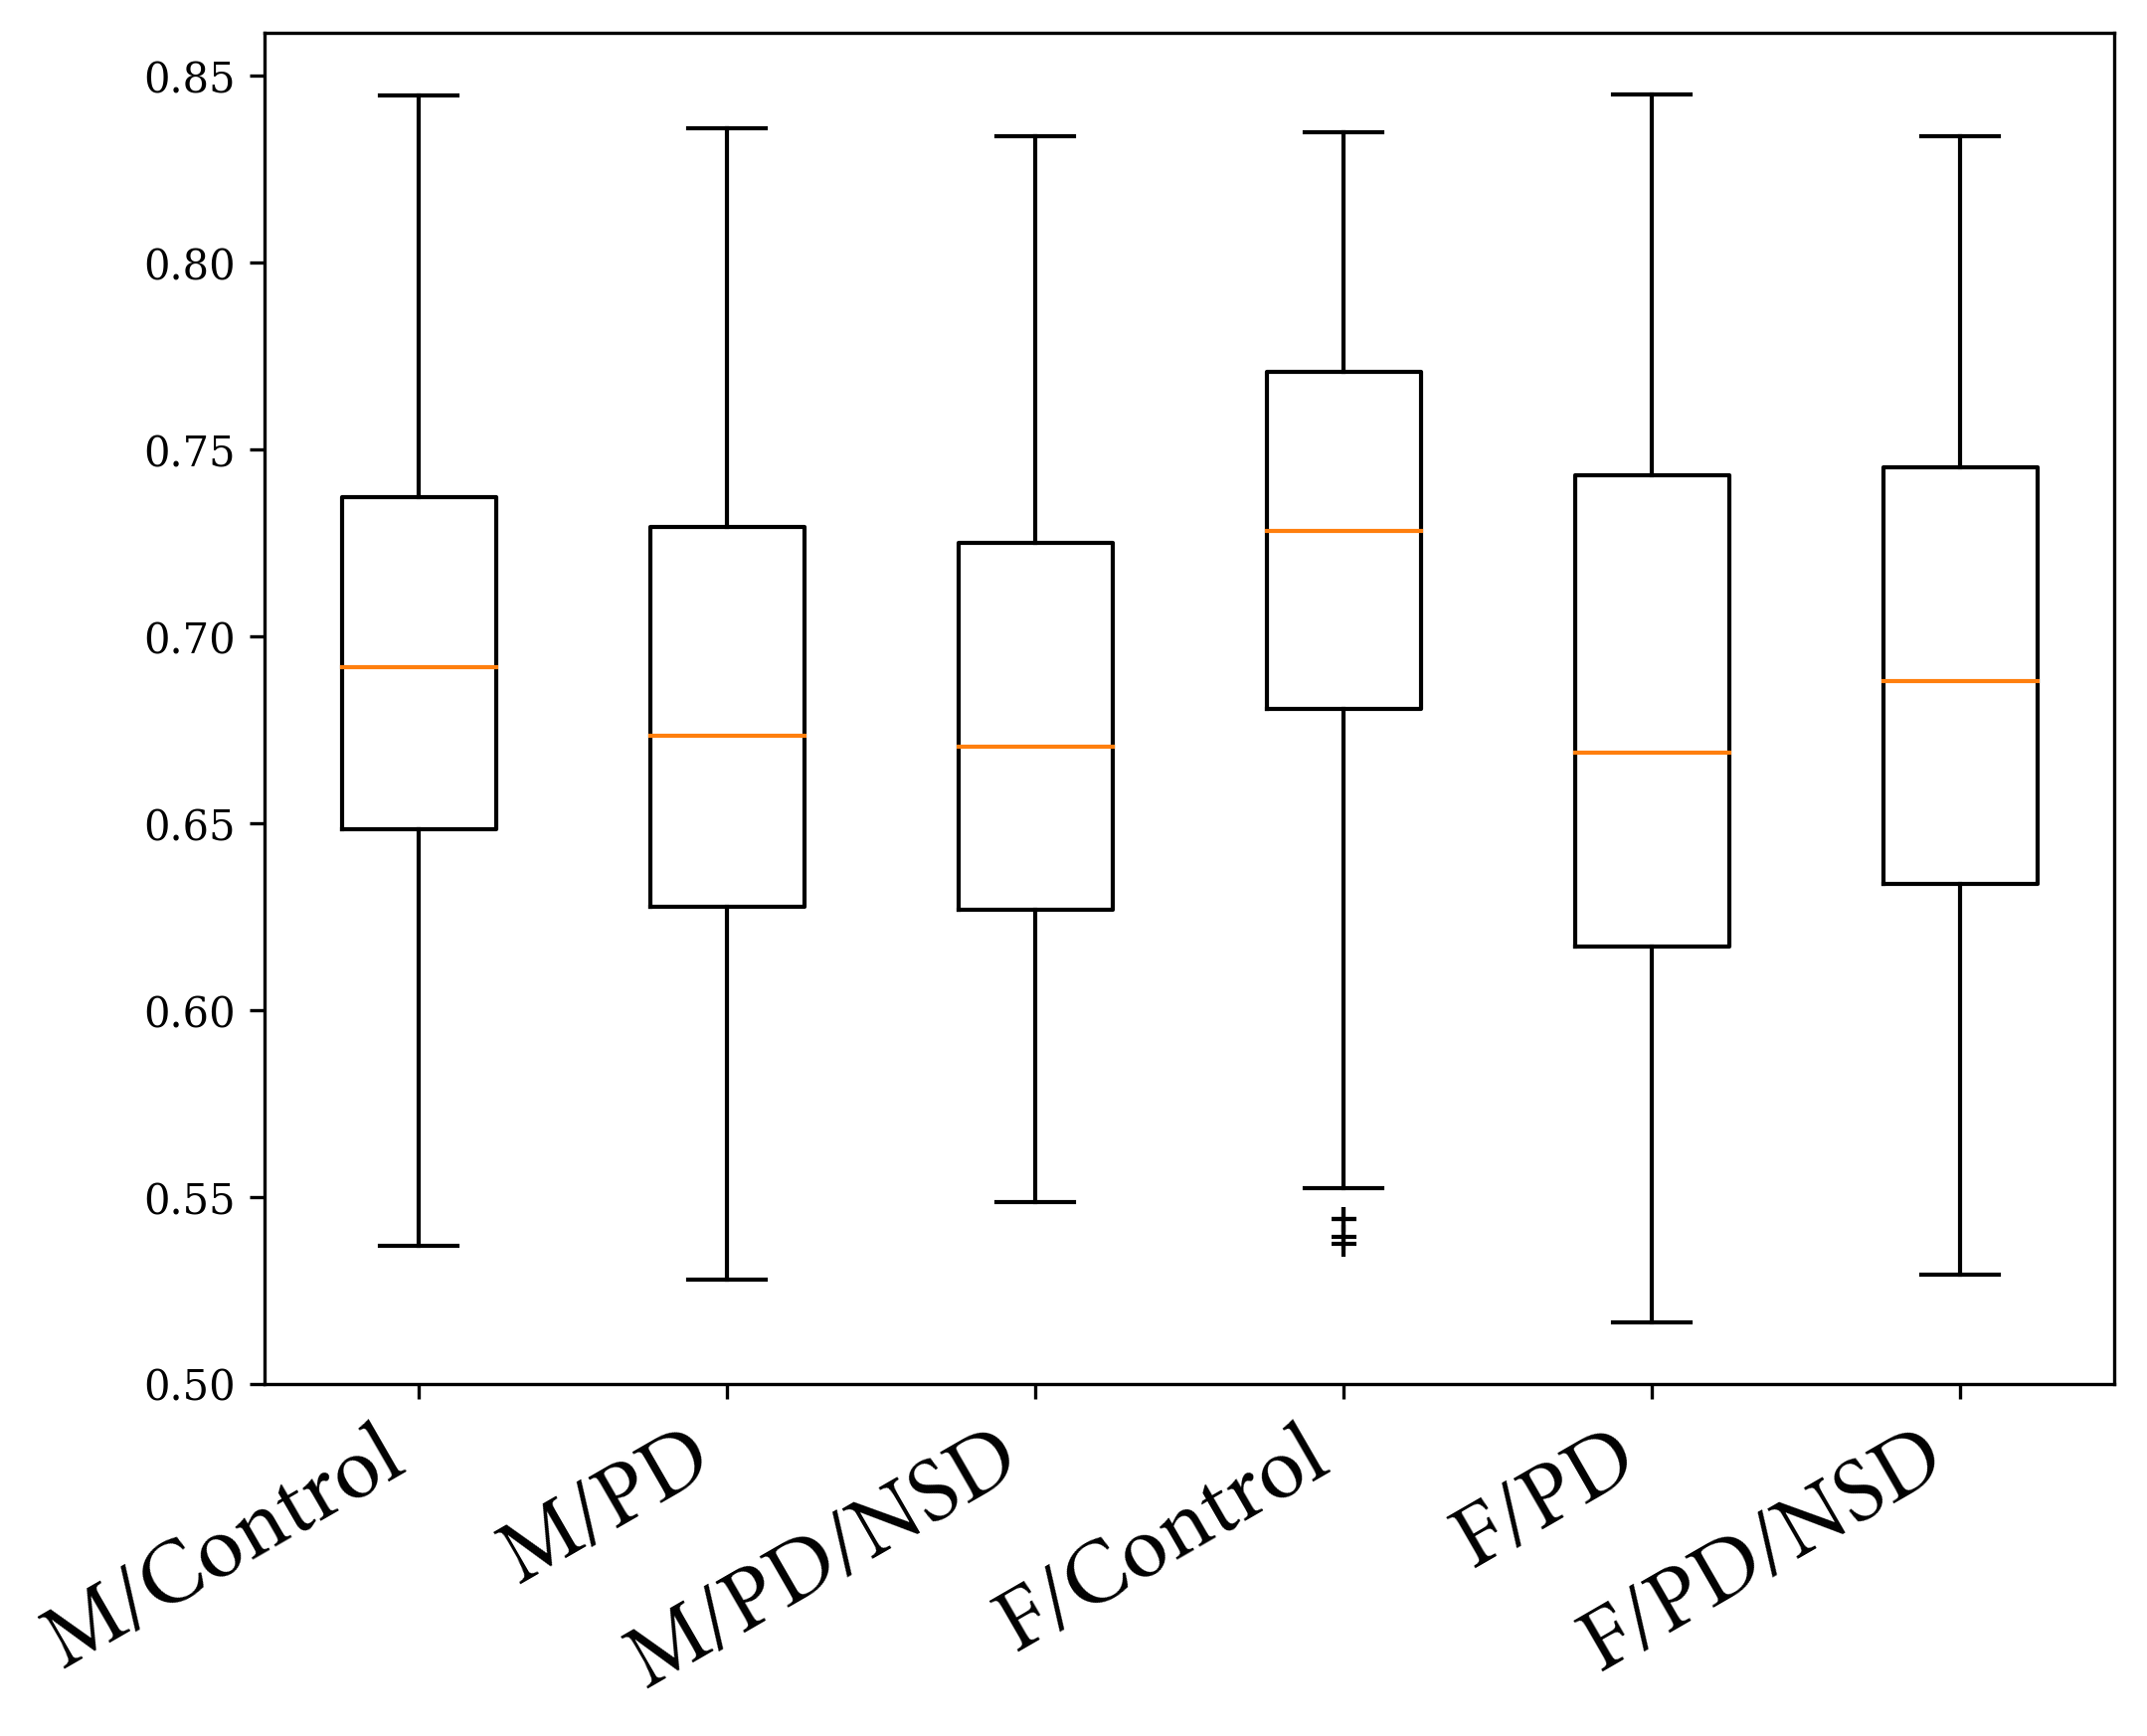
\includegraphics[width=0.96\linewidth]{DFA_boxplot.png}
		\end{subfigure}%
		\begin{subfigure}[]{0.52\textwidth}
			\label{rpdeboxplot}
			\caption{Recurrence Period Density Estimation}
			\centering
			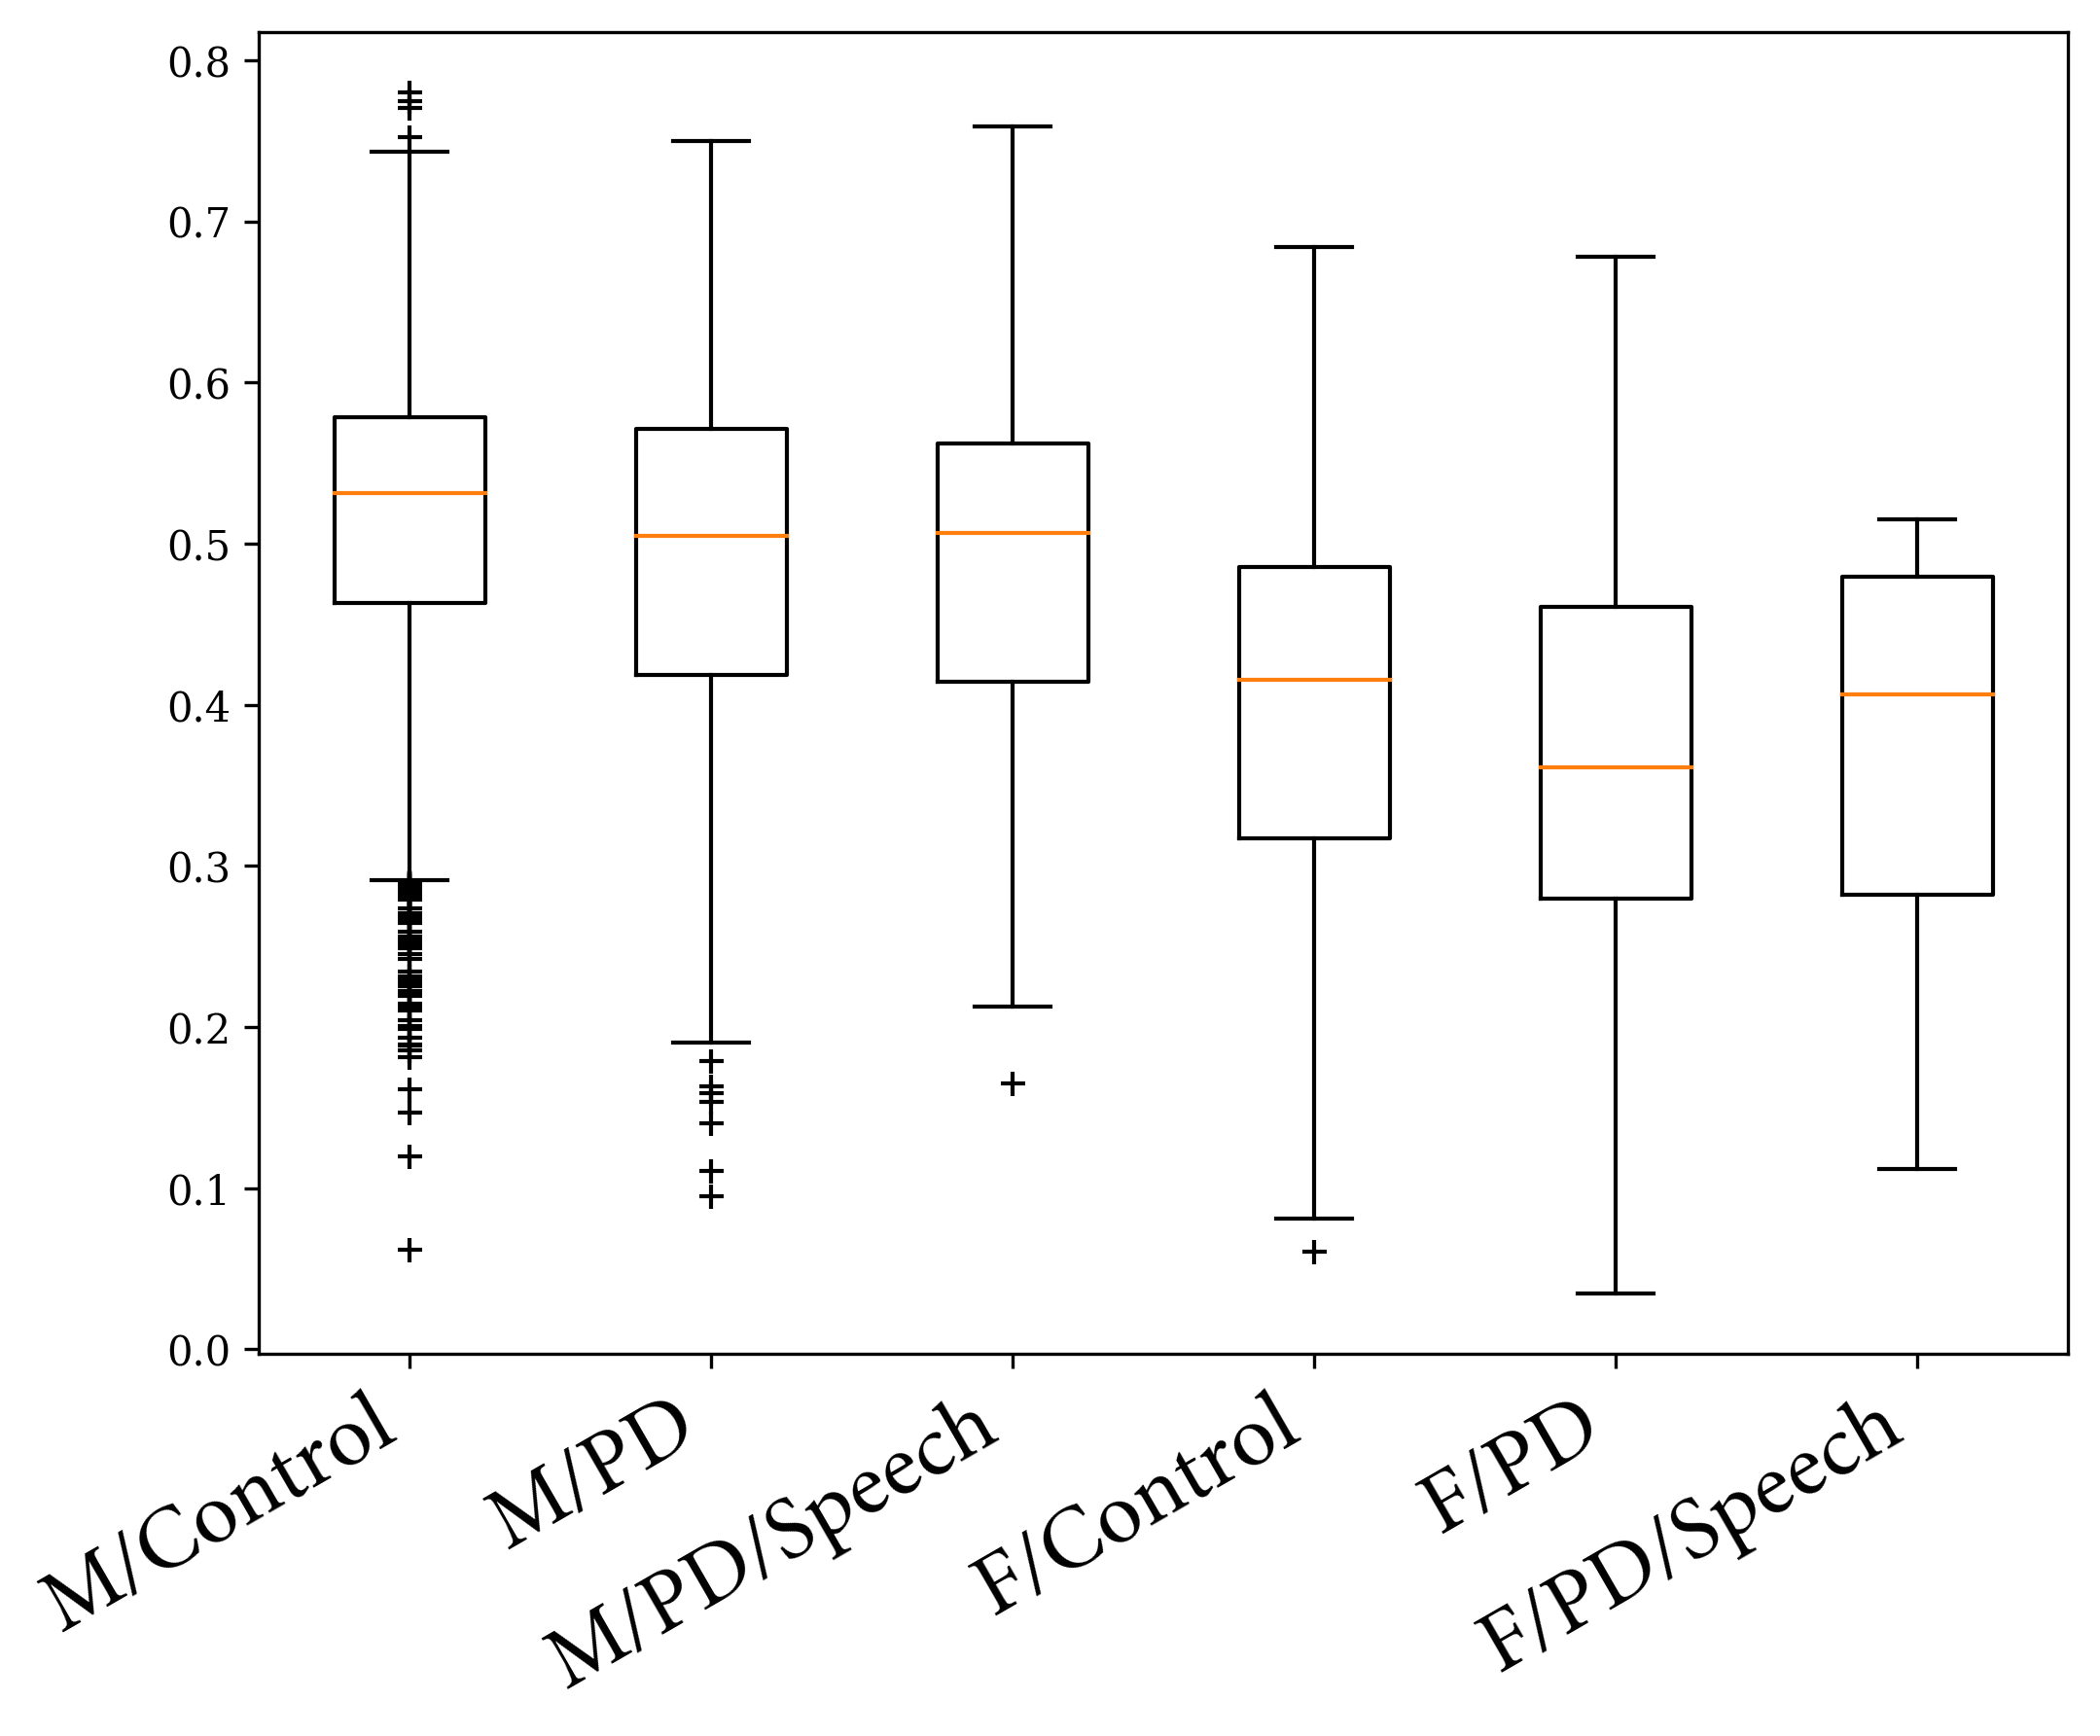
\includegraphics[width=0.96\linewidth]{RPDE_boxplot.png}
		\end{subfigure}
	}
	\caption{(a) DFA is likely inaudible in both males and females as PD and NSD are distributed similarly\textsuperscript{†} and control and NSD differently\textsuperscript{*}. (b) RPDE likely isn't audible in males as PD and NSD are distributed similarly\textsuperscript{†} and control and NSD differently\textsuperscript{*}. For females, evidence in insufficient to conclude whether NSD is sampled from a different distribution to control or PD.}
	\label{dfarpdeboxplot}
\end{figure}

DFA and RPDE are two of the stronger non-linear measures used in prior work, which detect Parkinsonian dysphonia~\cite{splittledysphonia2009}. DFA is a measure of the autocorrelation of a signal, and RPDE is a measure of periodicity. Like VFER, these features attempt to quantify the amount of disturbance in the speech signal from turbulent noise. However, VFER relies on DYPSA~\cite{dypsa} to measure the fundamental frequency whereas DFA and RPDE are non-linear methods and may be more robust. The results are presented in \textit{\hyperref[dfarpdeboxplot]{Figure}} \ref{dfarpdeboxplot}. 

%DFA
%23409.44, 0.1696782, 1.057427
%8.850418e+14 0.2106709 34.61859

%RPDE
%1378130 0.1785919 3.137605
%25.4818 0.1961733 0.4657289

Although DFA and RPDE both quantify a similar characteristic to VFER (breathiness), there is more more evidence that DFA and RPDE measure inaudible qualities in dysphonic speech. A possible explanation is that DFA and RPDE measure the more abstract notion of recurrence whereas VFER are a more direct measure of the turbulent noise. 

%Sample Entropy 
%CTR VS PD Male BF = 8794654926, Female BF = 6768167
%PD VS SPEECH  MALE BF = 0.1639064, Female = 0.2194423
%CTR VS SPEECH MALE BF = 3.540951, Female = 37.51635

%HFD
%497.272, 0.1835168, 0.9444457
%6768167, 0.2194423, 37.51635


\begin{figure}[!htb]
	\centerline{
		\begin{subfigure}[]{0.52\textwidth}
			\label{hfdboxplot}
			\caption{Fractal Dimension (Higuchi)}
			\centering
			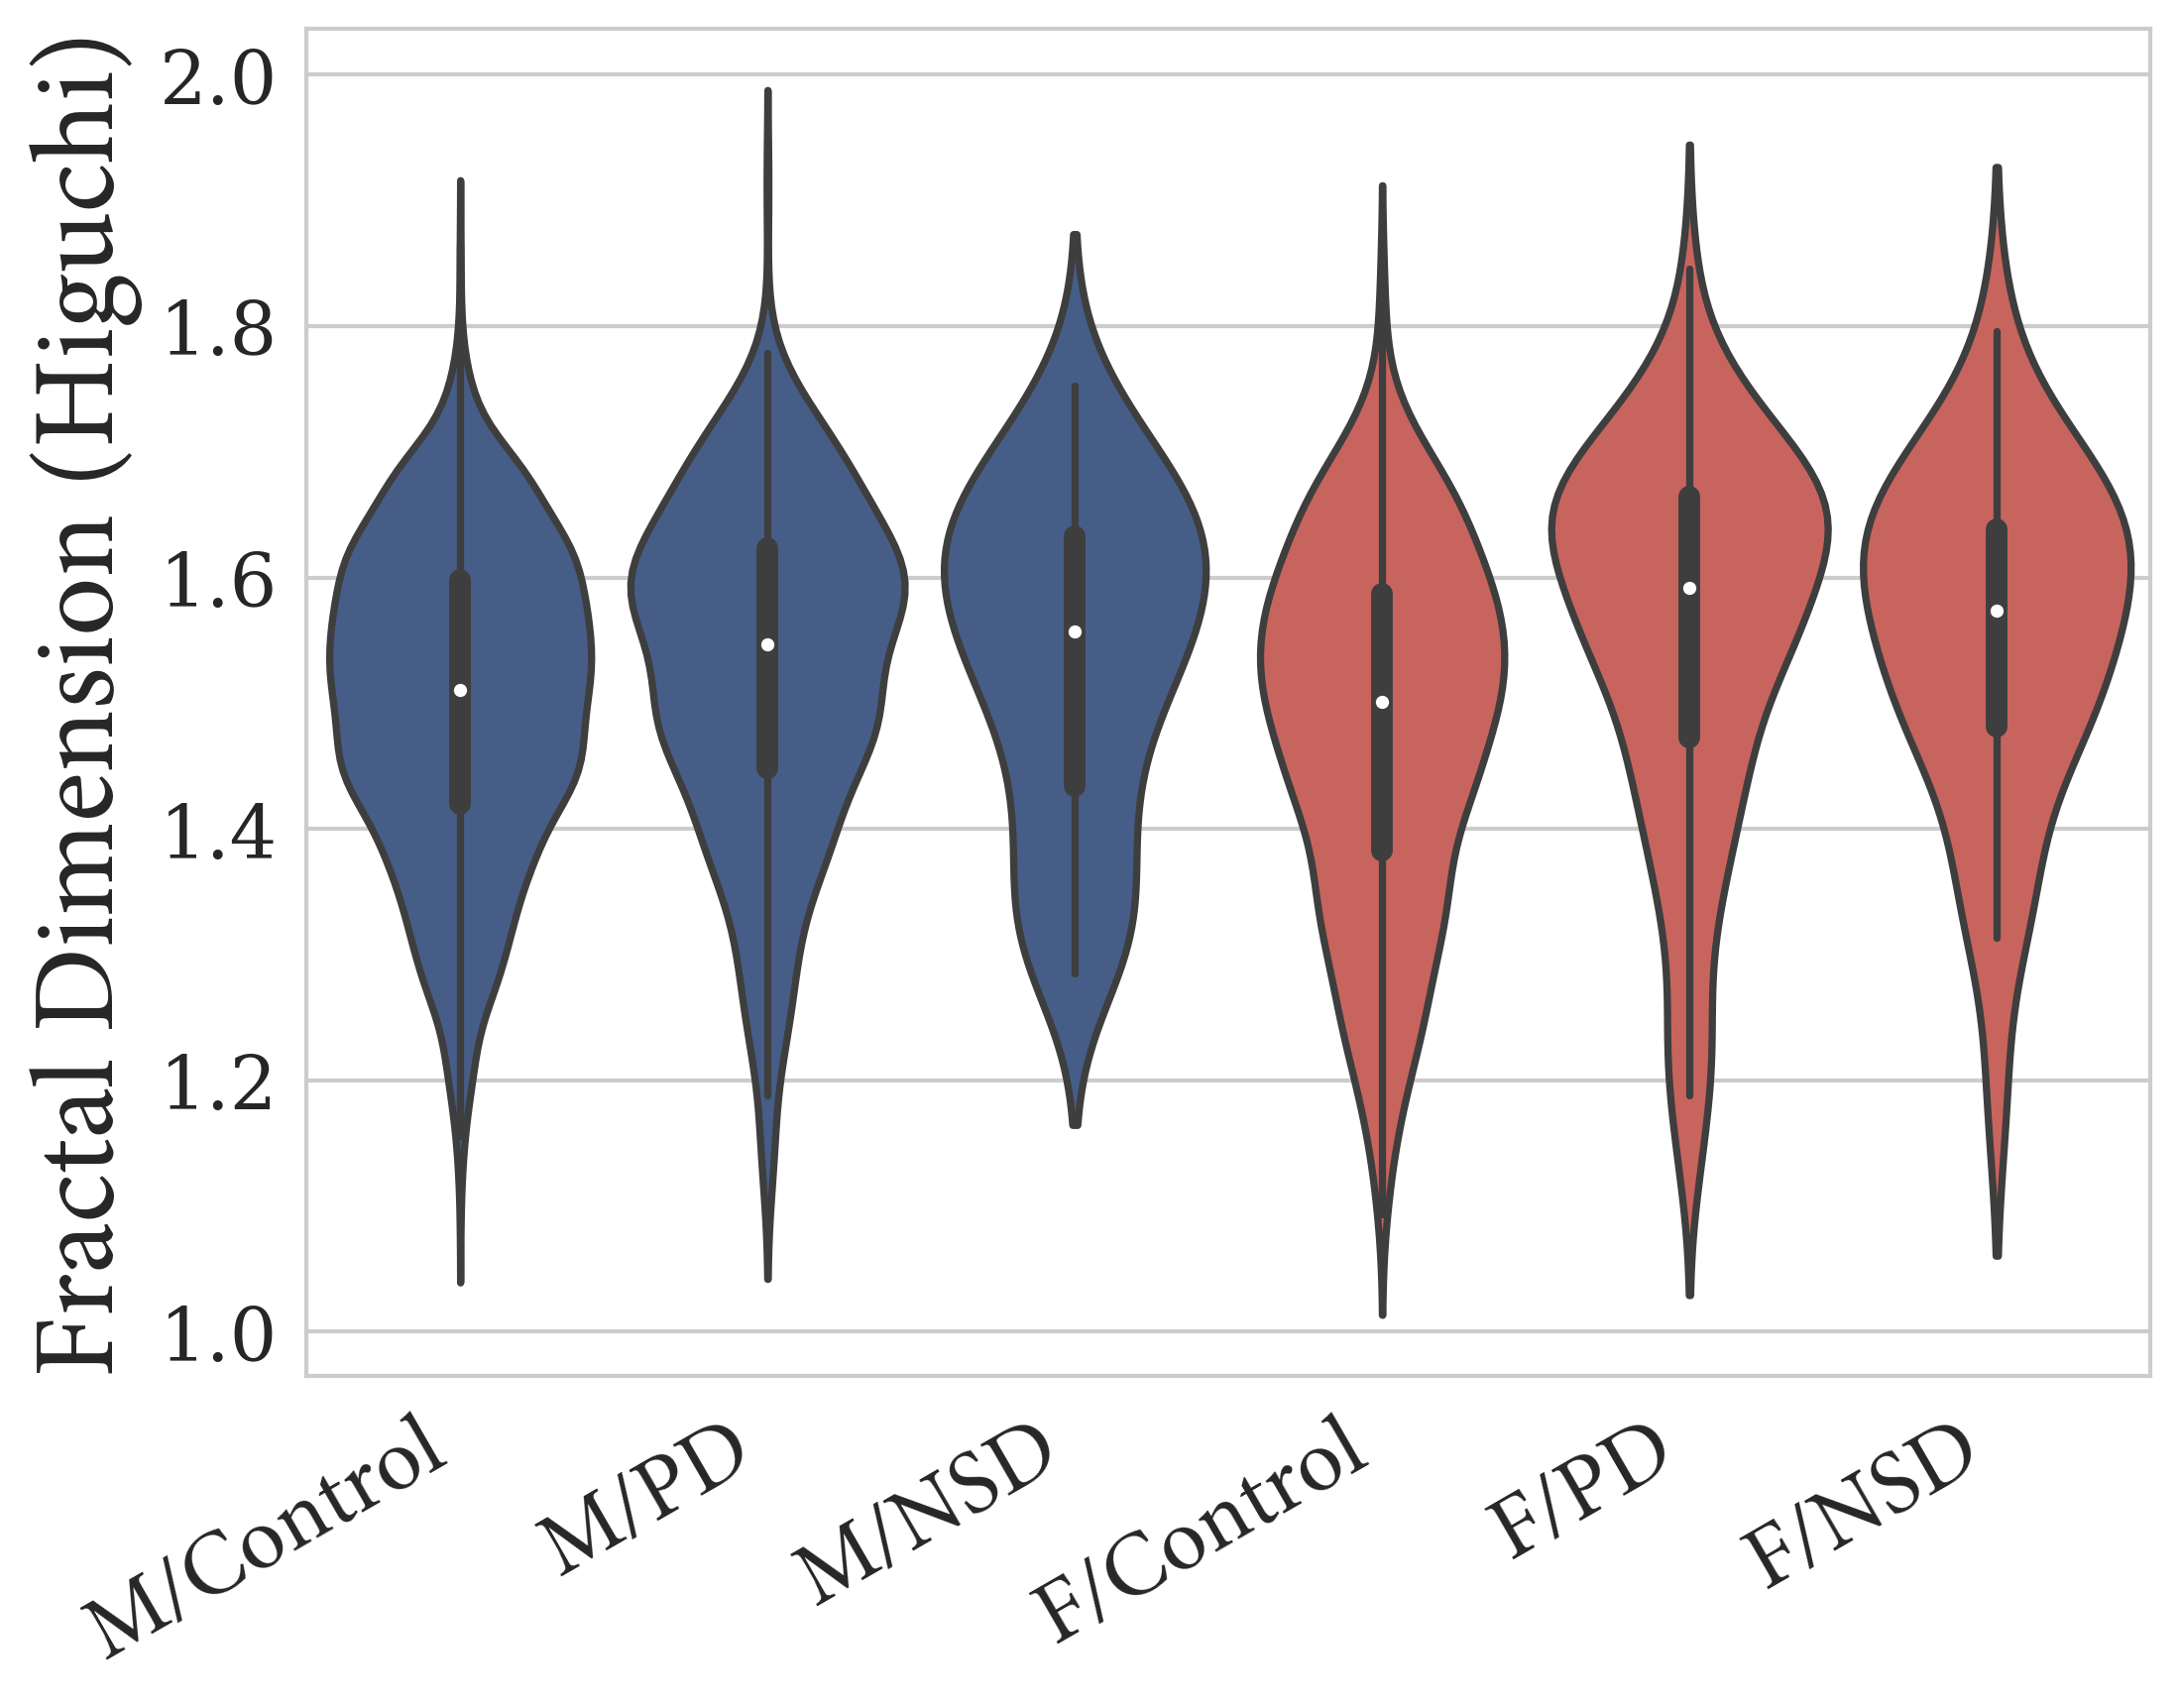
\includegraphics[width=0.96\linewidth]{HFD_boxplot.png}
		\end{subfigure}%
		\begin{subfigure}[]{0.52\textwidth}
			\label{sampenboxplot}
			\caption{Sample Entropy ($>0.15$ removed)}
			\centering
			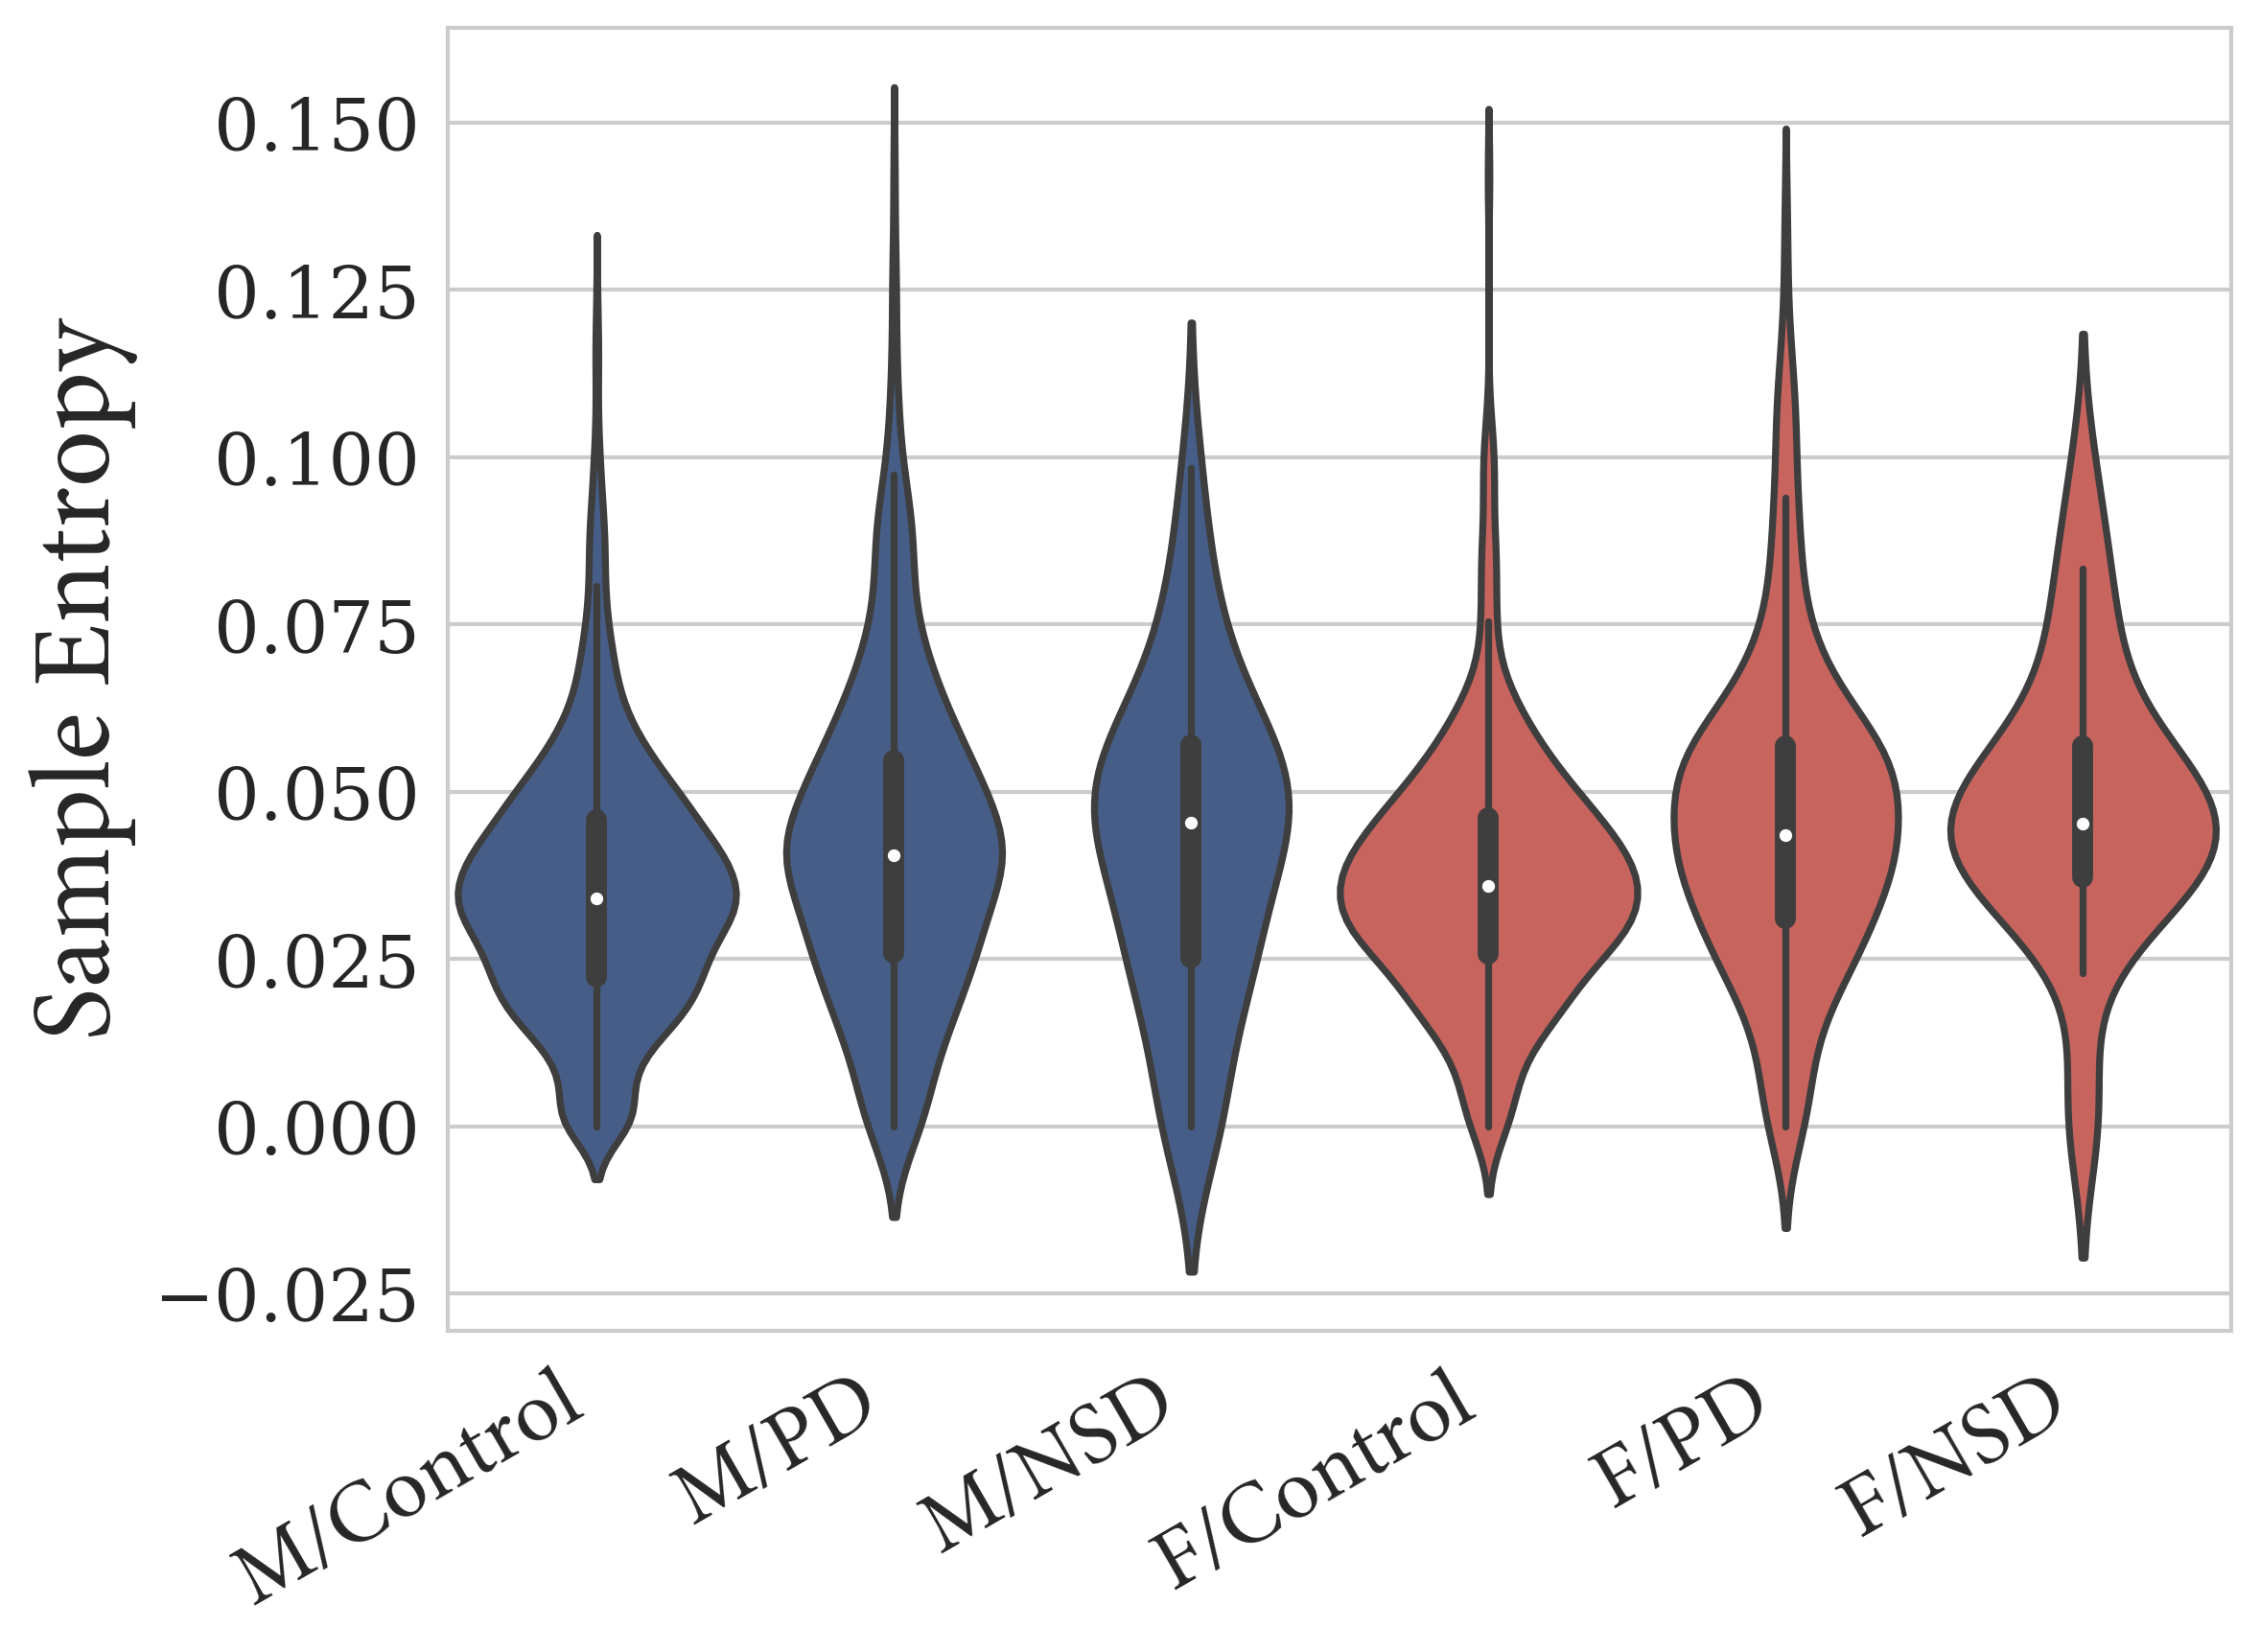
\includegraphics[width=0.96\linewidth]{sample_entropy_boxplot.png}
		\end{subfigure}
	}
	\caption{(a) The fractal dimension is likely inaudible, as PD and NSD are distributed similarly\textsuperscript{†} whereas control and NSD are different\textsuperscript{*} (b) The sample entropy is also likely inaudible, as PD and NSD are distributed similarly\textsuperscript{†} and control and NSD differently in males\textsuperscript{*} and females\textsuperscript{***}.}
	\label{hfdsampenboxplot}
\end{figure}


The fractal dimension and sample entropy are two features introduced from EEG signal processing. These features measure the signal's complexity and uncertainty, and are less biologically motivated than DFA and RPDE. In particular, these features often relate to detailed high frequency information, to which the human auditory system is less sensitive to~\cite{auditoryrange}. We  expect that the non-linear features introduced in \textit{\hyperref[eegsigproc]{Section}} \ref{eegsigproc} are some of the better differentiators of NSD and control as they quantify similarly abstract qualities of a signal.


As shown in \textit{\hyperref[hfdsampenboxplot]{Figure}} \ref{hfdsampenboxplot}, fractal dimension and sample entropy of a signal are unlikely to be audible qualities of a signal. It is a combination of these features which enable machine learning to differentiate healthy individuals and those with PD but no audible speech difficulties.

\begin{highlight}
	The novel features introduced in \textit{\hyperref[eegsigproc]{Section}} \ref{eegsigproc} were effective at differentiating individuals with invisible PD symptoms.
\end{highlight}

\newpage
\subsection{Significance of Findings}

From \textit{\hyperref[visfeature]{Section}} \ref{visfeature}, it is clear that making sense of each individual feature is a challenging task. Machine learning models are required to interpret the uncertainty of the features for a robust diagnosis. Prior models in this thesis have been constructed solely based on the characteristics of either a speech or walking signal. Including demographics information will significantly improve results. This is not solely due to the differences in PD amongst different genders and races ~\cite{gender,gendersymptoms,ageracial} --- demographics information also provides valuable information about the expected speech and gait characteristics.

Younger subjects were filtered out to create an approximate 50/50 split of the data and simulate more realistic diagnosis scenarios. Using the rule $\text{age}\geq35$ on phonation task, a set of 1591 individuals, 803 with PD and 75 with PD and no speaking difficulties remain. The rule $\text{age}\geq34$ on the movement task results in a set of of 775 individuals, 389 with PD. Our FWLS model with all novel features and demographics features achieves $82.1\pm2.7$ per cent classification accuracy on the phonation task and $81.7\pm3.3$ per cent on the walking task. These models did not use data augmentation or neural network based feature engineering, which are likely to further improve accuracy.

Although the performance of these machine learning models are insufficient to substitute neurologist diagnosis, they provide an effectively zero cost tool for neurologists to validate their diagnosis. Previously, we have shown that these machine learning models can detect dysphonia better than most humans (\textit{\hyperref[powerml]{Section}} \ref{powerml}) and it is likely that this is true for irregular gait. A positive result may be an sign to perform further checks on the patient. The results are especially good, considering many samples present in the mPower data may not be of suitable quality for diagnosis by a trained neurologist.

\begin{highlight}
	Although the current performance is not sufficient to replace neurologists, machine learning can be a valuable aid in the diagnosis process.
\end{highlight}

Additional data and cleaner data will always improve a classifier's performance, and we are far from reaching the limits of machine learning. In all models tested, over half of the mPower data was removed to allow for the 50PD:50C stratification. This left 1,700 subjects in the phonation task and 1,200 subjects in the walking task --- a sufficiently large sample for a good representation of the population; however, insufficient for such a complex task. This is evident in the significant improvements in results from simple data augmentation techniques in \textit{\hyperref[dataaugment]{Section}} \ref{dataaugment}. 


These diagnoses can be performed without the installation of any application on the user's phone. As a demonstration, we developed a web application which used the Javascript web audio and device motion APIs to record microphone and accelerometer data. The recordings were submitted to a basic (2GB RAM/single core) server which could perform diagnosis within 30 seconds running unoptimised code. The predictions are high variance --- taking the mean of multiple diagnosis on segments of each task (like data augmentation in \textit{\hyperref[dataaugment]{Section}} \ref{dataaugment}) greatly improved robustness at the cost of extra computation.

\begin{highlight}
It is extremely easy to place a trained machine learning model on the cloud --- making diagnosis or monitoring extremely cheap and easy.
\end{highlight}

It is clear machine learning can be a valuable tool for providing insights to neurologists. There is also enormous potential for growth --- as more data becomes available to machine learning models, their power and robustness will vastly improve. 


\newpage
\section{Implementation}
\label{implementation}
We would like to extend our thanks to all open-source libraries, and academics making their code publicly available. Without these, development would have been a significantly slower process. 

The project was primarily implemented in Python, acting as an interface between a number of libraries written in Matlab (Matlab Engine), R (rpy2) and C. The code for this project is published online at \url{https://github.com/maxwg/parkinsons-mpower}.

Wherever possible, reliable standard libraries or implementations used in previous research were preferred to maximise reproducibility and reliability. Standard speech features used in Interspeech were calculated using the official openSMILE~\cite{opensmile} program, which uses the sub-harmonic summation method of $f_0$ estimation~\cite{shs}. Most dysphonia-specific features were calculated using the toolbox published by Tsanas~\cite{spoverview} which uses the SWIPE~\cite{camacho2007swipe,f0estimation} $f_0$ estimation algorithm. 

Following Tsanas~\cite{spoverview}, 120hz and 190hz were used as the mean healthy $f_0$ for males and females respectively. Tsanas and Little~et~al.~\cite{splittlenonlinear2007} used an embedding dimension of 4 for non-linear features such as RPDE; however, our data suggested that 6 was more suitable. This was confirmed with features extracted in the embedding dimension of 6 being more informative in our classifiers. 

EEG and non-linear signal analysis was performed using the PyREM library~\cite{pyrem}, which builds upon PyEEG~\cite{pyeeg}, correcting some implementation flaws. The false nearest neighbour implementation in the pypsr~\cite{pypsr} library was used to calculate the embedding dimension for the relevant non-linear signal processing algorithms. The embedding dimension used in both speech and accelerometer was 6 and the embedding delay was chosen per sample as the first minimum of the approximate mutual information~\cite{rosenstein1993practicallyapunov}.
 
PyREM does not provide an implementation for Lyapunov Exponents and some experimentation with artificially constructed signals showed that PyEEG's implementation is severely wrong. The nolds~\cite{nolds} library was used to compute the Lyapunov exponents, using Rosenstein's~\cite{rosenstein1993practicallyapunov} algorithm for $\lambda^*$ and Eckmann's algorithm~\cite{eckmann1986liapunov} for $\lambda_1 - \lambda_6$.
  
Jerk based accelerometer features were considered~\cite{jerkfeature}; however, performance was generally worse than using the raw acceleration features over all computed measures. The DREAM challenge baseline features~\cite{mpowertools} were used in conjunction with our own implementation of the methods used in Arora~et~al~\cite{arora2014high}. The primary differences likely result from our preprocessing of the data, which rotated all accelerometers relative to the $x$ axis.


Traditional machine learning algorithms were mostly based on the standard scikit-learn~\cite{scikitlearn} implementation, with Gaussian processes implemented with GPy~\cite{gpy2014}. Hyperopt~\cite{hyperopt} was used to aid in finding the optimal hyperparameters for some models. Scikit-feature~\cite{skfeature} was used to implement the filter and embedded feature selection methods. Stacked regressions~\cite{stackregression} and Feature-weighted linear stacking~\cite{fwls} were implemented with the stacked\_generalization library~\cite{stackedgeneralizaton}.

Neural networks were primarily implemented in Keras~\cite{keras}. In general, ReLu~\cite{relu} was chosen as the activation and Nadam~\cite{nadam} used as the optimiser. Batch Normalisation~\cite{batchnorm} was applied whenever relevant and dropout~\cite{dropout} used to regularise the models. A sigmoidal node with a binary cross-entropy loss function used in binary classification. For regression of UPDRS scores, the Huber loss~\cite{huber1964robust} was selected.




\chapter{Conclusion}
Diagnosing Parkinson's disease with machine learning is a task far more difficult than what is suggested by prior literature. Replicating prior work on PD diagnosis with smartphones achieves just above 60 per cent performance --- a large decrease from the reported 98 per cent.  This reveals the dangers of machine learning in small datasets, with their results caused by either bias in the data and/or overfitting on cross validation.


We identify that results obtained in small datasets may not extrapolate outside of the dataset, and utilise the much larger mPower dataset. The mPower dataset consists of crowdsourced audio recordings of /aa/ phonation and a gait and balance task from 6,500 users, 1,100 with PD. We apply a number of novel features commonly used in EEG signal processing to the task, showing a noticable improvement. We then visualise and analyse some of these features, showing how noisy they are, and the necessity of machine learning to make sense of them.

Following a better understanding of the features, we then investigate the applicability of a number of strategies for improving machine learning performance: data augmentation, features selection and model ensembling. Data augmentation and model ensembling are shown to be highly effective, whereas feature selection selection is not.%, likely due to the machine learning models being used relatively robust to correlated features.

We then investigate the concept of automatic feature engineering with neural networks on the accelerometer data. Automatic feature engineering has been successfully applied on image and speech data, but applications to accelerometer data have been more limited~\cite{deepconvlstm}. We develop an architecture inspired by recent developments in speech recogntition~\cite{wavenet} and show that it is an extremely effective tool on top of traditional feature engineering. We did not have the resources to perform our stringent model evaluation strategy, so we took advantage of an unseen mPower test set released as part of the DREAM PD biomarker challenge. 

%XXXXXXXXXXXTODOTHE RESULTS.......

After developing the infrastructure for a reliable model to diagnose Parkinson's disease, we refer to our original question: ``is it possible for machine learning to detect symptoms imperceptible by humans?'' We had a hold-out set of 86 participants who marked themselves as having zero speech difficulty, verified by the researcher. We discovered that machine learning could diagnose these individuals as accurately as the other participants with more noticeable speech disabilities. The features enabling machine learning to achieve this were examined --- in particular, most novel measures introduced were strong differentiators of PD and inaudible. This is a very promising result for machine learning, and we finish with some recommendations on how to progress and ideas that we developed but did not explore.

\section{Where to? Recommendations for Future Research}

This thesis may be very information dense, yet covers only the beginning for what must be completed before machine learning can be applied in a medical context. Trust of machine learning is the biggest barrier. This can be developed by \emph{understanding} the behaviour of these machine learning models better, and recognising their strengths and weaknesses.

We have introduced many of features to diagnose Parkinson's disease from voice and gait, and only perform a preliminary analysis of a subset of these features. A thorough analysis on a cleaner dataset is desirable --- it may be the case that some features are good enough indicators of PD once the recording setup is controlled, and may be interpretable without machine learning. We have also noted that a number of features are not length-invariant --- developing length invariant alternatives or using a time stepped augmentation approach would greatly improve robustness.

As we have shown in \textit{\hyperref[automaticfeatureengineering]{Section}} \ref{automaticfeatureengineering}, neural networks are a powerful tool in the feature engineering process. However, there remains a lot to be desired in terms of understanding and interpretation of these networks. The behaviour of CNNs and LSTMs have individually been visualised~\cite{cnnvis, visualisernn} and there is still a significant amount of work to be done in understanding either architecture. Fusion Architectures combining both LSTM and convolution layers are even less understood~\cite{LRCN}, but they perform exceedingly well on time series data~\cite{convlstm}. 


Although machine learning may not be at a stage where it can be directly applied in a medical context, its ability to detect symptoms of Parkinsonian speech indistinguishable to humans is a very promising result for the field. This thesis only delves into a basic exploration of the features which allow machine learning to do this, and a more comprehensive analysis with more reliable data is required. It may be possible to visualise some inaudible features in the form of an oscilloscope or spectrogram.

Telemonitoring is one of the most promising applications of machine learning as small errors in predictions are tolerable. Setting up a smartphone telemonitoring platform would also provide a good source of data to train future machine learning models. Although telemonitoring has not been discussed in this thesis, the methods used in feature engineering are interchangeable. The biggest change would be the machine learning model, with Gaussian processes and neural networks more suitable for regression tasks. The work in this thesis has also been adapted and submitted to the second challenge of the DREAM PD biomarker competition~\cite{dreamchallengeinfo}, which involves predicting UPDRS scores from smartwatch accelerometer data.


There were many ideas developed in completing this project, and only a small subset could be explored. The diagnosis of Parkinson's disease commonly involves observing a subject's response to medication such as Levodopa~\cite{tolosadiagnosis26}. The mPower dataset has fields describing the medication state of participants with PD. Utilising this additional information and developing features measuring the differences before and after medication could significantly improve diagnosis accuracy.

Parkinson's disease motor symptoms are often presented asymmetrically, with studies showing 86 per cent of patients exhibit different symptoms on different sides of their body~\cite{pdasymmetry}. The biological mechanisms are not well understood~\cite{djaldetti2006mystery}; however, asymmetry in symptoms may be able to help differentiate Parkinson's disease from other similar disorders. With smartphone based data, measuring asymmetry would require repeated tests while holding the smartphone with either hand --- or like the second PD DREAM subchallenge, having smartwatches on both wrists. 

We explored some feature engineering work in the Interspeech challenges, which covers tasks ranging from emotion recognition to speaker trait recognition~\cite{is2009}. The features and approaches to these challenges are undoubtedly relevant to PD diagnosis via speech. In our limited exploration of the Geneva~\cite{geneva} and ComParE~\cite{compareis13featureset} feature sets, significant improvements were observed; however, these feature sets were not analysed in depth due to prioritising dysphonia specific and our novel features.

%active learning...? differntiation of PD and parkinsonian.

There is much more work to be done, and it is important that it is done in an open manner. Progress should be measured on standardised datasets, allowing for empirical comparisons between techniques. The actual numbers should not matter --- only that a performance increase has been observed. One of the biggest advantages of machine learning is that many basic methods can be ensembled into a high performing model with minimal effort~\cite{netflixprizebellkor}. Releasing code publicly so results can be easily replicated or extended will also be important in accelerating the field. Methods are becoming more complex and it can be very difficult to concisely summarise them in research paper format.



\section{A Finishing Note}
We advocate that measures such as accuracy and AUROC should be used for the purposes of model selection and not interpreted as the ability of a model to generalise to the real-world or to different datasets. Machine learning for Parkinson's disease is still in its initial stages, and controlling for dataset quality and ensuring a representative sample of the population at this stage would slow progress.

The importance of significance testing and careful cross validation to prevent overfitting should also be evident (\textit{\hyperref[detectoverfit]{Section}} \ref{detectoverfit}). As machine learning models continually improve, the benefits from improvements will become less significant. As improvements become more marginal, testing that an increase in performance is due to the improvement rather than natural variance in the machine learning model's predictive power will become necessary. 

The reader may have noticed that we discarded more than half of the mPower dataset to obtain a 50PD/50C stratification in the models we have trained. We have also demonstrated the power of automatic feature engineering, though have not applied it to our results. The goal of this thesis is not to present the best possible results, but rather to demonstrate the applicability of each individual approach. Machine learning enables us to ensemble the results of many individual improvements to develop more powerful models. Every little improvement matters, as evident in the Netflix prize, where all top teams involved large ensembles of smaller, simpler models~\cite{netflixprizebellkor}.



\backmatter

\bibliographystyle{ieeetr}
\bibliography{bib} % -> lee miarchivo.bib



\end{document}